\documentclass[12pt,openright,twoside,a4paper,english,french,spanish]{abntex2}
\input{fixos/pacotes}
\input{fixos/comandos}
\input{fixos/novoscomandos}

% Dados pessoais
\autor{Lucas de Lima Spinosa dos Santos \\ Rodrigo Carvalho dos Santos}
\curso{Engenharia de Software}

% Dados do trabalho
\titulo{Plataforma Web de Tutoria}
\data{2026}
\palavraChaveUm{Tutoria}
\palavraChaveDois{Sistema de Recomendação}

% Dados da orientacao
\orientador{Prof. Dr. Vandor Roberto Vilardi Rissoli}
% \coorientador{(quando houver, Titulação Acadêmica e Nome do Orientador)}

% Dados para a ficha catalográfica
\cdu{02:141:005.6}

% Dados da aprovação do trabalho
% \dataDaAprovacao{29 de agosto de 2025}
\membroConvidadoUm{Profa. Dra. Elaine Venson}
\membroConvidadoDois{Prof. Dr. Ricardo Ramos Fragelli}

\local{Brasília, DF}
\instituicao{%
  Universidade de Brasília - UnB
  \par
  Faculdade de Ciências e Tecnologias em Engenharia - FCTE
}
\tipotrabalho{Trabalho de Conclusão de Curso}
\preambulo{Monografia submetida ao curso de graduação em Engenharia de Software da Universidade de Brasília, como requisito parcial para obtenção do título 
de Bacharel em \imprimircurso.}

\input{fixos/setup}

\usepackage{float}
\usepackage{lscape}
\usepackage{tabularx}

\begin{document}

\frenchspacing 
\imprimircapa
\imprimirfolhaderosto*

\input{fixos/fichacatalografica}
% \input{editaveis/errata}
\input{fixos/folhadeaprovacao}
% \input{editaveis/dedicatoria}
% \input{editaveis/agradecimentos}
% \input{editaveis/epigrafe}

% ---------- DESCOMENTE O QUE FOR NESCESSÀRIO
\begin{resumo}

A educação é um pilar fundamental para o desenvolvimento de um país, mas o cenário educacional brasileiro enfrenta desafios como a baixa motivação e o desengajamento dos alunos, refletidos em indicadores como o Ideb e o PISA. Metodologias de aprendizagem colaborativa, como a tutoria, e a aplicação de gamificação têm demonstrado grande potencial para mitigar esses problemas, aumentando o engajamento e a eficiência do processo de ensino-aprendizagem. O objetivo deste trabalho é a implementação de uma aplicação web que intermedia o contato entre tutores de uma área de conhecimento e pessoas interessadas nesta tutoria. Trata-se de uma pesquisa aplicada, que utiliza procedimentos de pesquisa bibliográfica e metodologias ágeis de desenvolvimento de software. Ao final deste trabalho, foi implementada uma simulação da arquitetura para verificar a viabilidade da proposta, que se mostrou satisfatória ao atender os objetivos e validar a integração entre as tecnologias escolhidas para o êxito do projeto proposto.

 \vspace{\onelineskip}
    
 \noindent
 \textbf{Palavras-chaves}: Tutoria; Sistema de Recomendação; Gamificação; Aplicação Web.
\end{resumo}

\begin{resumo}[Abstract]
 \begin{otherlanguage*}{english}
    Education is a fundamental pillar for a country's development, but the Brazilian educational landscape faces challenges such as low motivation and student disengagement, reflected in indicators like Ideb and PISA. Collaborative learning methodologies, such as tutoring, and the application of gamification have shown great potential to mitigate these problems, increasing engagement and the effectiveness of the teaching-learning process. 
    The objective of this study was to develop a web application that mediates contact between tutors in specific fields of knowledge and individuals seeking tutoring. The platform provides features to search for and contact tutors, request sessions, and evaluate both tutors and learners after each interaction, utilizing gamification elements to foster engagement and consistent use of the application. It is an applied research, which uses bibliographic research procedures and agile software development methodologies. In the end of this work, a web application was developed and is currently available for use through standard web browsers.
   \vspace{\onelineskip}
 
   \noindent 
   \textbf{Key-words}: Tutoring; Recommendation System; Gamification; Web Application.
 \end{otherlanguage*}
\end{resumo}

\input{fixos/listasautomaticas}
\begin{siglas}
  \item[API] \textit{Application Programming Interface}
  \item[BTG] Beat the GMAT
  \item[CA] Critério de Aceitação
  \item[CASE] \textit{Computer-Aided Software Engineering}
  \item[CSS] \textit{Cascading Style Sheets}
  \item[DE-R] Diagrama Entidade-Relacionamento
  \item[DLD] Diagrama Lógico de Dados
  \item[DRF] \textit{Django Rest Framework}
  \item[E2E] \textit{end-to-end}
  \item[F] Funcionalidade
  \item[HTTP] \textit{Hypertext Transfer Protocol}
  \item[HTTPS] \textit{Hypertext Transfer Protocol Secure}
  \item[Ideb] Índice de Desenvolvimento da Educação Básica
  \item[JSON] \textit{JavaScript Object Notation}
  \item[JWT] \textit{JSON Web Tokens}
  \item[MBA] \textit{Masters in Business Administration}
  \item[MKO] \textit{More Knowledgeable Other}
  \item[MVC] \textit{Model-View-Controller}
  \item[MVP] Produto Mínimo Viável
  \item[MVS] \textit{Model-View-Serializer}
  \item[ORM] \textit{Object-Relational Mapping}
  \item[PISA] \textit{Programme for International Student Assesment}
  \item[QS-WUR] \textit{QS-World University Ranking}
  \item[RNF] Requisito Não Funcional
  \item[Saeb] Sistema de Avaliação Básica
  \item[SGBD] Sistema Gerenciador de Banco de Dados
  \item[SR] Sistema(s) de Recomendação
  \item[SRBC] Sistema(s) de Recomendação Baseada em Conteúdo
  \item[SRC] Sistema de Recomendação Colaborativa
  \item[SRH] Sistema(s) de Recomendação Híbridos (SRH) 
  \item[TCC] Trabalho de Conclusão de Curso
  \item[TDD] \textit{Test Driven Development}
  \item[UI] \textit{User Interface}
  \item[UnB] Universidade de Brasília
  \item[US] \textit{User Story}
  \item[USP] Universidade de São Paulo
  \item[XP] \textit{eXtreme Programming}
  \item[ZDP] Zona de Desenvolvimento Proximal
\end{siglas}
% \input{editaveis/simbolos} % Não utilizamos nenhum simbolo até o momento
\input{fixos/indiceautomatico}

\textual

\chapter[Introdução]{Introdução}
\label{cap:introducao}

\section[Contextualização]{Contextualização}
\label{sec:contextualizacao}

Um importante aspecto para o desenvolvimento de um país é a educação. Através dela, muda-se a vida tanto de pessoas em sua individualidade quanto no coletivo. Qualificação de mão de obra, novas descobertas tecnológicas, entre outros pontos positivos tornam importante o investimento e desenvolvimento de uma boa educação para os cidadãos de uma nação, e o Brasil não é exceção.

O Índice de Desenvolvimento da Educação Básica (Ideb) é um indicador da qualidade da educação brasileira criado em 2007, visando apurar a qualidade dos ensinos fundamental (separado em anos iniciais do 1° ao 5° ano e em anos finais do 6° ao 9° ano) e médio. Seu resultado leva em conta duas medições: os dados sobre aprovação escolar, obtidos no Censo Escolar, e as médias de desempenho no Sistema de Avaliação Básica (Saeb). O índice varia de 0 a 10, sendo que um valor 6 é equivalente ao sistema educacional de um país desenvolvido \cite{inep2024indicador}.

Entretanto, nota-se que chegar a tal valor ainda é um desafio. Em 2023 o Brasil alcançou nota 6 nos anos iniciais ensino fundamental (1° ao 5° ano), 5 nos anos finais fundamental (6° ao 9° ano) e 4,3 no ensino médio, aumentando apenas 0,1 porcento se comparado a anos anteriores. Em todos os casos, o ensino público sempre obtém pior desempenho \cite{ferreira2024educacao}. 

Existem diferentes metodologias de aprendizagem, sendo algumas delas de aprendizagem colaborativa, onde estudantes se ajudam em seu processo de aprendizagem. Uma delas é a monitoria estudantil, em que um aluno já aprovado em uma disciplina auxilia outros estudantes na aprendizagem dela. Nos cursos superiores, a monitoria tem sido utilizada com muita frequência como estratégia de apoio ao ensino, especialmente para atender estudantes com dificuldades de aprendizagem. Ao atuar como monitor(a), o estudante auxilia o(a) professor(a) no processo de ensino-aprendizagem, aprofunda seus conhecimentos na determinada disciplina e propicia ao graduando desenvolver o interesse pela carreira docente, pois convive com a prática diária do ensino \cite{gonccalves2021importancia}.

Uma metodologia similar é a Trezentos, criada por Ricardo Fragelli. Uma avaliação individual é aplicada na turma de uma disciplina e, após os resultados, estudantes são agrupados em grupos de cinco a seis membros, de maneira que os com alto rendimento se unem aos com baixo rendimento, e os auxiliam na realização de metas estabelecidas pelo professor para que os estudantes com baixa nota do grupo tenham a chance de refazer a avaliação \cite{trezentos}. Em 2015, o índice de aprovação na disciplina Cálculo 1 da Universidade de Brasília (UnB) no campus Gama com a aplicação do Trezentos  subiu de 50\% para 95\% \cite{trezentosResultados}. Essas duas metodologias provam que, de fato, a aprendizagem colaborativa pode ser muito eficaz.

Percebe-se que, de forma geral, há uma crise motivacional, principalmente no que tange ao cenário educacional. Grande parte das instituições de ensino, independente de nacionalidade e de níveis de educação, encontra dificuldades para engajar seus alunos utilizando os recursos educacionais tradicionais. Uma metodologia recente que ajuda a mitigar o problema é a gamificação, que consiste na utilização de elementos de jogos fora do contexto deles, para promover a aprendizagem, motivando os aprendizes a alguma ação e auxiliando na solução de problemas e na interação com outros estudantes  \cite{tolomei2017gamificaccao}.

Elementos da gamificação incluem sistemas de pontuação, níveis, ranking, medalhas, desafios, entre outros recursos mais comuns aos jogos. Trabalhando com pontuações e níveis de experiência, o usuário é instigado a buscar atividades a fim de cumprir metas e atingir objetivos. Esses fatores dialogam entre si, aumentando o senso de socialização e colaboração, sem contar o aumento de \textit{feedback} contínuo, proporcionando a noção do progresso em uma atividade realizada durante o processo de aprendizagem \cite{tolomei2017gamificaccao}.

Diante dos fatores citados, um software que forneça a oportunidade de intermediar o contato entre pessoas que dominam uma área do saber e estudantes interessados em aprender e que utilize elementos de gamificação para manter o engajamento de ambas as partes tem potencial de auxiliar na aprendizagem de estudantes com dificuldade de aprendizagem.


\section[Questão de Pesquisa]{Questão de Pesquisa}
\label{sec:questao}

Com o objetivo de nortear o desenvolvimento do trabalho, a seguinte questão de
pesquisa foi definida:

\textit{Como uma plataforma pode auxiliar estudantes com dificuldades em uma área de conhecimento e pessoas versadas nesta área a se conectarem e agendarem encontros ao mesmo tempo que os mantém engajados a usá-la por tempo prolongado, aumentando a assimilação e fixação de conhecimento?}

\section[Justificativa]{Justificativa}
\label{sec:justificativa}
% Por que? Para melhorar a capacidade de aprendizagem

A situação da educação é um problema de longa data no Brasil. Além dos resultados nacionais do Ideb mencionados anteriormente, o desempenho do país se encontra entre as piores posições em avaliações internacionais, como por exemplo o \textit{Programme for International Student Assesment} (PISA) na educação básica e \textit{QS-World University Ranking} (QS-WUR) na educação superior.

O Brasil obteve as seguintes posições no ano de 2022: entre 62ª e 69ª posição no PISA em matemática, entre 44ª e 57ª posição em leitura e entre 53ª e 64ª posição em ciências \cite{pisa2024}.
Enquanto na lista de 92ª posição  no QS-WUR, em que apenas a Universidade de São Paulo (USP) aparece entre as universidades do pais no top 100 do ranking, as demais universidades do Brasil ficam em posições maiores de 200 \cite{qswur2025}.

Não é incomum que cada vez mais alunos se encontrem desinteressados e dispersos pelo conteúdo em sala de aula, principalmente com as metodologias de aprendizagem, as quais são majoritariamente passivas \cite{fragelli2017game}.

Um fenômeno emergente é a gamificação, que deriva da popularidade dos \textit{games}, e da capacidade intrínseca de motivar ação, resolver problema e melhorar aprendizagem nas diversas áreas do conhecimento humano \cite{fardo2013gamificacao}.
No campo educacional, a gamificação tem sido utilizada cada vez mais, superando
os métodos tradicionais de ensino e aprendizagem pelos games \cite{souza2025metodologias}.

A gamificação é a infusão intencional de elementos e mecânicas de jogos em situações que não são de jogos. O objetivo principal é engajar os participantes ativamente, motivá-los e ajudá-los a alcançar objetivos específicos. Essa abordagem aproveita nossas tendências naturais, como o desejo de competição, o senso de realização, o trabalho em equipe e o altruísmo, para impulsionar a participação, o desempenho e a satisfação geral \cite{magtani2024design}.

Há vários artigos com relatos de experiências de professores ao redor do mundo que utilizaram esses métodos em diversas áreas do conhecimento, da educação infantil ao ensino superior, obtendo resultados positivos \cite{fragelli2017game}.

Beat the GMAT (BTG) é a maior rede social do mundo para os candidatos de MBA (\textit{Masters in Business Administration}), atendendo a mais de 2 milhões de pessoas a cada ano. A BTG habilita as pessoas a aprender, compartilhar, ensinar e apoiar uns aos outros ao longo do processo de admissão de MBAs de grandes universidades. Essa empresa adotou a gamificação para aumentar o engajamento e retenção de seus usuários \cite{tolomei2017gamificaccao}.

A BTG foi configurada para, com base em determinados comportamentos, o usuário ser recompensado e ter em seu perfil essas recompensas. Um exemplo é a medalha ``Campeão da Gramática'' para usuários que escrevem 100 postagens no fórum de correção de gramática \cite{tolomei2017gamificaccao}.

Com essas e outras ações gamificadas, a BTG aumentou o tempo gasto por seus usuários em seu site e em sua comunidade em 370\%, significando um engajamento maior dos usuários nas atividades propostas. Além disso, a proposta gamificada trouxe aumento de 195\% de visitação em suas páginas, proporcionando à empresa uma possibilidade maior de conversão em novos usuários \cite{tolomei2017gamificaccao}.

Diante desses fatos, o tema deste trabalho se mostrou muito interessante, pois propõe unir duas abordagens educacionais em uma única plataforma, sendo potencialmente útil para a aprendizagem de alunos com problemas educacionais.

% O que? Plataforma de tutoria online

% Desta forma, este trabalho visa propor o desenvolvimento de uma plataforma de tutoria online, com elementos de gamificação, com o intuito mitigar o problema com a educação do Brasil. Incentivando tutores e alunos a se manterem engajados em ensinar e aprender.

% Quem? Tutores e alunos
% Qual?
% Aspectos positivos
% Aspectos impactos

\section[Objetivos]{Objetivos}
\label{sec:objetivos}

\subsection[Objetivo geral]{Objetivo Geral}

Este trabalho tem como objetivo geral propor a implementação de uma aplicação web que intermedia o contato entre tutores de uma área de conhecimento e pessoas interessadas nesta tutoria.

\subsection[Objetivos específicos]{Objetivos Específicos}

\begin{itemize}
    \item Estruturar um ambiente virtual que otimize a busca e conexão entre aprendizes e tutores, utilizando filtros parametrizados para facilitar a localização de tutores na área de conhecimento desejada;
    
    \item Aplicar técnicas de sistemas de recomendação para personalizar a sugestão de tutores, visando mitigar a sobrecarga de escolha e aumentar a relevância dos resultados para o aprendiz;
    
    \item Utilizar estratégias de gamificação para estimular a motivação e sustentar o engajamento de longo prazo de tutores e aprendizes na plataforma;

    \item Sistematizar o processo de agendamento de sessões de tutorias para assegurar a conciliação de horários e a organização das sessões;
    
    \item Viabilizar mecanismos de interação e \textit{feedback} direto entre os tutores e os aprendizes para consolidar a confiança e a construção de reputação dentro da comunidade da aplicação.
    
\end{itemize}

\section[Metodologias]{Metodologias}
\label{sec:metodologia}

As metodologias deste trabalho podem ser divididas em metodologia de pesquisa e metodologia de desenvolvimento.

Uma metodologia de pesquisa é caracterizada por sua abordagem, natureza, objetivo e procedimentos \cite{gerhardt2009metodos}. A metodologia de pesquisa deste trabalho tem abordagem qualitativa, natureza de pesquisa aplicada, objetivo de pesquisa exploratória e pesquisa bibliográfica como procedimento.

A metodologia de desenvolvimento de software utilizada consiste em uma adaptação da metodologia \textit{eXtreme Programming} (XP), com adição da forma de acompanhamento do \textit{Kanban}, levando em consideração o escopo do projeto, e também considerando apenas os dois alunos como desenvolvedores. Essas metodologias serão melhores explicadas no Capítulo \ref{cap:metodologia}.

\section[Organização do Trabalho]{Organização do Trabalho}
\label{sec:organizacao}
Este trabalho foi dividido em cinco capítulos, sendo esses resumidos da seguinte maneira:

\begin{itemize}
    \item Capítulo \ref{cap:introducao}: este capítulo introduz o tema do trabalho, compreendendo assim à \nameref{sec:contextualizacao}, \nameref{sec:questao}, \nameref{sec:justificativa}, \nameref{sec:objetivos} e \nameref{sec:metodologia}.

    \item Capítulo \ref{cap:referencial}: este capítulo sintetiza os principais conhecimentos teóricos que fornecem a melhor compreensão do contexto no qual o trabalho está envolvido, sendo este dividido em quatro seções: \nameref{sec:tutoria}, \hyperref[sec:aw]{Aplicação Web}, \hyperref[sec:recomendação]{Sistemas de Recomendação} e \hyperref[sec:gamificacao]{Gamificação}.

    \item Capítulo \ref{cap:metodologia}: este capítulo apresenta a proposta do trabalho, esclarecendo os principais aspectos quanto à metodologia utilizada, tecnologias escolhidas, requisitos definidos, arquitetura de software e desenvolvimento do trabalho proposto.
    
    \item Capítulo 4: este capítulo apresenta a execução da proposta, bem como as mudanças necessárias para o sucesso da implementação.

    \item Capítulo 5: este capítulo finaliza o projeto proposto, apresentando os resultados alcançados e trabalhos futuros relacionados ao projeto.
\end{itemize}
\chapter[Referencial Teórico]{Referencial Teórico}
\label{cap:referencial}

Neste capítulo serão abordados os principais conceitos e assuntos associados aos estudos e as realizações importantes à melhor compreensão de seu contexto e o desenvolvimento condizente as demandas identificadas.

\section[Tutoria]{Tutoria}
\label{sec:tutoria}

A prática de uma pessoa mais experiente ensinar ou orientar uma pessoa mais novata no estudo ou no exercício de uma determinada atividade pode receber diversos nomes a depender do contexto: mentoria, tutoria ou monitoria.

Sendo assim, é importante explicar cada um dos conceitos citados para melhor discernimento do que o projeto visa alcançar, contribuindo ainda com o melhor esclarecimento sobre cada um deles e suas diferenças.

Mentor é um indivíduo experiente que tem por objetivo passar adiante suas experiências e vivências em uma determinada área de atuação. Normalmente age como uma referência, uma pessoa disposta a demonstrar tudo o que sabe, orientando, apontando direções e estabelecendo desafios que permitam ao aprendiz que está sendo orientado, denominado mentorado, desenvolver seu conhecimento a partir de suas experiências \cite{oliveira2020mentoria}.

A mentoria é um acompanhamento de longo prazo e marcada por uma relação de respeito e confiança entre o mentor e o mentorado, envolvendo aspectos de carreira e apoio psicológico \cite{oliveira2020mentoria}. Entretanto, o mentor tem um papel que ultrapassa a orientação para estudo, buscando também o desenvolvimento pessoal e psicossocial do mentorado \cite{botti2008preceptor}. Exemplos incluem a aquisição de competências socioemocionais e cognitivas e a melhoria da autoestima e autorregulação \cite{opp2024mentoria}.

Essa natureza pessoal da mentoria é presente desde o poema que deu origem a essa palavra: \textit{Odisseia} de Homero, em que Odisseu confia a Mentor, seu fiel e sábio amigo, a educação de seu filho Telêmaco antes de partir para a guerra de Tróia. Atena, deusa da sabedoria e da razão, assume a forma de Mentor e orienta Telêmaco no seu desenvolvimento físico, intelectual e espiritual \cite{semiao2009tutoria}.

Tutoria pode ser definida como uma relação de ajuda entre duas pessoas com diferentes níveis de conhecimento, competências e/ou experiências em que o tutorando, o indivíduo de menor capacidade, recebe apoio do tutor para superar dificuldades escolares ou acadêmicas \cite{opp2024mentoria}. O tutor não necessariamente não precisa ser um docente formal, podendo ser um familiar, estudante ou um voluntário \cite{topping2000tutoring}.

A tutoria existe desde a Antiguidade, onde a cultura de povos e valores como honra, justiça e honestidade eram passados pelos tutores para seus aprendizes. A partir das universidades na Idade Média a tutoria passou também a ser acadêmica, com tutores sendo alunos mais velhos que ensinavam habilidades como leitura e interpretação de texto para os estudantes mais jovens, sob supervisão de um docente \cite{geib2007tutoria}.

Comparado com o aprendizado tradicional com um professor, a tutoria pode fornecer mais experiência prática, mais atividades e variedade e também mais ajuda individualizada \cite{topping2000tutoring}. Embora parecidas, a tutoria e a mentoria se diferem em seus objetivos, visto que a tutoria visa ajudar na superação de dificuldades através do ensino de conteúdos ou competências específicas, sem buscar ativamente o desenvolvimento pessoal \cite{opp2024mentoria}. Entretanto, este ainda pode vir a ocorrer como consequência das interações, como aumento da autoconfiança e desenvolvimento de pensamento crítico, tanto para o tutor quanto para o tutorando \cite{lin2025peer}.

Monitoria é uma atividade que surgiu na Idade Média, e consiste em um estudante mais experiente de uma turma auxiliar o professor no ensino de colegas de classe mais novatos. Na metade do século XIV, os professores tinham quase sempre um monitor que os auxiliavam na escolarização. No século XVIII existia o Método Monitorial de Lancaster na Inglaterra, em que adolescentes, instruídos diretamente pelos mestres, atuavam como monitores ensinando outros adolescentes \cite{frison2016monitoria}. Nota-se que a monitoria continua a ser usada até os dias atuais.

No Brasil, o programa de monitoria está regulamentado pelas instituições de ensino superior e tem como finalidade promover a participação de estudantes com desempenho destacado em disciplinas, atuando como facilitadores da aprendizagem dos colegas e colaborando com o docente na construção de metodologias de ensino \cite{monitoria2025}.

Assim como na tutoria, ambos monitor e estudante se beneficiam da monitoria. O estudante recebe apoio no aprendizado do conteúdo da disciplina e o monitor desenvolve competências acadêmicas, sociais e profissionais, como comunicação, liderança, empatia e didática, além de seu engajamento em programas de monitoria poder abrir portas para novas oportunidades acadêmcias, como a participação em projetos de pesquisa e extensão \cite{monitoria2025}.

Diante do exposto, o modelo de interação pretendido pelo projeto é a tutoria, focada no aprendizado de conteúdos e habilidades específicas, não sendo o objetivo o desenvolvimento pessoal em conjunto com o aprendizado, inerente à mentoria, e não possuindo o caráter acadêmico intrínseco à monitoria. Entretanto, a tutoria pode evoluir para uma mentoria caso se forme um vínculo entre o tutor e o tutorado e o tutor queira o ajudar com seus problemas pessoais, passando a ser um mentor para o mesmo.

Neste trabalho, a aprendizagem é compreendida sob a ótica da Teoria da Aprendizagem Significativa de David Ausubel, que define aprendizagem como a organização e
integração de informações na estrutura cognitiva do indivíduo. De acordo com a teoria, a aprendizagem é significativa quando os novos conceitos são compreendidos e relacionados com conhecimentos prévios do indivíduo, criando conexões significativas e sendo mais provável de ser transferida para a memória de longo prazo, enquanto que uma aprendizagem mecânica ocorre quando o indivíduo não realiza tais conexões, simplesmente memorizando fatos e informações sem entender os princípios ou conexões subjacentes, podendo ocorrer descarte como conhecimento sem relevância, sem significado e sem sentido \cite{junior2023olhar}.

Considerando que o fator isolado mais importante para a aprendizagem é o que o aprendiz já sabe, a tutoria se apresenta como um mecanismo ideal para esse processo, pois permite que o tutor identifique os conhecimentos prévios do aprendiz e facilite a absorção da nova informação, promovendo a retenção do conhecimento e evitando a aprendizagem mecânica.

Adicionalmente, a dinâmica da tutoria é compreendida neste trabalho como um processo de aprendizagem colaborativa, fundamentado na perspectiva sociointeracionista de Lev Vygotsky. Segundo \citeonline{saul2025}, essa abordagem concebe o desenvolvimento cognitivo e o aprendizado como inerentemente sociais, mediados pela interação entre indivíduos com diferentes níveis de conhecimento. Nesse cenário, o aprendizado ocorre quando um indivíduo realiza uma tarefa ou atividade que está além de suas capacidades recebendo o suporte de uma pessoa ou recurso com mais conhecimento do que ele, denominado More Knowledgeable Other (MKO, ou "Outro Mais Conhecedor"). Através do compartilhamento do conhecimento, dicas e encorajamento, o aprendiz acessa sua Zona de Desenvolvimento Proximal (ZDP), justamente o espaço entre o que consegue fazer sozinho e com ajuda, internalizando novas habilidades e podendo se tornar um MKO para outros aprendizes.  

Para viabilizar a busca e o contato com os tutores de forma acessível, a solução proposta é o desenvolvimento de uma aplicação web. Esta plataforma servirá como um ambiente digital onde os usuários poderão não apenas buscar por especialistas, mas também realizar o contato inicial e agendamento das sessões de aprendizado.

\section[Aplicação Web]{Aplicação Web}
\label{sec:aw}

% O projeto visa desenvolver uma aplicação web.
Uma aplicação web é um programa computacional que é executado através de um navegador de Internet, também chamado de \textit{browser}, como Google Chrome, Mozilla Firefox e outros, com o objetivo de executar funções, como um formulário de contato ou uma calculadora. Exemplos de aplicações web são Google Docs e Microsoft Office 365 \cite{harwood2022internet}.

Segundo \citeonline{shklar2009web}, uma aplicação web é diferente de um \textit{website}. Um \textit{website} é essencialmente informativo, projetado para fornecer conteúdo de forma estática, semelhante a um folheto digital ou a um site de notícias, não necessariamente oferecendo funcionalidades. Essa distinção é reforçada por \citeonline{delaRosa2025webapp}, que destaca diferenças adicionais, como o nível de interatividade. \textit{Websites} tendem a oferecer menor interatividade, geralmente limitando-se a ações básicas, como navegação por \textit{links}, enquanto aplicações web permitem interações mais complexas, como envio de arquivos, preenchimento de formulários e edição de documentos, por serem projetados para oferecer funcionalidades para o usuário. 

Aplicações web são programas elaborados sob uma arquitetura cliente/servidor \cite{shklar2009web}. Segundo \citeonline{nyabuto2024architectural}, essa arquitetura funciona baseada no envio de requisições e respostas, em que o cliente inicia a comunicação enviando um pedido (requisição) e o servidor processa esse pedido e retorna uma resposta ao cliente. Na aplicação proposta, um exemplo de comunicação é o aprendiz buscar tutores, enviando uma requisição para o servidor, que a processa e retorna uma lista de tutores (resposta) para o aprendiz.

A interação do usuário com uma aplicação web pode ser considerada um diálogo. O cliente (usuário) fornece dados ou clica em elementos da interface, como um botão, para realizar uma ação. A aplicação então fornece uma resposta para a ação do usuário, como exibir dados em resposta a submissão de um formulário de pesquisa, que pode então gerar uma nova ação do usuário \cite{harwood2022internet}.

Para enriquecer a experiência na aplicação, serão implementadas duas estratégias principais. Primeiramente, um sistema de recomendação será desenvolvido para garantir que os usuários encontrem tutores compatíveis com seus interesses e necessidades. Adicionalmente, para promover o uso contínuo e manter os usuários engajados, serão aplicados elementos de Gamificação.

\subsection[Sistema de Recomendação]{Sistema de Recomendação}
\label{sec:recomendação}

Os Sistemas de Recomendação (SR) são algoritmos feitos para sugerir itens relevantes para usuários, sejam estes itens produtos, serviços, informações, etc. Normalmente os SR estão em aplicações web, aprendendo com interações anteriores dos usuários e/ou com atributos dos itens \cite{Aggarwal2016}. Esses sistemas ajudam os usuários a encontrarem itens de interesse em grandes conjuntos de dados, priorizando ou filtrando alternativas com base no histórico do usuário, preferências ou comportamentos similares de outros usuários \cite{Francesco2015}.

O Sistema de Recomendação Colaborativa (SRC) visa adquirir informações sobre o comportamento prévio ou as opiniões de um grupo de usuários existente para premeditar quais itens o usuário atual do sistema provavelmente irá gostar ou se interessar. Atualmente, esses tipos de sistemas são amplamente utilizados na indústria, especialmente como uma ferramenta em \textit{sites} de varejo \textit{online} para personalizar o conteúdo de acordo com as necessidades de um determinado cliente. Estas abordagens colaborativas usam uma matriz de classificações de itens de usuários como única entrada e normalmente produzem os seguintes tipos de saída: uma previsão (numérica) indicando até que ponto o usuário atual gostará ou não gostará de um determinado item e uma lista de \textbf{\textit{n}} itens recomendados. Essa lista dos \textbf{\textit{n}} melhores itens não deve, obviamente, conter itens que o usuário atual já tenha adquirido \cite{Jannach2011}. 

Nos Sistemas de Recomendação Baseados em Conteúdo (SRBC) os atributos descritivos dos itens são usados para fazer recomendações. O termo ``conteúdo'' refere-se a essas descrições. Nos métodos baseados em conteúdo, as classificações e o comportamento de aquisição dos usuários são combinados com as informações de conteúdo disponíveis nos itens. Nos métodos baseados em conteúdo as descrições de itens, que são rotuladas com classificações, são usadas como dados de treinamento para criar uma classificação específica do usuário ou um problema de modelagem de regressão. Para cada usuário, os documentos de treinamento correspondem às descrições dos itens que ele comprou ou classificou. A variável de classe (ou dependente) corresponde às classificações especificadas ou ao comportamento de aquisição. Esses documentos de treinamento são usados para criar um modelo de classificação ou regressão, que é específico para o usuário em questão (ou usuário ativo). Esse modelo específico do usuário é usado para prever se o indivíduo correspondente gostará de um item cuja classificação ou comportamento de aquisição é desconhecido \cite{Aggarwal2016}.

Os Sistemas de Recomendação Híbridos (SRH) surgem como uma opção interessante ao combinar diversas técnicas ou algoritmos, visando unir os pontos positivos de diferentes métodos, a fim de atender suas fraquezas e melhorar a eficiência das recomendações. A Recomendação Colaborativa é baseada na avaliação das preferências dos usuários e no comportamento coletivo da comunidade, a fim de produzir sugestões com base nas semelhanças entre perfis de usuários. Em contrapartida, os Sistemas de Recomendação Baseados em Conteúdo se valem de atributos próprios dos itens, como suas características estruturais e descrições em texto, para determinar a relevância pessoal de interações. Embora ambas as metodologias tenham benefícios reconhecidos, cada uma tem suas limitações específicas — como a limitação de dados na filtragem colaborativa quando pouco ou nenhum perfil de usuário para comparação e a insuficiência de variedade nas recomendações que se baseiam apenas no conteúdo \cite{Jannach2011}.

% Com base no exposto, e visando a maior compatibilidade possível entre usuários e tutores na aplicação proposta, optou-se pela implementação de um SR Híbrido. A escolha se justifica por combinar as forças das abordagens de conteúdo e colaborativa, mitigando suas fraquezas individuais.

% Em suma o componente baseado em conteúdo (SRBC) será responsável por recomendar tutores com base em atributos explícitos, como a área de conhecimento ou habilidade que o usuário busca (por exemplo, "Aulas de Violão"). Em paralelo, o componente de filtragem colaborativa (SRC) enriquecerá as sugestões ao analisar o comportamento de usuários com perfis semelhantes, recomendando tutores que foram bem avaliados ou procurados por eles. A união desses dois sistemas resulta em recomendações mais precisas e diversificadas.

\subsection[Gamificação]{Gamificação}
\label{sec:gamificacao}

Gamificação é a utilização de elementos de \textit{games} em atividades fora do contexto dos \textit{games}, com a finalidade de motivar os indivíduos à ação, auxiliar na solução de problemas e promover aprendizagens com o mesmo grau de envolvimento e motivação que normalmente são encontradas nos jogadores \cite{fardo2013gamificacao}.

A gamificação se apresenta como um fenômeno emergente e com muitas potencialidades de aplicação em diversos campos da atividade humana, pois a linguagem e metodologia dos \textit{games} são bastante populares e eficazes na resolução de problemas e aceitas naturalmente pelas atuais gerações, que cresceram interagindo com esse tipo de entretenimento. Assim, ela se justifica a partir de uma perspectiva sociocultural \cite{fardo2013gamificacao}.

Para compreender como os elementos de jogos influenciam o comportamento do usuário, \citeonline{chou2015actionable} propõe o framework \textit{Octalysis}. Diferente de abordagens que focam apenas na mecânica superficial, esta estrutura analisa a gamificação sob a ótica da motivação humana, identificando oito \textit{Core Drives} (Impulsos Centrais) que orientam nossas ações e decisões:

\begin{itemize}
    \item \textbf{Significado Épico e Chamado (Epic Meaning \& Calling):} Ocorre quando o usuário acredita estar engajado em algo maior que ele mesmo ou que foi ``escolhido'' para uma missão. É o pilar que motiva, por exemplo, contribuidores de projetos colaborativos como a Wikipédia, que dedicam tempo voluntário por uma causa maior.

    \item \textbf{Desenvolvimento e Realização (Development \& Accomplishment):} Trata-se do impulso interno de progredir, desenvolver habilidades e superar desafios. Este é o motor principal por trás da maioria dos sistemas de pontos, medalhas e rankings, pois os usuários sentem satisfação ao visualizar seu crescimento e completar tarefas difíceis.

    \item \textbf{Empoderamento da Criatividade e Feedback (Empowerment of Creativity \& Feedback):} Envolve engajar o usuário em um processo criativo onde ele precisa descobrir novas combinações e estratégias. O engajamento surge da autonomia para testar diferentes abordagens e receber feedback imediato sobre o resultado de suas escolhas.

    \item \textbf{Propriedade e Posse (Ownership \& Possession):} Baseia-se na motivação gerada quando o usuário sente que possui algo. Ao sentir-se dono de um item (virtual ou não), o usuário tende a querer melhorá-lo, protegê-lo e acumular mais. Este impulso justifica o uso de bens virtuais, coleções e personalização de perfis.

    \item \textbf{Influência Social e Relacionamento (Social Influence \& Relatedness):} Incorpora todos os elementos sociais que motivam as pessoas, como mentoria, aceitação social, competição e companheirismo. A observação do comportamento de outros usuários e o desejo de pertencimento são fortes catalisadores de ação.

    \item \textbf{Escassez e Impaciência (Scarcity \& Impatience):} É o impulso de desejar algo simplesmente porque é raro, exclusivo ou difícil de obter imediatamente. A limitação de tempo ou de acesso cria um senso de urgência que pode acelerar a tomada de decisão do usuário.

    \item \textbf{Imprevisibilidade e Curiosidade (Unpredictability \& Curiosity):} Relaciona-se ao engajamento gerado pela incerteza do que virá a seguir. A curiosidade cognitiva motiva o usuário a continuar interagindo com o sistema para descobrir novos resultados ou conteúdos.

    \item \textbf{Perda e Aversão (Loss \& Avoidance):} É a motivação baseada no medo de perder algo conquistado ou de que um evento negativo ocorra. No contexto de gamificação, pode ser utilizado para incentivar a continuidade do uso, evitando que o progresso ou status acumulado seja perdido.
\end{itemize}

A aplicação desses impulsionadores permite que sistemas gamificados, como a plataforma proposta neste trabalho, utilizem elementos como pontos e conquistas não apenas como recompensas arbitrárias, mas como ferramentas estruturadas para satisfazer necessidades psicológicas de competência e progresso.

Um sistema gamificado é composto de elementos que podem ser encontrados em \textit{games}. Alguns destes elementos podem ser definidos como Pontos, Níveis, Rankings, Desafios/Missões e Conquistas \cite{klock2014gamificacaoAVA}.

Os pontos são abertos, diretos e motivacionais, permitindo a utilização de vários tipos diferentes de pontuação, dependendo do objetivo. Alguns dos tipos de pontos podem ser descritos como pontos de experiência, pontos de habilidade e pontos de reputação \cite{zichermann2011gamificacao}.

Os níveis podem indicar o progresso do usuário dentro do sistema gamificado. Os níveis podem ser definidos como níveis de jogo, níveis de dificuldade e níveis do usuário \cite{zichermann2011gamificacao}.

Os Rankings são a comparação entre usuários envolvidos, a fim de visualizar suas progressões dentro do ambiente e inserir um senso de competição entre eles \cite{klock2014gamificacaoAVA}. Os desafios e missões norteiam os usuários sobre as atividades que devem ser feitas dentro do sistema \cite{fadel2014gamificacao}.

Conquistas são uma outra forma de pontos, possuindo uma representação visual de alguma realização do usuário no sistema \cite{hunter2012gamificacao}.

% Diante dos conceitos expostos, a estratégia de gamificação da aplicação será implementada com o objetivo de motivar e engajar os usuários. Para isso, serão utilizados os elementos de pontos, níveis, conquistas e rankings, que se interligam da seguinte forma: os usuários recebem conquistas ao realizarem ações relevantes na plataforma, como avaliar um tutor ou completar uma sessão de tutoria. Essas conquistas recompensam o usuário com pontos, cuja quantidade varia conforme a dificuldade da tarefa. 

% O acúmulo de pontos, por sua vez, determina o nível do usuário, que é representado por títulos decorativos em seu perfil (como "Iniciante" ou "Grão-Mestre!"). O propósito desses títulos é oferecer um senso de progresso e status, incentivando a participação contínua. Por fim, para estimular uma competição saudável e dar visibilidade aos tutores mais dedicados, a aplicação contará com um ranking que destacará os melhores classificados com base em uma combinação de suas avaliações e do número de tutorias realizadas por área de conhecimento.

A proposta, que será apresentada mais detalhadamente no Capítulo 3, é desenvolver uma aplicação web (programa computacional executado através do navegador de Internet) para facilitar o contato entre um tutor, que busca ajudar alguém a aprender ou se aperfeiçoar em uma habilidade, e um aprendiz que busca ajuda. A aplicação contará com um sistema de recomendação para sugerir tutores relevantes a cada usuário e gamificação (elementos de jogos digitais, como pontos e níveis) para manter tanto tutores quanto aprendizes engajados com a plataforma.
\chapter[Metodologia]{Metodologia}
\label{cap:metodologia}
Este capítulo irá abordar a metodologia utilizada no desenvolvimento deste trabalho, discorrendo sobre as metodologias de pesquisa e desenvolvimento, requisitos, arquitetura, ferramentas tecnológicas, cronograma de atividades e a simulação realizada para validação da arquitetura, disponível no Apêndice X.

\section[Metodologias]{Metodologias}
\label{sec:metodologia-proposta}
\subsection[Metodologia de Pesquisa]{Metodologia de Pesquisa}
Conforme descrito na Seção \ref{sec:metodologia}, uma metodologia de pesquisa pode ser classificada com relação à sua abordagem, natureza, objetivo e procedimentos. Cada umas dessas características da pesquisa realizada neste trabalho é descrita a seguir.

\subsubsection[Abordagem da Pesquisa]{Abordagem da Pesquisa}

A pesquisa qualitativa se preocupa com o aprofundamento da compreensão de um grupo social, buscando explicar o por quê das coisas, sem se preocupar com representativades numéricas, e sim com aspectos da realidade que não podem ser quantificados, como significados, motivos, aspirações, crenças, valores e atitudes \cite{gerhardt2009metodos}.

Tendo em vista que a pesquisa realizada foi feita com o objetivo de se compreender o que é gamificação, sistemas de recomendação e o potencial da aprendizagem quando se aprende com uma pessoa mais experiente em uma área do saber, a abordagem da pesquisa se qualifica como qualitativa.

\subsubsection[Natureza da Pesquisa]{Natureza da Pesquisa}

A pesquisa aplicada tem como objetivo gerar conhecimentos para aplicação prática, dirigidos à solução de problemas específicos \cite{gerhardt2009metodos}.

A pesquisa realizada teve o objetivo de obter conhecimentos sobre gamificação, sistemas de recomendação, entre outros conceitos, para a criação de uma aplicação web para mitigação de dificuldades de aprendizagem.

\subsubsection[Objetivo da Pesquisa]{Objetivo da Pesquisa}

A pesquisa exploratória tem como objetivo proporcionar maior familiaridade com o problema, com a finalidade de torná-lo mais explícito ou de constituir hipóteses. Pode-se dizer que seu objetivo principal é o aprimoramento de ideias ou a descoberta de intuições. Na maioria dos casos envolvem levantamento bibliográfico \cite{gil2002elaborar}.

A pesquisa objetivou encontrar referências bibliográficas para levantar a hipótese do sucesso que a aplicação web desenvolvida poderia alcançar.

\subsubsection[Procedimento da Pesquisa]{Procedimento da Pesquisa}

A pesquisa bibliográfica é feita a partir do levantamento de referências teóricas já analisadas e publicadas por meios escritos e eletrônicos, como livros, artígos científicos e páginas de \textit{websites} \cite{gerhardt2009metodos}. Embora em quase todos os estudos seja exigido algum tipo de trabalho dessa natureza, a pesquisa bibliográfica é desenvolvida exclusivamente a partir de fontes bibliográficas. A principal vantagem dessa pesquisa reside no fato de permitir ao investigador a cobertura de uma gama de fenômenos muito mais ampla do que aquela que poderia pesquisar diretamente \cite{gil2002elaborar}.

A pesquisa levantou somente material bibliográfico publicado em livros ou meios eletrônicos, se baseando unicamente em fontes desse tipo para coletar informações.

\subsection[Metodologia de Desenvolvimento]{Metodologia de Desenvolvimento}
\label{metodologia-desenvolvimento}

Para a condução deste trabalho, foi adotada uma Metodologia de Desenvolvimento de Software adaptada, que combina práticas do XP e do \textit{Kanban}. Essa abordagem se deve à realidade da equipe, composta por apenas dois desenvolvedores, para garantir a colaboração e a eficiência do fluxo de trabalho. A seguir, será detalhado cada uma dessas metodologias e as adaptações realizadas para o sucesso do projeto.

\subsubsection[XP]{XP}
A metodologia XP é uma abordagem ágil de desenvolvimento de software que envolve um conjunto de regras e práticas constantes no contexto de quatro atividades metodológicas: planejamento, projeto, codificação e testes \cite{pressman2021engenharia}. Segundo \citeonline{BeckAndres2004} o que distingue o XP de outras metodologias são os seguintes pontos:

\begin{itemize}

\item Ciclos de desenvolvimento curtos, quais geram significados, evidente e contínuo;

\item Técnica de planejamento gradual;

\item Ajustar implementação de funcionalidades de forma flexível para mudanças constantes das necessidades comerciais;

\item Testes automatizados para acompanhar o progresso do desenvolvimento, com intuito de identificar problemas antecipadamente.

\end{itemize}

% \begin{figure}
%     \centering
%     \includegraphics[width=0.5\linewidth]{}
%     \caption{Caption}
%     \label{fig:fluxoAgil}
% \end{figure}

Foram adaptados os seguintes valores e práticas para o contexto deste trabalho: 

\begin{itemize}
    \item \textbf{Comunicação e \textit{Pair Programming}}:
    Dois desenvolvedores trabalham em conjunto em um único computador. Um escreve o código  enquanto o outro revisa, sugere melhorias e pensa estrategicamente. Isso fornece um mecanismo para solução de problemas em tempo real (duas cabeças normalmente funcionam melhor do que uma) e garantia da qualidade em tempo real (o código é revisto à medida que é criado) \cite{pressman2021engenharia}. O papel foi intercalado entre os desenvolvedores.

    \item \textbf{Desenvolvimento Orientado a Testes}:
    A prática de escrever testes automatizados antes de escrever o código funcional que o fará passar nos critérios de aceitação. Os testes automatizados servem como uma documentação do sistema e uma rede de segurança e confiança de que futuras funcionalidades não irão quebrar as funcionalidades já existentes.

    \item \textbf{\textit{Simple Design}}:
    O princípio de projetar a solução mais simples que atenda aos requisitos atuais, evitando \textit{overengineering} e complexidade desnecessária.

    \item \textbf{Entregas Curtas}:
    O ciclo de entregas definido para esse trabalho foi de uma semana. Ao final de cada semana, uma nova versão funcional do software foi gerada. Com a integração contínua simplificada dado o \textit{Pair Programming}, o código foi integrado ao final de cada sessão de trabalho, quando não houve eventualidades, para garantir que a base de código esteja sempre estável e atualizada.
\end{itemize}

\subsubsection[Kanban]{Kanban}
O \textit{Kanban} é uma abordagem que dá suporte a uma metodologia, \textit{framework} ou outra abordagem já existente (no caso deste trabalho, o XP). O \textit{Kanban} tem a intenção de ajudar a gerenciar o trabalho e prestação de serviços ao ponto de atender de maneira consistente as expectativas dos clientes \cite{Bartel2021}.
Segundo \citeonline{pressman2021engenharia} as práticas do \textit{Kanban} são:

\begin{itemize}
  \item \textbf{Visualizar o fluxo de trabalho no quadro Kanban:} O quadro Kanban é dividido em colunas que representam o estágio de desenvolvimento de cada elemento de funcionalidade do software, que a equipe leva da coluna “por fazer” para a “fazendo” e então para a “feito” à medida que o projeto avança.
  
  \item \textbf{Limite de Trabalho em Progresso:} Os desenvolvedores são incentivados a completar a sua tarefa atual antes de iniciarem outra. Isso reduz o tempo de ciclo, melhora a qualidade do trabalho e aumenta a capacidade da equipe de fornecer funcionalidades de software com maior frequência.
  
  \item \textbf{Gerenciamento de Fluxo:} Reduz os desperdícios por meio do entendimento do fluxo de valor atual, pela análise dos pontos em que sofre interrupções, pela definição de mudanças e pela implementação subsequente dessas mudanças. 
\end{itemize}

\section[Requisitos]{Requisitos}
\label{requisitos}

Os requisitos de um sistema são descrições do que o sistema deve fazer, os serviços que oferece e as suas restrições de funcionamento \cite{sommerville2011engenharia}.

A elicitação de requisitos foi conduzida por meio do método \textit{Lean Inception} \cite{caroli2018lean}. Este método consiste em um \textit{workshop} colaborativo que combina um conjunto de atividades estruturadas, como a definição de personas e o \textit{brainstorming} de funcionalidades, para guiar a equipe na definição do escopo de um Produto Mínimo Viável (MVP), que corresponde a uma versão simples do produto que possui valor para os seus usuários. O modelo do \textit{Lean Inception} é apresentado no Apêndice \ref{lean-inception}.

\subsection[Personas]{Personas}

As Personas são personagens fictícios criados para representar diferentes tipos de usuários que possam vir a utilizar um serviço, produto ou site. Criar personas ajuda a entender melhor as necessidades, experiências, comportamentos e objetivos do seus usuários \cite{dam2019personas}.

Foram criadas duas personas para representar os diferentes perfis de usuários da aplicação: um estudante, que precisa de alguém para o auxiliar no aprendizado de um \textit{hobby}, e um professor particular, que busca expandir sua clientela. No Apêndice \ref{personas} deste trabalho podem ser observadas tais personas. 

\subsection[Benchmarking]{Benchmarking}

Segundo \citeonline{benchmarking}, \textit{benchmarking} é um processo de pesquisa contínuo no qual uma organização realiza comparações de seus produtos, processos e práticas com os de concorrentes, com o propósito de aprimoramento organizacional.

A fim de se identificar quais são as funcionalidades e pontos positivos fornecidos por aplicações concorrentes ao software desenvolvido, foi realizado um \textit{benchmarking} competitivo (caracterizado pelo estudo de concorrentes diretos) de três plataformas: Profes, Superprof e Aloprof. Os resultados podem ser visualizados na Tabela \ref{tab:benchmarking}.

\newpage

\begin{table}[h!]
    \centering
    \caption{\textit{Benchmarking} das Plataformas.} % Ajustei o título para condizer com o conteúdo (estava "Bugs")
    \label{tab:benchmarking}
    
    % A coluna X ajusta a largura. O comando abaixo define um alinhamento melhor para listas.
    \begin{tabularx}{\linewidth}{|l|X|}
        \hline
        \textbf{Nome} & \textbf{Funcionalidades} \\
        \hline
        Profes & 
        \begin{itemize}[nosep, leftmargin=*, after=\vspace{\baselineskip}]
            \item Busca de tutores por área de conhecimento e subáreas específicas.
            \item Filtros de pesquisa por preço por aula e localização geográfica.
            \item Possibilidade de submissão de tarefas e exercícios por parte do aprendiz para resolução assíncrona pelo tutor.
            \item Inteligência artificial própria para auxiliar no aprendizado.
            \item Sistema de avaliação de tutores com nota e comentário.
            \item Exibição da quantidade de avaliações, horas aula e exercícios resolvidos no perfil.
            \item Possibilidade de conversar com o tutor por chat de mensagens.
            \item Envio de notificações de eventos (mensagem nova, avaliações, etc.).
        \end{itemize}  
        \\
        \hline
        Superprof & 
        \begin{itemize}[nosep, leftmargin=*, after=\vspace{\baselineskip}]
            \item Busca de tutores por área de conhecimento e subáreas específicas.
            \item Filtros de pesquisa por preço, localização e nível da aula.
            \item Sistema de avaliação de tutores com nota e comentário.
            \item Envio de notificações na ocorrência de eventos (mensagem nova, pedidos de aula, etc.).
        \end{itemize}
        \\
        \hline
        Aloprof &
        \begin{itemize}[nosep, leftmargin=*, after=\vspace{\baselineskip}]
            \item Busca de tutores por área de conhecimento e subáreas específicas.
            \item Agendamento de sessão de tutoria (que deve ser aceita pelo tutor).
            \item Filtros de pesquisa por preço por aula e localização geográfica.
        \end{itemize}  
        \\
        \hline
    \end{tabularx}
    \vspace{0.1cm}
    
     Fonte: Autoria Própria.
\end{table}

Através do \textit{benchmarking} foi possível notar funcionalidades em comum, como filtros de pesquisa, sistema de avaliação de tutores e envio de notificações na ocorrência de determinados eventos. Vale notar que o software desenvolvido neste trabalho se destaca dos concorrentes por ser o único que utiliza elementos de gamificação.

\subsection[Histórias de Usuário]{Histórias de Usuário}
\label{historias-usuario}

História de Usuário (do inglês \textit{User Story}, abreviado como US) é uma técnica que
descreve uma funcionalidade (F) valiosa para um usuário ou comprador de um sistema ou software. Cada história de usuário possui um ou mais critérios de aceitação (CA), que são condições que devem ser satisfeitas para que a história possa ser considerada concluída na implementação desejada \cite{cohn2004user}. As histórias de usuário foram usadas para fracionar as funcionalidades resultantes do \textit{Lean Inception}.

\newpage

\textbf{Funcionalidades:}

\begin{itemize}
\item \textbf{Autenticação - F01}: Essa funcionalidade permite ao usuário efetuar a conexão (\textit{login}) e desconexão (\textit{logout}) na aplicação.

\item \textbf{Gerenciamento de Perfil - F02}: Essa funcionalidade permite ao usuário editar suas informações, assim como apagar seu perfil da aplicação.

\item \textbf{Agendamento de Tutorias - F03}: Essa funcionalidade permite ao aprendiz agendar uma sessão de tutoria com um tutor da aplicação.

\item \textbf{Sistema de Avaliação - F04}: Permite que aprendizes e tutores forneçam \textit{feedback} mútuo (nota e comentário) após uma sessão de tutoria.

\item \textbf{Comunicação - F05}: Essa funcionalidade permite comunicação mútua entre tutores e aprendizes diretamente pela aplicação através de mensagens.

\item \textbf{Busca e Recomendação de Tutores - F06}: Essa funcionalidade permite ao aprendiz buscar por tutores em áreas que possui interesse de obter tutoria, recebendo recomendação de tutores pela aplicação.

\item \textbf{Sistema de Gamificação - F07}: Esta funcionalidade engloba todos os elementos de \textit{games} da plataforma, como sistemas de pontos, níveis, conquistas e rankings, visando aumentar o engajamento dos usuários.

\end{itemize}

\textbf{Histórias de Usuário do Trabalho:}

\begin{itemize}

\item \textbf{F01 - US01}: Eu, como tutor ou aprendiz, desejo realizar \textit{login} na aplicação para conseguir utilizar suas funcionalidades.

\begin{itemize}

\item \textbf{CA01}: O usuário pode realizar \textit{login} com e-mail e senha.

\item \textbf{CA02}: Em caso de \textit{login} bem-sucedido, o usuário deve ser redirecionado para a página inicial do software.

\item \textbf{CA03}: Em caso de falha na autenticação por e-mail e senha, o software deve exibir uma mensagem genérica de erro, como ``E-mail ou senha inválidos.'', sem especificar qual dos dois está incorreto por segurança.

\end{itemize}

\item \textbf{F01 - US02}: Eu, como tutor ou aprendiz, desejo recuperar minha senha, para que eu possa voltar a acessar a plataforma.

\begin{itemize}

\item \textbf{CA01}: O usuário deve informar o e-mail para que o sistema localize sua conta.

\item \textbf{CA02}: O software deve gerar um \textit{link} de redefinição de senha que seja único e com tempo de validade limitado.

\item \textbf{CA03}: O software deve enviar um e-mail para o endereço fornecido contendo o \textit{link} de redefinição, caso o e-mail informado pelo usuário corresponda a um e-mail cadastrado no software.

\item \textbf{CA04}: Por razões de segurança, o software deve exibir a mesma mensagem de sucesso na tela (exemplo: ``Se houver uma conta associada a este e-mail, você receberá um \textit{link} para redefinir sua senha.''), independentemente de o e-mail existir ou não na base de dados.

\item \textbf{CA05}: Ao clicar no \textit{link} válido, o usuário deve ser levado a uma nova página do software em que poderá redefinir e confirmar uma nova senha.

\end{itemize}

\item \textbf{F01 - US03}: Eu, como tutor ou aprendiz, desejo alterar minha senha para possuir uma senha mais fácil de memorizar.

\begin{itemize}

\item \textbf{CA01}: O usuário deve informar a senha atual para poder alterá-la.

\item \textbf{CA02}: O usuário deve informar a nova senha duas vezes.

\item \textbf{CA03}: A nova senha deve ser igual em ambas as inserções.

\item \textbf{CA04}: A nova senha deve atender aos critérios de segurança da plataforma (exemplo: mínimo de 8 caracteres, contendo pelo menos uma letra maiúscula e um número).

\item \textbf{CA05}: Após a alteração bem-sucedida, o sistema deve exibir uma mensagem de confirmação para o usuário.

\item \textbf{CA06}: Caso a senha atual informada não corresponda à senha da conta do usuário, o software deve exibir uma mensagem de erro ao usuário (exemplo: ``A senha atual não corresponde à senha dessa conta.'').

\item \textbf{CA07}: Caso o usuário informe duas novas senhas diferentes, o software deve exibir uma mensagem de erro ao usuário (exemplo: ``Duas senhas novas diferentes. Mudança não efetuada.'').

\end{itemize}

\item \textbf{F02 - US04}: Eu, como tutor ou aprendiz, desejo alterar minhas informações básicas para que meu perfil público se mantenha atualizado e confiável.

\begin{itemize}

\item \textbf{CA01}: O software deve permitir que o usuário faça o \textit{upload} de uma nova foto de perfil.

\item \textbf{CA02}: O software deve permitir que o usuário edite seu nome de exibição.

\item \textbf{CA03}: O software deve permitir que o usuário altere sua localização (cidade e estado) a partir de uma lista predefinida.

\item \textbf{CA04}: Após salvar as alterações, todas elas devem ser refletidas imediatamente no perfil do usuário.

\end{itemize}

\item \textbf{F02 - US05}: Eu, como tutor, desejo definir e atualizar minha agenda de horários disponíveis para que os aprendizes saibam quando podem agendar sessões comigo.

\begin{itemize}

\item \textbf{CA01}: O sistema deve prover uma interface onde o tutor possa marcar períodos de tempo como ``disponível''.

\item \textbf{CA02}: A agenda de disponibilidade atualizada do tutor deve ser a única referência utilizada pelo software quando um aprendiz for agendar uma tutoria.

\end{itemize}

\item \textbf{F02 - US06}: Eu, como tutor, desejo gerenciar minha lista de especialidades para controlar em quais buscas de áreas de conhecimento meu perfil deve aparecer.

\begin{itemize}

\item \textbf{CA01}: O tutor deve poder adicionar uma ou mais especialidades ao seu perfil, selecionando a partir de uma lista de áreas de conhecimento predefinida pelo software.

\item \textbf{CA02}: O tutor deve poder remover qualquer especialidade da sua lista de áreas de conhecimento.

\item \textbf{CA03}: O tutor deve ter pelo menos uma especialidade definida para ser considerado um tutor e aparecer nos resultados de busca.

\item \textbf{CA04}: As alterações na lista de especialidades devem ser salvas e refletidas imediatamente no perfil público do tutor.

\end{itemize}

\item \textbf{F03 - US07}: Eu, como aprendiz, quero solicitar um horário na agenda de um tutor para iniciar o processo de agendamento de uma tutoria.

\begin{itemize}

\item \textbf{CA01}: O software deve permitir que um aprendiz selecione um horário marcado como ``disponível'' na agenda pública de um tutor.

\item \textbf{CA02}: Ao confirmar a solicitação, o status do horário na agenda do tutor deve mudar de ``disponível'' para ``pendente de confirmação''.

\item \textbf{CA03}: Um horário com solicitação confirmada não deve estar disponível para outros aprendizes solicitarem.

\item \textbf{CA04}: O tutor deve ser notificado de que recebeu uma nova solicitação de agendamento.

\item \textbf{CA05}: A solicitação deve ter um prazo de validade de 24 horas.

\end{itemize}

\item \textbf{F03 - US08}: Eu, como tutor, quero aceitar ou recusar as solicitações de agendamento que recebo para ter total controle sobre minha agenda e aprendizes.

\begin{itemize}

\item \textbf{CA01}: O tutor deve ter uma área em seu painel em que possa visualizar todas as solicitações de agendamento pendentes (aguardando confirmação).

\item \textbf{CA02}: Para cada solicitação pendente, o tutor deve ter as opções ``Aceitar'' e ``Recusar''.

\item \textbf{CA03}: Se o tutor ``Aceitar'', o status do horário deve mudar de ``pendente'' para ``confirmado'', e o aprendiz deve ser notificado da confirmação.

\item \textbf{CA04}: Se o tutor ``Recusar'', o agendamento é cancelado, o horário volta a ter o status ``disponível'', e o aprendiz deve ser notificado da recusa.

\end{itemize}

\item \textbf{F03 - US09}: Eu, como tutor ou aprendiz, quero que uma solicitação de agendamento termine (expire) automaticamente após 24 horas sem resposta para que os horários não fiquem bloqueados indefinidamente.

\begin{itemize}

\item \textbf{CA01}: O software deve monitorar o tempo de vida de todas as solicitações com status ``pendente''.

\item \textbf{CA02}: Se uma solicitação pendente atingir 24 horas de espera sem resposta, é automaticamente expirada (não confirmada).

\item \textbf{CA03}: Quando uma solicitação expira, o horário correspondente na agenda do tutor deve voltar ao status ``disponível''.

\item \textbf{CA04}: O tutor e aprendiz da solicitação devem ser notificados de que a solicitação expirou por falta de resposta do tutor.

\end{itemize}

\item \textbf{F04 - US10}: Eu, como aprendiz, quero avaliar o tutor após uma sessão de tutoria para compartilhar minha experiência sobre a didática e profissionalismo dele com outros aprendizes.

\begin{itemize}

\item \textbf{CA01}: O software deve habilitar a opção de avaliação para ambos os participantes somente após a data e hora da tutoria agendada terem passado (acontecido).

\item \textbf{CA02}: O aprendiz deve poder atribuir uma nota de 1 a 5 estrelas.

\item \textbf{CA03}: O aprendiz deve ter a opção de escrever um comentário de texto para justificar sua nota (o comentário será opcional).

\item \textbf{CA04}: Uma vez que a avaliação (nota e comentário) é enviada, ela não pode ser editada.

\item \textbf{CA05}: A avaliação só se torna visível para o outro usuário (e no perfil público) após ele também ter deixado sua avaliação, ou após um prazo de 48 horas ter passado (o que ocorrer primeiro).

\end{itemize}

\item \textbf{F04 - US11}: Eu, como tutor, quero avaliar o aprendiz após uma sessão de tutoria para sinalizar seu nível de comprometimento e engajamento, ajudando a manter a comunidade segura.

\begin{itemize}

\item \textbf{CA01}: O software deve habilitar a opção de avaliação para ambos os participantes somente após a data e hora da tutoria agendada terem passado.

\item \textbf{CA02}: O tutor deve poder atribuir uma nota de 1 a 5 estrelas.

\item \textbf{CA03}: O usuário deve ter a opção de escrever um comentário de texto para justificar sua nota (o comentário será opcional).

\item \textbf{CA04}: Uma vez que a avaliação (nota e comentário) é enviada, ela não pode ser editada.

\item \textbf{CA05}: A avaliação só se torna visível para o outro usuário (e no perfil público) após ele também ter deixado sua avaliação, ou após um prazo de 48 horas ter passado (o que ocorrer primeiro).

\end{itemize}

\item \textbf{F04 - US12}: Eu, como tutor ou aprendiz, quero ver a reputação de um tutor ou aprendiz em seu perfil público para me ajudar a decidir se desejo iniciar uma interação com ele.

\begin{itemize}

\item \textbf{CA01}: O perfil do usuário deve exibir a média de todas as notas recebidas.

\item \textbf{CA02}: O perfil deve mostrar o número total de avaliações que compõem a média (exemplo: ``4.8 de 120 avaliações'').

\item \textbf{CA03}: Se um usuário atua como tutor e aprendiz, seu perfil deve exibir claramente duas médias de nota separadas: uma para sua atuação como ``Tutor'' e outra como ``Aprendiz''.

\item \textbf{CA04}: O perfil deve listar os comentários individuais recebidos, junto com a nota correspondente àquele comentário e o nome de quem avaliou.

\end{itemize}

\item \textbf{F05 - US13}: Eu, como aprendiz, quero enviar uma mensagem para um tutor a partir de seu perfil público para tirar dúvidas sobre sua metodologia ou disponibilidade antes de agendar uma tutoria.

\begin{itemize}

\item \textbf{CA01}: O software deve permitir que um aprendiz envie uma mensagem de texto para um tutor a partir do perfil dele.

\item \textbf{CA02}: Toda mensagem enviada deve ser registrada e associada corretamente ao remetente (aprendiz) e ao destinatário (tutor).

\item \textbf{CA03}: O tutor deve ser notificado pelo software sobre o recebimento de uma nova mensagem.

\item \textbf{CA04}: A conversa iniciada deve ser armazenada e permanecer acessível para ambos os participantes em sua respectiva área de mensagens

\item \textbf{CA05}: Um tutor não pode iniciar uma conversa com um aprendiz que nunca o contatou.

\end{itemize}


\item \textbf{F06 - US14}: Eu, como aprendiz, desejo buscar por tutores do software usando filtros específicos para encontrar um tutor que auxilie no meu aprendizado.

\begin{itemize}

\item \textbf{CA01}: O software deve permitir a busca de tutores por uma área de conhecimento.

\item \textbf{CA02}: Os resultados da busca devem poder ser ordenados por nota média de avaliação (do maior para o menor).

\item \textbf{CA03}: Os resultados da busca devem poder ser ordenados por número de tutorias realizadas (do maior para o menor).

\item \textbf{CA04}: O software deve permitir filtrar os resultados por localização, dentro de um raio de distância selecionável pelo usuário.

\item \textbf{CA05}:  O software deve exibir o número total de tutores encontrados que correspondem aos critérios de busca e filtro.

\end{itemize}


\item \textbf{F06 - US15}: Eu, como aprendiz, desejo receber recomendações personalizadas de tutores para descobrir tutores relevantes que talvez eu não encontrasse em uma busca comum.

\begin{itemize}

\item \textbf{CA01}: O software deve me recomendar tutores que são especialistas nas áreas de conhecimento que eu marquei como de meu interesse no meu perfil.

\item \textbf{CA02}: O software deve me recomendar tutores que foram bem avaliados por outros aprendizes que têm um perfil e histórico de tutorias semelhantes ao meu.

\item \textbf{CA03}: A lista de recomendações não deve incluir tutores com quem eu já tive uma tutoria agendada ou que eu tenha avaliado negativamente.

\item \textbf{CA04}: O software deve permitir filtrar os resultados por localização, dentro de um raio de distância selecionável pelo usuário.

\item \textbf{CA05}: As recomendações devem ser apresentadas de forma clara, com o título ``Tutores recomendados para você''.

\item \textbf{CA06}: Para cada tutor recomendado, o software deve, idealmente, fornecer uma breve justificativa para a sugestão (ex: ``Porque você se interessa por Python'' ou ``Popular entre aprendizes com seus interesses'').

\end{itemize}


\item \textbf{F07 - US16}: Eu, como tutor ou aprendiz, desejo conseguir conquistas para me sentir recompensado pelo meu comportamento na aplicação.

\begin{itemize}

\item \textbf{CA01}: A conquista deve possuir título.

\item \textbf{CA02}: A conquista deve possuir descrição do que deve ser feito para obtê-la.

\item \textbf{CA03}: A conquista deve possuir imagem.

\item \textbf{CA04}: Caso a conquista tenha sido obtida, a imagem é exibida em cores.

\item \textbf{CA05}: Caso a conquista não tenha sido obtida, a imagem é exibida em tom de cinza.

\item \textbf{CA06}: O usuário é notificado ao obter uma conquista.

\item \textbf{CA07}: Ao ser obtida, a conquista recompensa o usuário com pontos.

\item \textbf{CA08}: O usuário pode consultar uma lista com todas as conquistas da aplicação, que deve diferenciar claramente as que já foram obtidas das que ainda não foram.

\end{itemize}

\item \textbf{F07 - US17}: Eu, como tutor ou aprendiz, desejo obter níveis no meu perfil para me manter engajado a utilizar o software.

\begin{itemize}

\item \textbf{CA01}: O nível é exibido no perfil do usuário.

\item \textbf{CA02}: A transição de um nível para outro deve seguir uma tabela de progressão predefinida que mapeia faixas de pontuação a cada nível (exemplo: Nível 1: 0-100 pts, Nível 2: 101-300 pts).

\end{itemize}

\item \textbf{F07 - US18}: Eu, como tutor ou aprendiz, desejo obter títulos decorativos no meu perfil para sentir satisfação pessoal.

\begin{itemize}

\item \textbf{CA01}: O título é exibido no perfil do usuário. 

\item \textbf{CA02}: Cada título deve ser desbloqueado ao atingir um nível específico, conforme uma tabela de mapeamento predefinida (exemplo: Nível 10 = ``Iniciante'', Nível 20 = ``Experiente'').

\end{itemize}

\item \textbf{F07 - US19}: Eu, como tutor ou aprendiz, desejo ver o ranking dos melhores tutores por área para identificar os profissionais mais experientes e bem avaliados.

\begin{itemize}

\item \textbf{CA01}: O software deve permitir ao usuário selecionar uma área de conhecimento específica para a qual deseja visualizar o ranking.

\item \textbf{CA02}: Somente tutores que atenderem a um critério mínimo de elegibilidade (exemplo: ter 10 ou mais tutorias concluídas naquela área) podem aparecer no ranking.

\item \textbf{CA03}: Os tutores são classificados por nota média de avaliação em ordem decrescente.

\item \textbf{CA04}: O número total de tutorias realizadas na área deve ser utilizado como critério de desempate.

\item \textbf{CA05}: O ranking deverá exibir um número fixo e predefinido dos melhores tutores (como \textit{Top} 10 ou \textit{Top} 5).

\item \textbf{CA06}: Para cada tutor listado, o sistema deve exibir essas informações: posição no ranking, nome, nota média e número total de tutorias concluídas naquela área.

\item \textbf{CA07}: Se não existirem tutores elegíveis para o ranking de uma área, o software deverá exibir uma mensagem informativa, como ``Ainda não há tutores classificados para esta área''.

\item \textbf{CA08}: Os dados do ranking devem ser atualizados a cada 24 horas para refletir as novas atividades na plataforma.

\end{itemize}

\end{itemize}

\subsection[Requisitos Não Funcionais]{Requisitos Não Funcionais}

Usuários possuem expectativas, geralmente não declaradas, sobre o quão bem o produto deverá funcionar. Tais expectativas incluem o quão fácil é sua utilização, o quão rápido é sua execução, o quão raro são suas falhas e como ele lida com condições inesperadas. Tais características são conhecidas como atributos de qualidade ou requisitos de qualidade, e constituem a maior parte dos Requisitos Não Funcionais (RNFs) de um software \cite{wiegers2013software}.

Conforme \citeonline{wiegers2013software}, RNFs determinam decisões de design e arquitetura, levando a um produto mais satisfatório para os usuários caso sejam listados e considerados durante o desenvolvimento, evitando retrabalho. A fim de evitar retrabalho futuro e também para se desenvolver um software mais satisfatório para os usuários, foram elicitados os seguintes RNFs:

\begin{itemize}

\item \textbf{Usabilidade:}

\begin{itemize}

\item \textbf{RNF01}: O software deve utilizar um conjunto de ícones e assets padronizados;

\item \textbf{RNF02}: O software deve realizar a validação dos formulários, impedindo a submissão de dados inválidos e fornecendo \textit{feedback} visual imediato nos campos incorretos.

\end{itemize}

\end{itemize}

\begin{itemize}

\item \textbf{Reusabilidade:}

\begin{itemize}

\item \textbf{RNF03}: O software deve reutilizar os componentes já criados que se encaixem na tarefa necessária;

\end{itemize}

\end{itemize}


\begin{itemize}

\item \textbf{Segurança:}

\begin{itemize}

\item \textbf{RNF04}: O software deve criptografar a senha dos usuários com algoritmos de hash;

\item \textbf{RNF05}: O software deve utilizar o padrão OAuth2 / JWT (\textit{JSON Web Tokens}) para autenticação na API (\textit{Application Programming Interface});

\item \textbf{RNF06}: O token deve ter tempo de expiração curto.

\item \textbf{RNF07}: Toda a comunicação entre o \textit{frontend} e o \textit{backend} deve ser realizada exclusivamente via protocolo HTTPS (\textit{Hypertext Transfer Protocol Secure}) para garantir a confidencialidade dos dados em tráfego.

\end{itemize}

\end{itemize}

\begin{itemize}

\item \textbf{Interoperabilidade:}

\begin{itemize}

\item \textbf{RNF08}: A API deve exportar automaticamente sua documentação técnica seguindo o padrão OpenAPI 3.0 (\textit{Swagger}).
\end{itemize}

\end{itemize}


\subsection[Priorização dos Requisitos]{Priorização dos Requisitos}
\label{priorizacao-requisitos}

Segundo \citeonline{wiegers2013software}, em cenários de escassez de recursos, como restrições temporais, a priorização de requisitos torna-se essencial para o planejamento do desenvolvimento. Essa prática visa antecipar a implementação de funcionalidades críticas, maximizando a entrega de valor ao negócio dentro das limitações do projeto. Uma técnica usada para este fim é o método MoSCoW, que categoriza os requisitos em quatro níveis de prioridade:

\begin{itemize}

\item \textbf{\textit{Must}}: o requisito deve ser satisfeito para a solução ser considerada um sucesso.

\item \textbf{\textit{Should}}: o requisito é importante e deve ser incluído na solução se possível, mas não é mandatório para o sucesso.

\item\textbf{\textit{Could}}: é uma funcionalidade desejável, mas que pode ser postergada ou eliminada. É implementada somente quando o tempo e recursos permitirem.

\item \textbf{\textit{Won't}}: indica que o requisito não será implementado no momento, mas poderia ser incluído em uma versão futura do software.

\end{itemize}

No contexto deste trabalho, o método MoSCoW foi aplicado para a priorização das US, resultando na classificação apresentada a seguir:




\begin{itemize}

\item \textbf{\textit{Must}}:

\begin{itemize}

\item \textbf{US01 (\textit{Login})} 

\item \textbf{US04 (Alterar Informações)}

\item \textbf{US05 (Definir Agenda)}

\item \textbf{US06 (Gerenciar Especialidades)}

\item \textbf{US07 (Solicitar Horário)}

\item \textbf{US08 (Aceitar e Recusar Solicitação)}

\item \textbf{US10 (Avaliar Tutor)}

\item \textbf{US14 (Buscar Tutores)}

\item \textbf{US15 (Recomendações)}

\item \textbf{US16 (Conquistas)}

\end{itemize}

\end{itemize}

\begin{itemize}

\item \textbf{\textit{Should}}:

\begin{itemize}

\item \textbf{US02 (Recuperar Senha)}

\item \textbf{US03 (Alterar Senha)}

\item \textbf{US11 (Avaliar Aprendiz)}

\item \textbf{US12 (Ver Reputação no Perfil)}

\item \textbf{US17 (Níveis)}

\end{itemize}

\end{itemize}

\begin{itemize}

\item \textbf{\textit{Could}}:

\begin{itemize}

\item \textbf{US09 (Expirar Solicitação)}

\item \textbf{US13 (Enviar Mensagem)}

\item \textbf{US18 (Títulos)}

\end{itemize}

\end{itemize}

\begin{itemize}

\item \textbf{\textit{Won't}}:

\begin{itemize}

\item \textbf{US19 (Rankings)}

\end{itemize}

\end{itemize}


\section [Arquitetura] {Arquitetura}
\label{arquitetura}

A arquitetura deste projeto pode ser visualizada por meio da Figura \ref{fig:RepresentacaoArquitetura}. A representação contém uma ilustração que demonstra os elementos básicos do software desenvolvido neste trabalho.

Esta arquitetura foi projetada para maximizar a eficiência do desenvolvimento, a escalabilidade e a manutenibilidade, adotando padrões distintos e especializados para o \textit{backend} e o \textit{frontend}, com o modelo Cliente-Servidor. 

O \textit{backend} implementa uma variação do padrão \textit{Model-View-Controller} (MVC), conhecida como \textit{Model-View-Serializer} (MVS), utilizando o \textit{framework} Django. O \textit{frontend}, por sua vez, é estruturado como um \textit{Monorepo}, facilitando a gestão e o compartilhamento de código na plataforma Next.js.

\begin{figure}[h!]
    \centering
    \caption{Representação Arquitetural.} 
    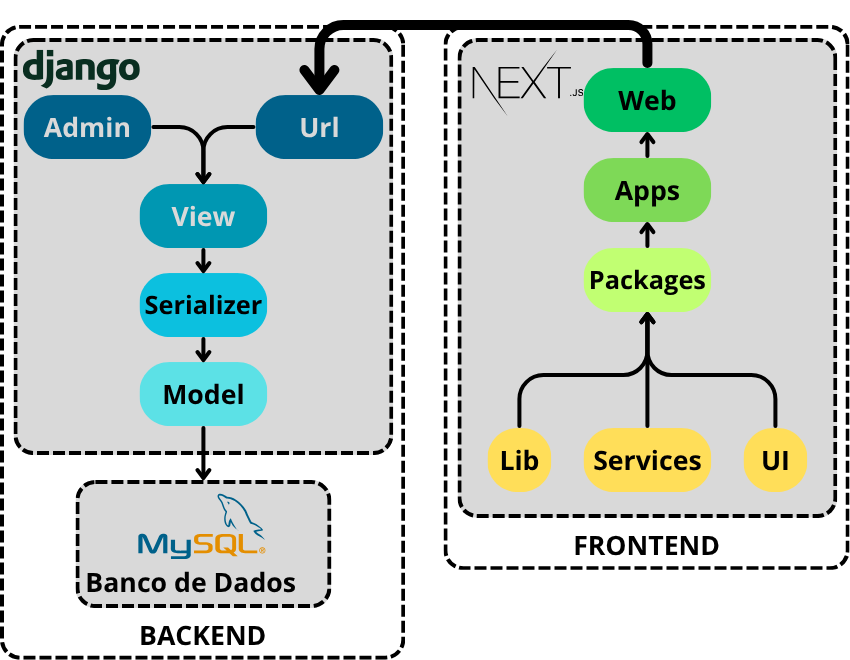
\includegraphics[width=0.70\textwidth]{figuras/Representacao_Arquitetura.png}


    Fonte: Autoria própria.
    
    \vspace{0.2cm}
        
    \label{fig:RepresentacaoArquitetura}
\end{figure}

\subsection [Backend Django]{Backend Django}
O \textit{backend} é responsável pela lógica de negócio, processamento de dados e persistência, seguindo a arquitetura MVS do Django, que promove uma clara separação de responsabilidades.

\textit{Model}: A camada \textit{Model} representa a estrutura dos dados da aplicação. Implementada através das \textit{Models} do Django, ela serve como a única fonte da verdade para os dados. Utilizando o ORM (\textit{Object-Relational Mapping}) integrado do Django, as classes Python são mapeadas diretamente para as tabelas no banco de dados MySQL neste projeto. Toda a lógica de acesso, validação e manipulação dos dados reside aqui.

\textit{View}: Na terminologia do Django, a \textit{View} atua como a \textit{Controller} do padrão MVC clássico. É a camada que processa as requisições HTTP (\textit{Hypertext Transfer Protocol}) recebidas do cliente. Ela contém a lógica de negócio, interage com a \textit{Model} para buscar ou modificar dados e retorna uma resposta HTTP. Para este projeto, será utilizado o \textit{Django Rest Framework} (DRF) para construir as \textit{Views}, que se tornam \textit{endpoints} de uma API, retornando respostas em formato JSON (\textit{JavaScript Object Notation}).

\textit{Serializer}: Esta camada corresponde à \textit{View} no padrão MVC. No contexto de uma API, a \textit{view} é uma representação serializada dos dados, geralmente em JSON. O DRF gerencia essa serialização, transformando os objetos complexos da \textit{Model} em um formato que o \textit{frontend} pode facilmente consumir.

Integradas a esta arquitetura, as bibliotecas \textit{Pandas} e \textit{Scikit-learn} são empregadas dentro da camada de lógica de negócio (nas \textit{Views} ou em módulos de serviço por elas invocados) para realizar análises de dados e executar modelos de \textit{machine learning} antes de os dados serem persistidos ou retornados ao cliente. O fluxo de dados no \textit{backend} é, portanto, unidirecional e bem definido: uma requisição chega a uma \textit{View}, que utiliza a \textit{Model} para interagir com o banco de dados e, por fim, formula uma resposta através de um serializador (\textit{Serializer}).

\subsection[Frontend Nextjs]{Frontend Nextjs}
Para o \textit{frontend} foi adotada uma arquitetura de \textit{Monorepo} (monorepositório), que consiste em gerenciar múltiplos projetos e pacotes em um único repositório de código. Esta abordagem é ideal para escalar a aplicação, promover o reuso de código e simplificar a gestão de dependências.

\textit{Web}: A aplicação principal desenvolvida com Next.js e React. Ela é responsável por toda a interface do usuário, gerenciamento de estado do cliente e consumo da API do \textit{backend}. O TypeScript é utilizado para garantir a segurança de tipos e o Prisma ORM  empregado para gerar tipos TypeScript a partir do esquema da API, garantindo a sincronia entre \textit{frontend} e \textit{backend}.

\textit{Packages}: Contém códigos que são compartilhados entre as diferentes páginas.

UI (\textit{User Interface}): Uma biblioteca de componentes React puros, estilizados com Tailwind CSS (\textit{Cascading Style Sheets}). Manter os componentes em um pacote separado permite seu reuso.

\textit{Config}: Centraliza as configurações de ferramentas de desenvolvimento, como ESLint e tsconfig.json (TypeScript), garantindo consistência em todo o repositório.

\textit{Lib}: Agrupa lógica compartilhada, como \textit{hooks} React customizados e funções de formatação de dados.

\textit{Services}: Agrupa funções que realizam requisições ao \textit{backend}.

Essa arquitetura permite que a interface do usuário seja construída de forma modular e consistente, além de otimizar o processo de \textit{build} e os fluxos de integração contínua.

\subsection [Interação entre Camadas e Tecnologias de Suporte]{Interação entre Camadas e Tecnologias de Suporte}

O MVS e o Monorepo operam de forma desacoplada. A comunicação entre eles é realizada exclusivamente através de uma API bem definida, com requisições HTTPS.

Docker: Toda a infraestrutura da aplicação é encapsulada em contêineres. Utiliza-se docker-compose para orquestrar contêineres separados para o \textit{backend} Django, o \textit{frontend} Next.js, o banco de dados MySQL e o \textit{proxy} reverso. Isso garante paridade entre os ambientes de desenvolvimento, teste e produção.

\section[Banco de Dados]{Banco de Dados}

\subsection[Diagrama Entidade-Relacionamento]{Diagrama Entidade-Relacionamento}

O Diagrama Entidade-Relacionamento (DE-R) é um diagrama que
representa as entidades do banco de dados (coisas que existem no mundo real e que se deseja armazenar dados), seus atributos (propriedades específicas que descrevem as entidades) e os relacionamentos que existem entre as entidades \cite{elmasri2011sistemas}.

No DE-R, as entidades são representadas por retângulos, os relacionamentos são representados por losangos (e geralmente descritos com um verbo) e atributos são representados por elipses, conectadas por linhas às suas entidades \cite{elmasri2011sistemas}. A Figura \ref{fig:diagrama_DE-R} apresenta o DE-R do projeto.

\clearpage

\begin{landscape}
    \begin{figure}
        \centering
        \caption{Diagrama Entidade-Relacionamento do projeto.} 
        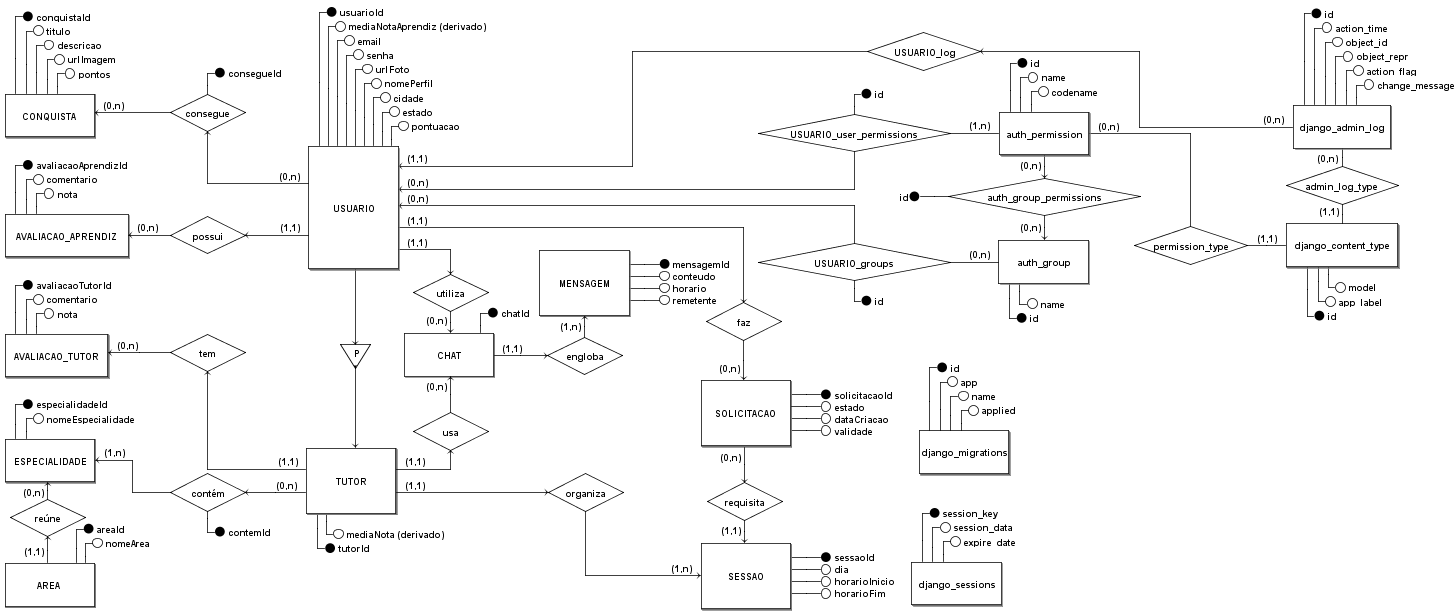
\includegraphics[width=1.5\textwidth, height=0.90\textheight, keepaspectratio]{figuras/DE-R.png}
    
    
        Fonte: Autoria própria.
        
        \vspace{0.2cm}
            
        \label{fig:diagrama_DE-R}
    \end{figure}
\end{landscape}

\clearpage

\subsection[Diagrama Lógico de Dados]{Diagrama Lógico de Dados}

O nível lógico de um projeto de banco de dados é uma descrição da base de dados que será implementada no Sistema Gerenciador de Banco de Dados (SGBD). Assim, cada entidade do banco é traduzida para uma tabela, e cada atributo, geralmente, define uma coluna desta tabela. Além disso, definem-se as chaves primárias e chaves estrangeiras,  os tipos de dados de cada coluna, dentre outros
recursos e restrições relevantes a base de dados que estará sendo implementada \cite{heuser2009projeto}. A Figura \ref{fig:diagrama_DLD} apresenta o Diagrama Lógico de Dados (DLD) do projeto.

Além do DLD e DE-R, foi criado um dicionário de dados da base de dados do software proposto. Um dicionário de dados é a descrição da base de dados, armazenando informações sobre sua estrutura e restrições \cite{elmasri2011sistemas}. No  Apêndice \ref{dicionario-dados} pode ser observado tal dicionário. 

\clearpage

\begin{landscape}
    \begin{figure}[h!]
        \centering
        \caption{Diagrama Lógico de Dados.} 
        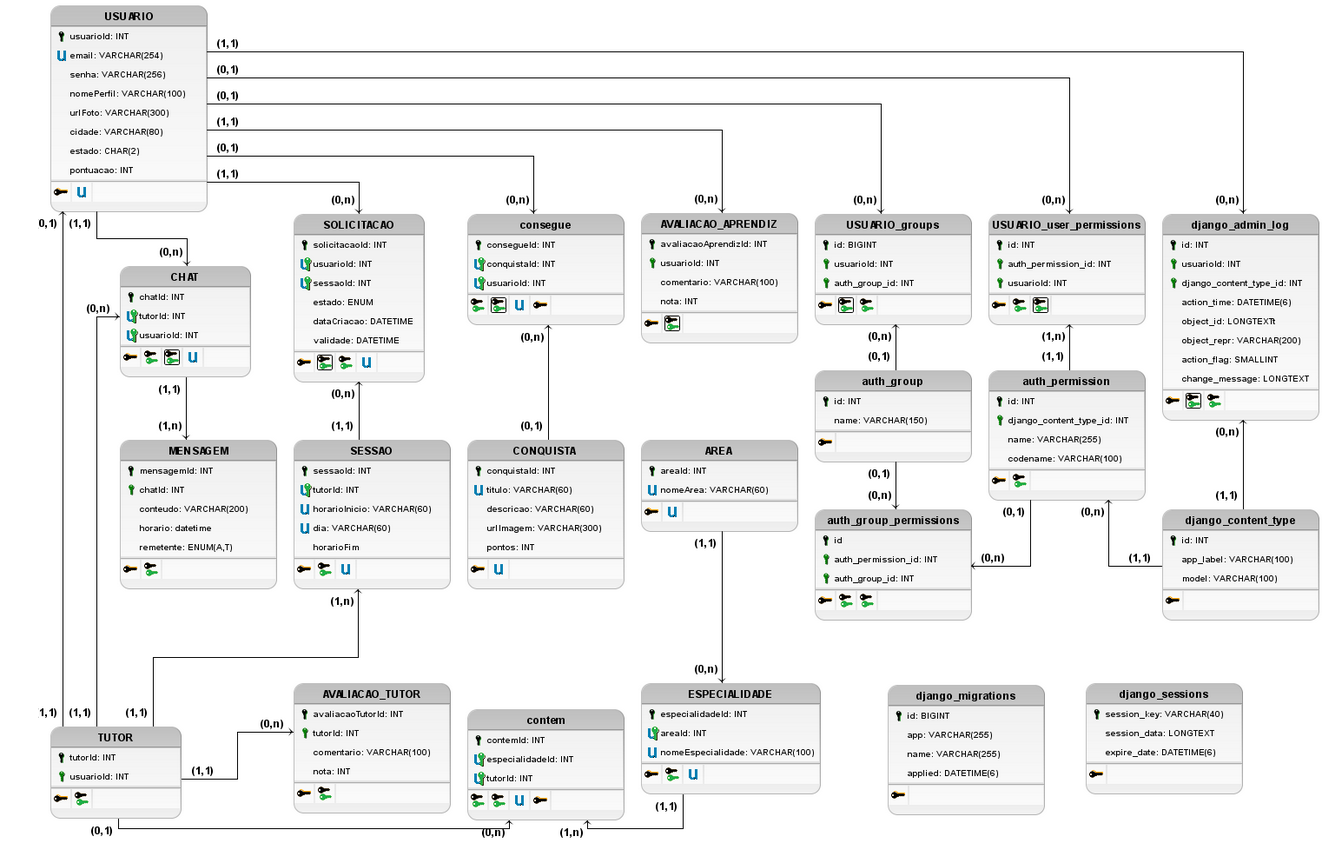
\includegraphics[width=1.5\textwidth, height=0.90\textheight, keepaspectratio]{figuras/DLD_print.png}
    
    
        Fonte: Autoria própria.
        
        \vspace{0.2cm}
            
        \label{fig:diagrama_DLD}
    \end{figure}
\end{landscape}

\clearpage

\section[Suporte Tecnológico]{Suporte Tecnológico}

Para auxiliar o processo de desenvolvimento deste projeto, foram utilizadas as ferramentas tecnológicas descritas a seguir:

\subsection[Git]{Git}
O Git é um sistema de controle de versão distribuído, gratuito e de código aberto, projetado para lidar com projetos de todos os tamanhos com velocidade e eficiência \cite{git2026}. O Git permite que cada desenvolvedor tenha uma cópia completa do histórico do projeto.

Neste trabalho, o Git foi utilizado para o versionamento de todo o código-fonte da simulação e do software, permitindo o controle das alterações e a integridade do trabalho desenvolvido.

\subsection[GitHub]{GitHub}
O GitHub é uma plataforma de hospedagem de código-fonte que utiliza o sistema Git para controle de versão, oferecendo também ferramentas de colaboração e gerenciamento de projetos \cite{github2026}. Ele atua como um ponto central para o armazenamento do repositório remoto.

No contexto deste projeto, o GitHub foi utilizado para hospedar os repositórios do \textit{frontend} e \textit{backend}, facilitando a colaboração entre os desenvolvedores e o acompanhamento das atualizações do código.

\subsection[brModelo]{brModelo}
O brModelo é uma ferramenta CASE (\textit{Computer-Aided Software Engineering}) de código aberto, voltada para o ensino e a modelagem de bancos de dados relacionais \cite{candido2020brmodelo}. Ela permite a criação de modelos conceituais e lógicos de maneira intuitiva.

Para este projeto, a ferramenta foi empregada na elaboração do DE-R e do DLD.

\subsection[Canva]{Canva}
O Canva é uma plataforma de design gráfico e comunicação visual online que oferece ferramentas para a criação de diversos tipos de conteúdos visuais, como apresentações, infográficos e diagramas \cite{canva2026}.

Neste trabalho, o Canva foi utilizado para a criação do diagrama ilustrativo da arquitetura do projeto.

\subsection[LaTeX e Overleaf]{LaTeX e Overleaf}

O LaTeX é um sistema de preparação de documentos de alta qualidade tipográfica, amplamente utilizado para a produção de documentação técnica e científica, facilitando a gestão de referências bibliográficas e fórmulas matemáticas \cite{latex2026}. O Overleaf, por sua vez, é uma ferramenta de edição e publicação colaborativa online baseada em LaTeX \cite{overleaf2026}.

A escolha dessas ferramentas para a escrita desta monografia deve-se à facilidade de formatação conforme as normas acadêmicas, à gestão automatizada de referências e à capacidade de edição simultânea e colaborativa do documento pelos autores.

\subsection[Discord]{Discord}
Um aplicativo de comunicação gratuito que permite conversas por voz, vídeo e texto \cite{pearson2025discord}. Foi utilizado para a realização de reuniões com compartilhamento de tela para discussões e desenvolvimento do trabalho.

\subsection[Telegram]{Telegram}
Aplicativo de mensagens gratuito baseado em nuvem com suporte a chamadas de voz e vídeo, além de compartilhamento de arquivos \cite{telegram2025}. Utilizado para comunicação, reuniões de acompanhamento de progresso entre os desenvolvedores e compartilhamento de arquivos.

\subsection[LucidChart]{LucidChart}
O Lucidchart é uma ferramenta baseada na web que auxilia usuários na criação e compartilhamento de fluxogramas, diagramas e mapas mentais profissionais de forma colaborativa \cite{lucidchart}. A plataforma permite a construção visual de processos complexos de maneira intuitiva.

Neste trabalho, o Lucidchart foi utilizado para a elaboração dos diagramas de fluxo de atividades dos processos metodológicos, permitindo a visualização clara das etapas de desenvolvimento do projeto.

\section[Processo Metodológico]{Processo Metodológico}

O Trabalho de Conclusão de Curso (TCC) em curso de Engenharia de Software na Universidade de Brasília (UnB) é realizado em duas etapas, denominadas TCC1 e TCC2. No TCC1 o objetivo é buscar o embasamento teórico necessário do projeto, bem como a elaboração de uma proposta de projeto. No TCC2 realiza-se a execução do planejamento elaborado na etapa anterior, consistindo no desenvolvimento completo das funcionalidades do software, na aplicação de testes e, por fim, na análise dos resultados alcançados para averiguar o êxito da solução proposta.

Com o propósito de definir e acompanhar o processo de desenvolvimento completo do TCC, foi modelado um processo metodológico para cada etapa, apresentados nas Seções \ref{sec:tcc1} e \ref{sec:tcc2}, além dos respectivos cronogramas com suas principais atividades.

\subsection[TCC1]{TCC1}
\label{sec:tcc1}

Nesta seção, é detalhado o processo metodológico adotado para a condução da primeira etapa do trabalho (TCC1). O fluxo de atividades realizadas é ilustrado na Figura \ref{fig:metodologiaTCC1}. A seguir, são descritas as atividades que compõem esse fluxo, bem como o cronograma de execução das atividades.

\begin{figure}[h!]
    \centering
    \caption{Metodologia para elaboração do TCC1.} 
    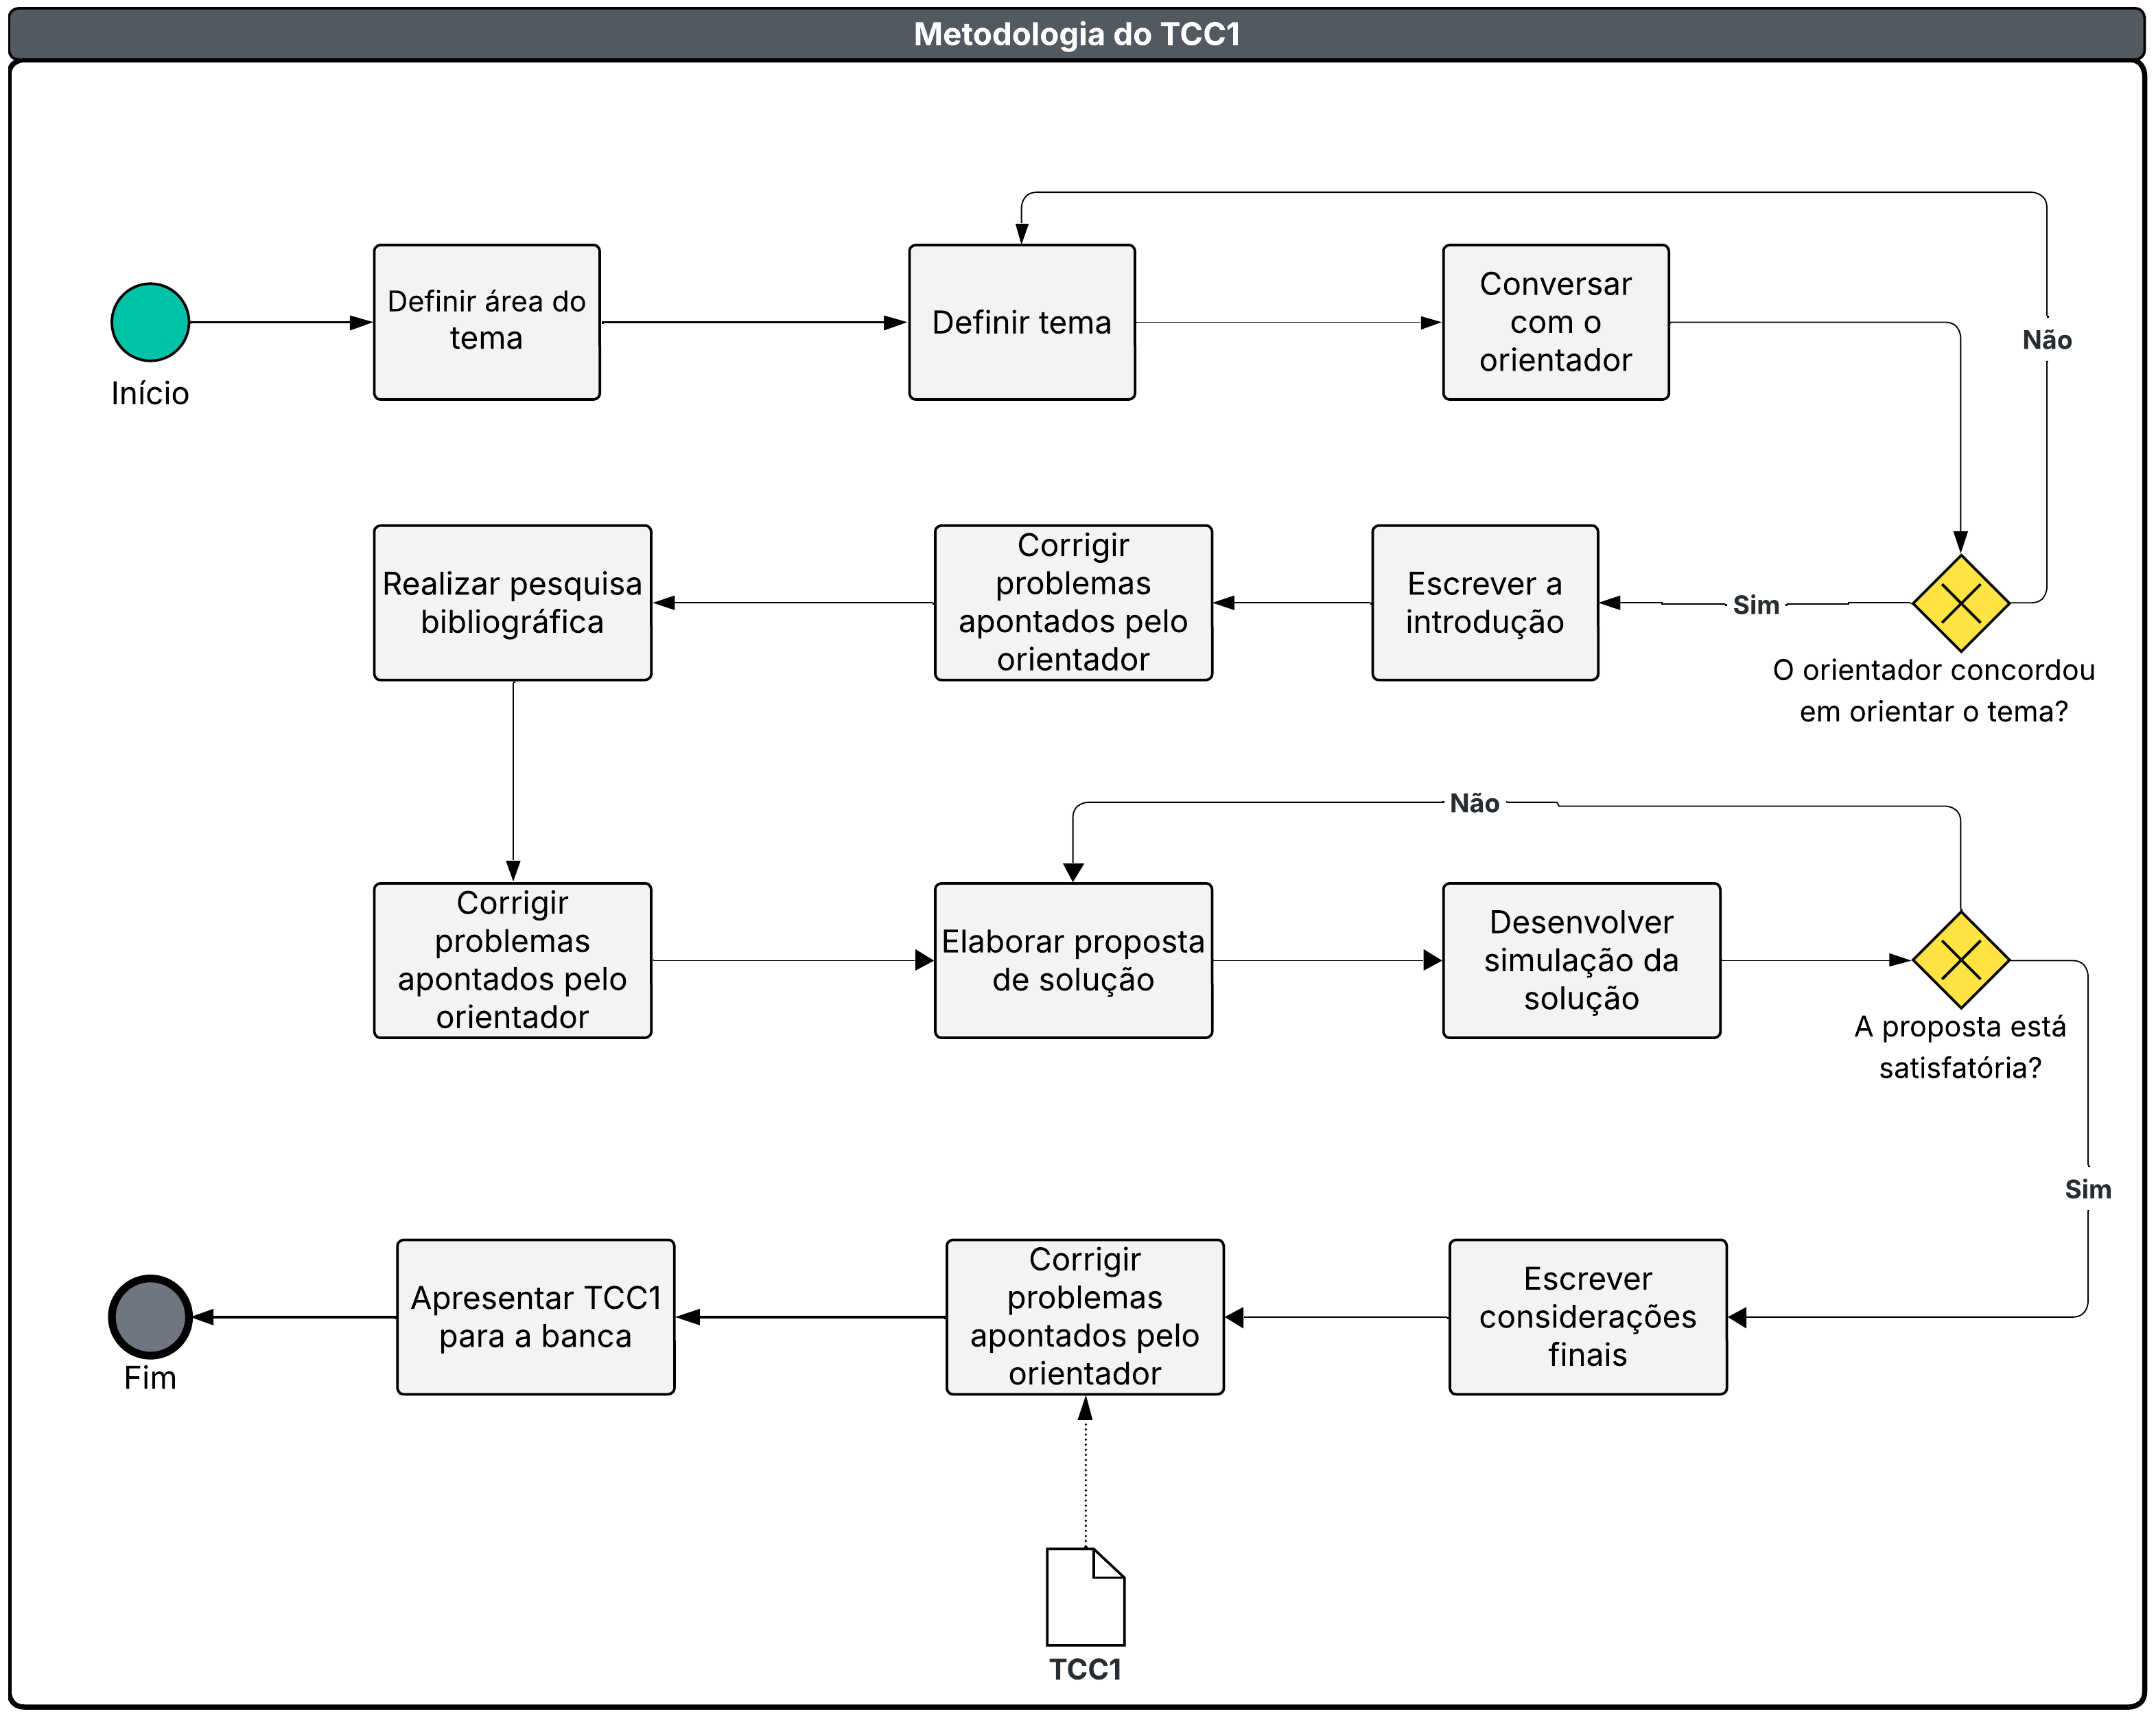
\includegraphics[width=0.87\textwidth]{figuras/diagrama_atividades_TCC1.png}


    Fonte: Autoria própria.
    
    \vspace{0.2cm}
        
    \label{fig:metodologiaTCC1}
\end{figure}

As atividades presentes na Figura \ref{fig:metodologiaTCC1} são descritas a seguir:

\begin{itemize}

\item \textbf{Definir área do tema}: definir qual área de Engenharia da Software será empregada no trabalho;

\item \textbf{Definir tema}: dentro da área escolhida, definir qual será o tema principal a ser desenvolvido no trabalho;

\item \textbf{Conversar com o orientador}: conversar com o orientador para validar o tema e verificar sua disponibilidade e interesse em orientar o trabalho proposto no TCC;

\item \textbf{Escrever a introdução}: detalhar o contexto do projeto proposto;

\item \textbf{Corrigir problemas apontados pelo orientador}: corrigir e evoluir todos os apontamentos indicados pelo orientador do trabalho;

\item \textbf{Realizar pesquisa bibliográfica}: pesquisar autores, artigos e publicações a respeito de temas relevantes para um melhor entendimento do trabalho trabalho e seu contexto;

\item \textbf{Elaborar proposta de solução}: apresentar a proposta de software a ser desenvolvida na primeira etapa do TCC;

\item \textbf{Desenvolver simulação da solução}: desenvolver parcialmente algumas funcionalidades do software proposto a fim de validar a viabilidade da arquitetura proposta, disponível no Apêndice X;

\item \textbf{Escrever considerações finais}: elaborar de maneira sucinta e objetiva o que foi alcançado com a proposta de trabalho (TCC1);

\item \textbf{Apresentar TCC1 para a banca}: realizar a apresentação da proposta para a banca examinadora.

\end{itemize}

\newpage

\subsubsection[Cronograma TCC1]{Cronograma TCC1}

\begin{table}[h!]
\centering
\caption{Cronograma com principais Atividades Previstas para o TCC1.}
\label{tab:cronograma-atividades-final}
\small 
\setlength{\tabcolsep}{4pt} 
\begin{tabular}{|l|c|c|c|c|c|c|c|c|c|c|c|c|}
\hline
\textbf{Atividade} & 
\rotatebox{90}{\textbf{Dezembro - 2024}} & 
\rotatebox{90}{\textbf{Janeiro - 2025}} & 
\rotatebox{90}{\textbf{Março - 2025}} & 
\rotatebox{90}{\textbf{Abril - 2025}} & 
\rotatebox{90}{\textbf{Maio - 2025}} & 
\rotatebox{90}{\textbf{Junho - 2025}} & 
\rotatebox{90}{\textbf{Julho - 2025}} & 
\rotatebox{90}{\textbf{Agosto - 2025}} & 
\rotatebox{90}{\textbf{Setembro - 2025}} &
\rotatebox{90}{\textbf{Outubro - 2025}} &
\rotatebox{90}{\textbf{Novembro - 2025}} &
\rotatebox{90}{\textbf{Dezembro - 2025}} \\
\hline \hline
\textbf{Definir área do tema} & X & & & & & & & & & & & \\ \hline
\textbf{Definir tema} & X & & & & & & & & & & & \\ \hline
\textbf{Conversar com o orientador} & X & & & & & & & & & & & \\ \hline
\textbf{Corrigir problemas apontados pelo orientador} & & & & & & X & X & & & & X & \\ \hline
\textbf{Escrever a introdução} & X & X & & & & & & & & & & \\ \hline
\textbf{Realizar pesquisa bibliográfica} & & & X & X & X & & & & & & & \\ \hline
\textbf{Elaborar proposta de solução} & & & & & & X & X & X & X & X & & \\ \hline
\textbf{Desenvolver simulação da solução} & & & & & & & & & & X & & \\ \hline
\textbf{Escrever considerações finais} & & & & & & & & & & & X & \\ \hline
\textbf{Apresentar TCC1 para a banca} & & & & & & & & & & & & X \\ \hline
\end{tabular}
\par
\vspace{2mm}
Fonte: Autoria própria.
\end{table}

Embora a disciplina de TCC1 seja prevista para um semestre letivo, a elaboração deste trabalho estendeu-se pelo período de um ano. Essa extensão de prazo foi necessária para permitir uma investigação bibliográfica mais exaustiva, visando consolidar um embasamento teórico robusto para os capítulos iniciais, diante da especificidade dos temas abordados. Adicionalmente, houve a necessidade de readequar o cronograma para conciliar o desenvolvimento da proposta com a carga acadêmica das demais disciplinas cursadas simultaneamente, garantindo assim a qualidade da entrega final.

\subsection[TCC2]{TCC2}
\label{sec:tcc2}

Nesta seção, é detalhado o processo metodológico adotado para o desenvolvimento da segunda etapa do trabalho (TCC2). O fluxo de atividades realizadas é ilustrado na Figura
\ref{fig:metodologiaTCC2}. A seguir, são descritas as atividades que compõem esse fluxo, bem como o cronograma elaborado para a execução das atividades e o plano de testes elaborado para o software desenvolvido.

\newpage

\begin{figure}[h!]
    \centering
    \caption{Metodologia para elaboração do TCC2.} 
    
    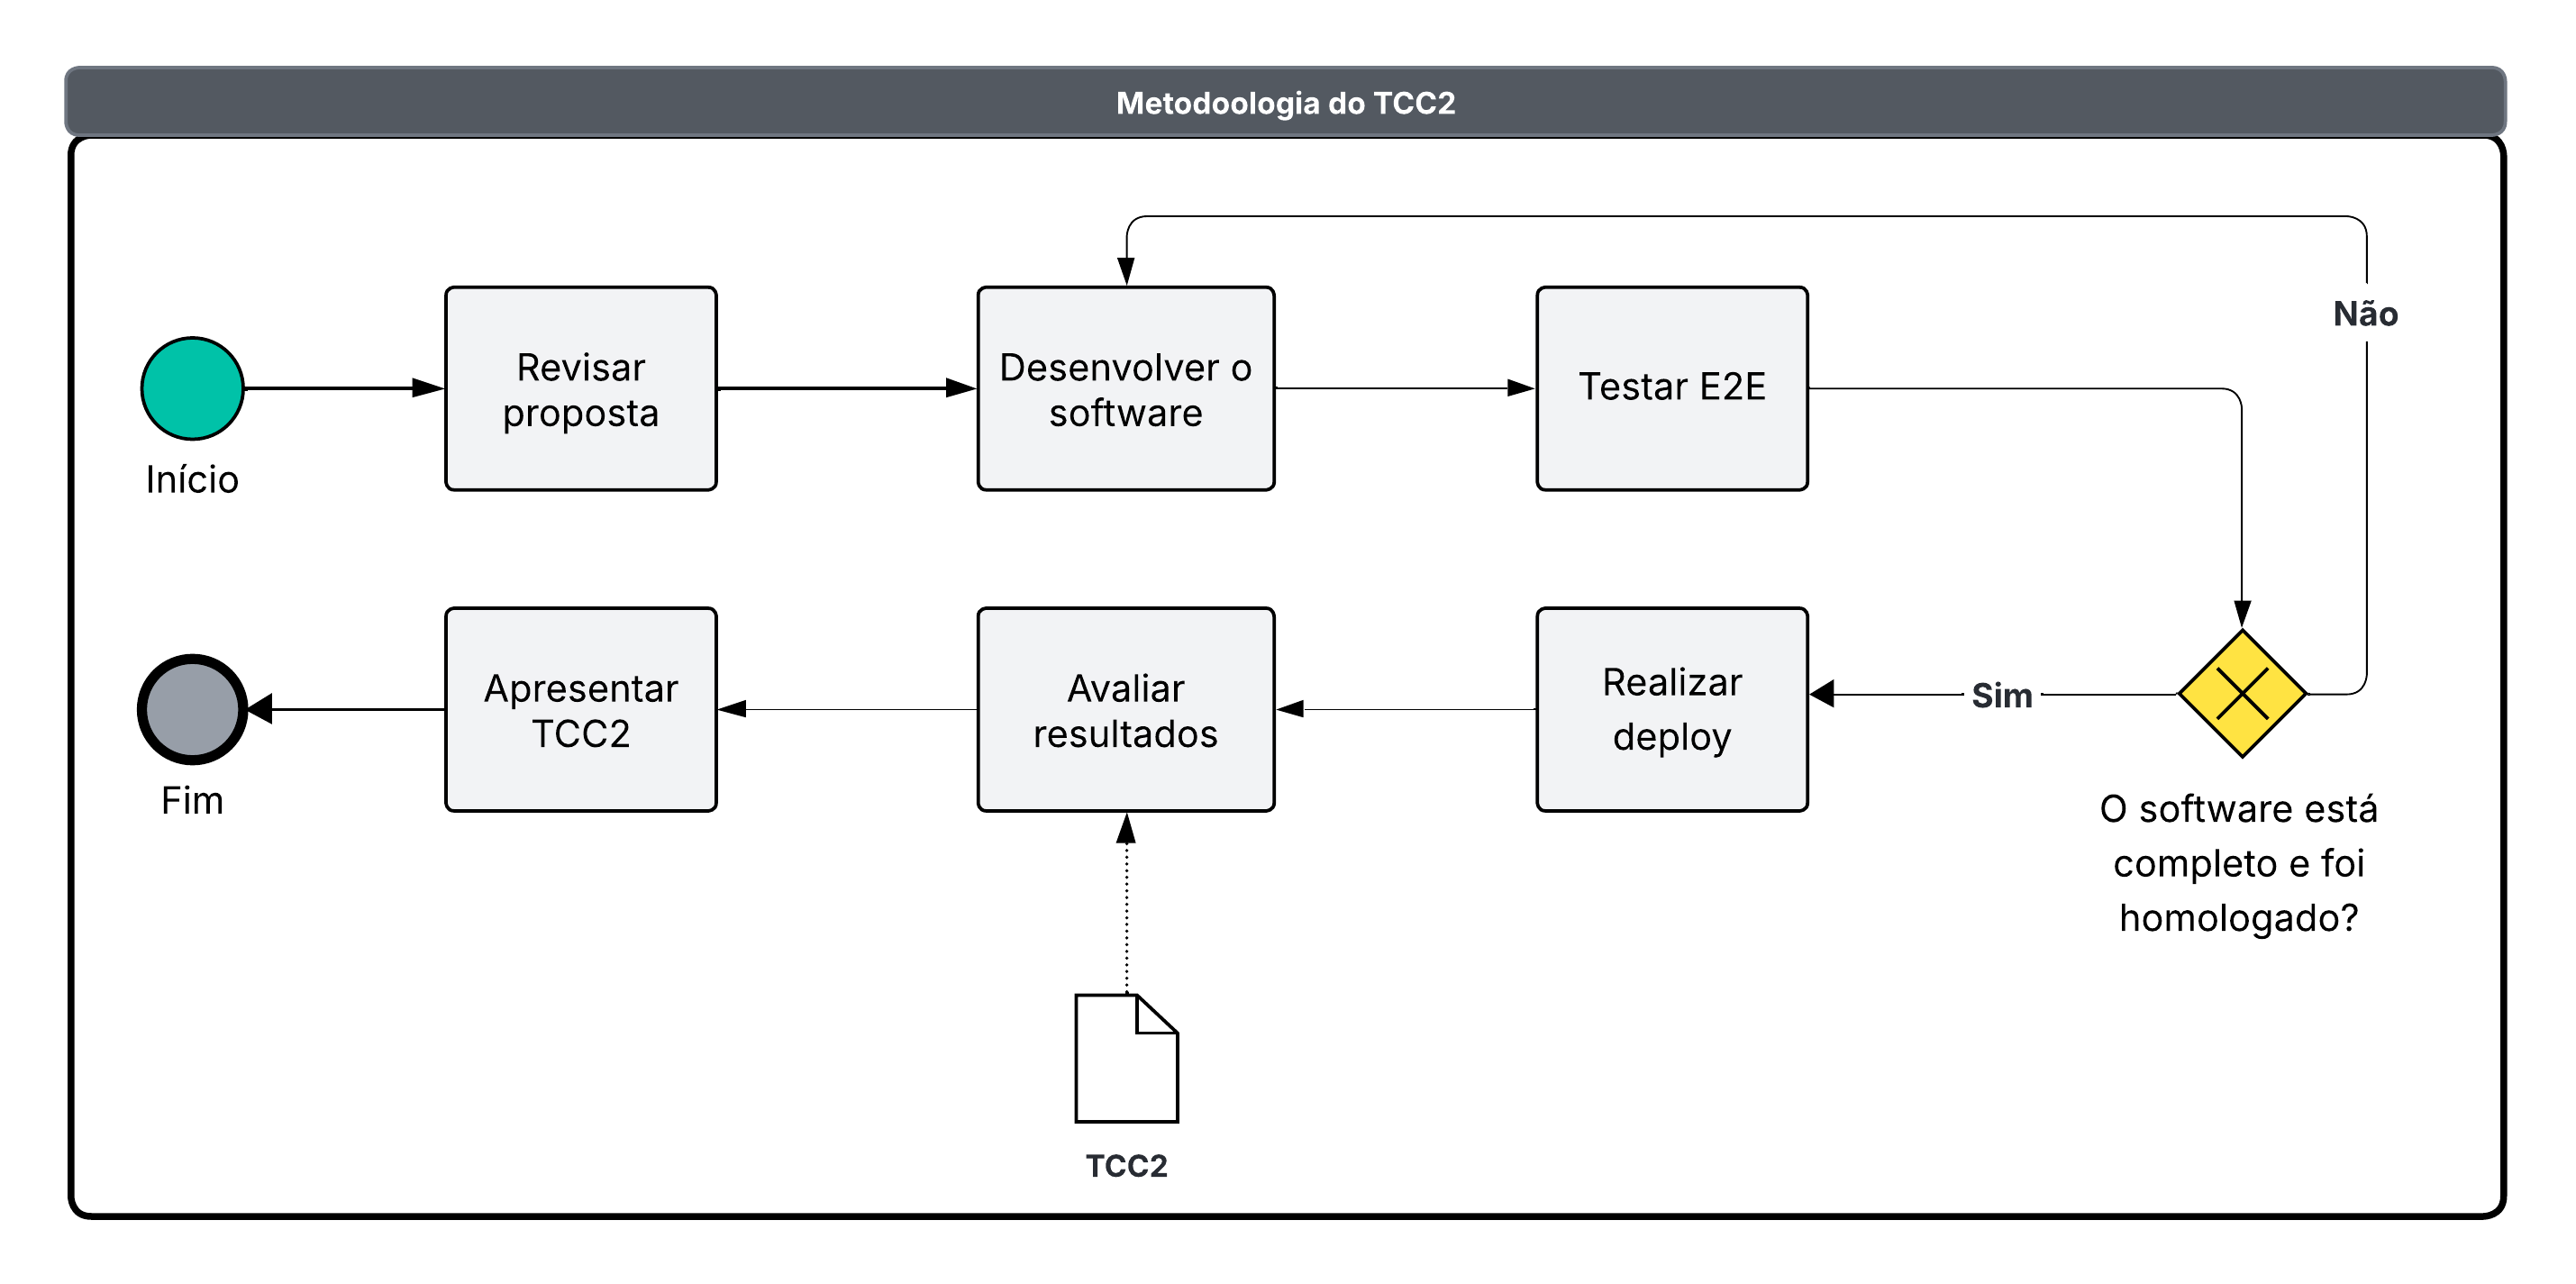
\includegraphics[width=0.90\textwidth]{figuras/diagrama_atividades_TCC2.png}
    
    \vspace{0.2cm}

    
    Fonte: Autoria própria.
    
    \label{fig:metodologiaTCC2}
\end{figure}

As atividades presentes na Figura \ref{fig:metodologiaTCC2} são descritas a seguir:

\begin{itemize}

\item \textbf{Revisar proposta}: realizar adições ou modificações no conteúdo do trabalho conforme o \textit{feedback} dos professores da banca avaliadora após a apresentação do TCC1;

\item \textbf{Desenvolver o software}: elaborar as funcionalidades do software seguindo a metodologia de desenvolvimento em conjunto com a realização de testes unitários e de integração conforme o plano de testes elaborado descrito na Subseção \ref{sec:PlanoDeTestes};

\item \textbf{Testar E2E}: realizar os testes End-to-End (E2E) para identificar inconsistências no fluxo de trabalho do usuário, visando a validação e homologação do software.

\item \textbf{Realizar \textit{deploy}}: realizar o \textit{deploy} do \textit{backend} e \textit{frontend} do software, possibilitando sua utilização pelos perfis de usuário através da Internet;

\item \textbf{Avaliar resultados}: analisar criticamente o software final desenvolvido, comparando os resultados alcançados com os objetivos propostos no trabalho e elaborar as conclusões finais do trabalho;

\item \textbf{Apresentar o TCC2}: realizar a apresentação do projeto para a banca examinadora.

\end{itemize}

\newpage

\subsubsection[Cronograma TCC2]{Cronograma TCC2}

\begin{table}[h!]
\centering
\caption{Cronograma de Atividades Previstas para o TCC2.}
\label{tab:cronograma-atividades-corrigido}
\small
\setlength{\tabcolsep}{4pt}
\begin{tabular}{|l|c|c|c|c|}
\hline
\textbf{Atividade} & \textbf{Março} & \textbf{Abril} & \textbf{Maio} & \textbf{Junho} \\ 
\hline \hline
Revisar proposta & X & & & \\ 
\hline
Desenvolver o software & X & X & X &  \\ 
\hline
Testar E2E & & & & X  \\ 
\hline
Realizar \textit{deploy} & & & & X  \\ 
\hline
Avaliar resultados & & & & X \\ 
\hline
Apresentar o TCC2 & & & & X \\ 
\hline
\end{tabular}
\par\vspace{2mm}
 Fonte: Autoria própria.
\end{table}

Conforme mencionado na subseção \ref{metodologia-desenvolvimento}, os ciclos de trabalho foram de uma semana. Sendo assim, as US listadas na subseção \ref{historias-usuario} estão distribuídas pelo cronograma da seguinte maneira:

\begin{itemize}

\item \textbf{Semana 1 (08-14 de Março)}: US01 (\textit{Login}) e US02 (Recuperar Senha);

\item \textbf{Semana 2 (15-21 de Março)}: US03 (Alterar Senha) e US04 (Alterar Informações);

\item \textbf{Semana 3 (22-28 de Março)}: US05 (Definir Agenda) e US06 (Gerenciar Especialidades).

\item \textbf{Semana 4 (29 de Março - 04 de Abril)}: US07 (Solicitar Horário);

\item \textbf{Semana 5 (05-11 de Abril)}: US08 (Aceitar e Recusar Solicitação) e US09 (Expirar Solicitação);

\item \textbf{Semana 6 (12-18 de Abril)}: US14 (Buscar Tutores);

\item \textbf{Semana 7 (19-25 de Abril)}: US10 (Avaliar Tutor);

\item \textbf{Semana 8 (26 de Abril - 02 de Maio)}: US11 (Avaliar Aprendiz) e US12 (Ver Reputação no Perfil);

\item \textbf{Semana 9 (03-09 de Maio)}: US13 (Enviar Mensagem);

\item \textbf{Semana 10 (10-16 de Maio)}: US15 (Recomendações);

\item \textbf{Semana 11 (17-23 de Maio)}: US16 (Conquistas);

\item \textbf{Semana 12 (24-30 de Maio)}: US17 (Níveis) e US18 (Títulos);

\end{itemize}

\subsubsection[Plano de Testes]{Plano de Testes}
\label{sec:PlanoDeTestes}

O plano de testes para o TCC 2 é realizar o TDD (do inglês \textit{Test Driven Development}, Desenvolvimento Orientado a Teste) com uma pirâmide de testes que abrange as funcionalidades descritas na Subseção \ref{historias-usuario}. A abordagem escolhida para o TDD é a Comportamental, que foca a validação apenas nos métodos públicos e fluxos principais. 

O projeto priorizou a validação por comportamento, assegurando que os testes cubram as regras de negócio relevantes e contratos de interface, evitando o acoplamento excessivo aos detalhes de implementação interna.

Os testes contemplam os níveis de teste unitário, teste de integração e teste E2E, que serão descritos a seguir:

\begin{itemize}

\item \textbf{Teste Unitários}: Técnica de teste automatizado que verifica as menores partes de um código, como funções ou métodos, isoladamente. O projeto tem uma cobertura de código de 70\% de testes unitários.

\item \textbf{Testes de Integração}: Utilizando abordagem ampla e \textit{Top-Down} de teste de integração, que inicia a validação na camada de interface mais alta (API/\textit{Endpoints}) e segue hierarquicamente até as camadas inferiores de infraestrutura e persistência.

O objetivo é simular o comportamento real de consumo do serviço, garantindo que a comunicação flua corretamente desde a entrada da requisição até a resposta dos componentes externos reais, validando a integridade da pilha completa de execução.

% Verifica a comunicação e a interação entre diferentes módulos ou componentes de um software, combinando-os para garantir que funcionem corretamente juntos. Serão executados testes de integração em todos os endpoints. Os testes unitários serão responsáveis por guiar o design da arquitetura interna, validando a existência de classes, métodos e regras de negócio. Enquanto os testes de integração focarão na validação dos \textit{endpoints} das funcionalidades, assegurando que os contratos da API e o fluxo de dados entre os componentes respondam corretamente às requisições.

\item \textbf{Teste E2E}: Simula o fluxo de trabalho de um usuário real com o sistema desenvolvido, para validar a aplicação do início ao fim, garantindo que todos os componentes integrados funcionem corretamente juntos. Foram aplicados testes E2E nas páginas em que haja interação com o usuário, evitando-se as páginas de somente exibição de texto.

\end{itemize}

\subsubsubsection[Ferramentas de Teste]{Ferramentas de Teste}
\begin{itemize}
    \item \textbf{POSTMAN}: Ferramenta para realização de testes de API.
    \item \textbf{DjangoUnit}: \textit{Framework} Python utilizado para teste unitários na \textit{Framework} Django.
    \item \textbf{Robot}: \textit{Framework} Python utilizada para testes E2E em aplicações web.
\end{itemize}

\subsubsubsection[Classificação de Bugs]{Classificação de Bugs}
Os \textit{bugs} estão classificados com as seguintes severidades descritas na Tabela \ref{tab:classificacao-bugs}.

\newpage

\begin{table}[h!]
    \centering
    \caption{Classificação dos \textit{Bugs}.}
    \label{tab:classificacao-bugs}
    % Define a tabela para ocupar 100% da largura da linha (\linewidth)
    % A coluna X se ajusta automaticamente para preencher o espaço restante
    \begin{tabularx}{\linewidth}{|c|l|X|}
        \hline
        \textbf{ID} & \textbf{Nível de Severidade} & \textbf{Descrição} \\
        \hline
        1 & Pequena & 
        \begin{itemize}
            \item Quase nenhum impacto na funcionalidade, porém atrapalha a experiência do usuário.
            \item Pequenos erros de interface do usuário.
            \item Erro ortográfico.
        \end{itemize}
        \\
        \hline
        2 & Moderada & 
        \begin{itemize}
            \item Funcionalidade não atinge certos critérios de aceitação, mas não compromete sua funcionalidade em geral.
        \end{itemize}
        \\
        \hline
        3 & Grave &
        \begin{itemize}
            \item Funcionalidade não funciona como o esperado.
            \item Interação de usuário incomum causa efeitos irreversíveis e prejudiciais.
        \end{itemize}
        \\
        \hline
        4 & Severa &
        \begin{itemize}
            \item Bug que bloqueia o teste de uma função ou causa falha na aplicação.
            \item Redirecionamento de página ou eventos de botão que impedem o uso da funcionalidade.
        \end{itemize}
        \\
        \hline
    \end{tabularx}
    \vspace{0.2cm} % Um pequeno espaço antes da fonte
    
    Fonte: Autoria Própria.
\end{table}

\subsubsubsection[Definição de Pronto]{Definição de Pronto}
Foi considerada pronta a funcionalidade que passou pela verificação de testes descrita e não apresentou \textit{bugs} com  severidade acima de Pequena ou não existiu \textit{bug} para esta funcionalidade.
% \chapter[Desenvolvimento]{Desenvolvimento}
\label{cap:desenvolvimento}

O objetivo deste trabalho é o desenvolvimento de uma aplicação web que possibilite o contato e agendamento de sessões entre tutores e aprendizes que precisem de tutoria em uma ou mais áreas de conhecimento, contando com um sistema de recomendação de tutores à aprendizes, empregando elementos de gamificação para manter os usuários mais engajados no uso do software proposto por este trabalho.

A pesquisa bibliográfica realizada permitiu o embasamento teórico e o melhor
entendimento do contexto do projeto: a aprendizagem colaborativa por tutoria, o potencial dos sistemas de recomendação híbridos e a aplicação de gamificação para o engajamento de usuários. A definição da metodologia de pesquisa (pesquisa aplicada e exploratória) permitiu a estruturação das necessidades e a elicitação dos requisitos por meio de métodos de identificação dos personas e as histórias de usuário. Com isso, foi possível delimitar o escopo e definir as metodologias de desenvolvimento ágil (XP e \textit{Kanban}) que guiarão a implementação de toda a proposta apresentada neste trabalho (TCC1).

Para a validação da arquitetura proposta, foram parcialmente implementadas três histórias de usuário em uma simulação simples. Diante do sucesso da simulação, foi demonstrada a viabilidade da execução do projeto para as demais funcionalidades a serem desenvolvidas no decorrer da próxima etapa do projeto (TCC2).

Portanto, a proposta de software apresentada neste trabalho poderá auxiliar aprendizes a encontrarem tutores para lhes auxiliarem em seus aprendizados, além de possibilitarem aos tutores expandirem sua clientela ou público-alvo, contribuindo para mitigação de problemas de aprendizagem de estudantes brasileiros em diferentes áreas de conhecimento envolvendo interesses pessoais ou profissionais.
%\input{editaveis/aspectosgerais}
%\input{editaveis/consideracoes}

% --------- MANTENHA COMENTADO
% \input{editaveis/textoepostexto}
% \input{editaveis/elementosdotexto}
% \input{editaveis/elementosdopostexto}

\bookmarksetup{startatroot} 

\postextual

\bibliography{bibliografia}

% ---------- DESCOMENTE APENDICE
\begin{apendicesenv}

% \partanexos

\chapter{Personas}
\label{personas}

\section{Persona 1}

\textbf{Perfil e Fatos Concretos}

Carlos Eduardo é um estudante universitário de 25 anos. Ele mora com a família em um pequeno apartamento no Gama, Distrito Federal. Além da universidade, também é estagiário de uma pequena empresa da região, o que deixa sua rotina com pouco tempo livre. 

\textbf{Comportamento e Hábitos}

Carlos é uma pessoa muito esforçada e que se empenha no que faz. Entretanto, seu déficit de atenção, impaciência e uma ocasional procrastinação são obstáculos que o atrapalham, principalmente nos estudos. Para relaxar, ele gosta de jogar videogame, passar tempo com os amigos e fazer caminhada ao ar livre. Também gosta de ver vídeos curtos e usar redes sociais, como Instagram e Facebook. Possui forte interesse em atividades artísticas, possuindo o objetivo pessoal de aprender a tocar violão.

\textbf{Objetivos e Necessidades}

\begin{itemize}
\item \textbf{Objetivo Principal}: Aprender a tocar violão de forma consistente e com progresso visível.

\item \textbf{Necessidades}:

\begin{itemize}

\item \textbf{Acompanhamento Personalizado}: Precisa de alguém que possa dar \textit{feedback} direto e corrigir erros práticos (como a posição das mãos ao tocar o
violão).

\item \textbf{Flexibilidade de Horários}: Por ter uma agenda muito ocupada, precisa que suas aulam possam ser marcadas em horários específicos, geralmente à noite.

\item \textbf{Indicação de Confiança}: Precisa de uma fonte confiável para encontrar um professor confiável e competente, pois não possui indicações de amigos ou familiares.

\end{itemize}

\end{itemize}

\textbf{Frustrações}

Carlos se frustra muito com a falta de interação humana durante seu aprendizado de violão. No pouco tempo livre que possui à noite, ele tenta se dedicar ao \textit{hobby} através de cursos e vídeos online, mas não sente que está progredindo, se sentindo paralisado por dúvidas simples que os materiais gravados não conseguem sanar, como o posicionamento correto das mãos no instrumento musical.

Ele sente falta de ter alguém para tirar dúvidas pontuais e receber orientação personalizada, mas não conhece pessoalmente ninguém que possa ensiná-lo e não tem indicações de escolas de música ou tutores particulares em sua região.

\textbf{Familiaridade com Tecnologia}

Carlos é capaz de utilizar seu celular e computador diariamente sem nenhum problema. Está acostumado a usar redes sociais para comunicação e consome conteúdo em plataformas de vídeo. Além disso, está acostumado a usar plataformas de videochamada, como Google Meets e Microsoft Teams, visto que as usa frequentemente para realizar trabalhos da faculdade, sentindo-se confortável com interações e reuniões em ambiente online.

\newpage

\section{Persona 2}

\textbf{Perfil e Fatos Concretos}

Ricardo Almeida tem 38 anos, é casado e professor de música na Escola de Música de Brasília. Apaixonado por sua profissão, ele encontra grande satisfação em lecionar. Para complementar o orçamento da família,  ele oferece aulas particulares de violão e de guitarra durante a noite e fins de semana.

\textbf{Comportamento e Hábitos}

Como professor, Ricardo é muito paciente, didático e dedicado. Ele acredita que qualquer pessoa pode aprender música com o método e o incentivo certos, ficando muito feliz ao ver o progresso de seus alunos. Embora seja excelente em ensinar, Ricardo possui muita dificuldade em se promover com marketing digital nas redes sociais.

\textbf{Objetivos e Necessidades}

\begin{itemize}
\item \textbf{Objetivo Principal}: Aumentar sua base de alunos particulares para aumentar sua renda mensal e ter mais segurança financeira.

\item \textbf{Necessidades}:

\begin{itemize}

\item \textbf{Maior Visibilidade}: Precisa de uma forma de alcançar pessoas que estão procurando por aulas de música, em vez de tentar a sorte com o público geral das redes sociais.

\item \textbf{Ser Recomendado}: Deseja um espaço para construir uma reputação sólida baseada em sua experiência e nas avaliações de alunos, algo que pareça mais convincente que um perfil de Instagram.

\item \textbf{Gestão Simplificada}: Necessita de uma ferramenta para organizar seus horários e agendamentos de forma simples, sem depender de inúmeras trocas de mensagens pelo WhatsApp.

\end{itemize}

\end{itemize}

\textbf{Frustrações}

A principal frustração de Ricardo é a dificuldade em encontrar novos alunos. Atualmente, sua única forma de divulgação é um perfil no Instagram, onde ele posta vídeos tocando instrumentos musicais oferecendo dicas. Entretanto, se sente desmotivado com o baixo alcance de suas publicações, percebendo que a rede social promove perfis de entretenimento e grandes influenciadores, enquanto seu conteúdo, mais técnico e didático, raramente chega a potenciais clientes.

Ele sabe que é um bom professor, mas sente que não consegue a visibilidade que precisa para conseguir novos aprendizes. Além da dificuldade de divulgação, o processo de agendamento é manual e caótico, dependendo de conversas no WhatsApp que muitas vezes se estendem por dias e não resultam em uma aula de fato.

\textbf{Familiaridade com Tecnologia}

Ricardo é familiarizado com aplicativos e redes sociais, usando constantemente o WhatsApp e o Instagram para comunicação. Utiliza o Zoom e Google Meets para realizar suas aulas online. Sua dificuldade não está em usar essas ferramentas, mas em utilizá-las para marketing e obtenção de novos clientes de forma eficaz.

\chapter{Simulação da Arquitetura}
\label{simulacao}

Com o objetivo de verificação da viabilidade da arquitetura proposta na Seção \ref{arquitetura}, foi realizada uma simulação envolvendo alguns casos de uso da proposta do software. Nesta simulação foram realizadas as conexões entre o \textit{backend}, \textit{frontend} e o banco de dados, bem como a geração das imagens Docker e orquestração com Docker Compose.

A simulação consistiu em satisfazer parcialmente as histórias de usuário US01 (\textit{Login}), US07 (Solicitar Horário) e US16 (Conquistas).

A Figura \ref{fig:login} apresenta a interface de usuário para a ação do \textit{login}, em que é possível ver os campos destinados para o preenchimento de e-mail e senha para autenticação. Caso haja falha na autenticação, é exibida uma mensagem de erro para o usuário, advinda do \textit{backend} e tratada no \textit{frontend}, conforme apresentado na Figura \ref{fig:login-erro}.

\begin{figure}[h!]
    \centering
    \caption{Interface de \textit{login}.} 
    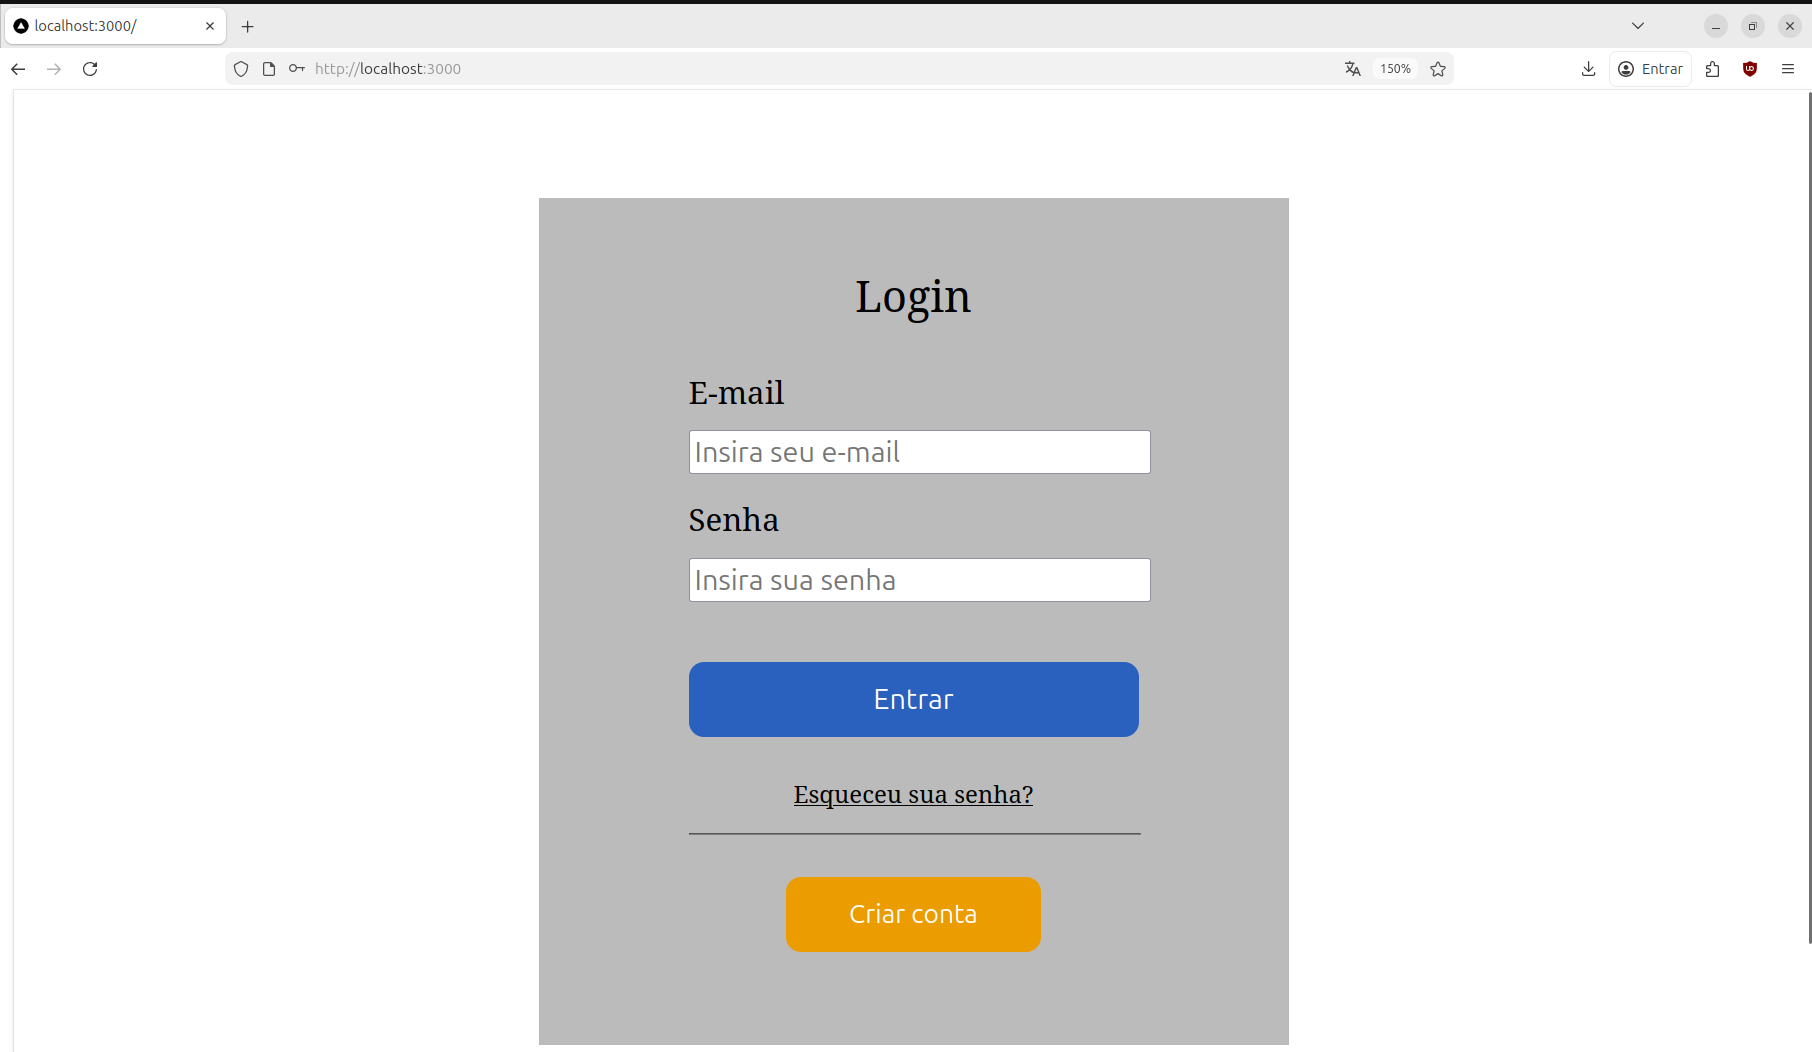
\includegraphics[width=0.99\textwidth]{figuras/login.png}
    
    Fonte: Autoria própria.
    
    \vspace{0.2cm}
        
    \label{fig:login}
\end{figure}

\begin{figure}[h!]
    \centering
    \caption{Mensagem de erro de autenticacação.} 
    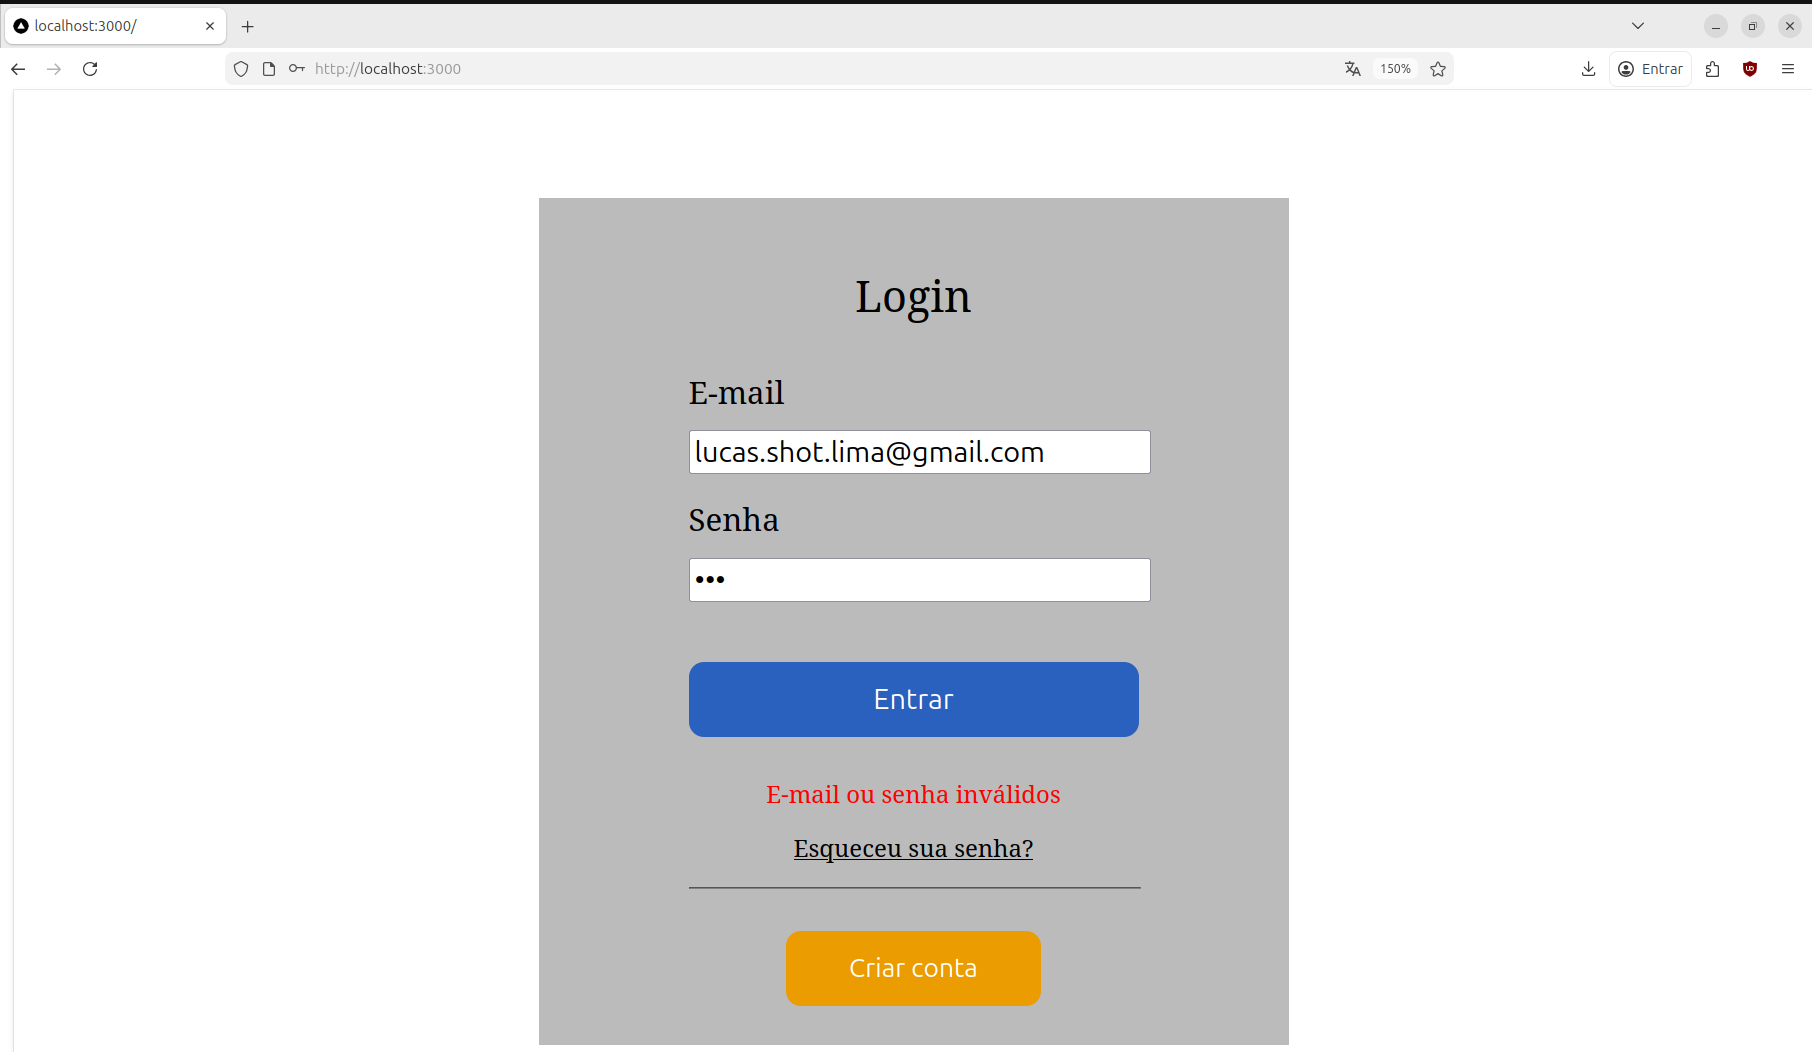
\includegraphics[width=0.99\textwidth]{figuras/login-erro.png}


    Fonte: Autoria própria.
    
    \vspace{0.2cm}
        
    \label{fig:login-erro}
\end{figure}

\newpage

A Figura \ref{fig:conquistas-bloqueadas} apresenta a tela de conquistas, a qual mostra a lista de conquistas com título, descrição, imagem e a pontuação fornecida ao usuário caso ele a desbloqueie. Conquistas bloqueadas são apresentadas com foto e texto em tom de cinza.

\begin{figure}[h!]
    \centering
    \caption{Lista de conquistas.} 
    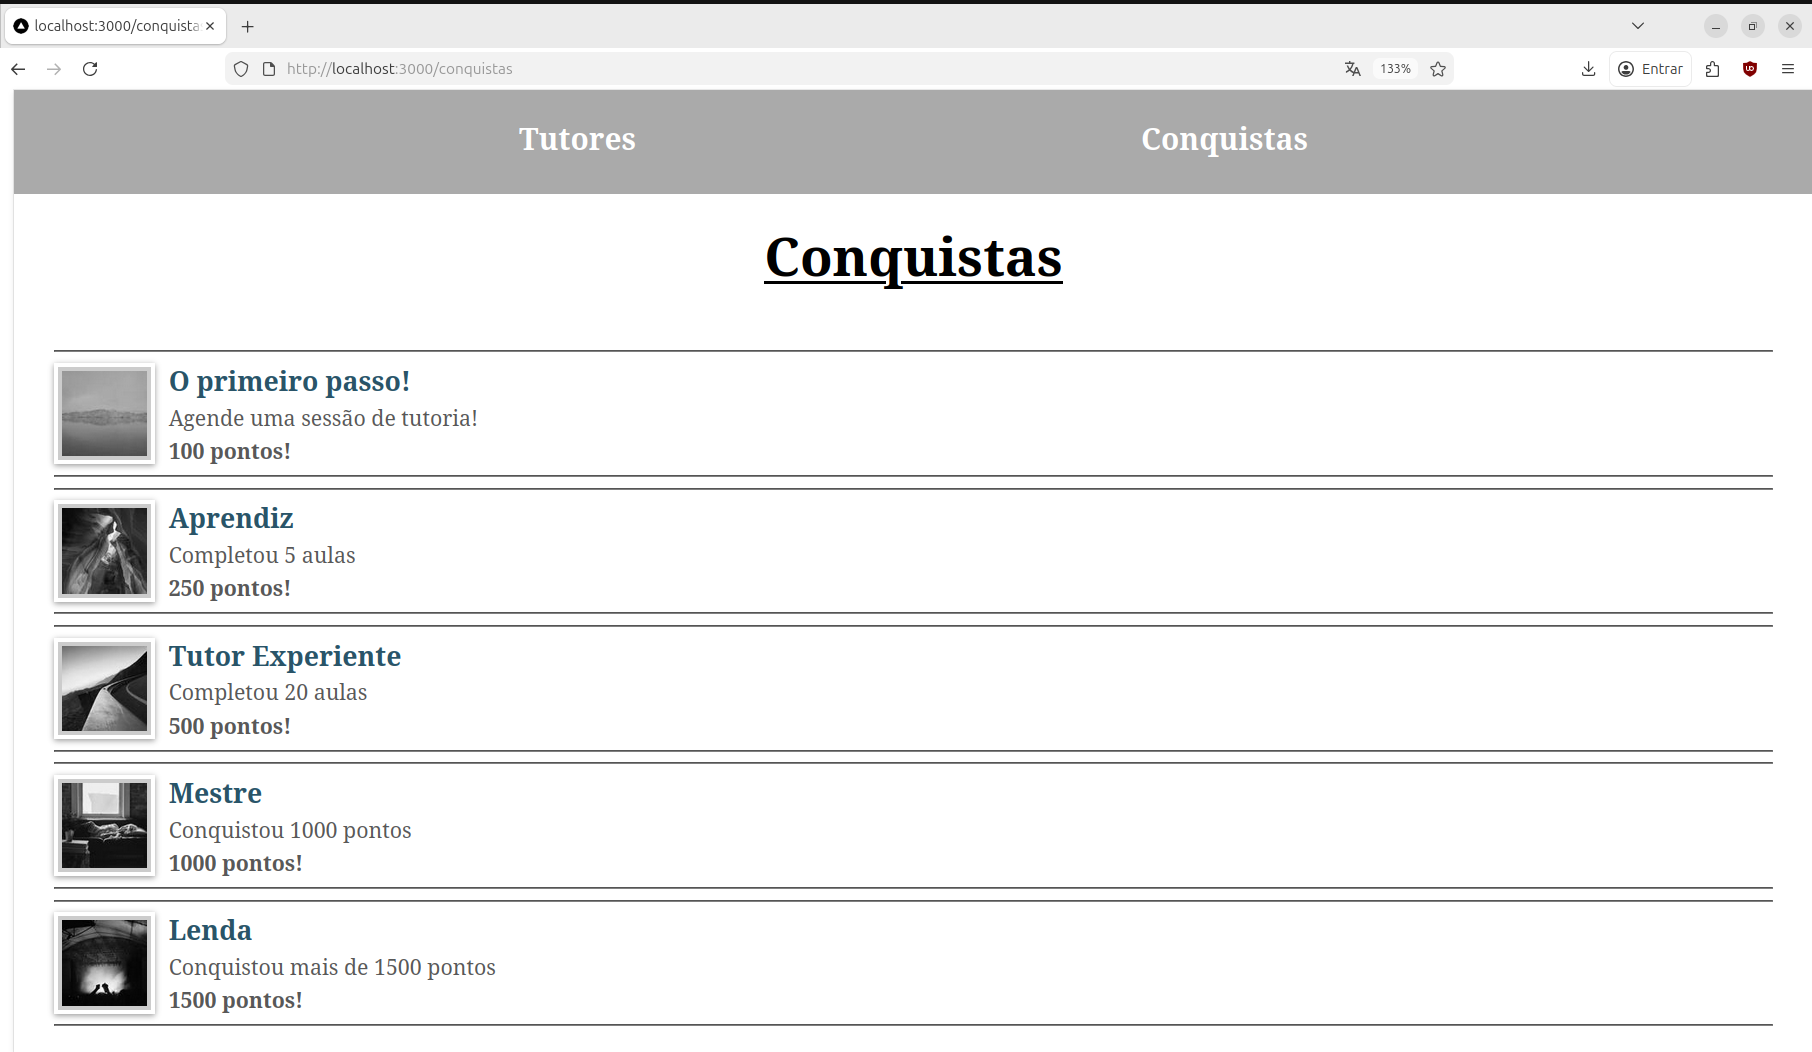
\includegraphics[width=0.99\textwidth]{figuras/conquistas-bloqueadas.png}


    Fonte: Autoria própria.
    
    \vspace{0.2cm}
        
    \label{fig:conquistas-bloqueadas}
\end{figure}

A Figura \ref{fig:tutores} apresenta a tela de tutores, que exibe tutores e suas informações, como nome, foto e áreas de conhecimento, além de dois botões interativos para o aprendiz acessar o perfil do tutor e também para solicitar uma sessão de tutoria.

\begin{figure}[h!]
    \centering
    \caption{Lista de tutores.} 
    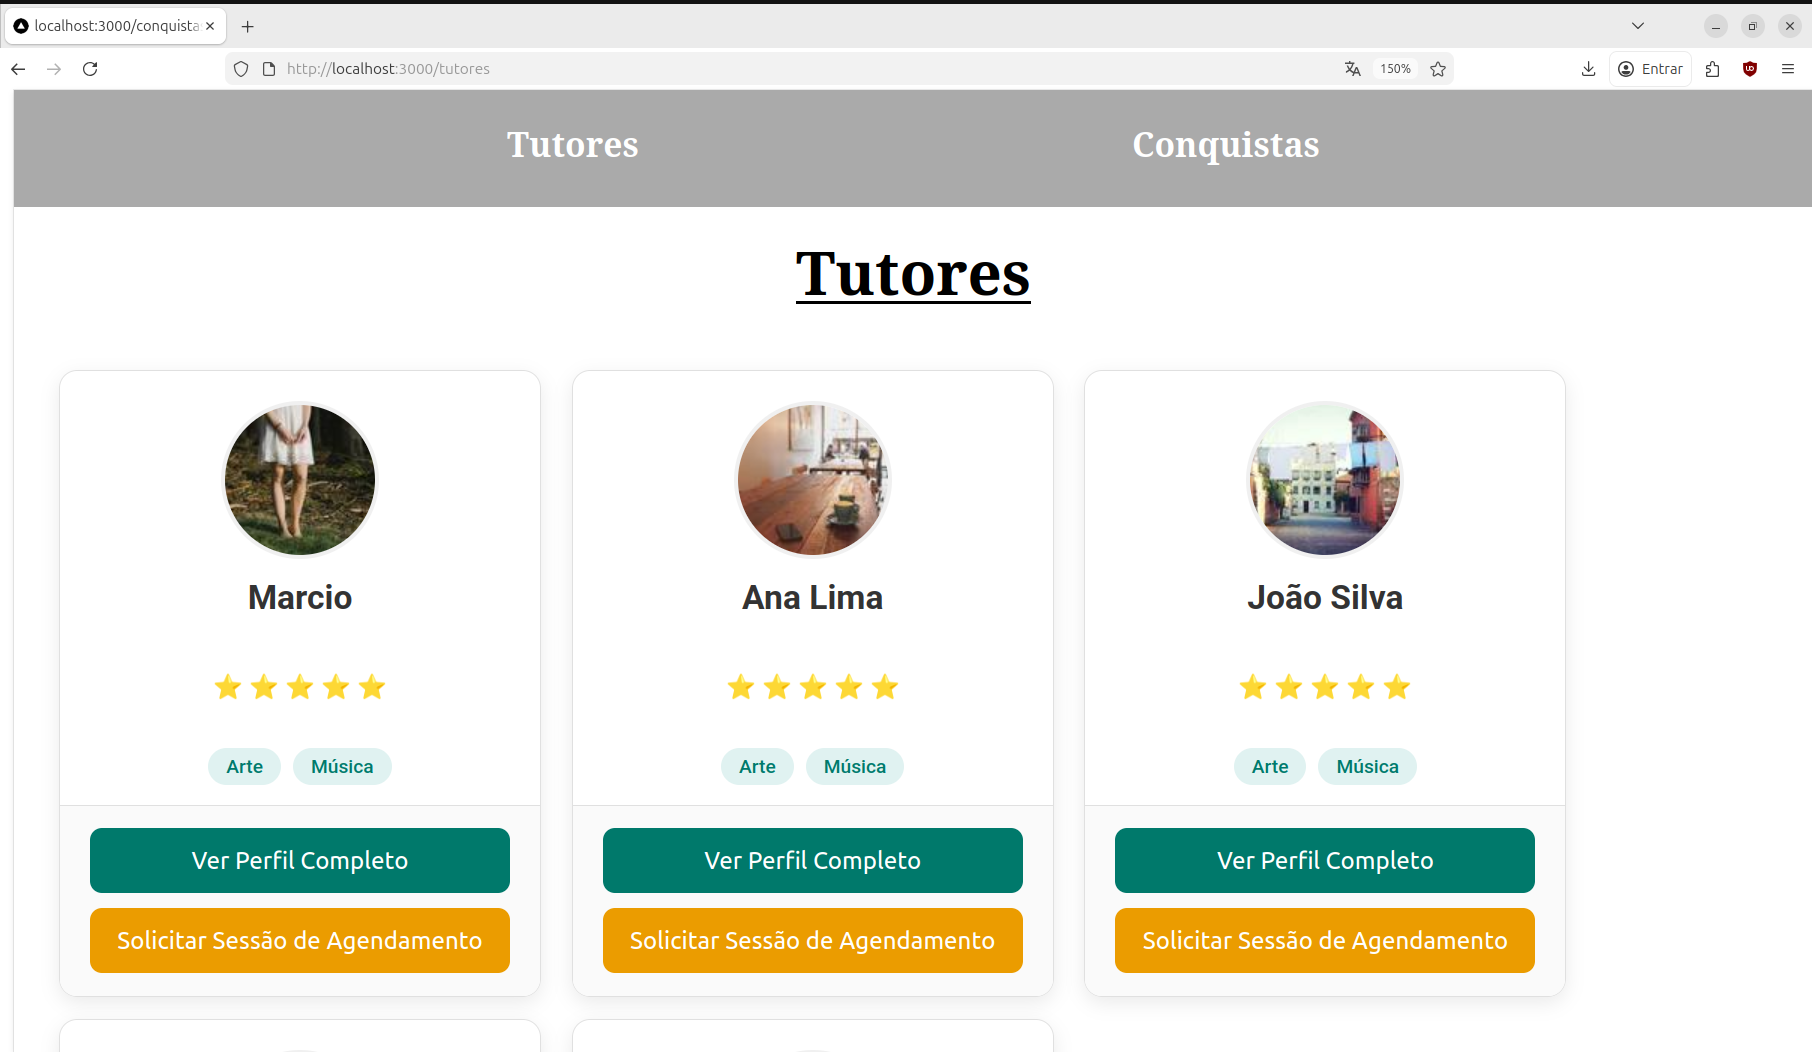
\includegraphics[width=0.99\textwidth]{figuras/tela-tutores.png}


    Fonte: Autoria própria.
    
    \vspace{0.2cm}
        
    \label{fig:tutores}
\end{figure}

Ao clicar no botão para solicitar uma sessão, abre-se uma janela em que são exibidos os horários disponíveis na agenda do tutor, conforme aprensentado pela Figura \ref{fig:sessoes}.

\newpage

\begin{figure}[h!]
    \centering
    \caption{Interface de agendamento da sessão de tutoria.} 
    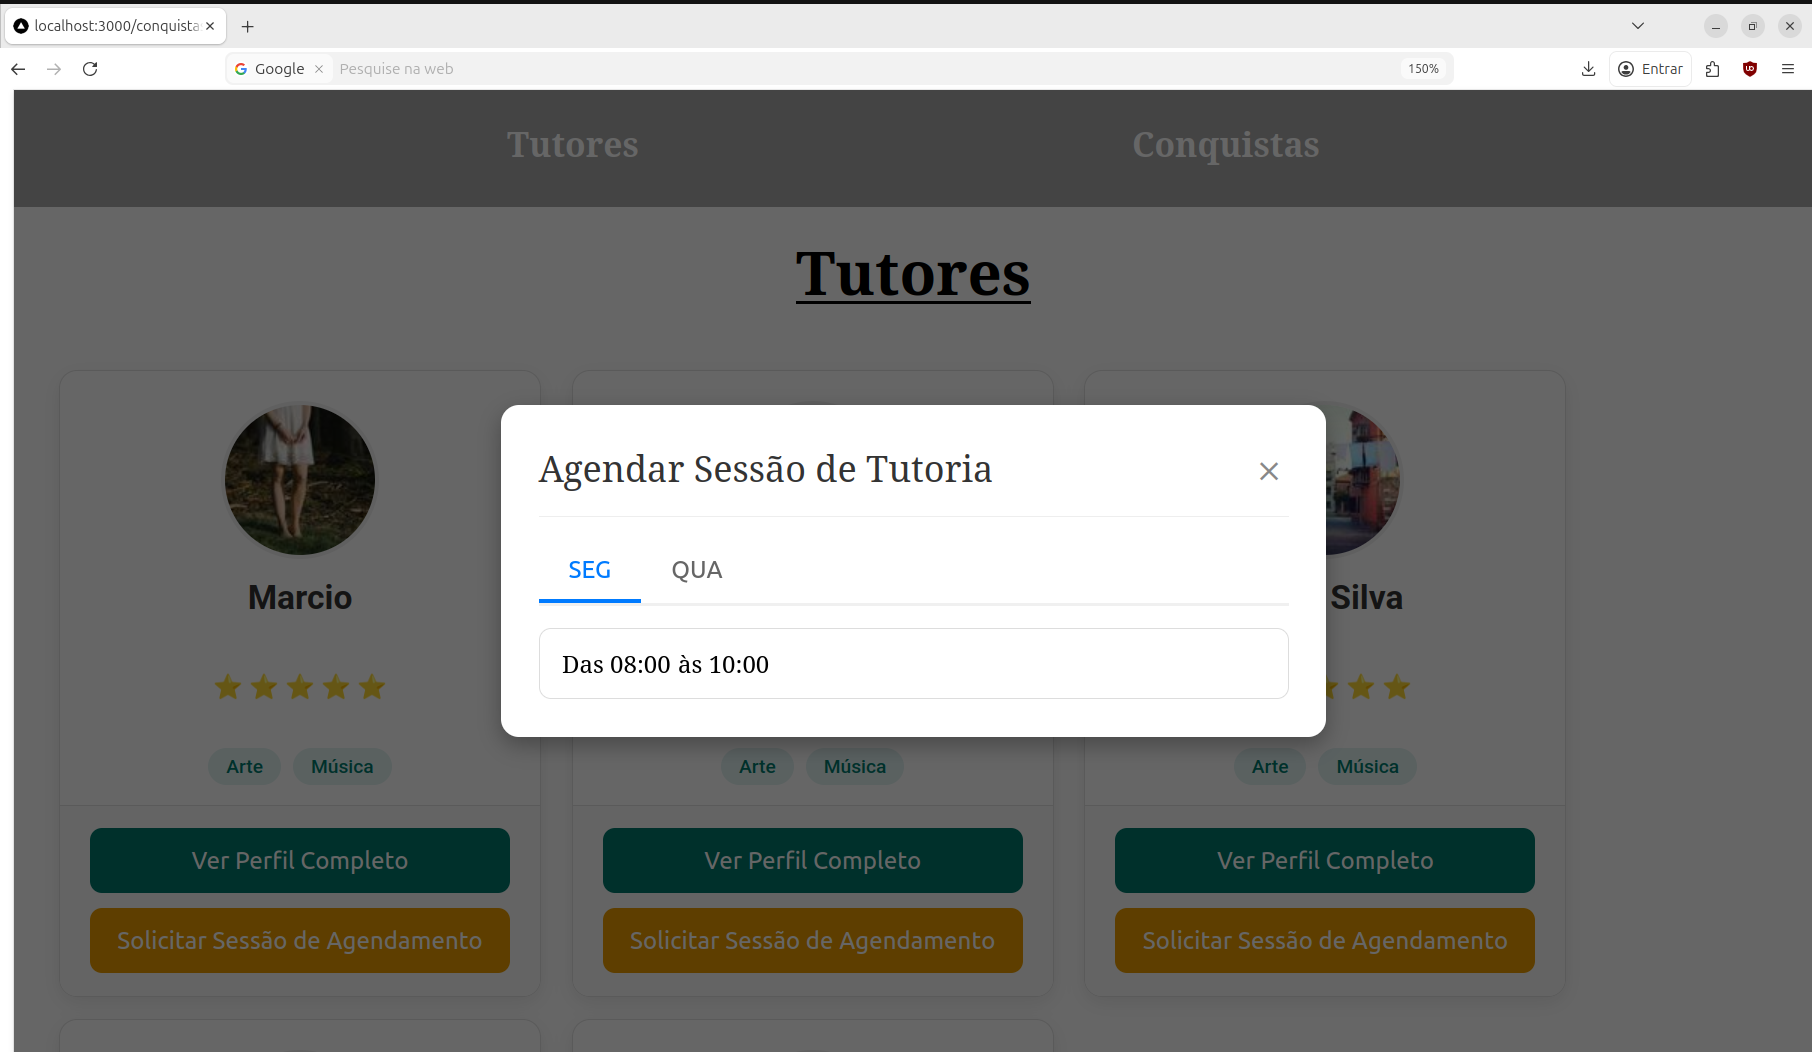
\includegraphics[width=0.99\textwidth]{figuras/sessao.png}


    Fonte: Autoria própria.
    
    \vspace{0.2cm}
        
    \label{fig:sessoes}
\end{figure}

Ao clicar em um horário, a solicitação de tutoria é realizada, a qual o tutor deve aceitar para que seja de fato confirmada. O usuário é notificado da realização da solicitação, conforme a Figura \ref{fig:notificacao-sessao}. Para melhor visualização, a janela de notificação pode ser vista isoladamente na Figura \ref{fig:notificacao-solitacao}. 

Como esta ação desbloqueia uma conquista, é exibida outra notificação, apresentada pela Figura \ref{fig:notificacao-conquista}. Para melhor visualização, a janela de notificação pode ser vista isoladamente na Figura \ref{fig:notificacao-conquista-isolada}. 

\newpage

\begin{figure}[h!]
    \centering

    \caption{Notificação de solicitação de tutoria.} 
    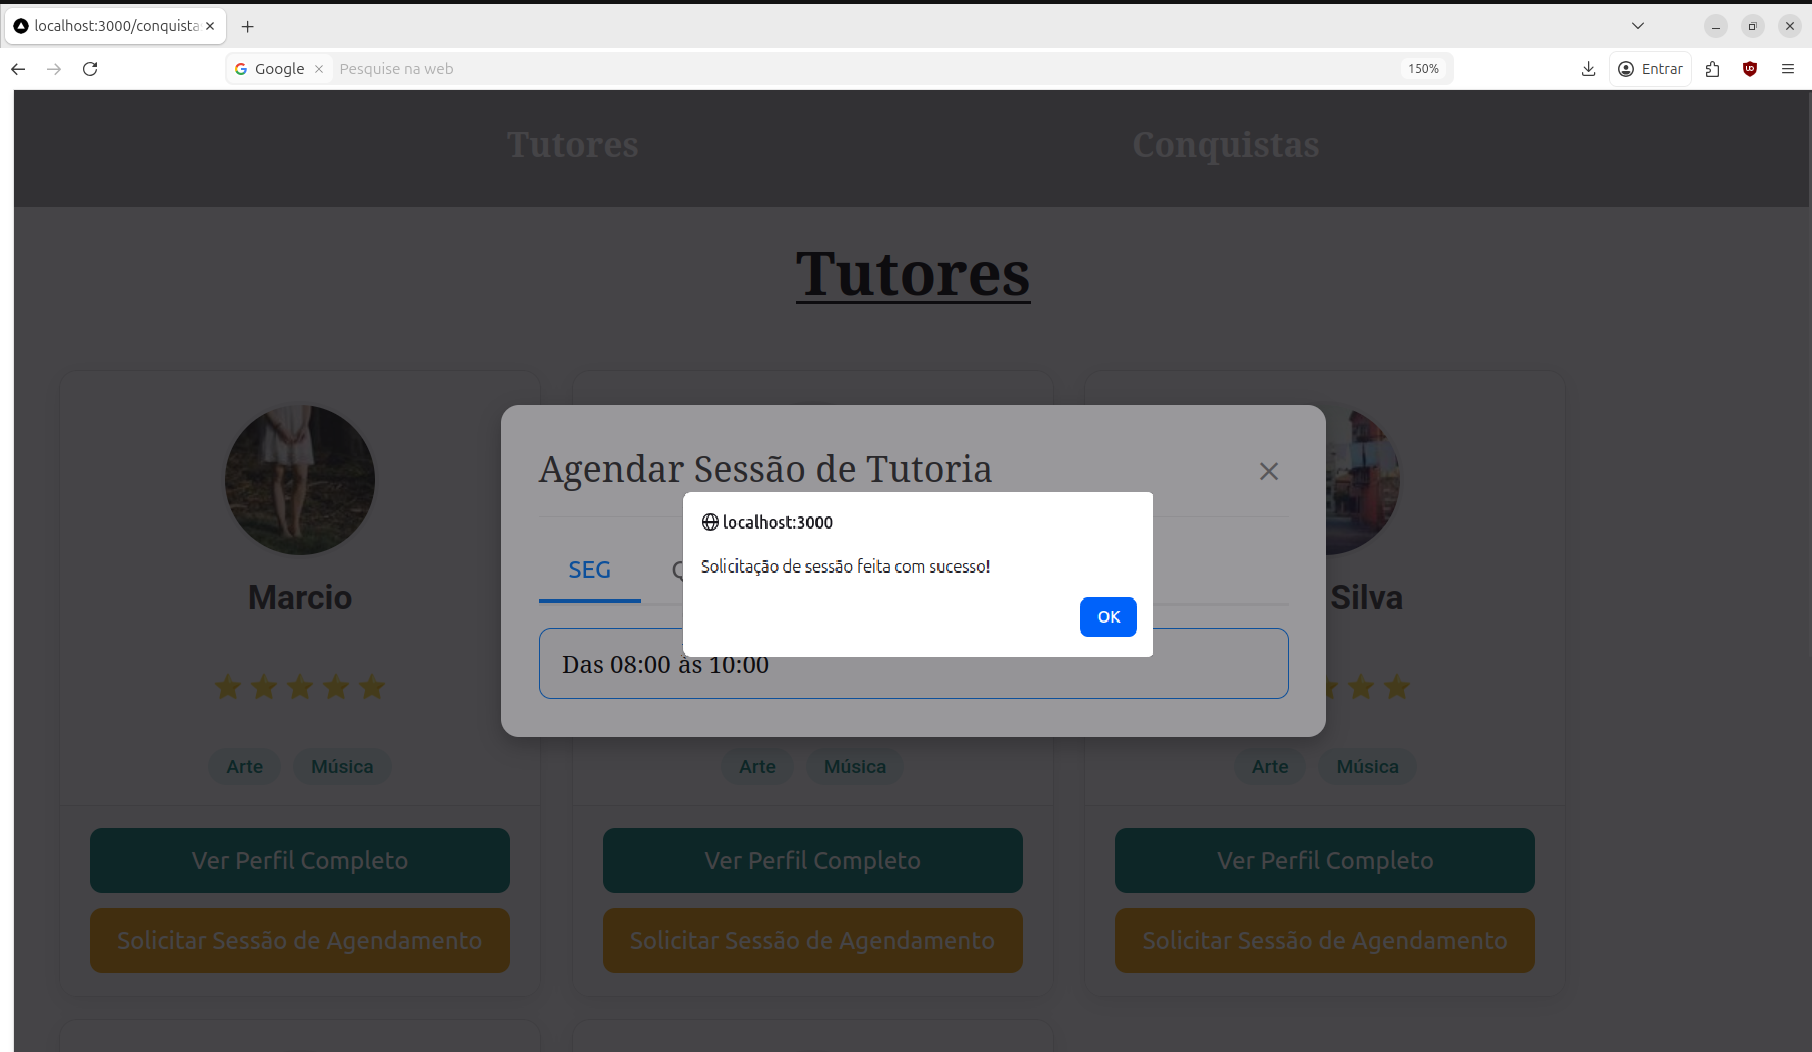
\includegraphics[width=0.99\textwidth]{figuras/notificacao-sessao.png}

    Fonte: Autoria própria.
    
    \vspace{0.2cm}
        
    \label{fig:notificacao-sessao}
\end{figure}

\begin{figure}[h!]
    \centering

    \caption{Janela de notificação de solicitação de tutoria.} 
    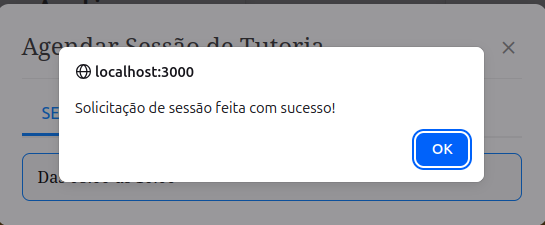
\includegraphics[width=0.75\textwidth]{figuras/notificacao-solitacao.png}

    Fonte: Autoria própria.
    
    \vspace{0.2cm}
        
    \label{fig:notificacao-solitacao}
\end{figure}

\newpage

\begin{figure}[h!]
    \centering

    \caption{Notificação de desbloqueio da conquista.} 
    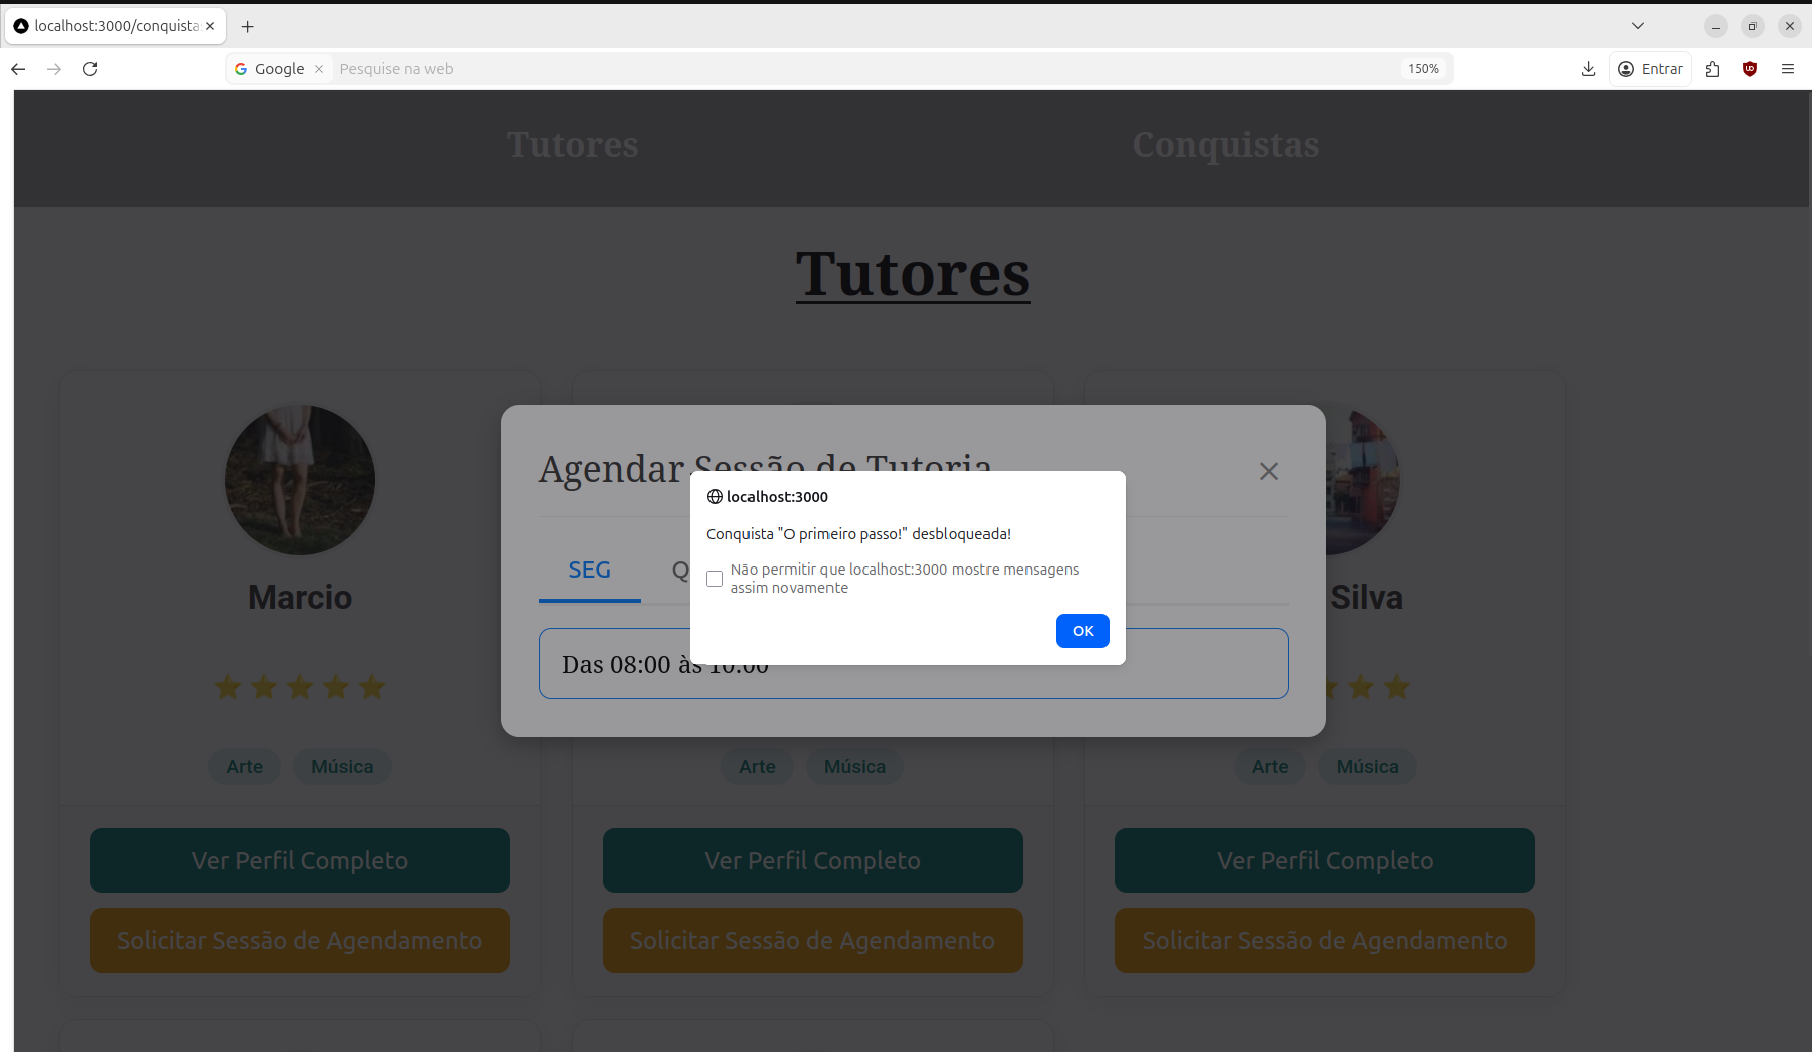
\includegraphics[width=0.99\textwidth]{figuras/notificacao-conquista.png}

    Fonte: Autoria própria.
    
    \vspace{0.2cm}
        
    \label{fig:notificacao-conquista}
\end{figure}

\begin{figure}[h!]
    \centering

    \caption{Janela de notificação de desbloqueio de conquistas.} 
    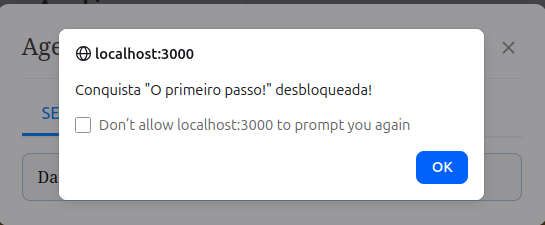
\includegraphics[width=0.75\textwidth]{figuras/notificacao-conquista-isolada.png}

    Fonte: Autoria própria.
    
    \vspace{0.2cm}
        
    \label{fig:notificacao-conquista-isolada}
\end{figure}

Ao voltar para a tela de conquistas, a conquista desbloqueada é apresentada em cores, conforme mostra a Figura \ref{fig:conquista-liberada}.

\newpage

\begin{figure}[h!]
    \centering
    \caption{Conquista desbloqueada.} 
    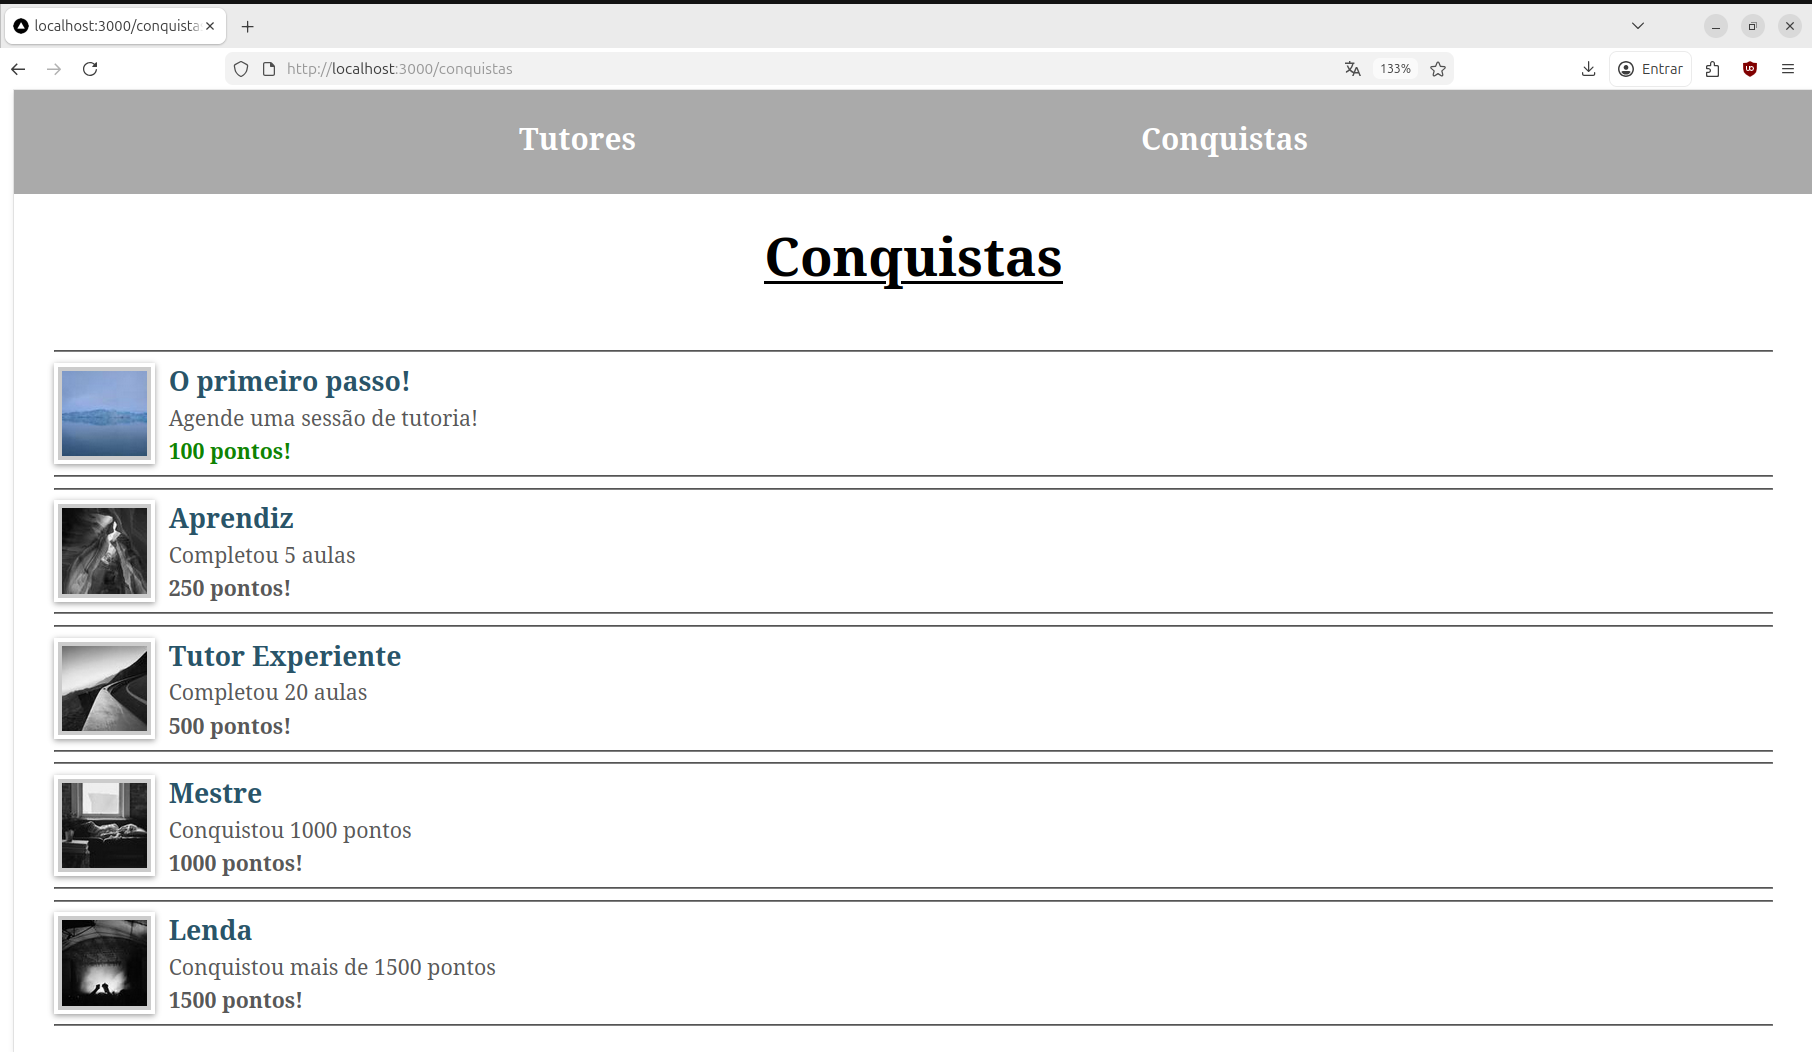
\includegraphics[width=0.99\textwidth]{figuras/conquista-liberada.png}


    Fonte: Autoria própria.
    
    \vspace{0.2cm}
        
    \label{fig:conquista-liberada}
\end{figure}

A simulação tornou possível perceber que a arquitetura proposta consegue realizar a integração entre o \textit{backend} e o \textit{frontend} de forma satisfatória, além de demonstrar a capacidade de realizar consultas e registros na base de dados modelada. Assim, a arquitetura atende as
necessidades da proposta e é viável para o desenvolvimento do projeto.


\chapter[\textit{Lean Inception}]{\textit{Lean Inception}}
\label{lean-inception}

O \textit{Lean Inception} foi desenvolvido no Figma, adaptado a partir do template disponível em \href{caroli.org}{caroli.org}, podendo ser acessado pelo \href{https://www.figma.com/board/xXIvddv95LAyy0uTLGtEIc/TCC-Vandor?node-id=0-1&t=AienmrKhFTuCnwu8-1}{link}.

\begin{figure}[h!]
    \centering
    \caption{Visão do Produto.} 
    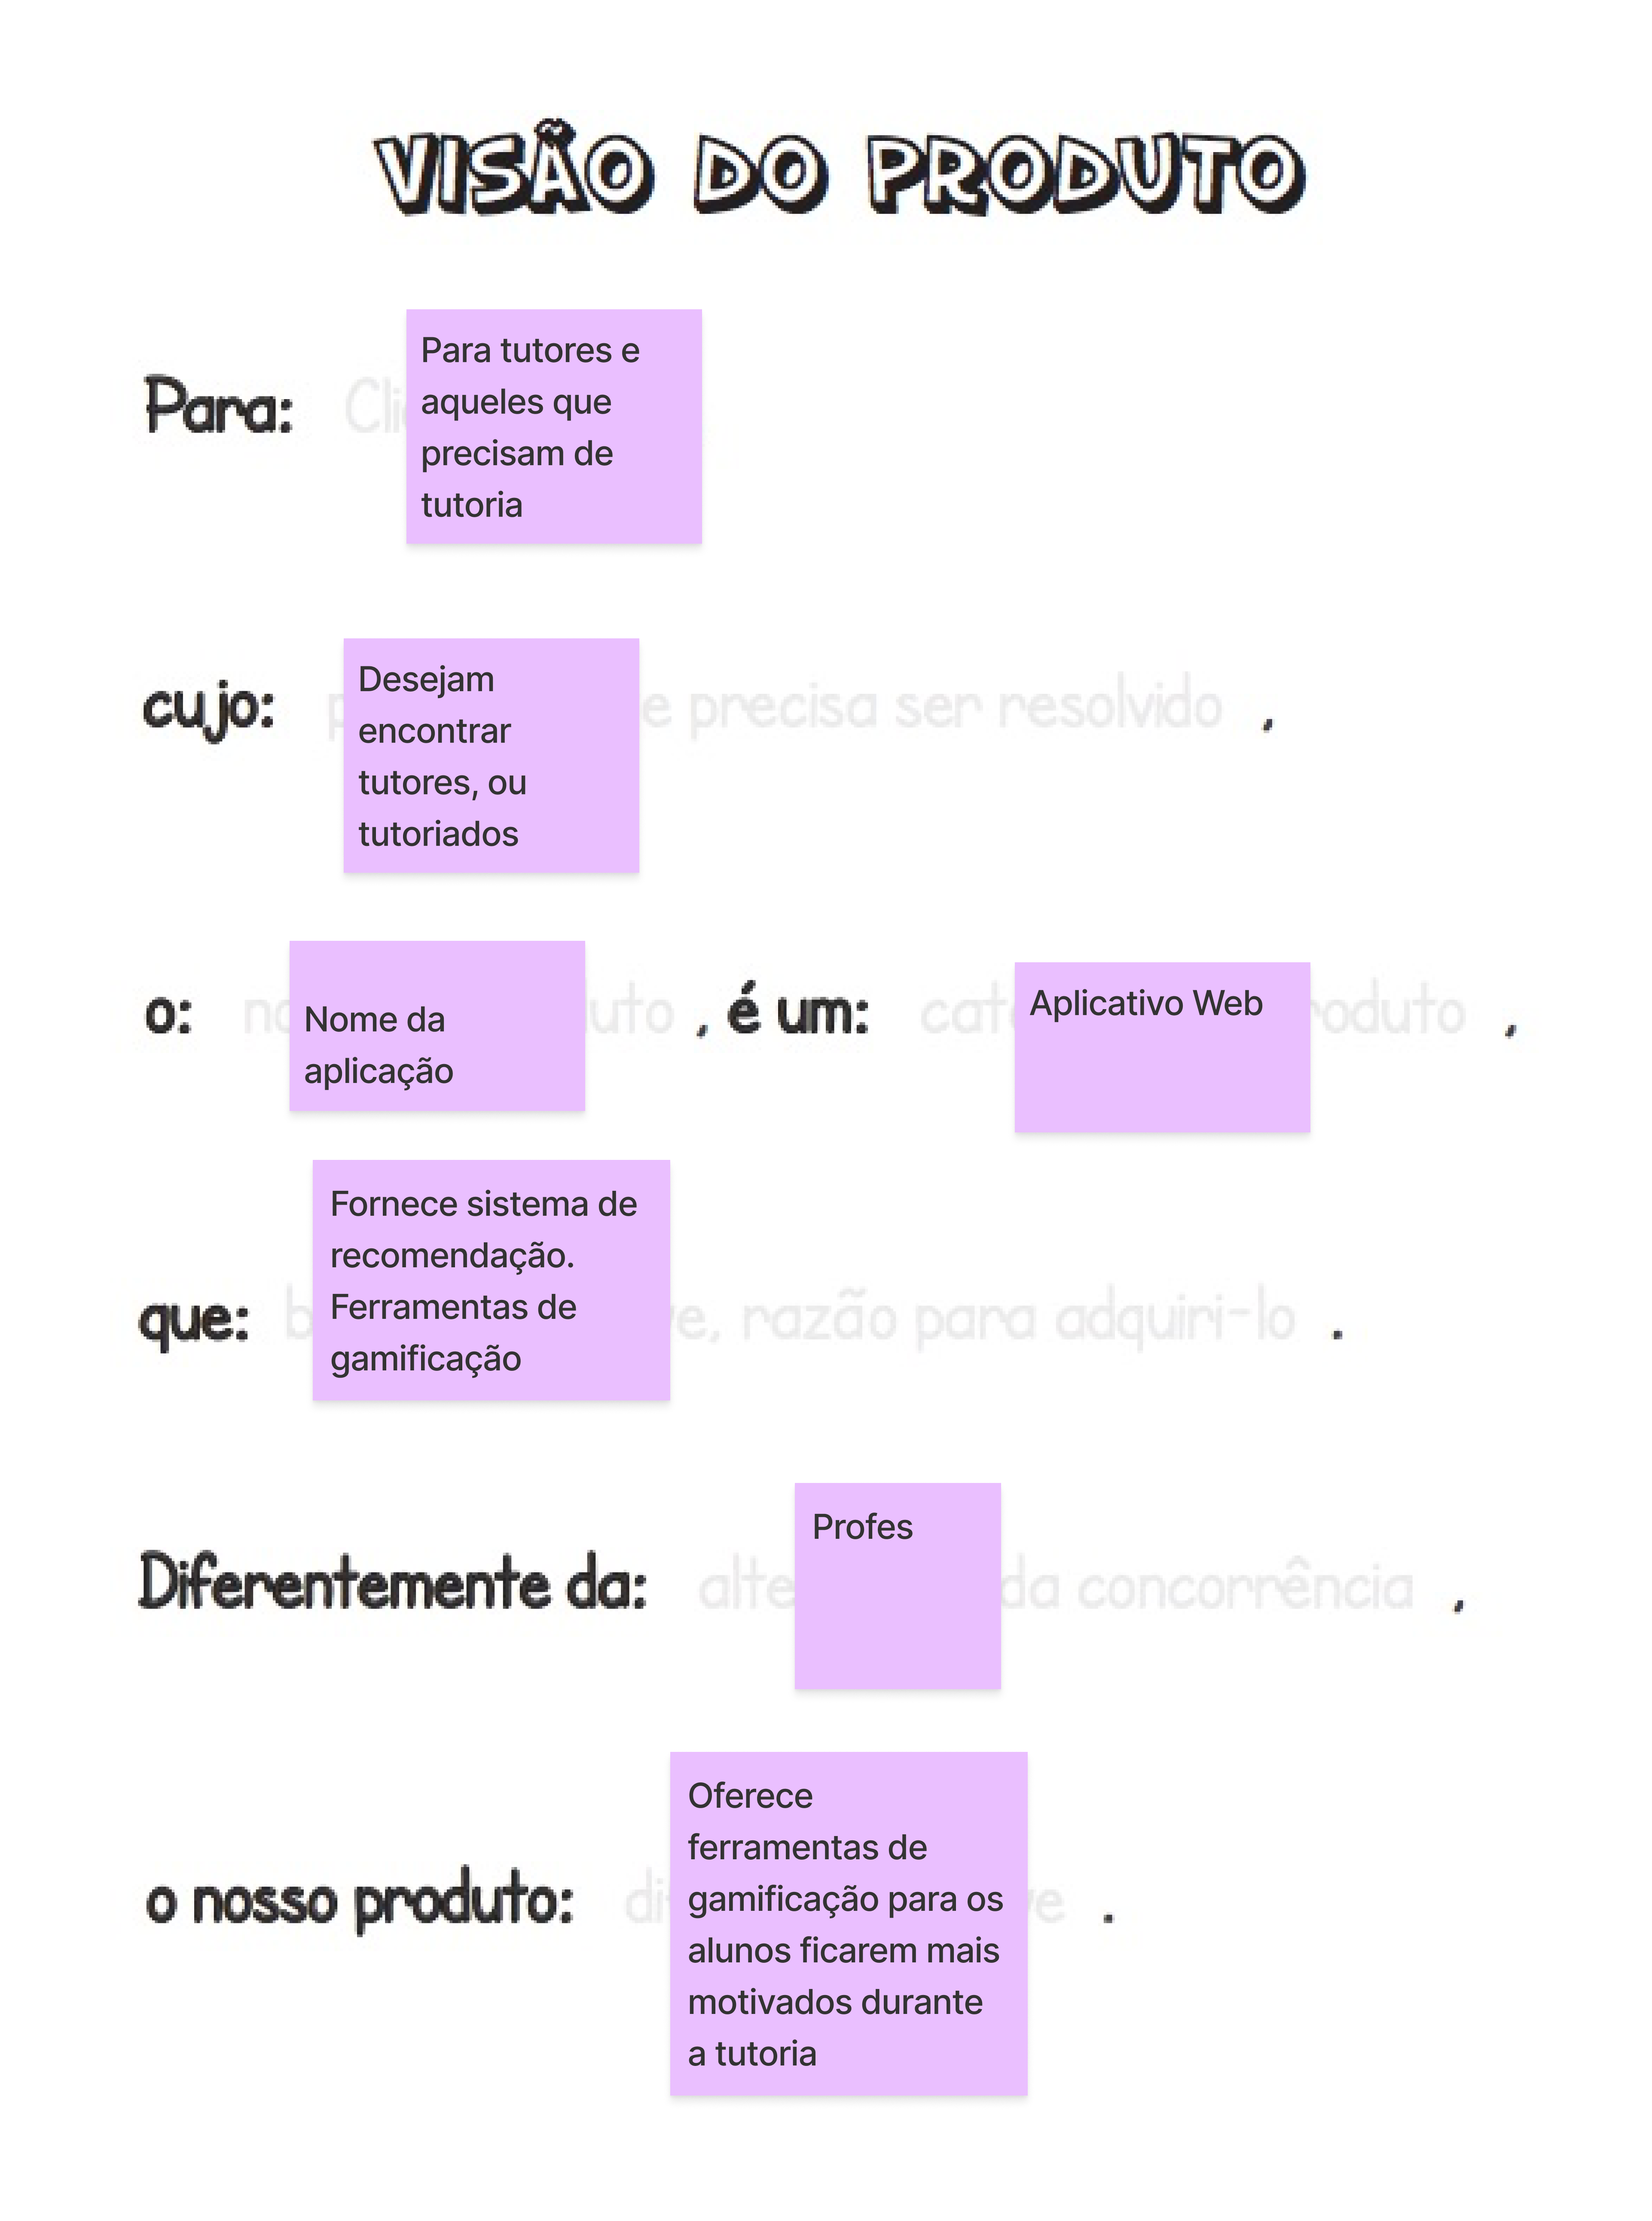
\includegraphics[width=0.9\textwidth]{figuras/Lean01VisaoProduto.png}

    Fonte: Adaptado a partir de caroli.org
    
    \vspace{0.2cm}
\end{figure}

\begin{figure}[h!]
    \centering
    \caption{Seção do que o software é.} 
    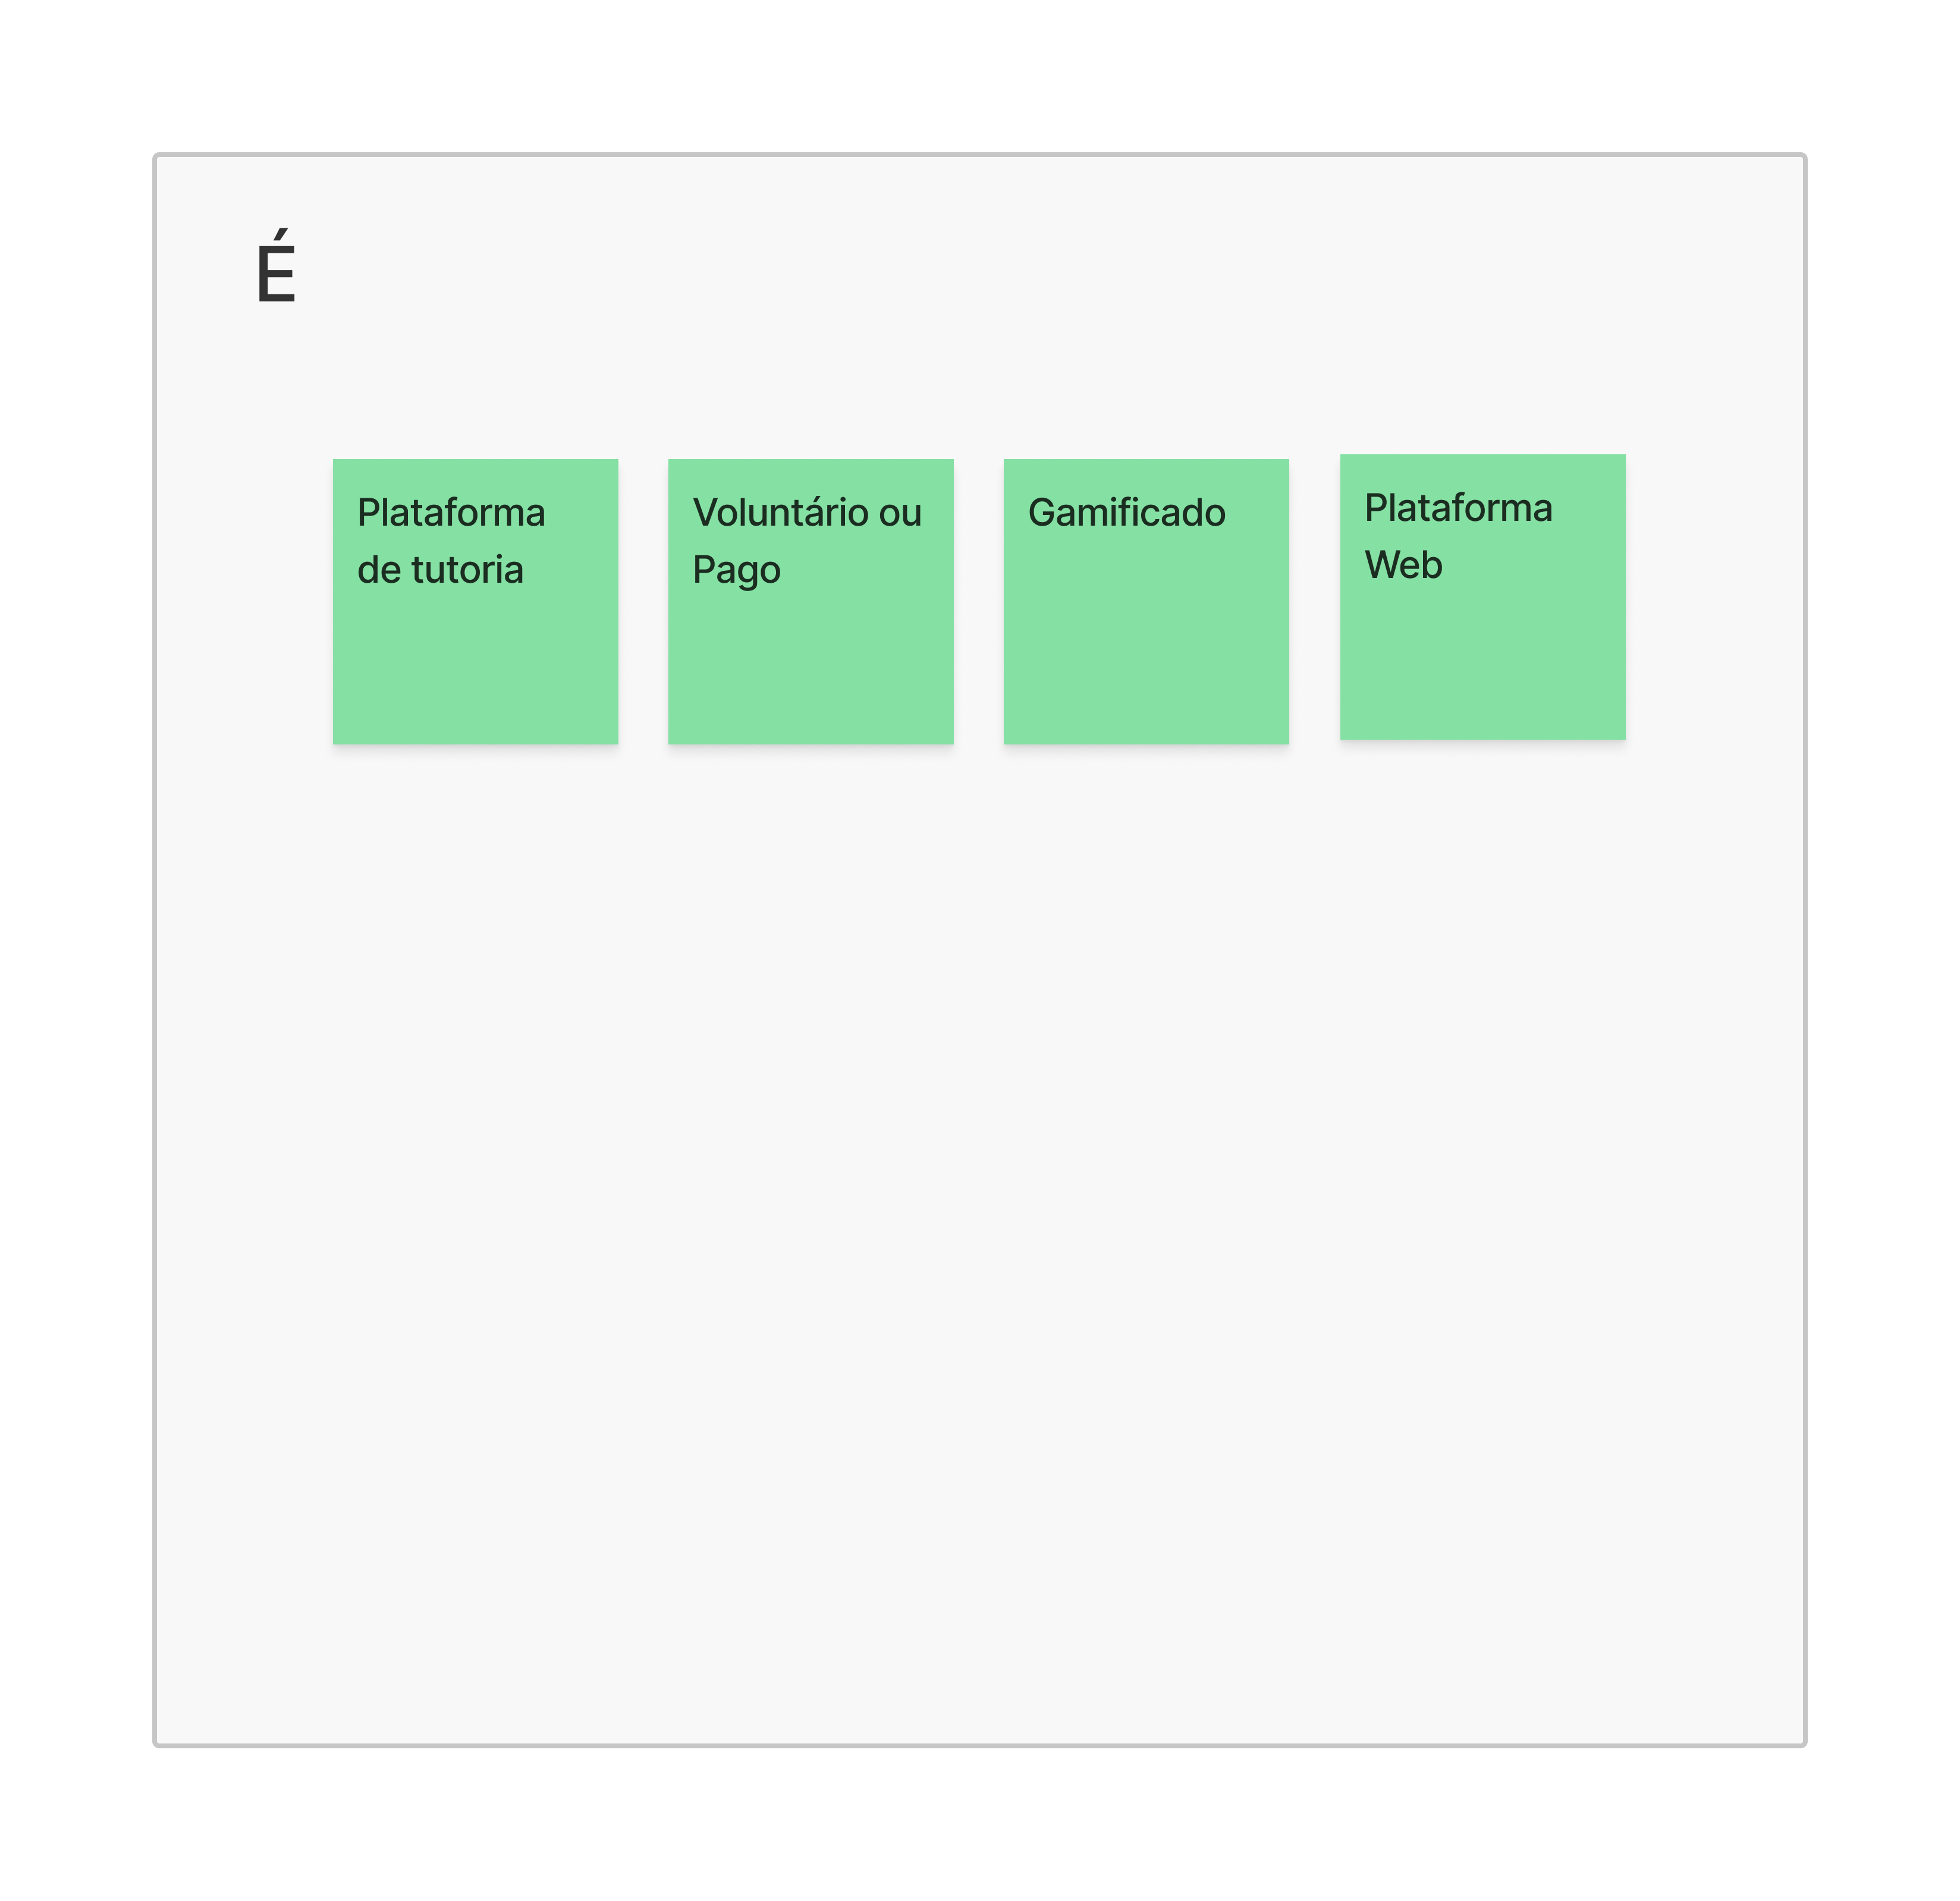
\includegraphics[width=0.9\textwidth]{figuras/Lean02Eh.png}
       
    Fonte: Adaptado a partir de caroli.org
    
    \vspace{0.2cm}
\end{figure}

\begin{figure}[h!]
    \centering
    \caption{Seção do que o software não é.} 
    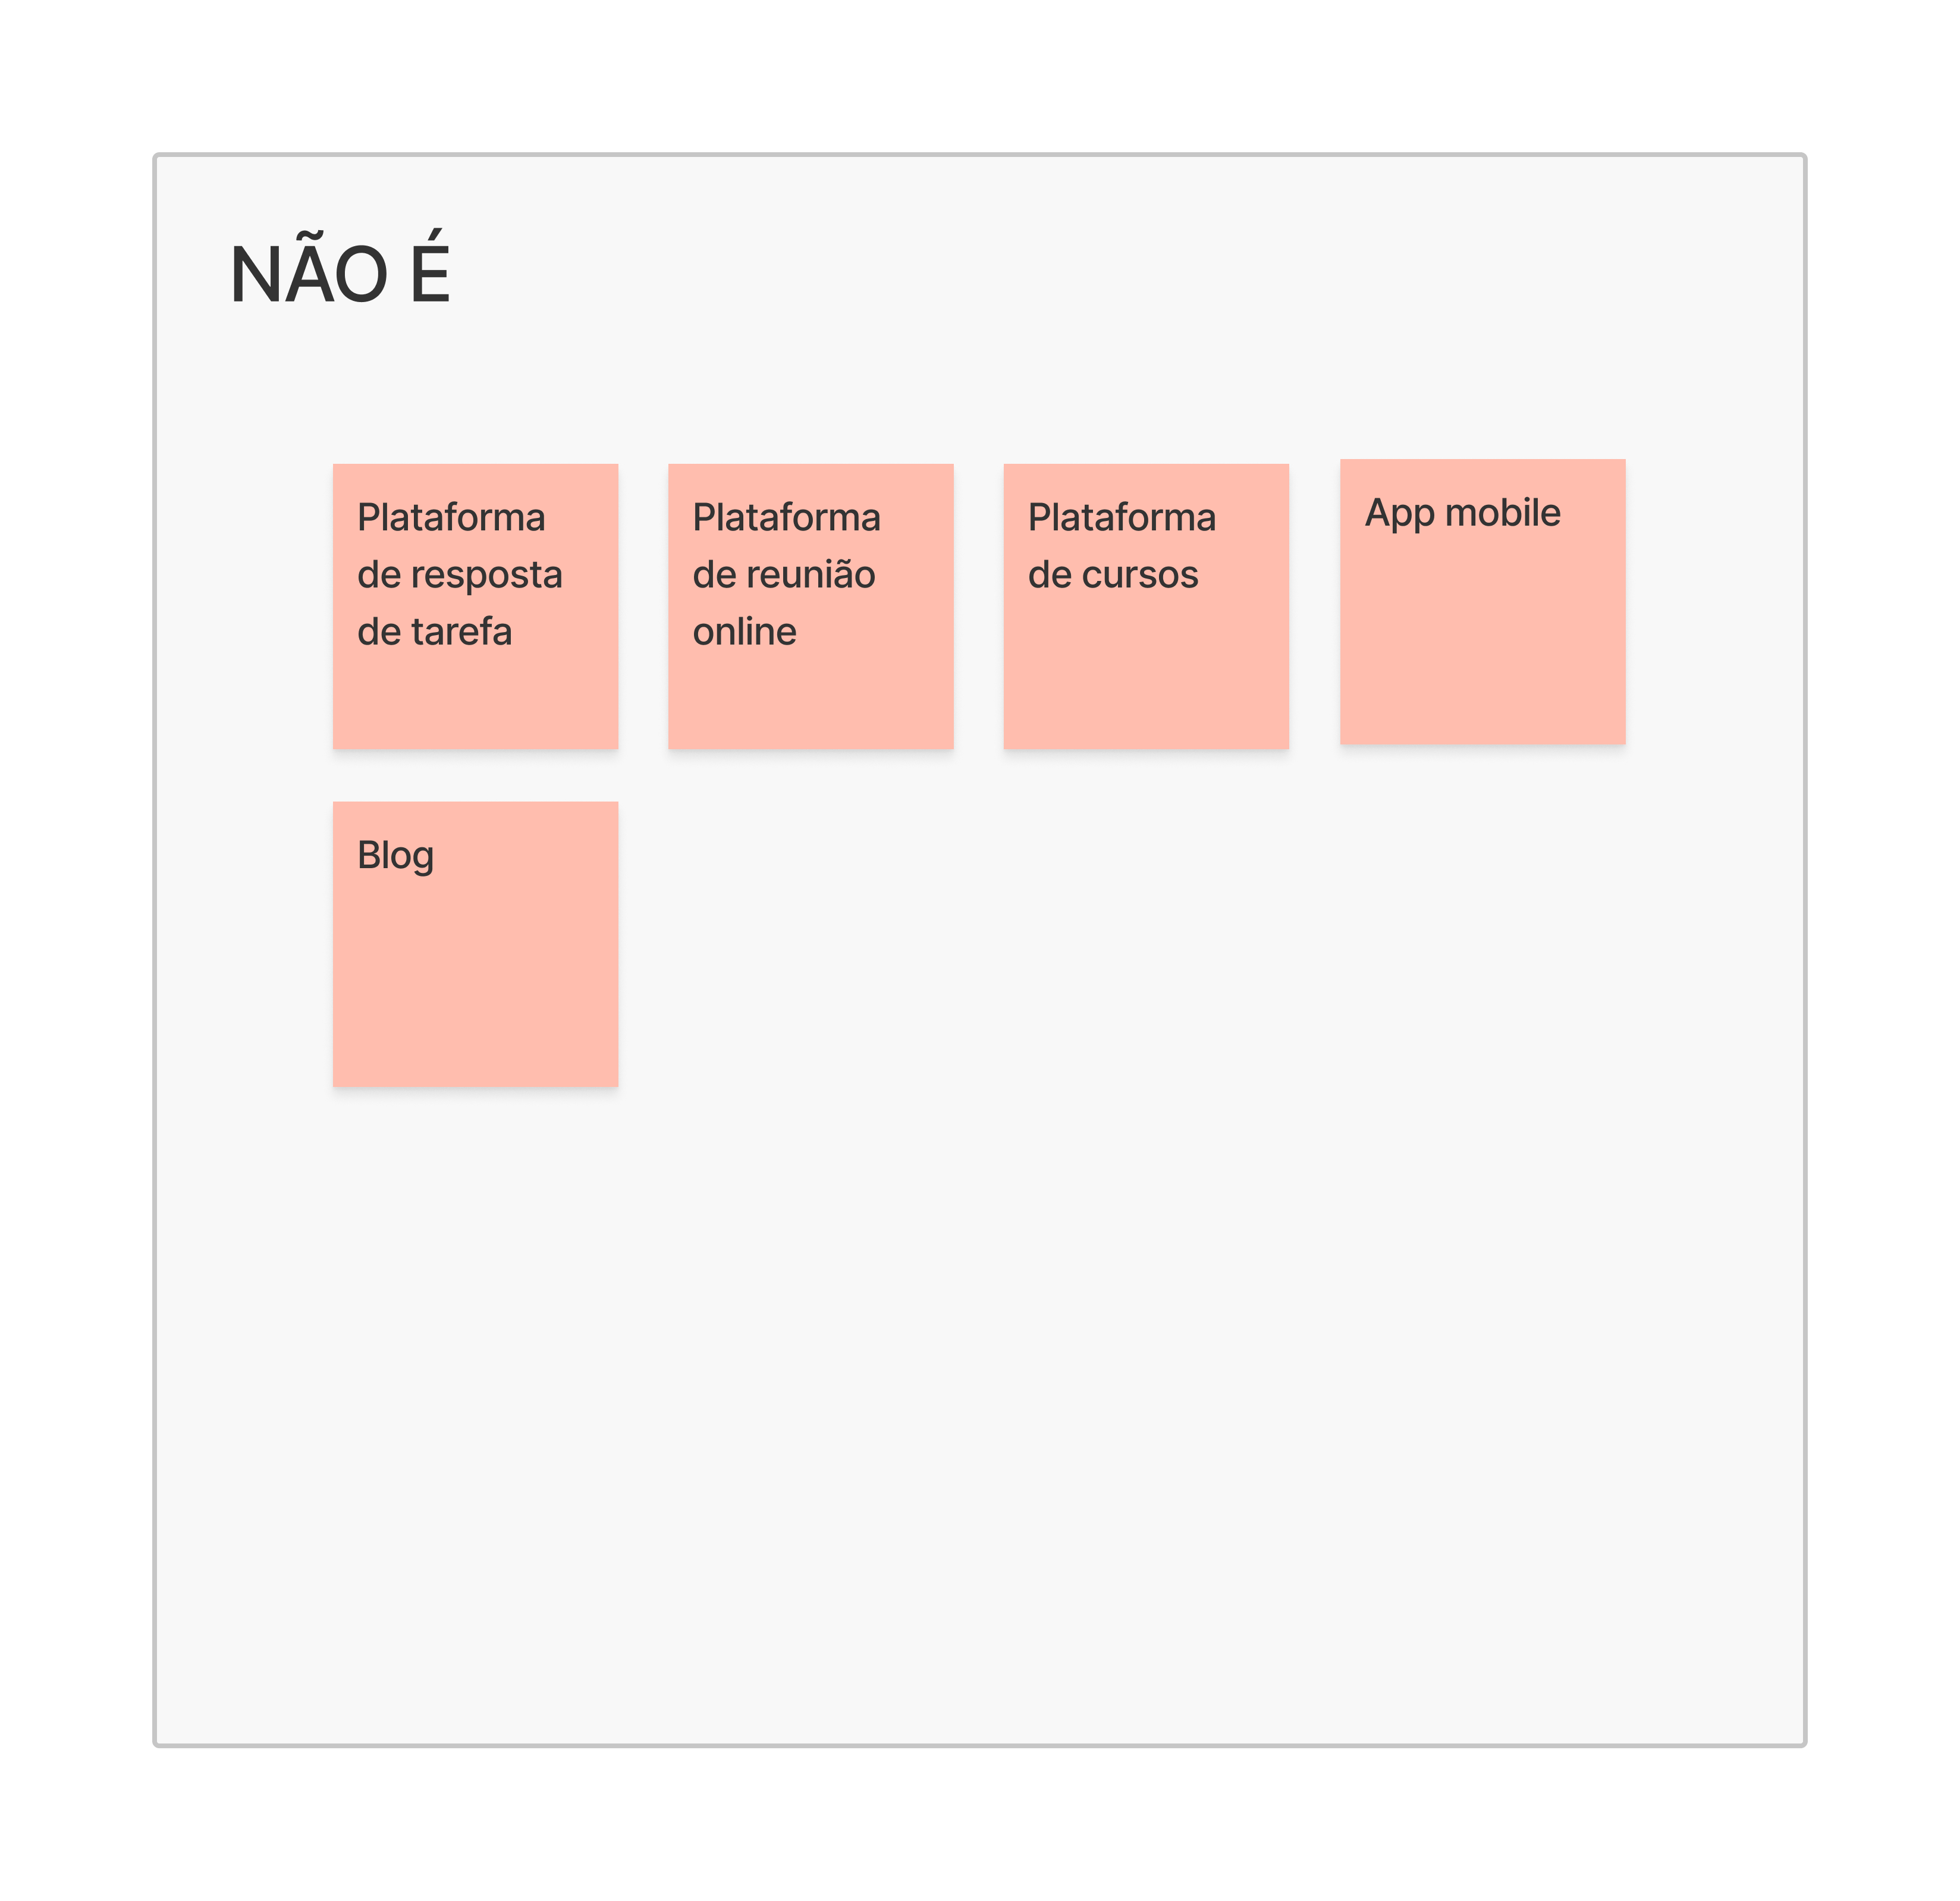
\includegraphics[width=0.9\textwidth]{figuras/Lean02NaoEh.png}

    Fonte: Adaptado a partir de caroli.org

    
    \vspace{0.2cm}
\end{figure}

\begin{figure}[h!]
    \centering
    \caption{Seção do que o software faz.} 
    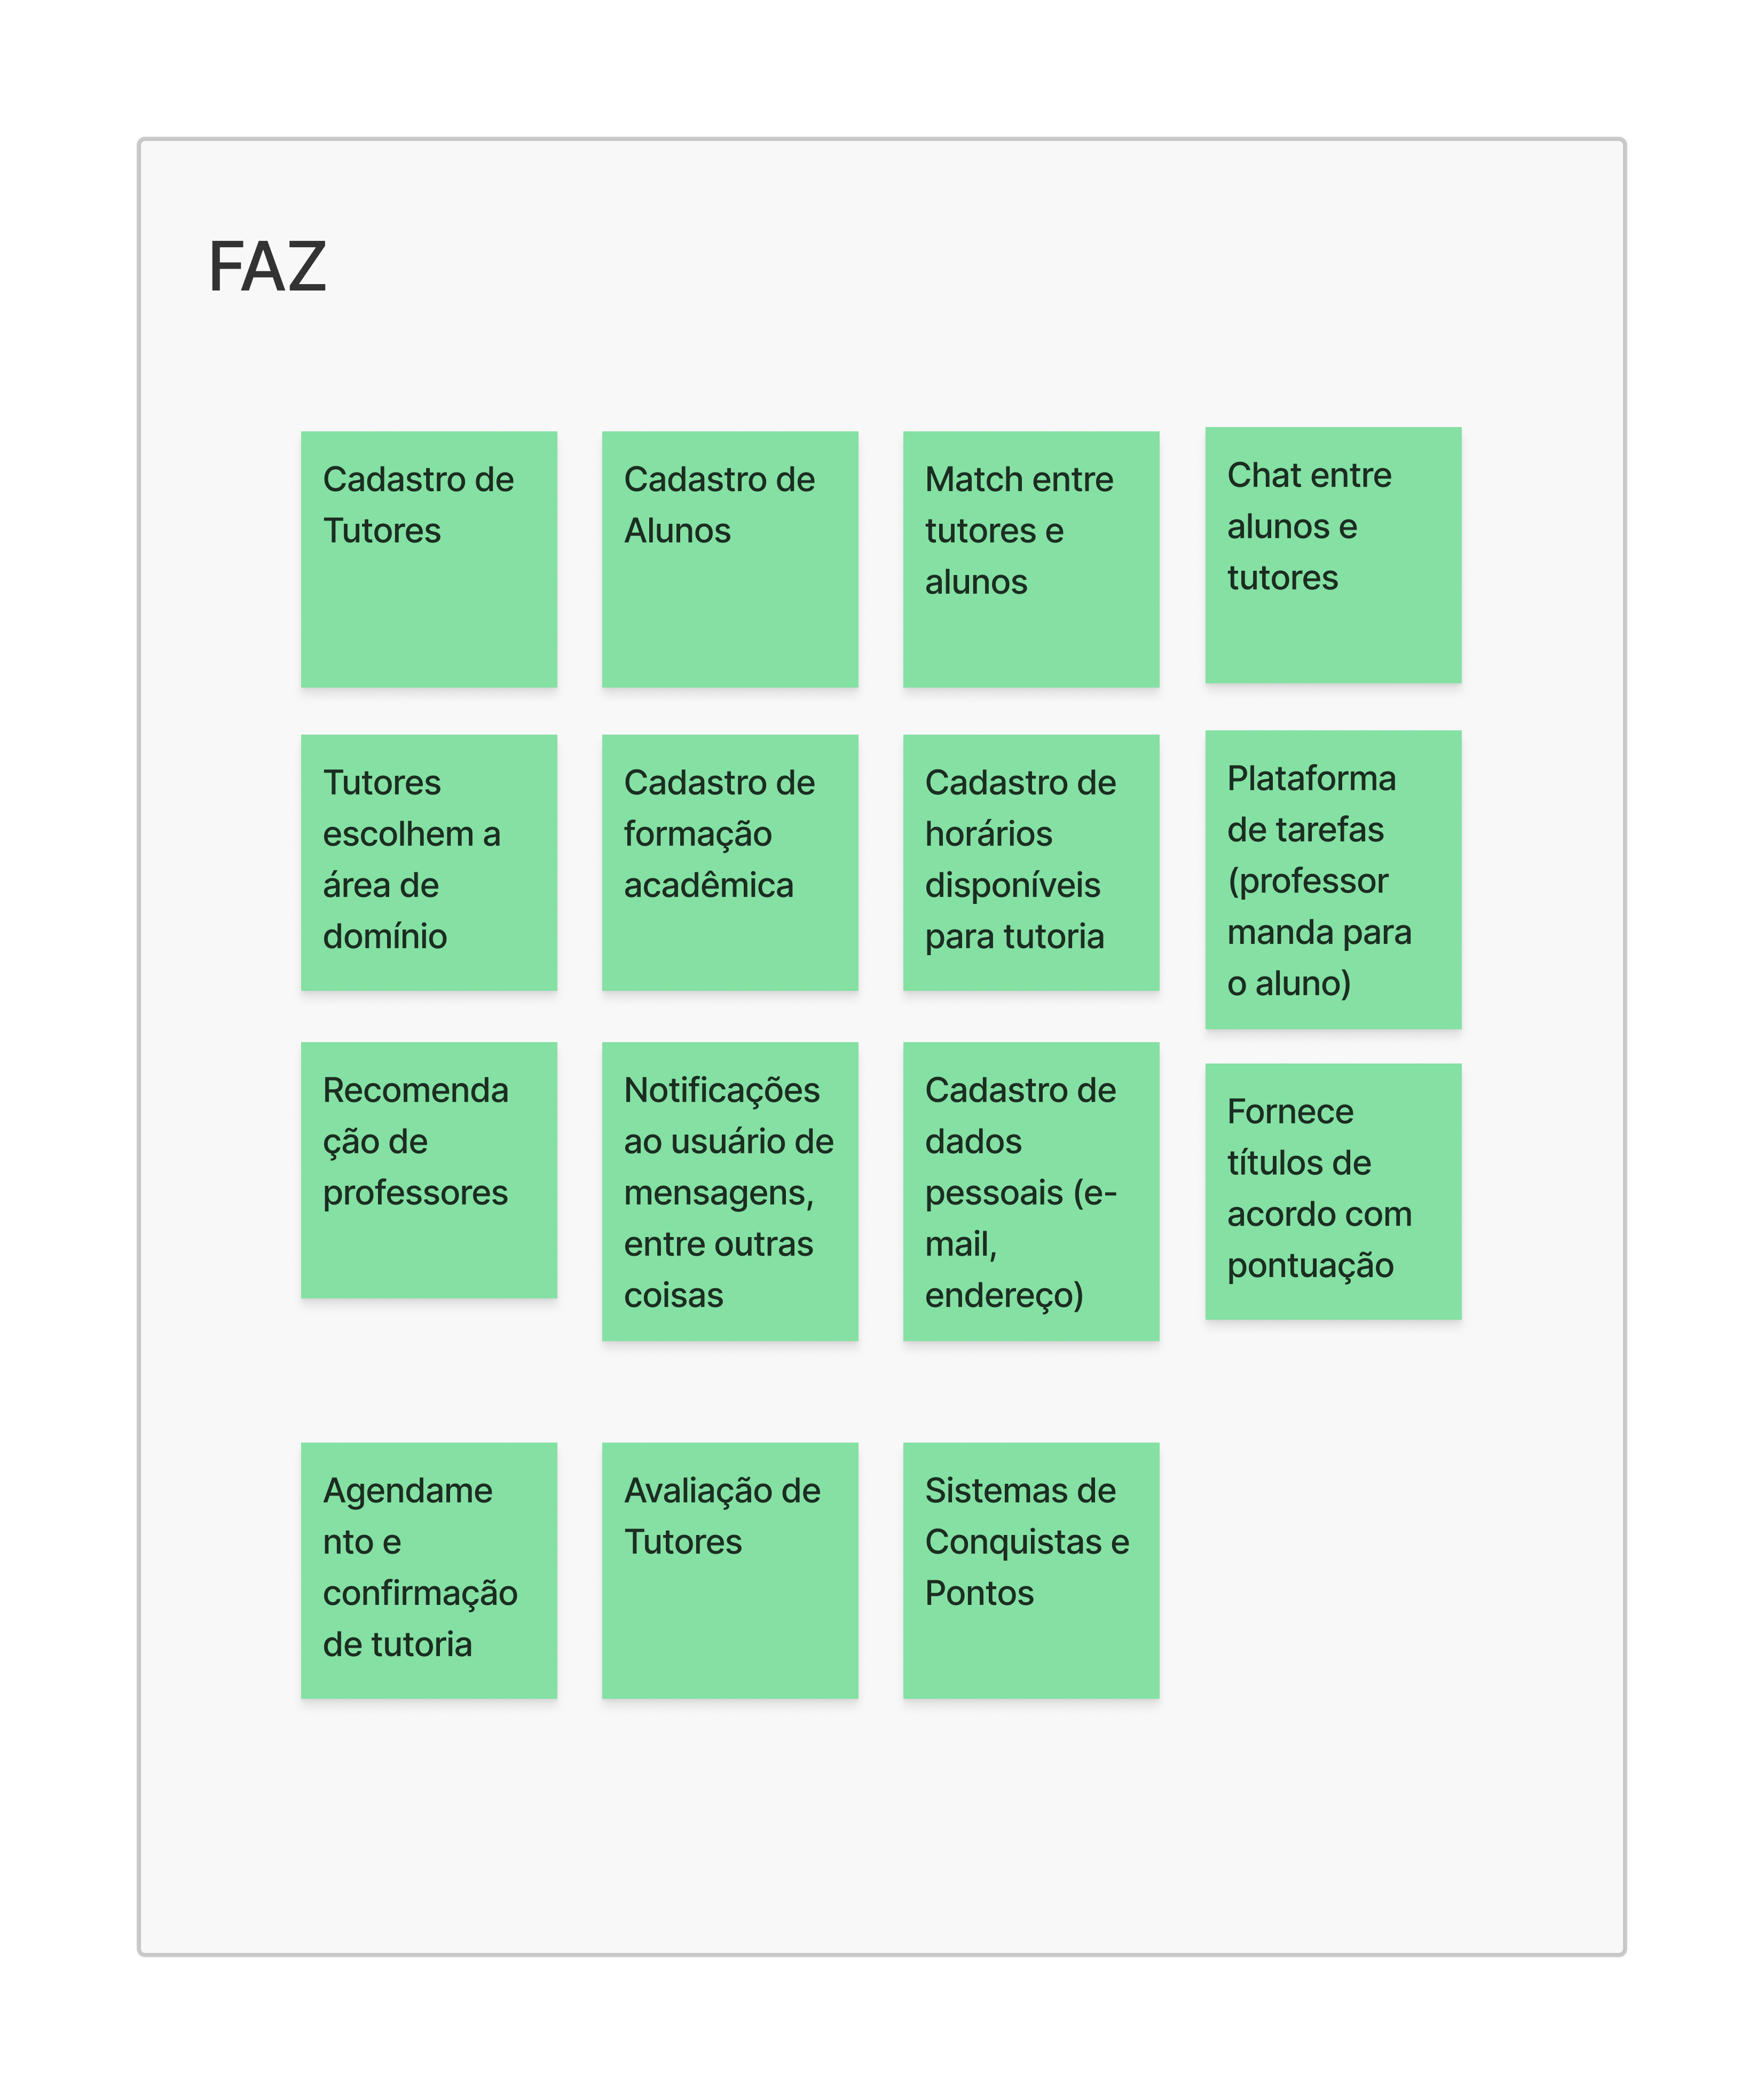
\includegraphics[width=0.9\textwidth]{figuras/Lean02Faz.png}

    Fonte: Adaptado a partir de caroli.org
    
    \vspace{0.2cm}
\end{figure}

\begin{figure}[h!]
    \centering
    \caption{Seção do que o software não faz.} 
    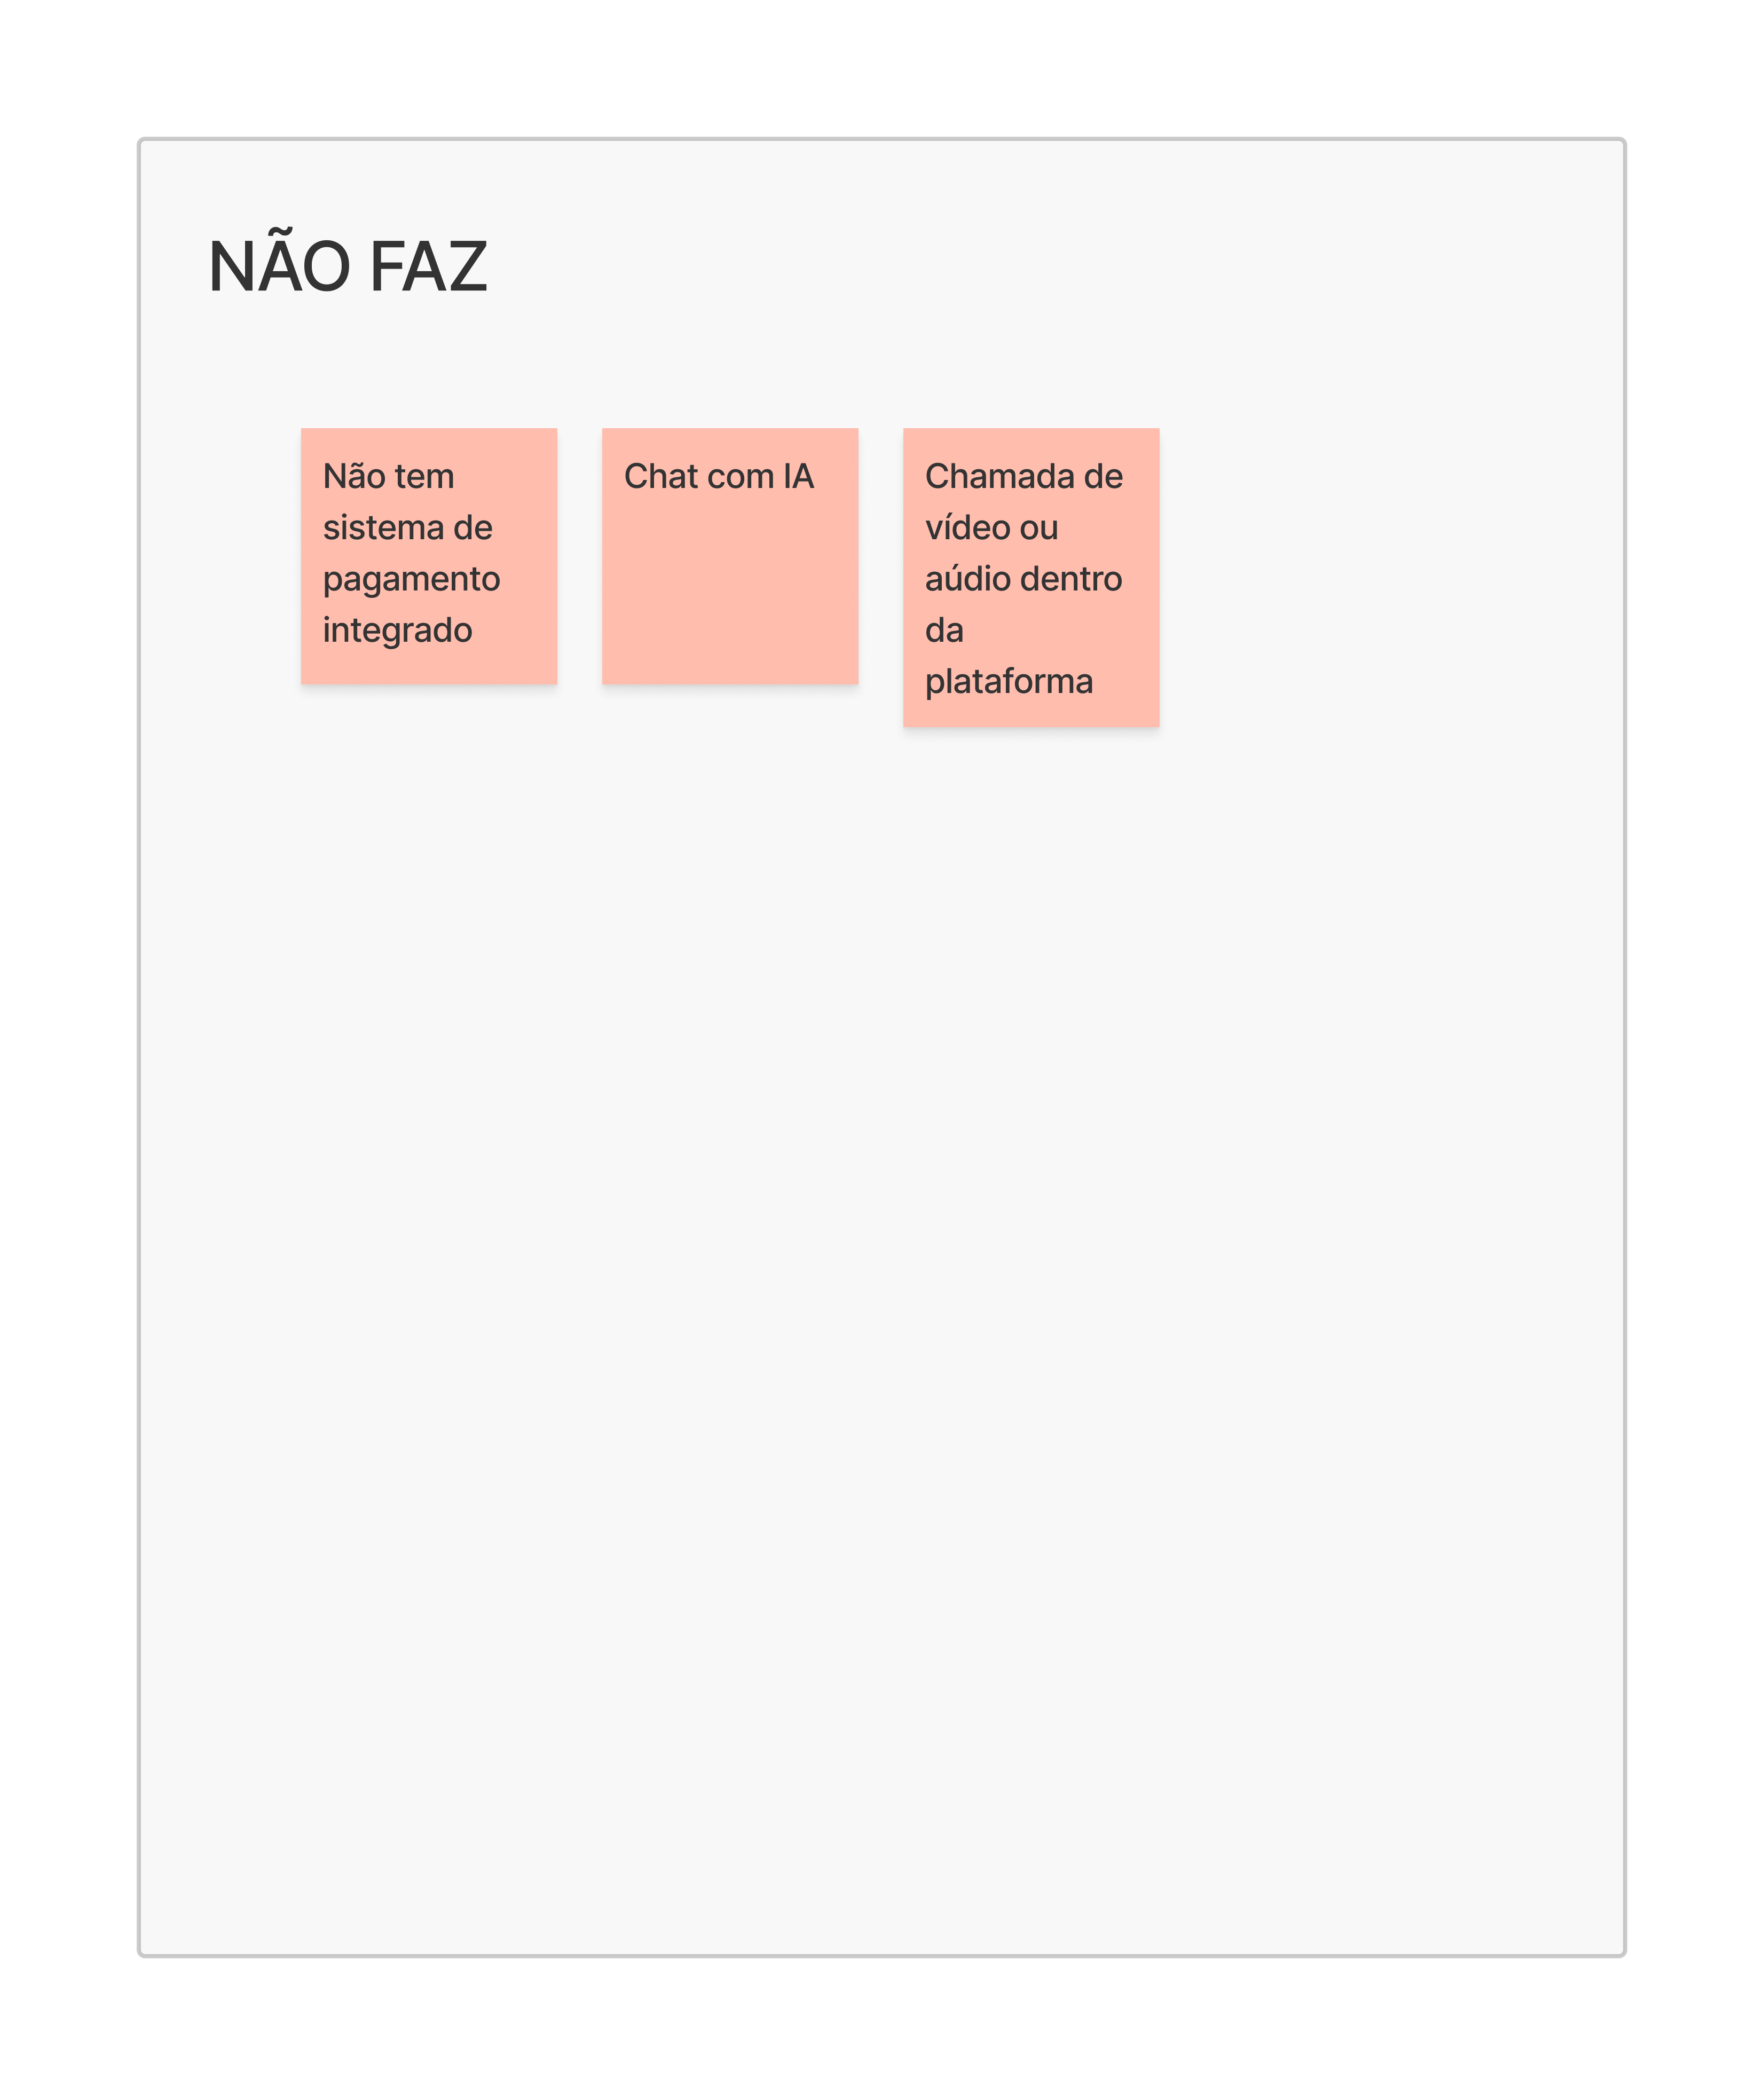
\includegraphics[width=0.9\textwidth]{figuras/Lean02NaoFaz.png}

    Fonte: Adaptado a partir de caroli.org

    \vspace{0.2cm}
\end{figure}

\begin{figure}[h!]
    \centering
    \caption{Objetivos do Produto.} 
    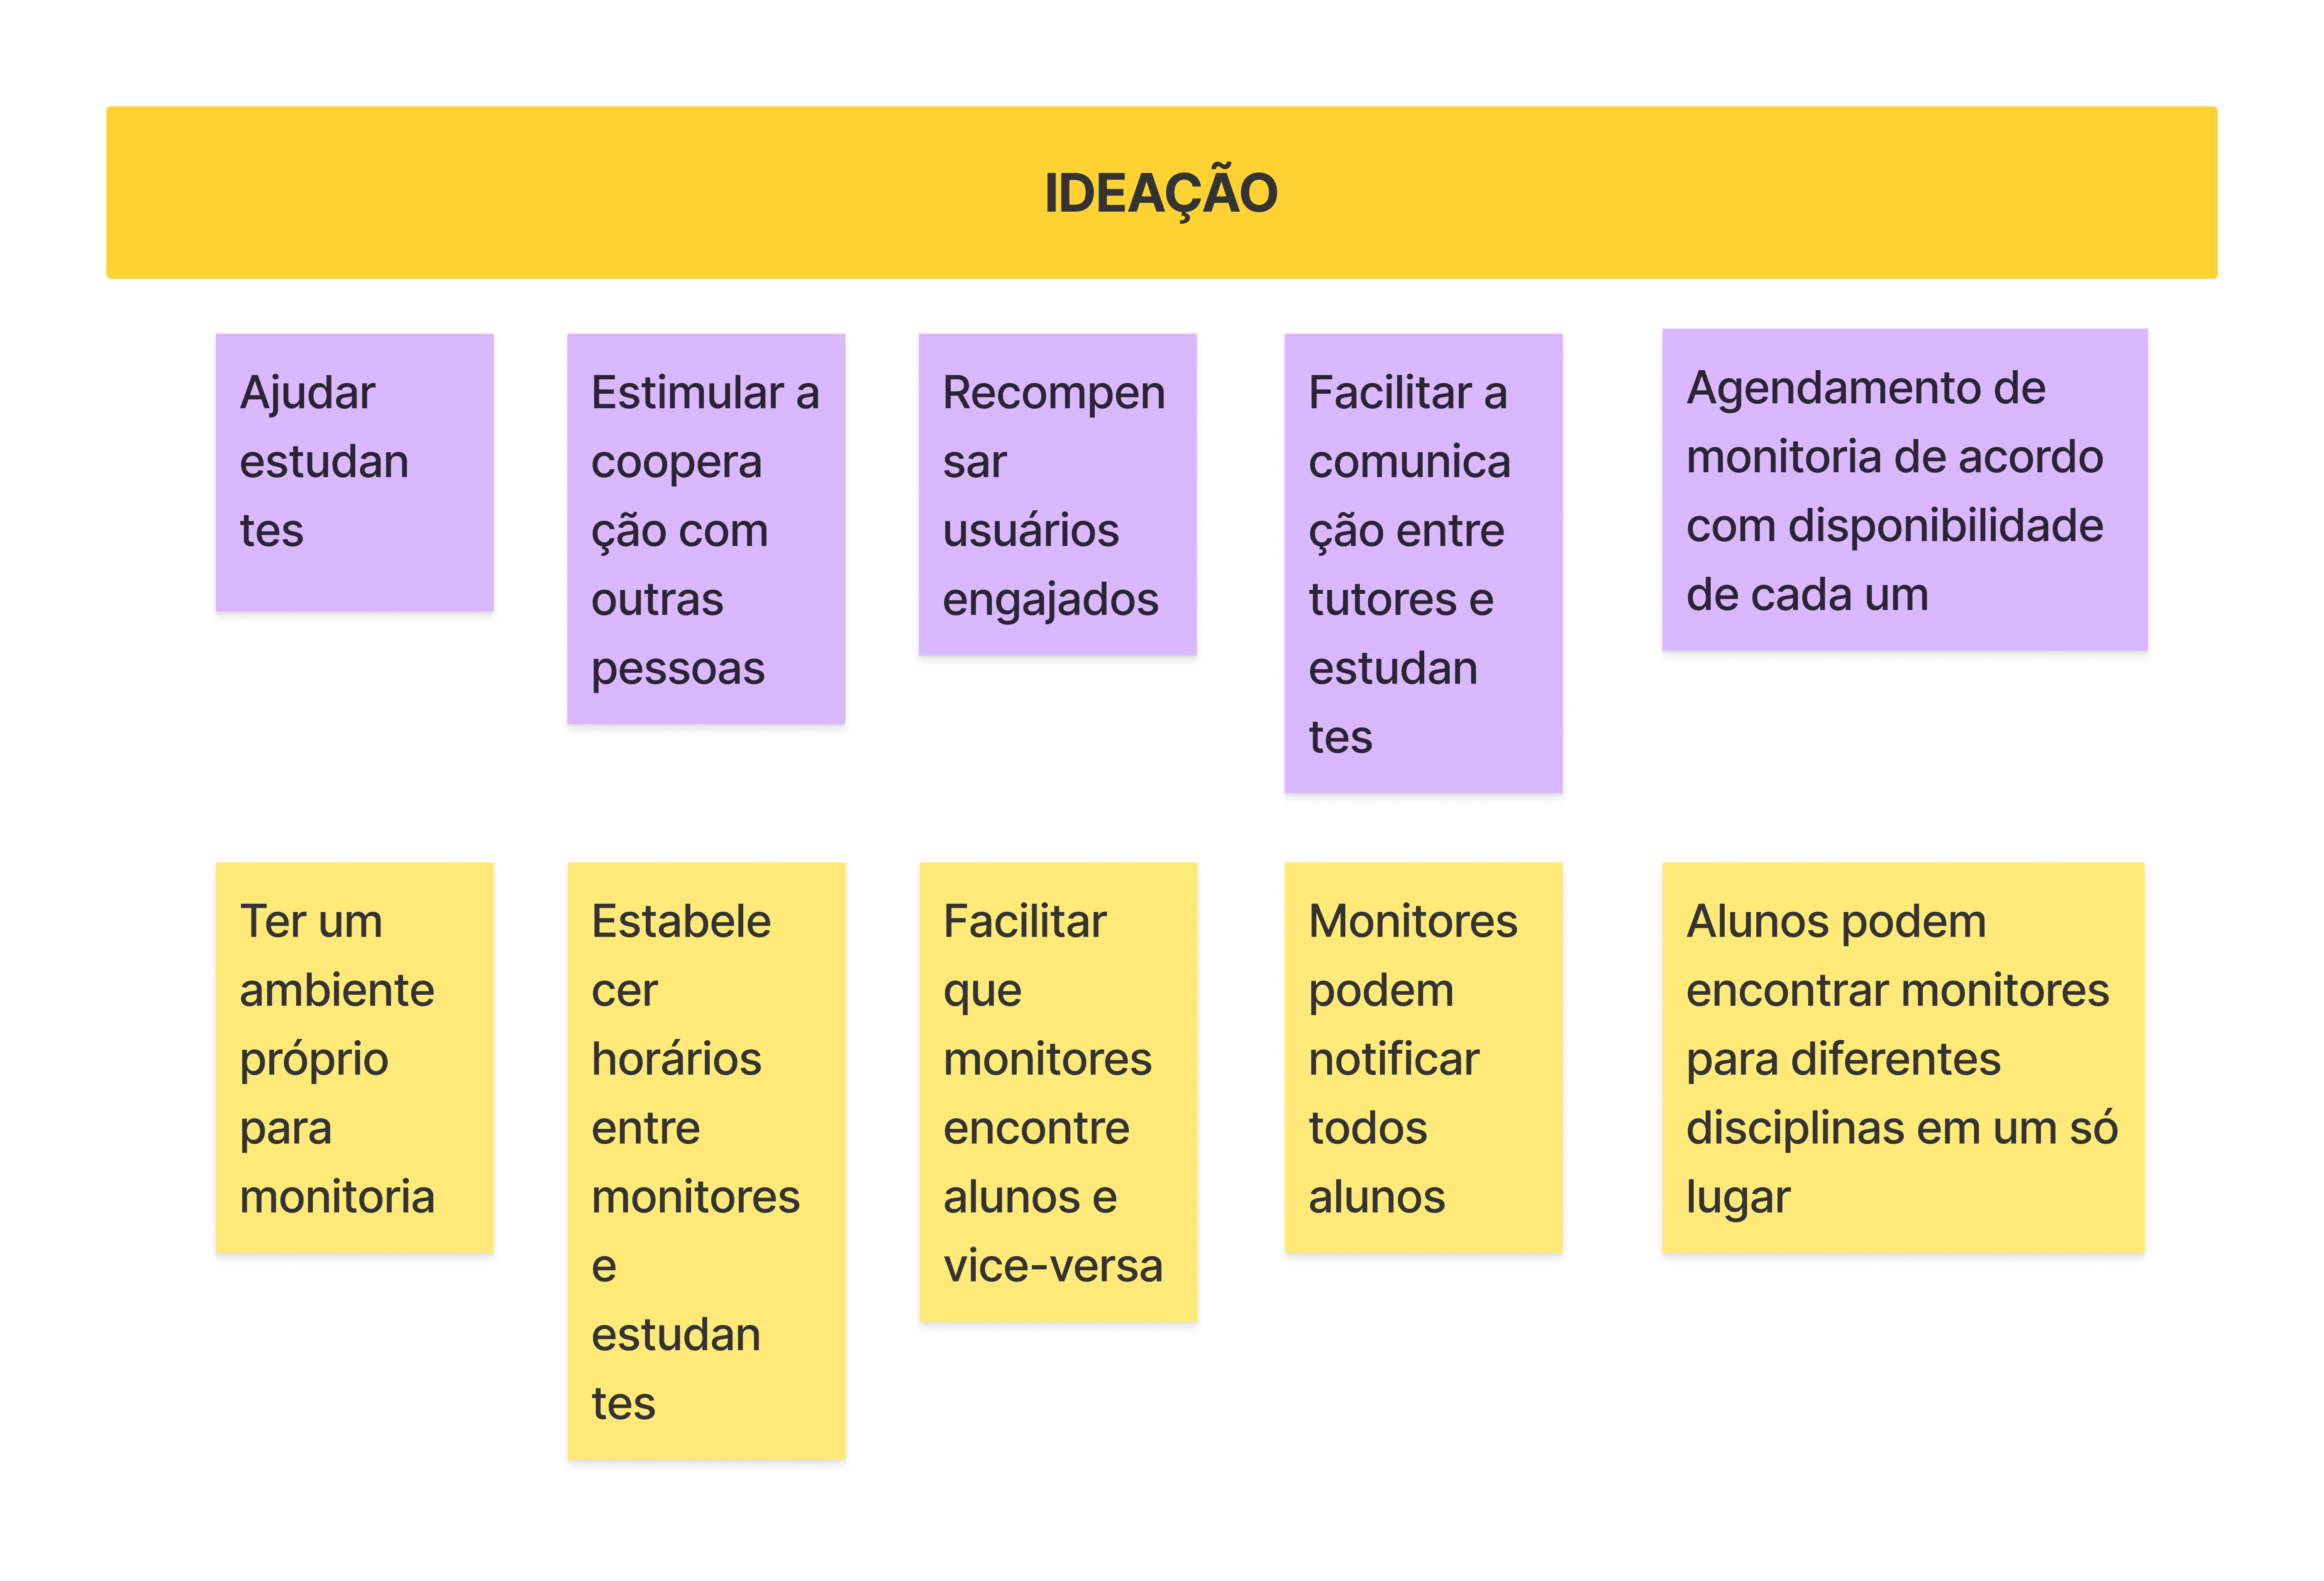
\includegraphics[width=0.9\textwidth]{figuras/Lean03Ideacao.png}

    Fonte: Adaptado a partir de caroli.org
    
    \vspace{0.2cm}
\end{figure}

\begin{figure}[h!]
    \centering
    \caption{Ideias de funcionalidades (Gamificação, Comunicação, Recomendação).} 
    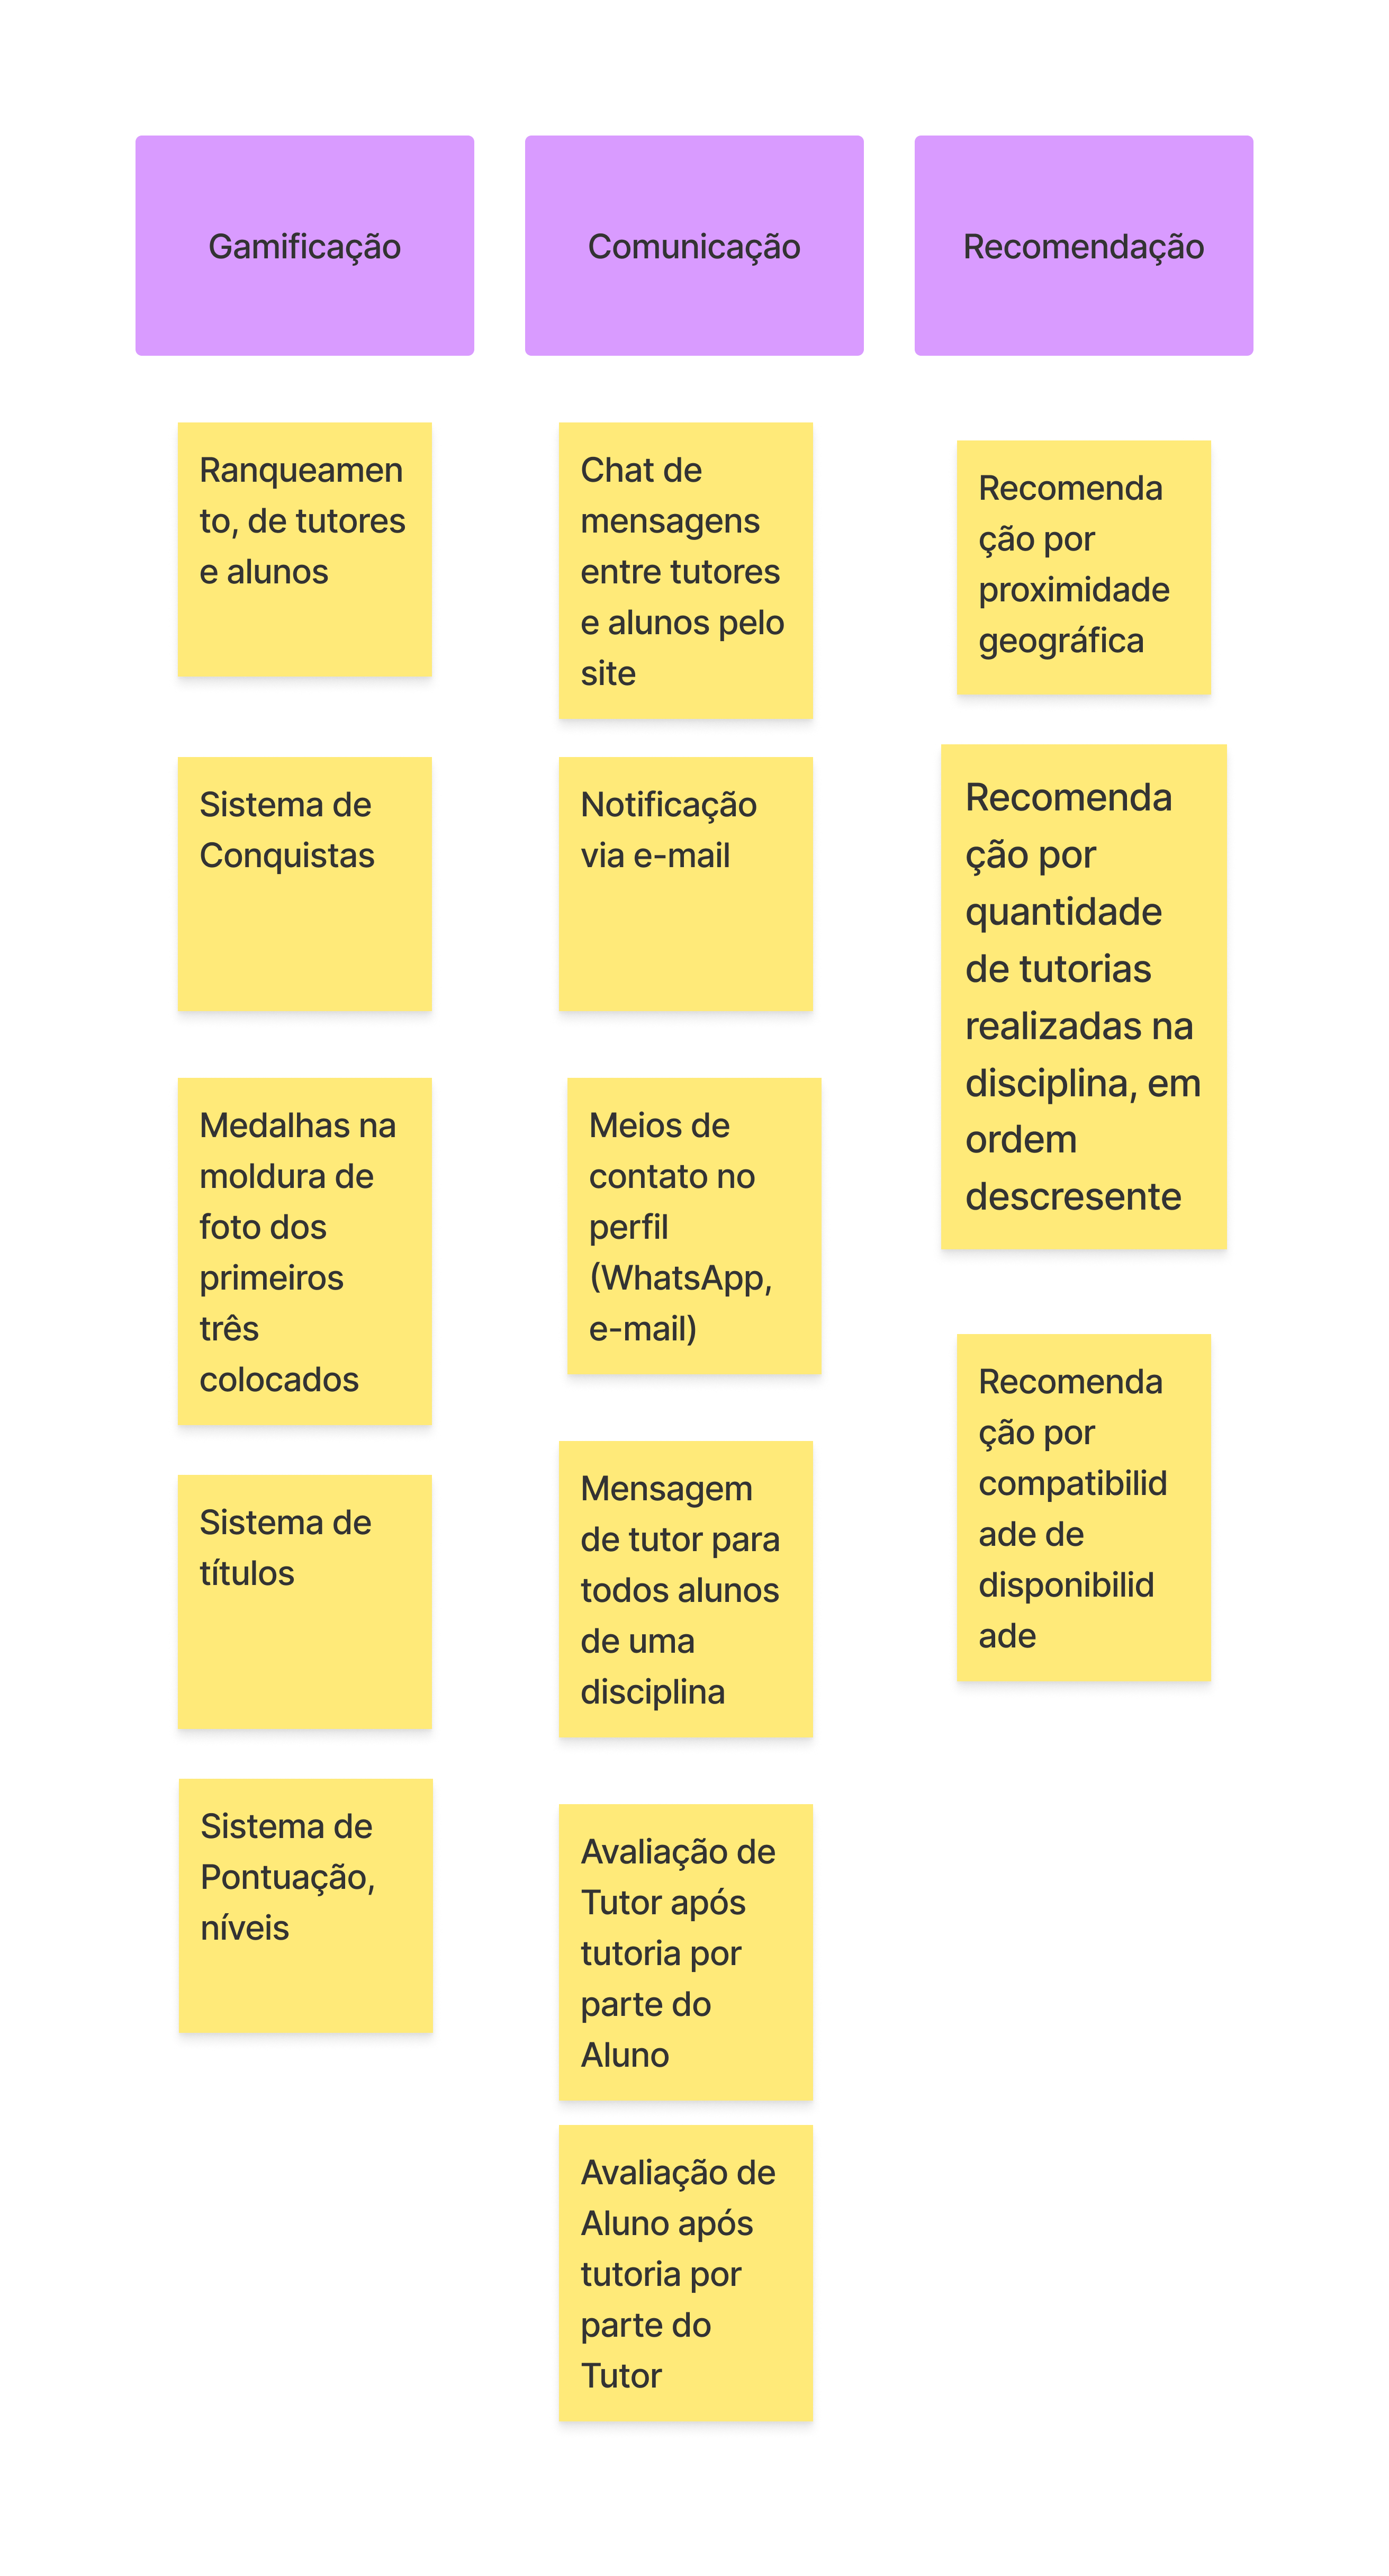
\includegraphics[width=0.7\textwidth]{figuras/Lean03Ideacao2.png}

    Fonte: Adaptado a partir de caroli.org
    
    \vspace{0.2cm}
\end{figure}

\begin{figure}[h!]
    \centering
    \caption{Ideias de funcionalidades (CRUDs).} 
    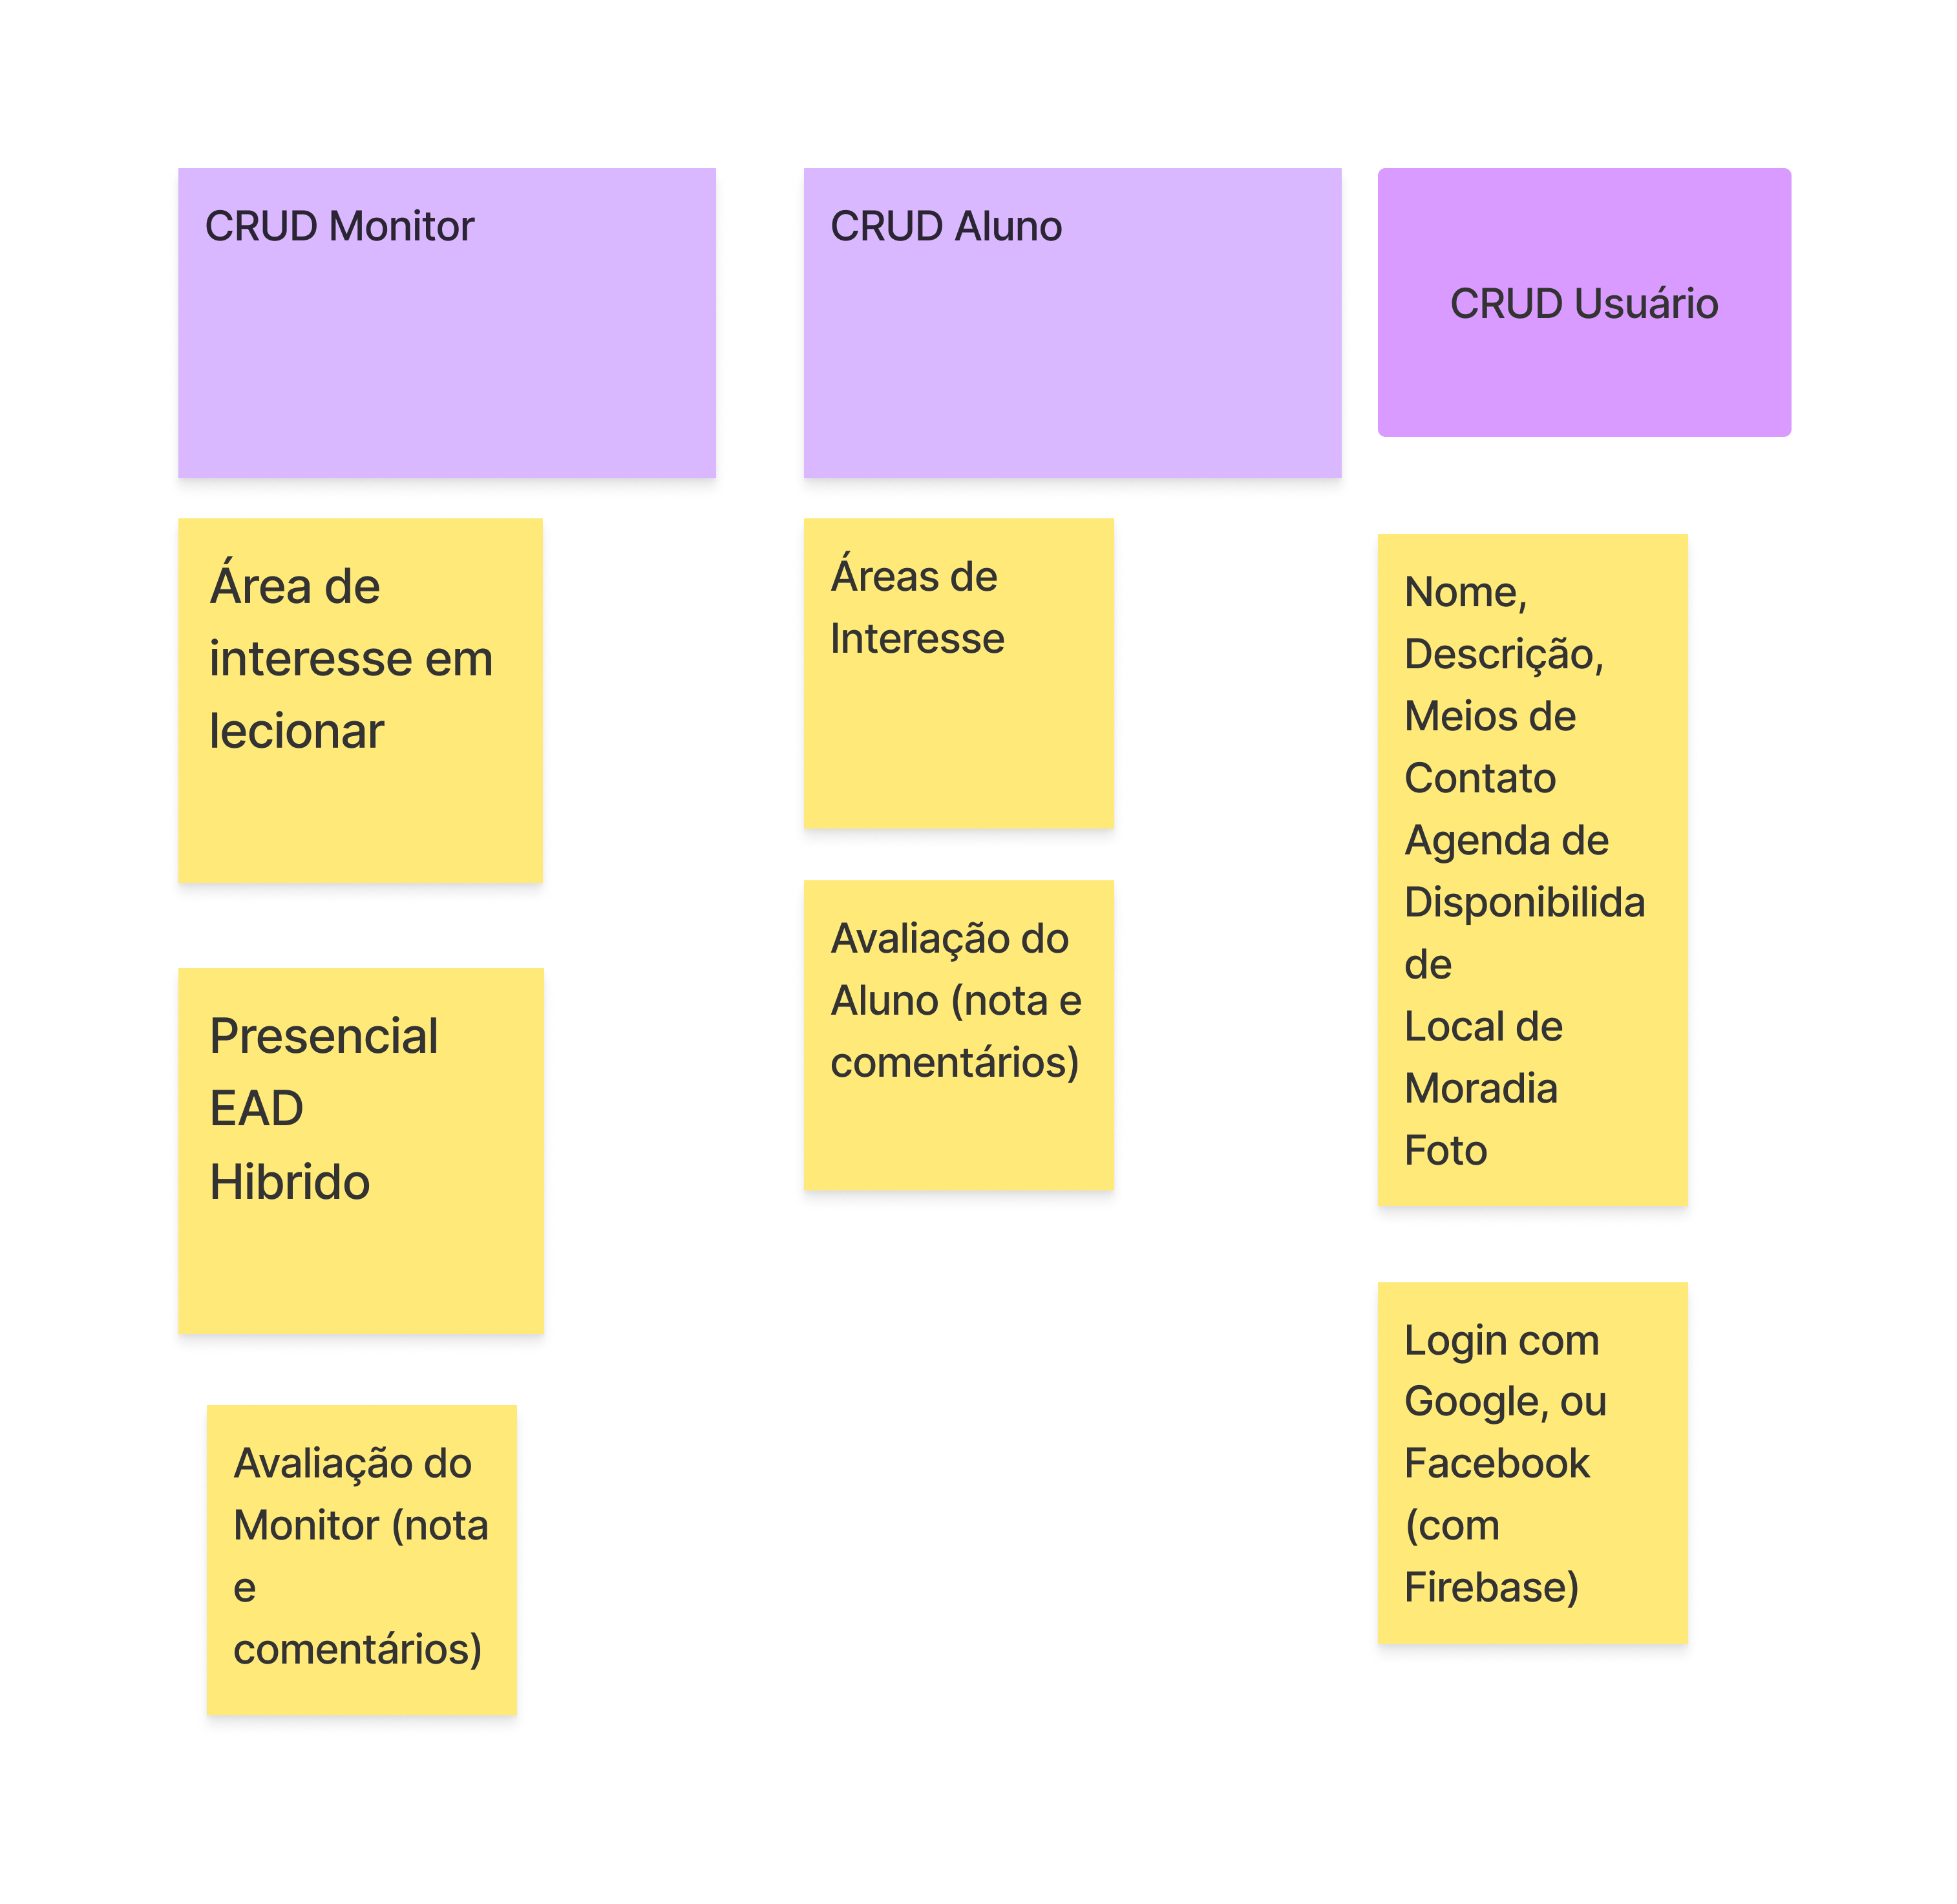
\includegraphics[width=0.9\textwidth]{figuras/Lean03Ideacao3.png}
    

    Fonte: Adaptado a partir de caroli.org
    
    \vspace{0.2cm}
\end{figure}

\begin{figure}[h!]
    \centering
    \caption{Persona do Aprendiz.} 
    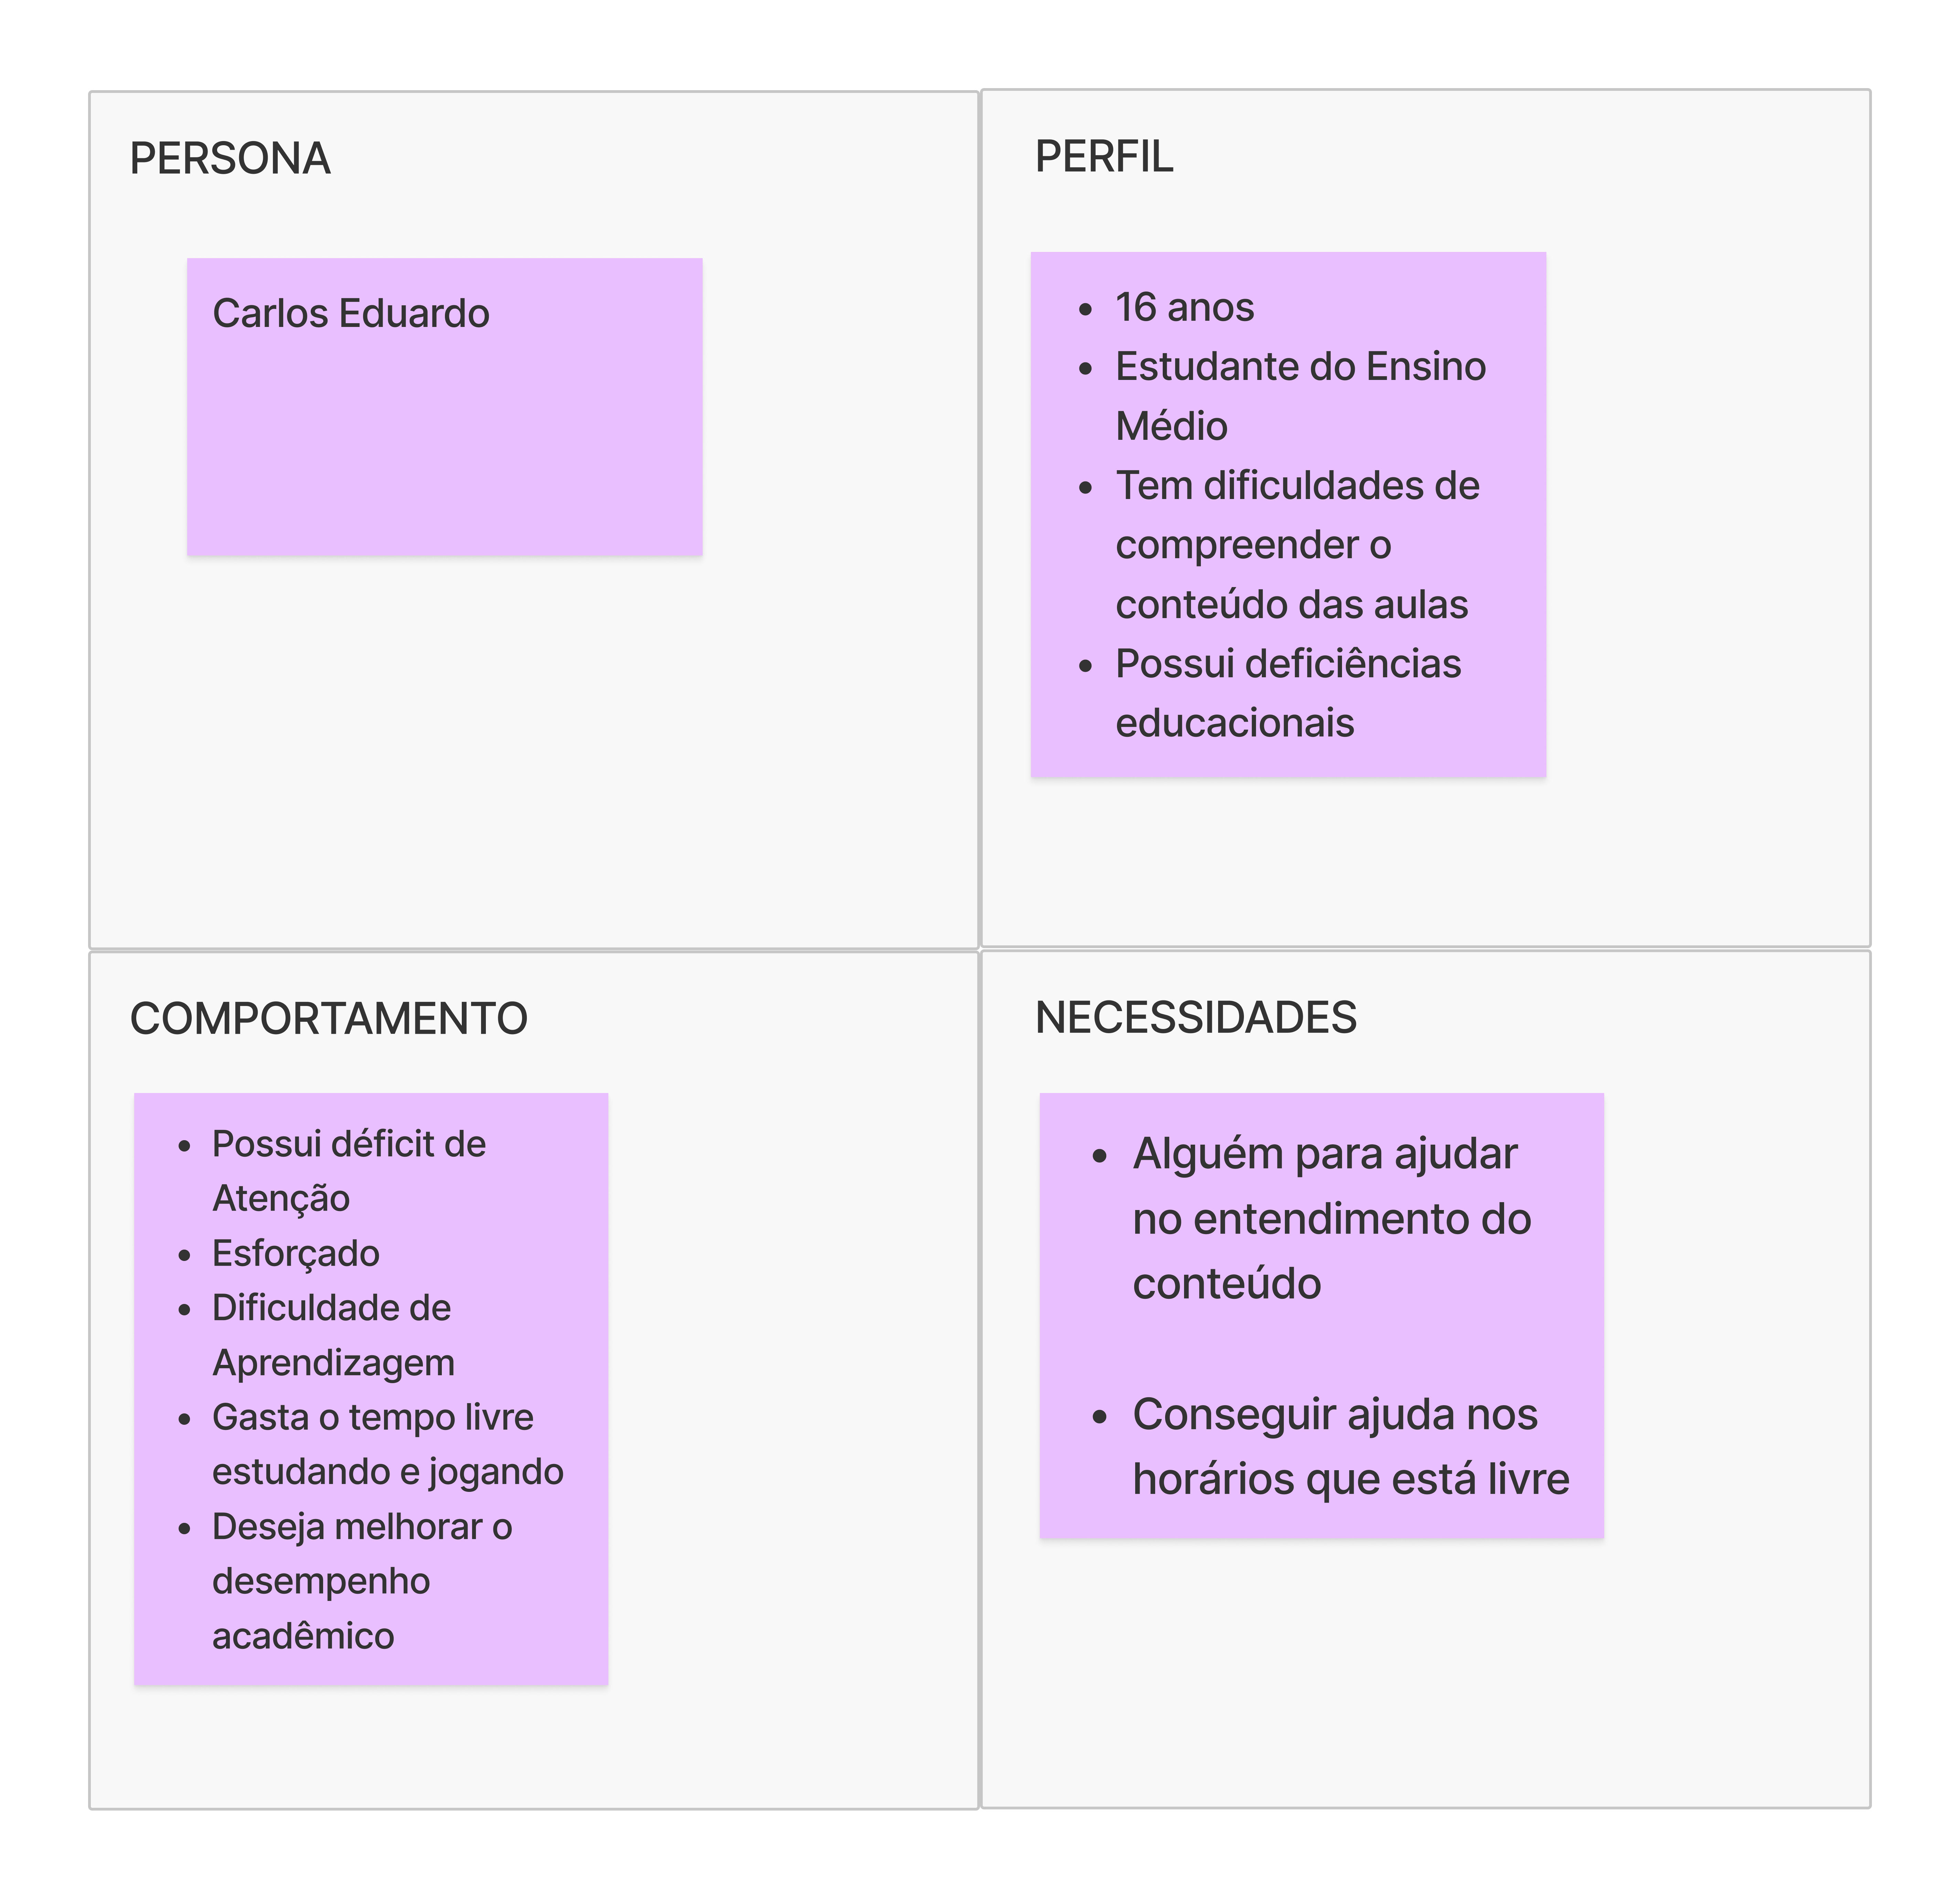
\includegraphics[width=0.9\textwidth]{figuras/Lean04Persona1.png}

    Fonte: Adaptado a partir de caroli.org
    
    \vspace{0.2cm}
\end{figure}

\begin{figure}[h!]
    \centering
    \caption{Persona do Tutor.} 
    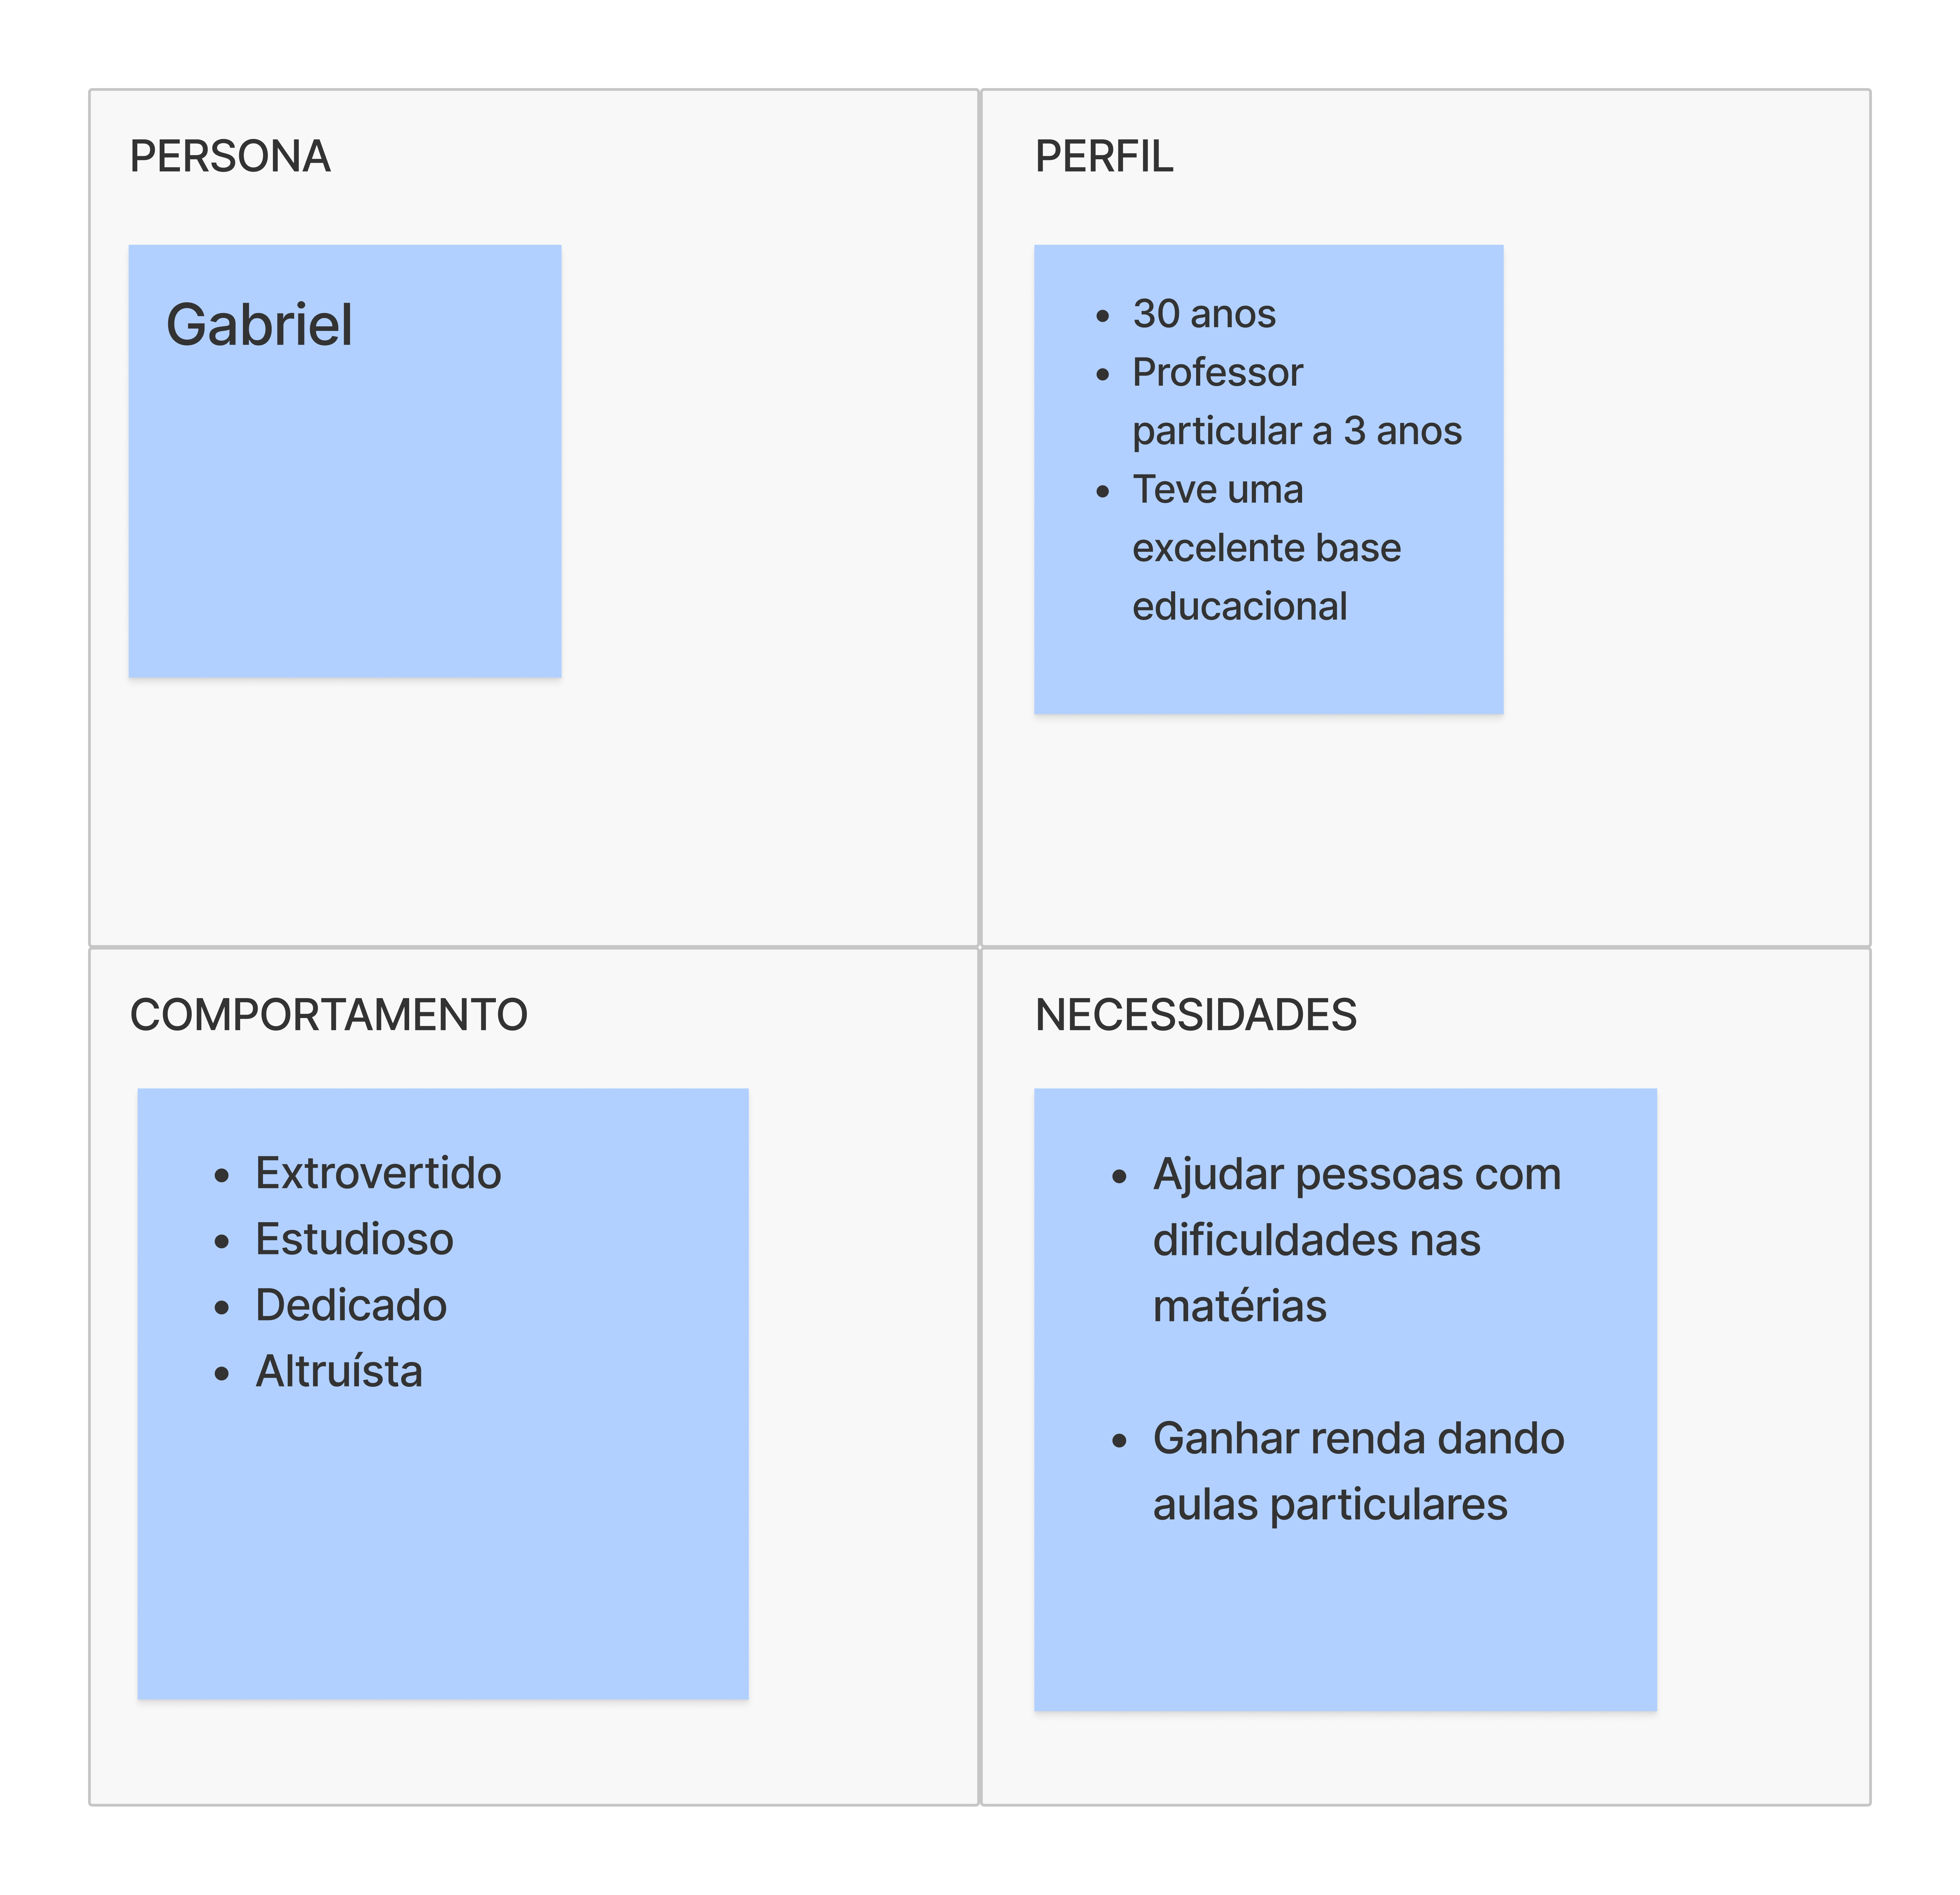
\includegraphics[width=0.9\textwidth]{figuras/Lean05Persona2.png}

    Fonte: Adaptado a partir de caroli.org
    
    \vspace{0.2cm}
\end{figure}

% \begin{figure}[h!]
%     \centering
%     \caption{Persona 3.} 
%     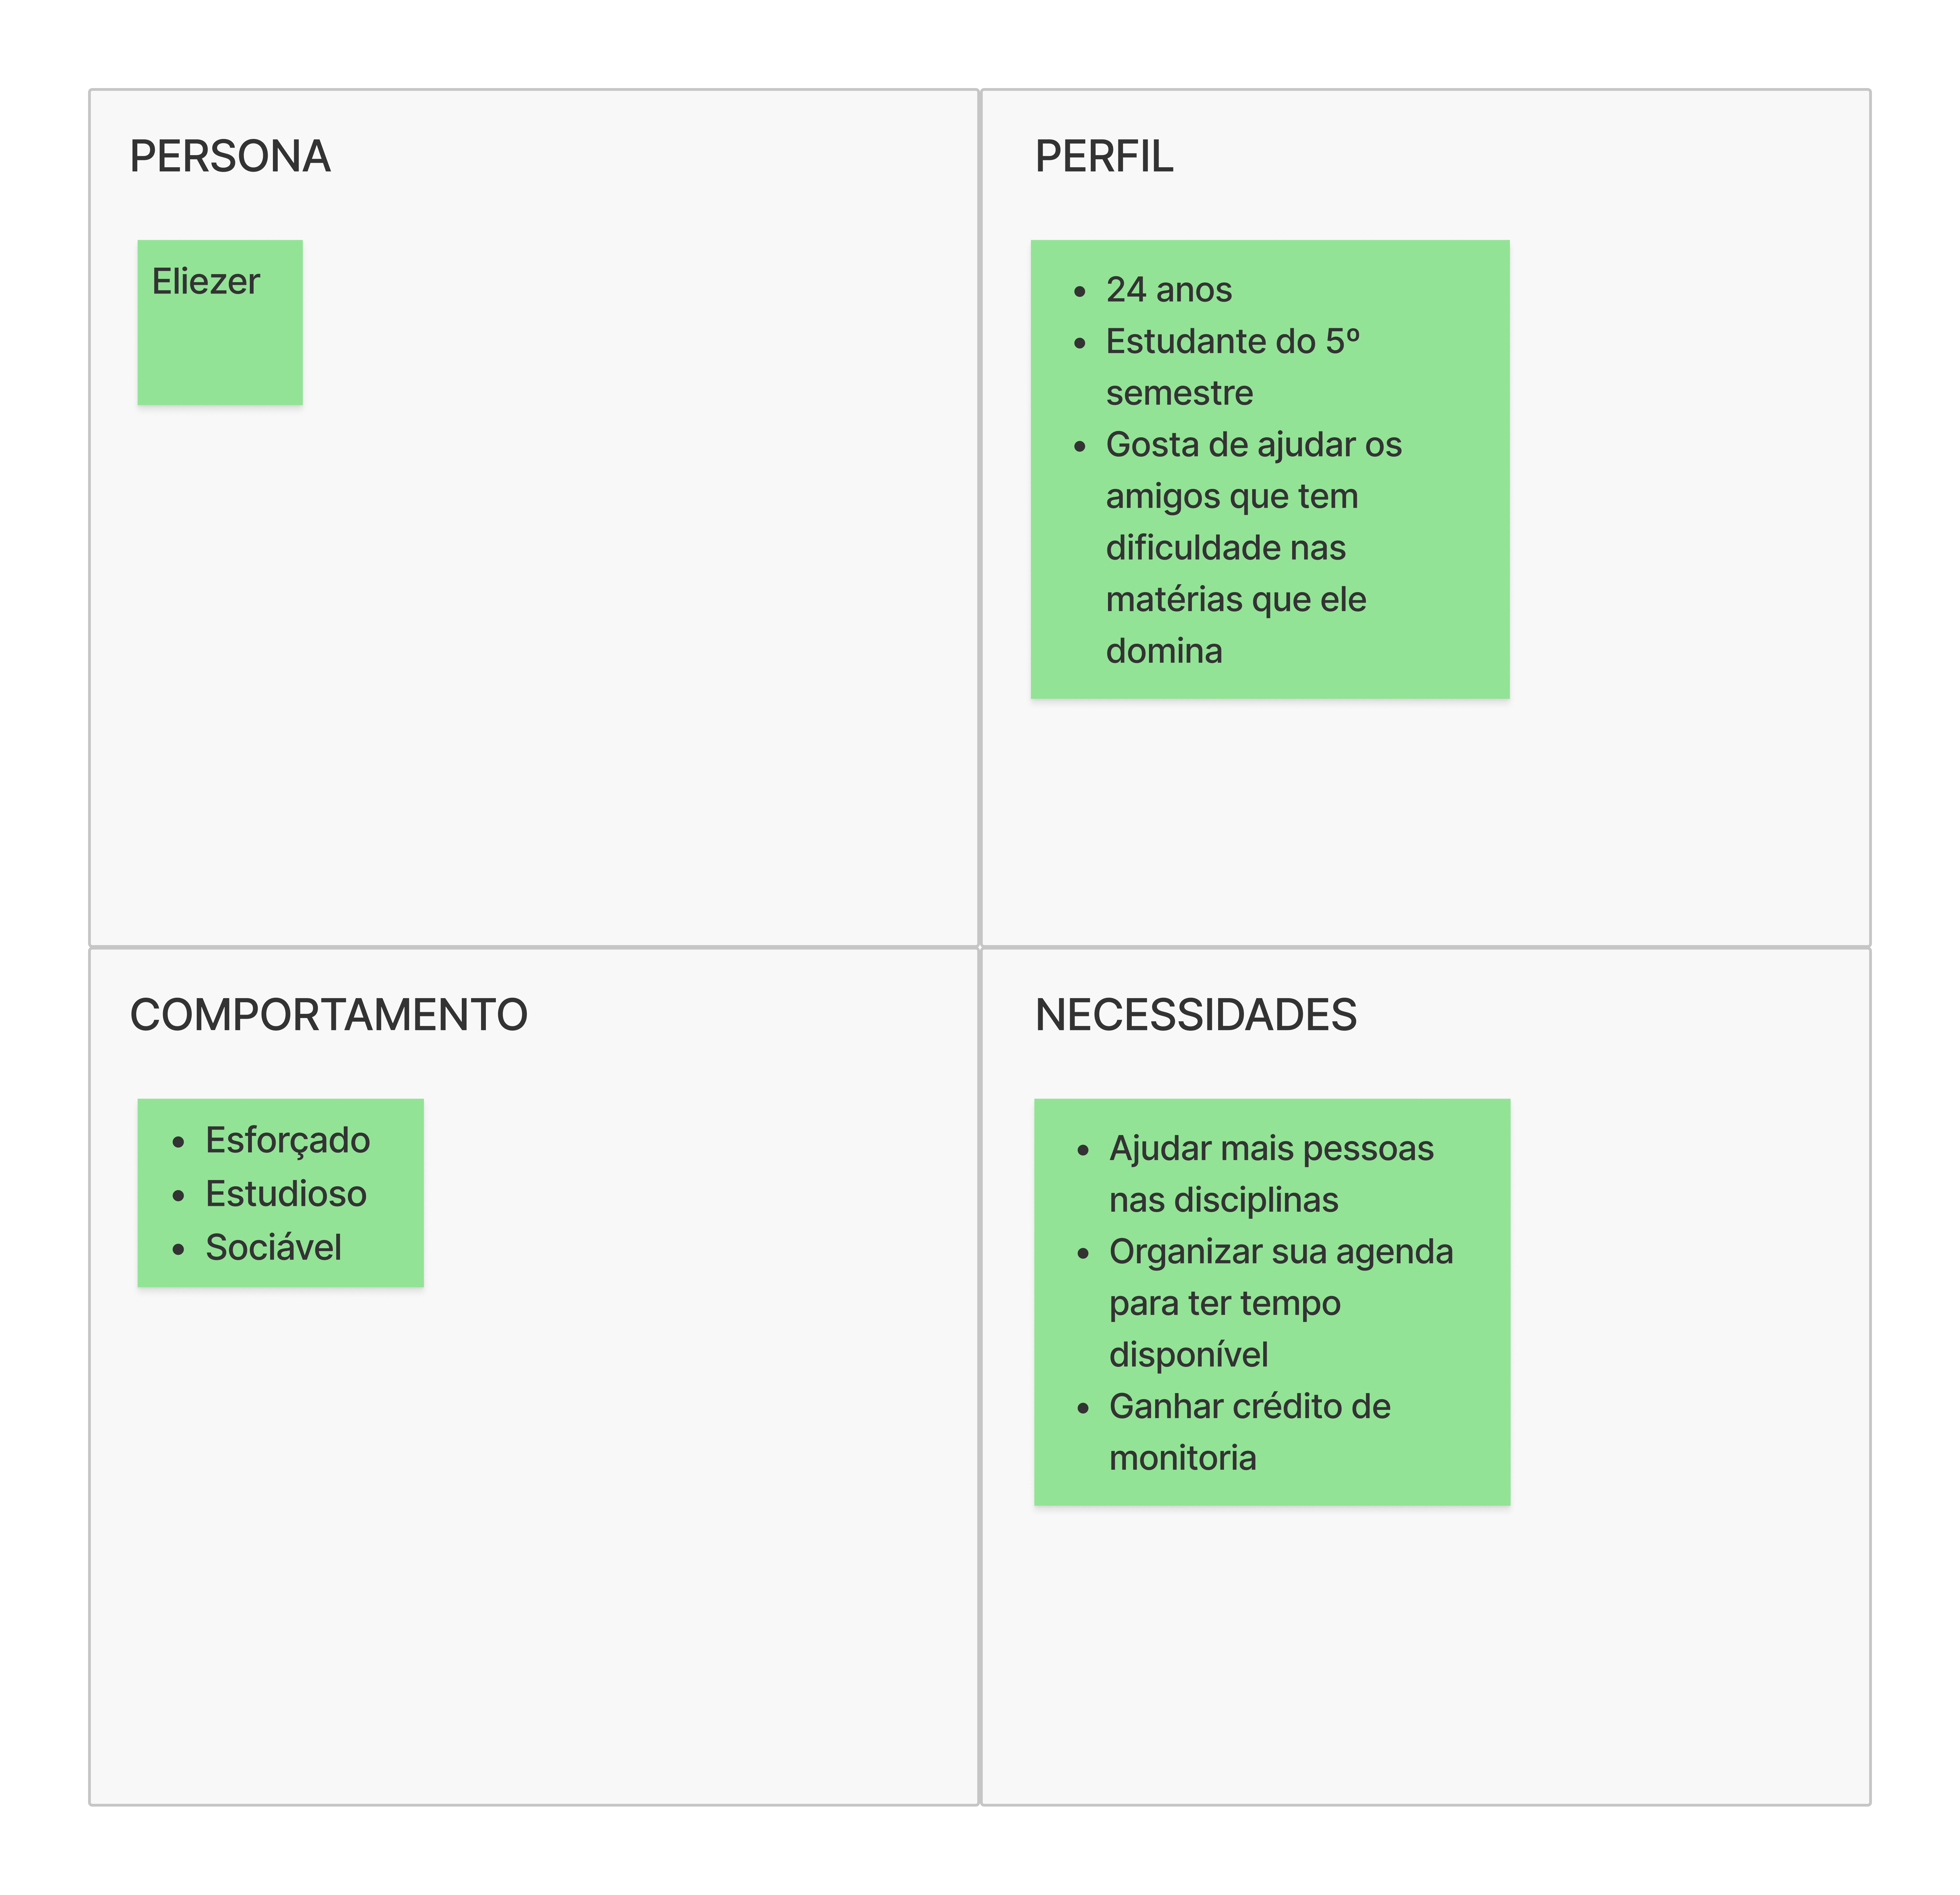
\includegraphics[width=0.9\textwidth]{figuras/Lean06Persona3.png}

%     Fonte: Adaptada a partir de caroli.org
    
%     \vspace{0.2cm}
% \end{figure}

% \begin{figure}[h!]
%     \centering
%     \caption{Persona 1.} 
%     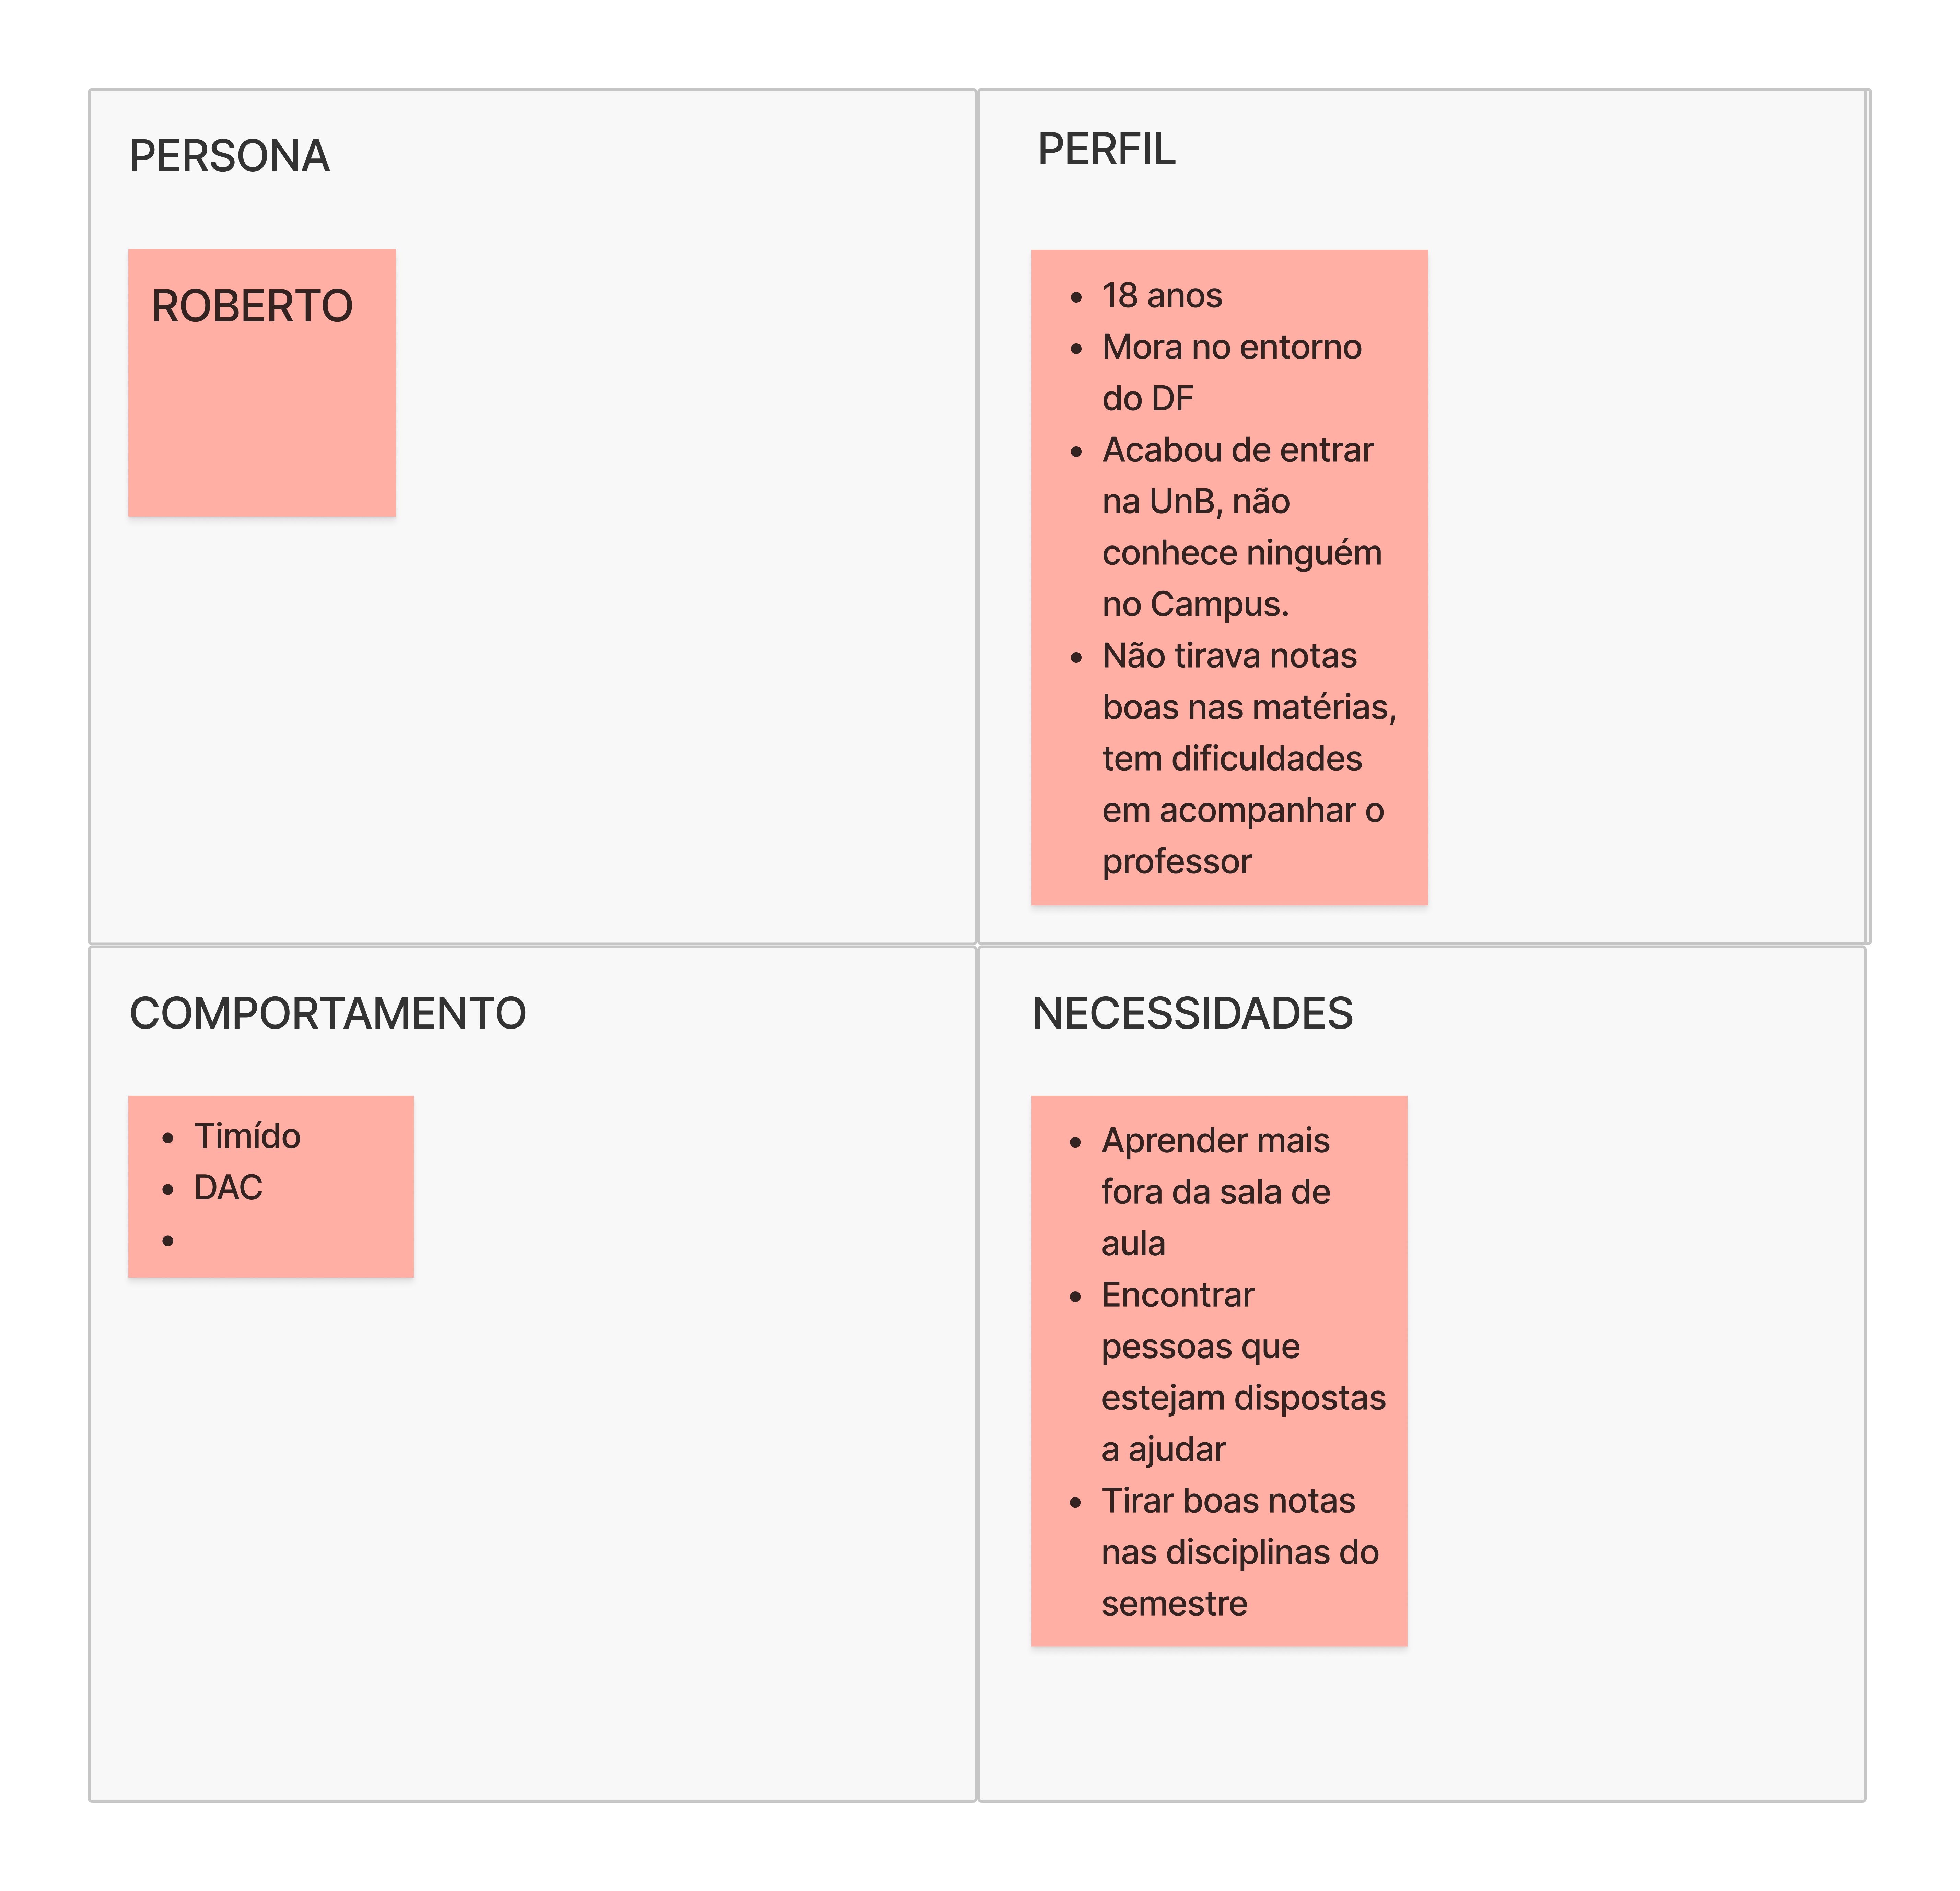
\includegraphics[width=0.9\textwidth]{figuras/Lean07Persona4.png}

%     Fonte: Adaptada a partir de caroli.org
    
%     \vspace{0.2cm}
% \end{figure}

\begin{figure}[h!]
    \centering
    \caption{Jornada do Aprendiz.} 
    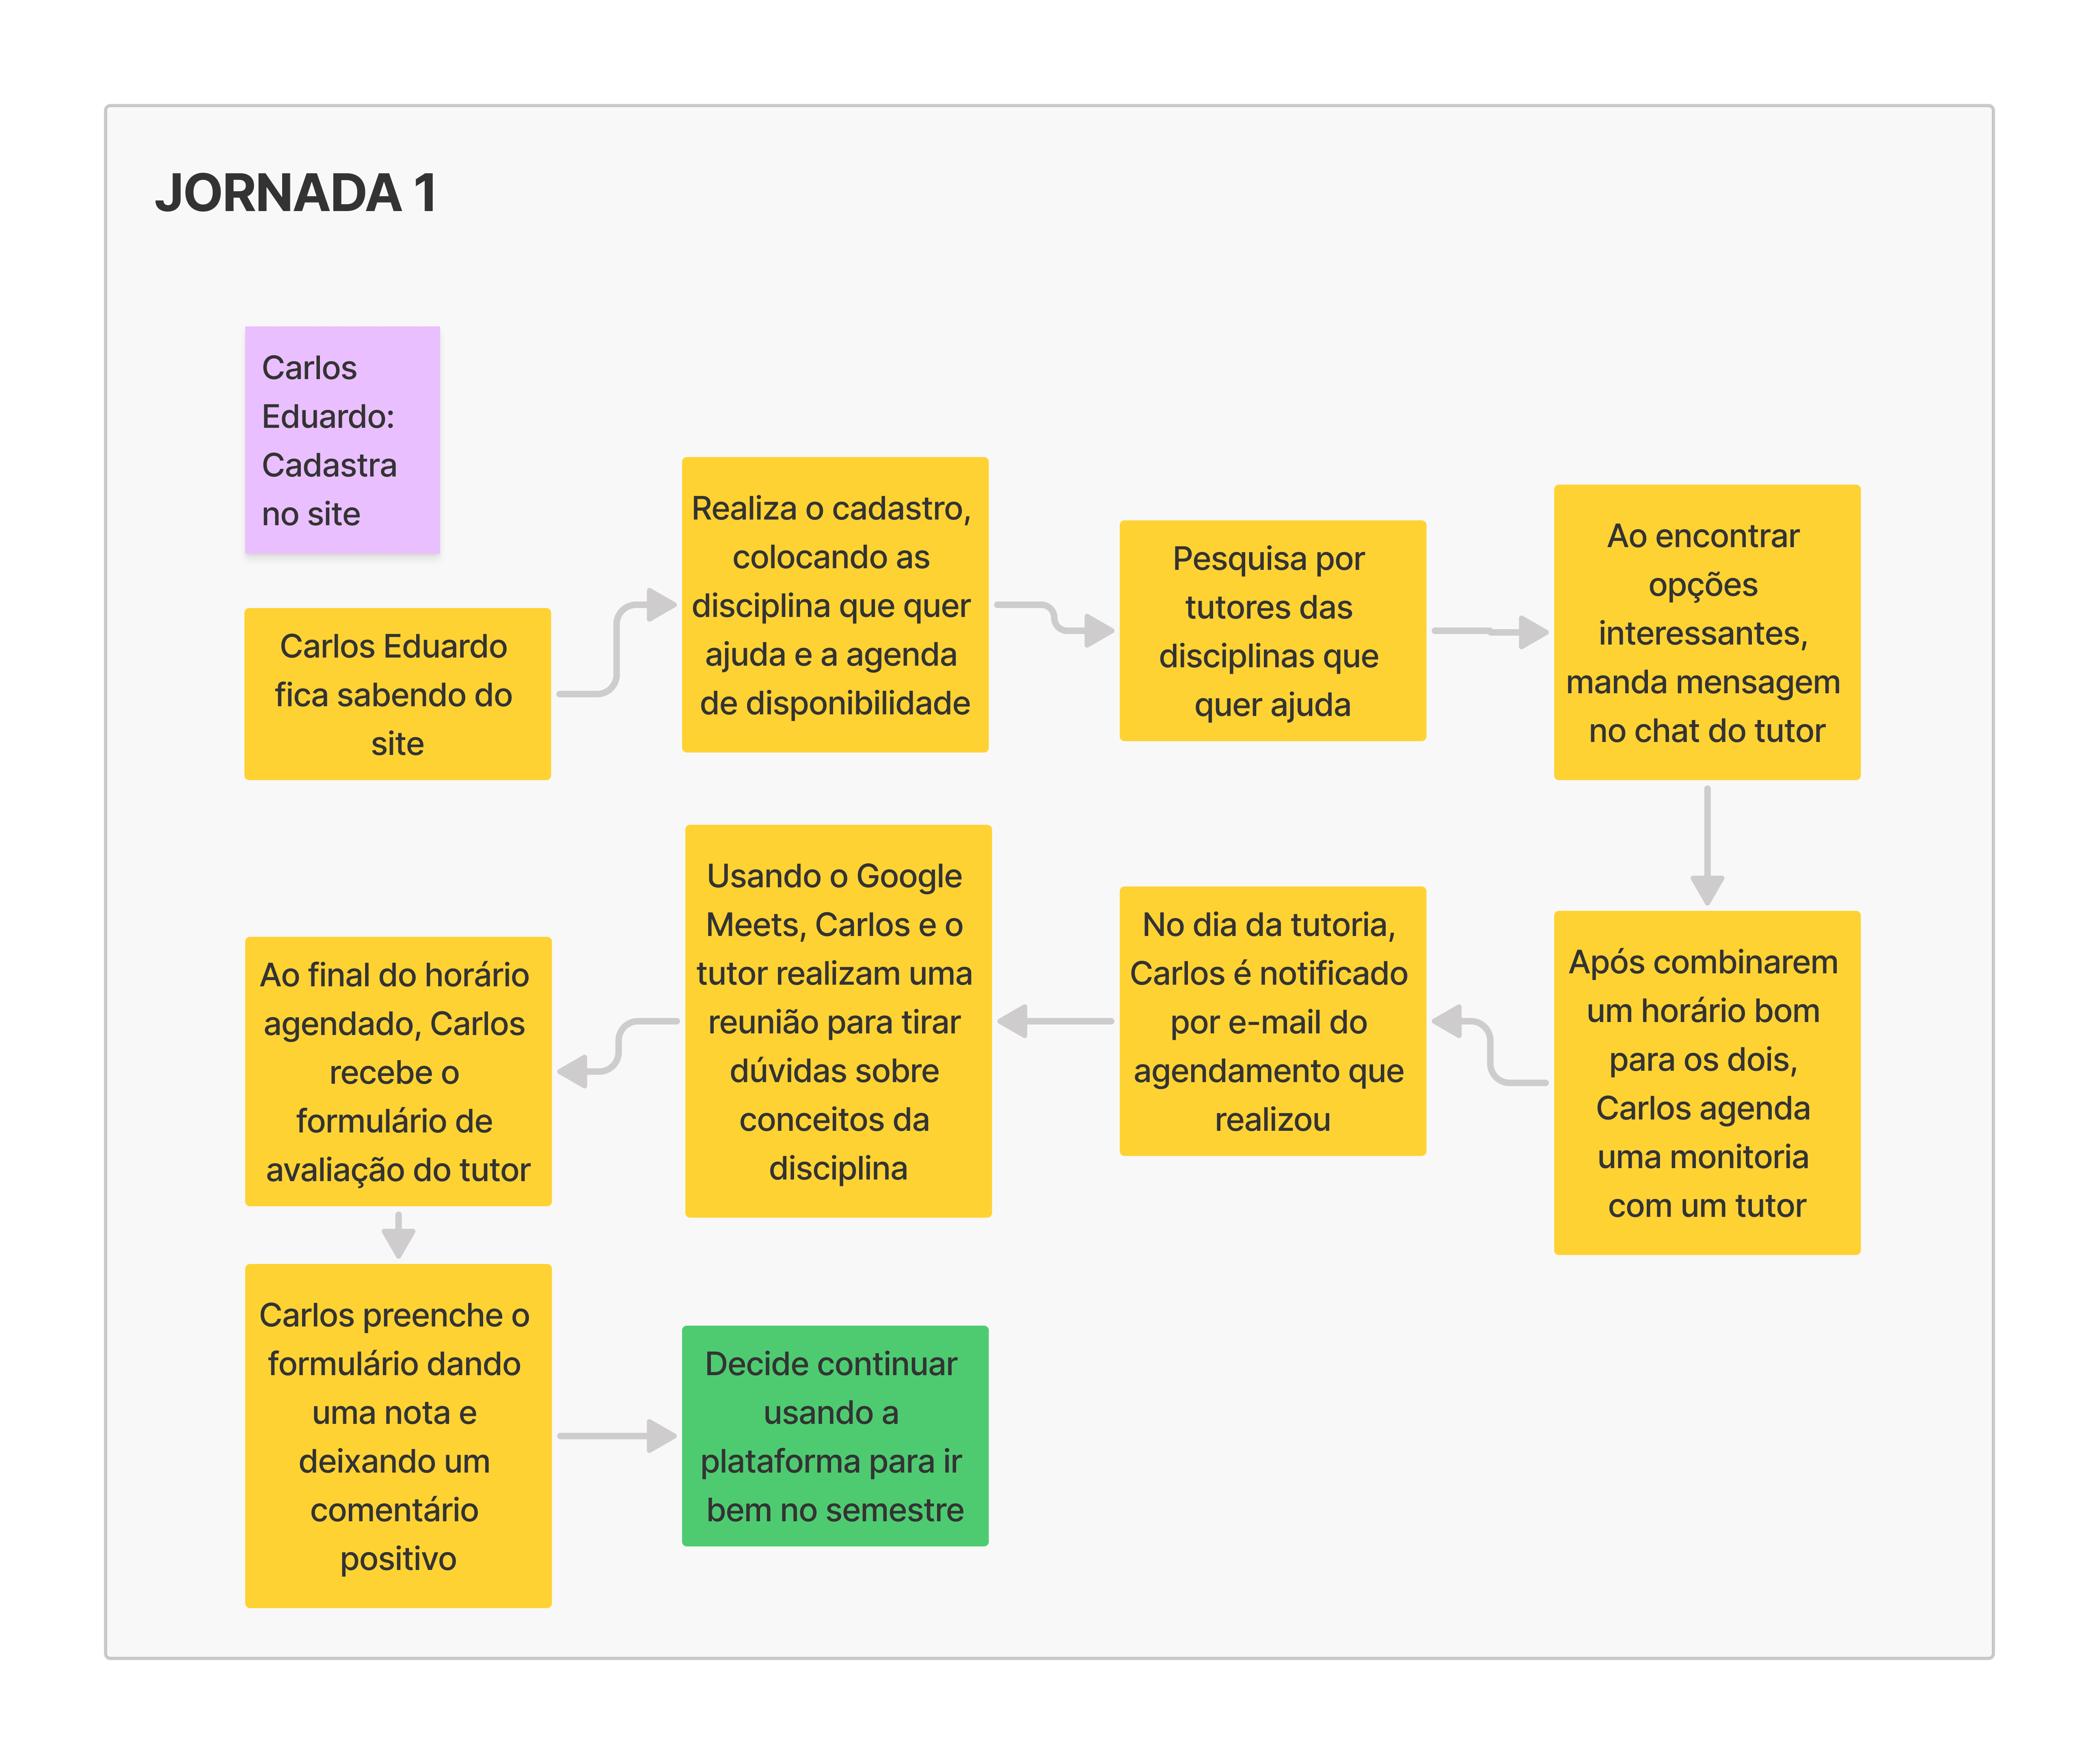
\includegraphics[width=1\textwidth]{figuras/Lean08Jornada1.png}

    Fonte: Adaptado a partir de caroli.org
    
    \vspace{0.2cm}
\end{figure}

\begin{figure}[h!]
    \centering
    \caption{\textit{Brainstorm} de Funcionalidades.} 
    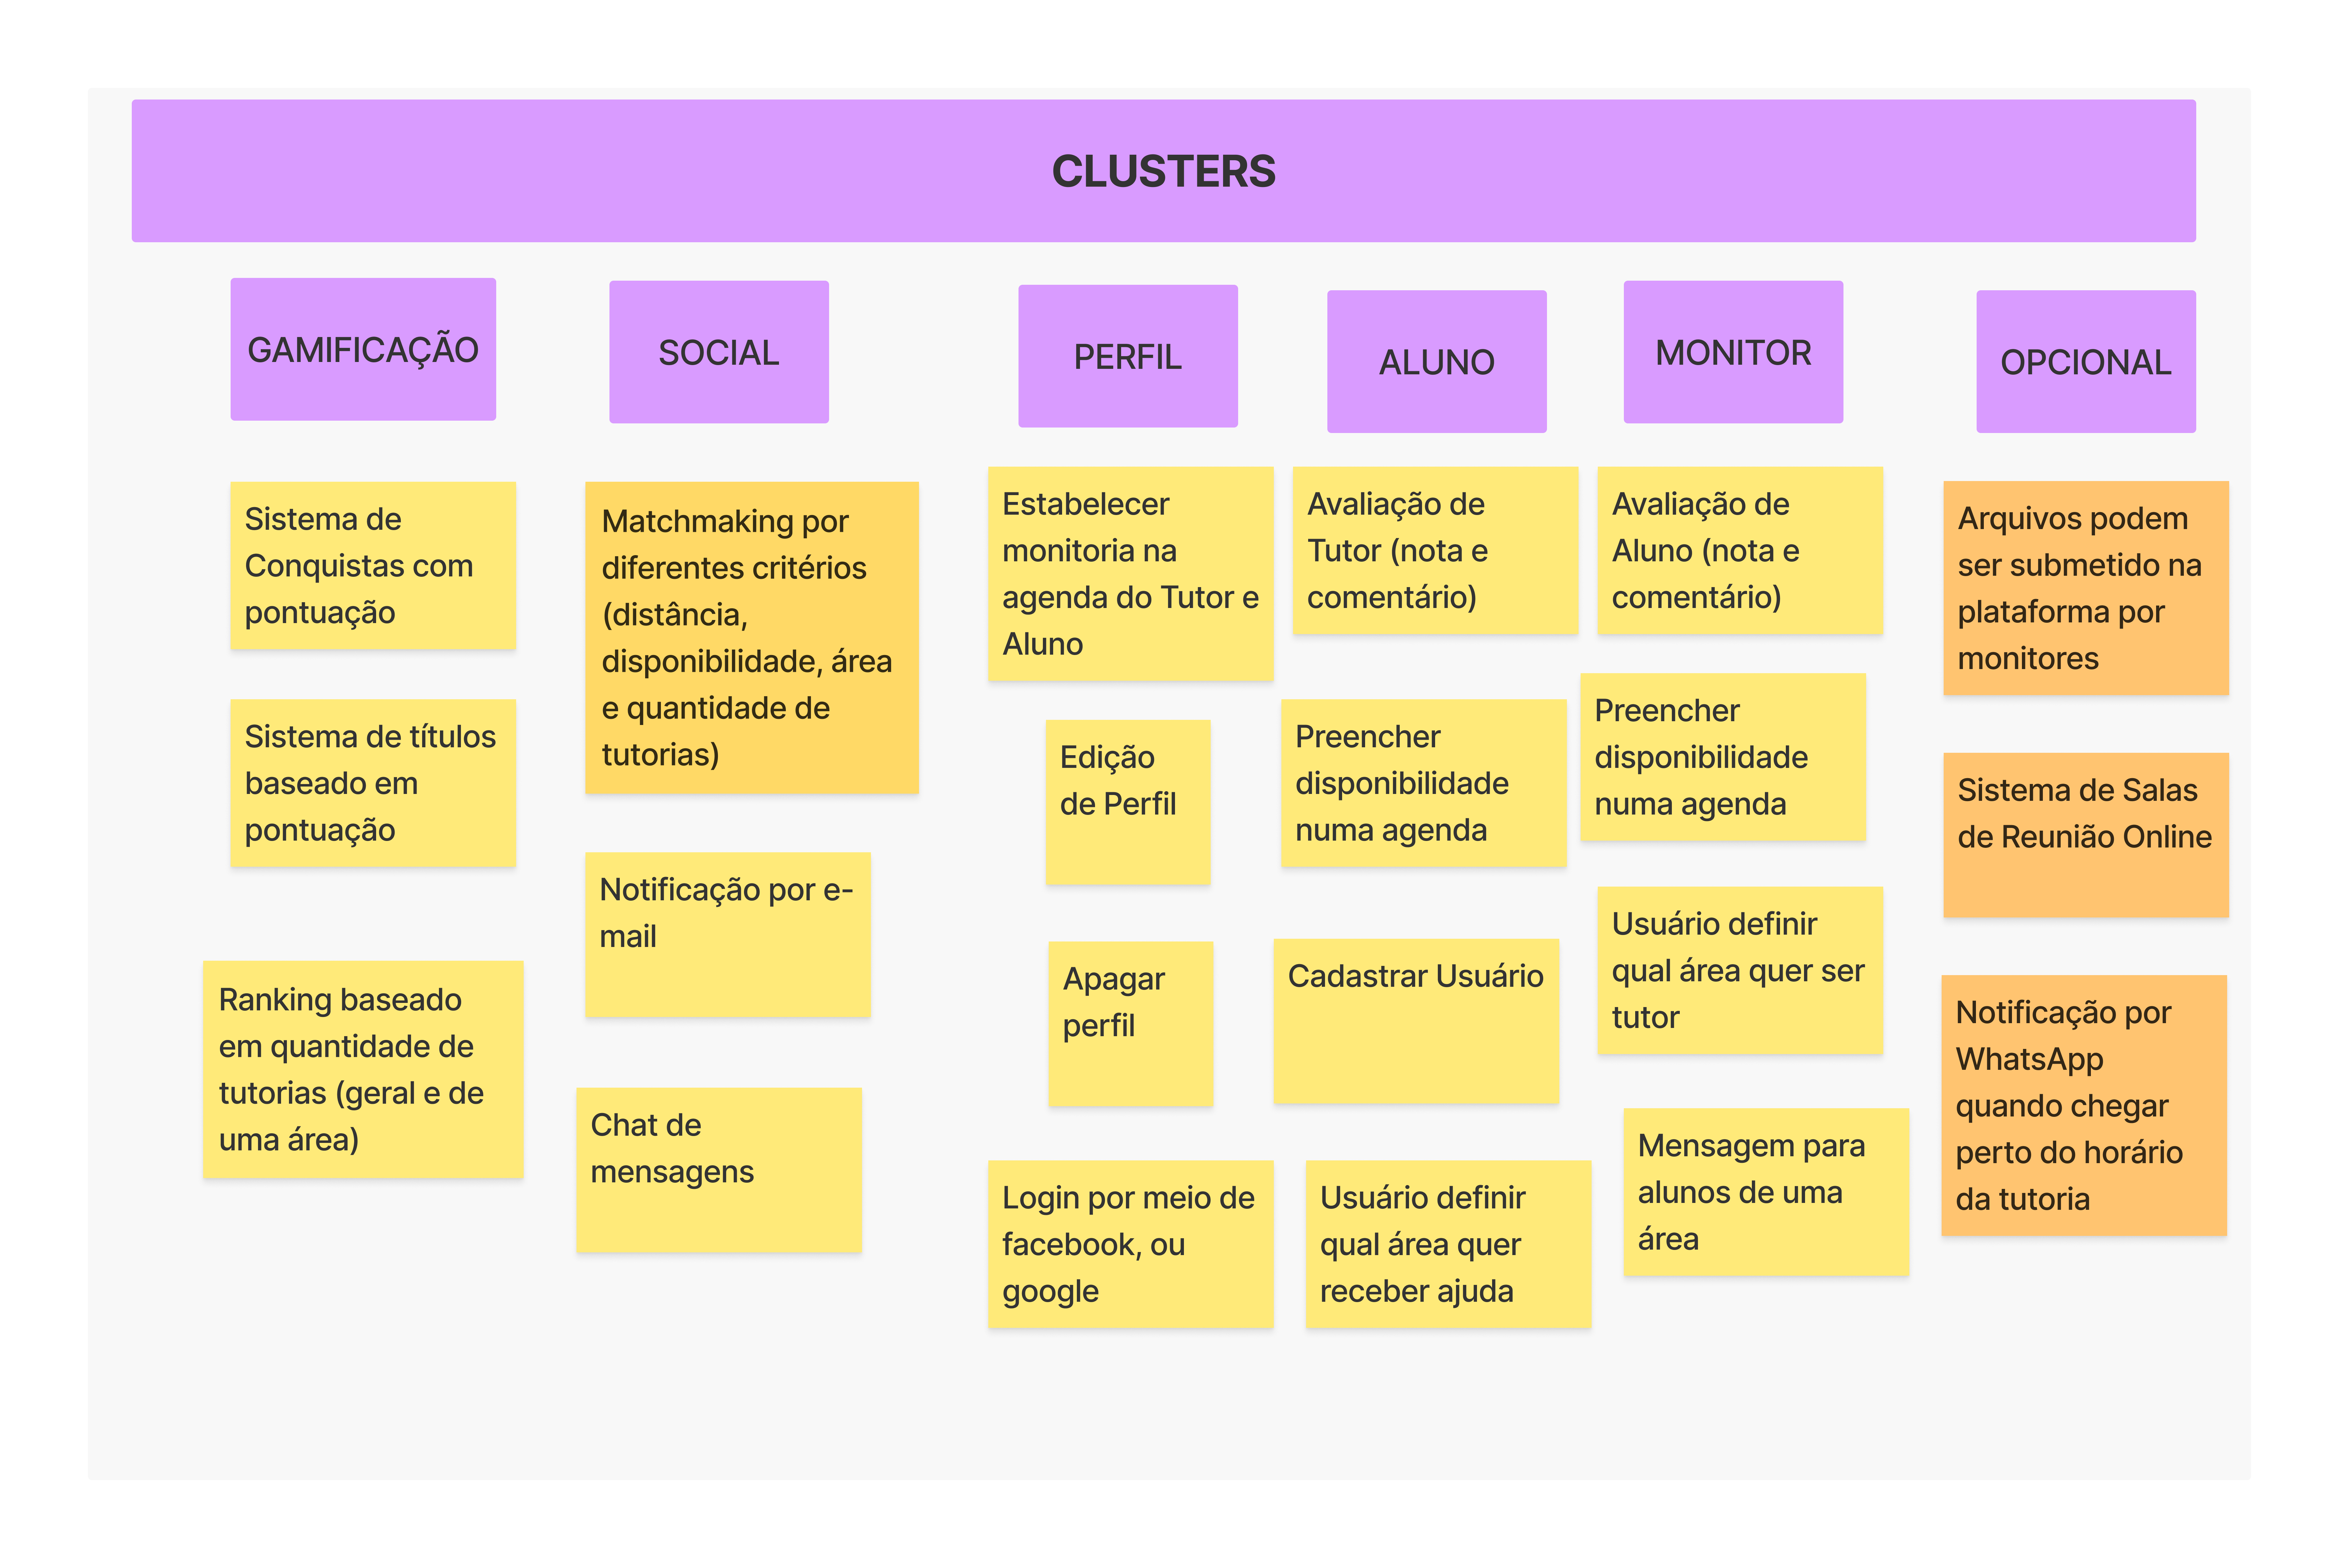
\includegraphics[width=1\textwidth]{figuras/Lean12Funcionalidades.png}

    Fonte: Adaptado a partir de caroli.org
    
    \vspace{0.2cm}
\end{figure}

\begin{figure}[h!]
    \centering
    \caption{Revisão técnica de negócio e de experiência de usuário (Gamificação, Social e Perfil).} 
    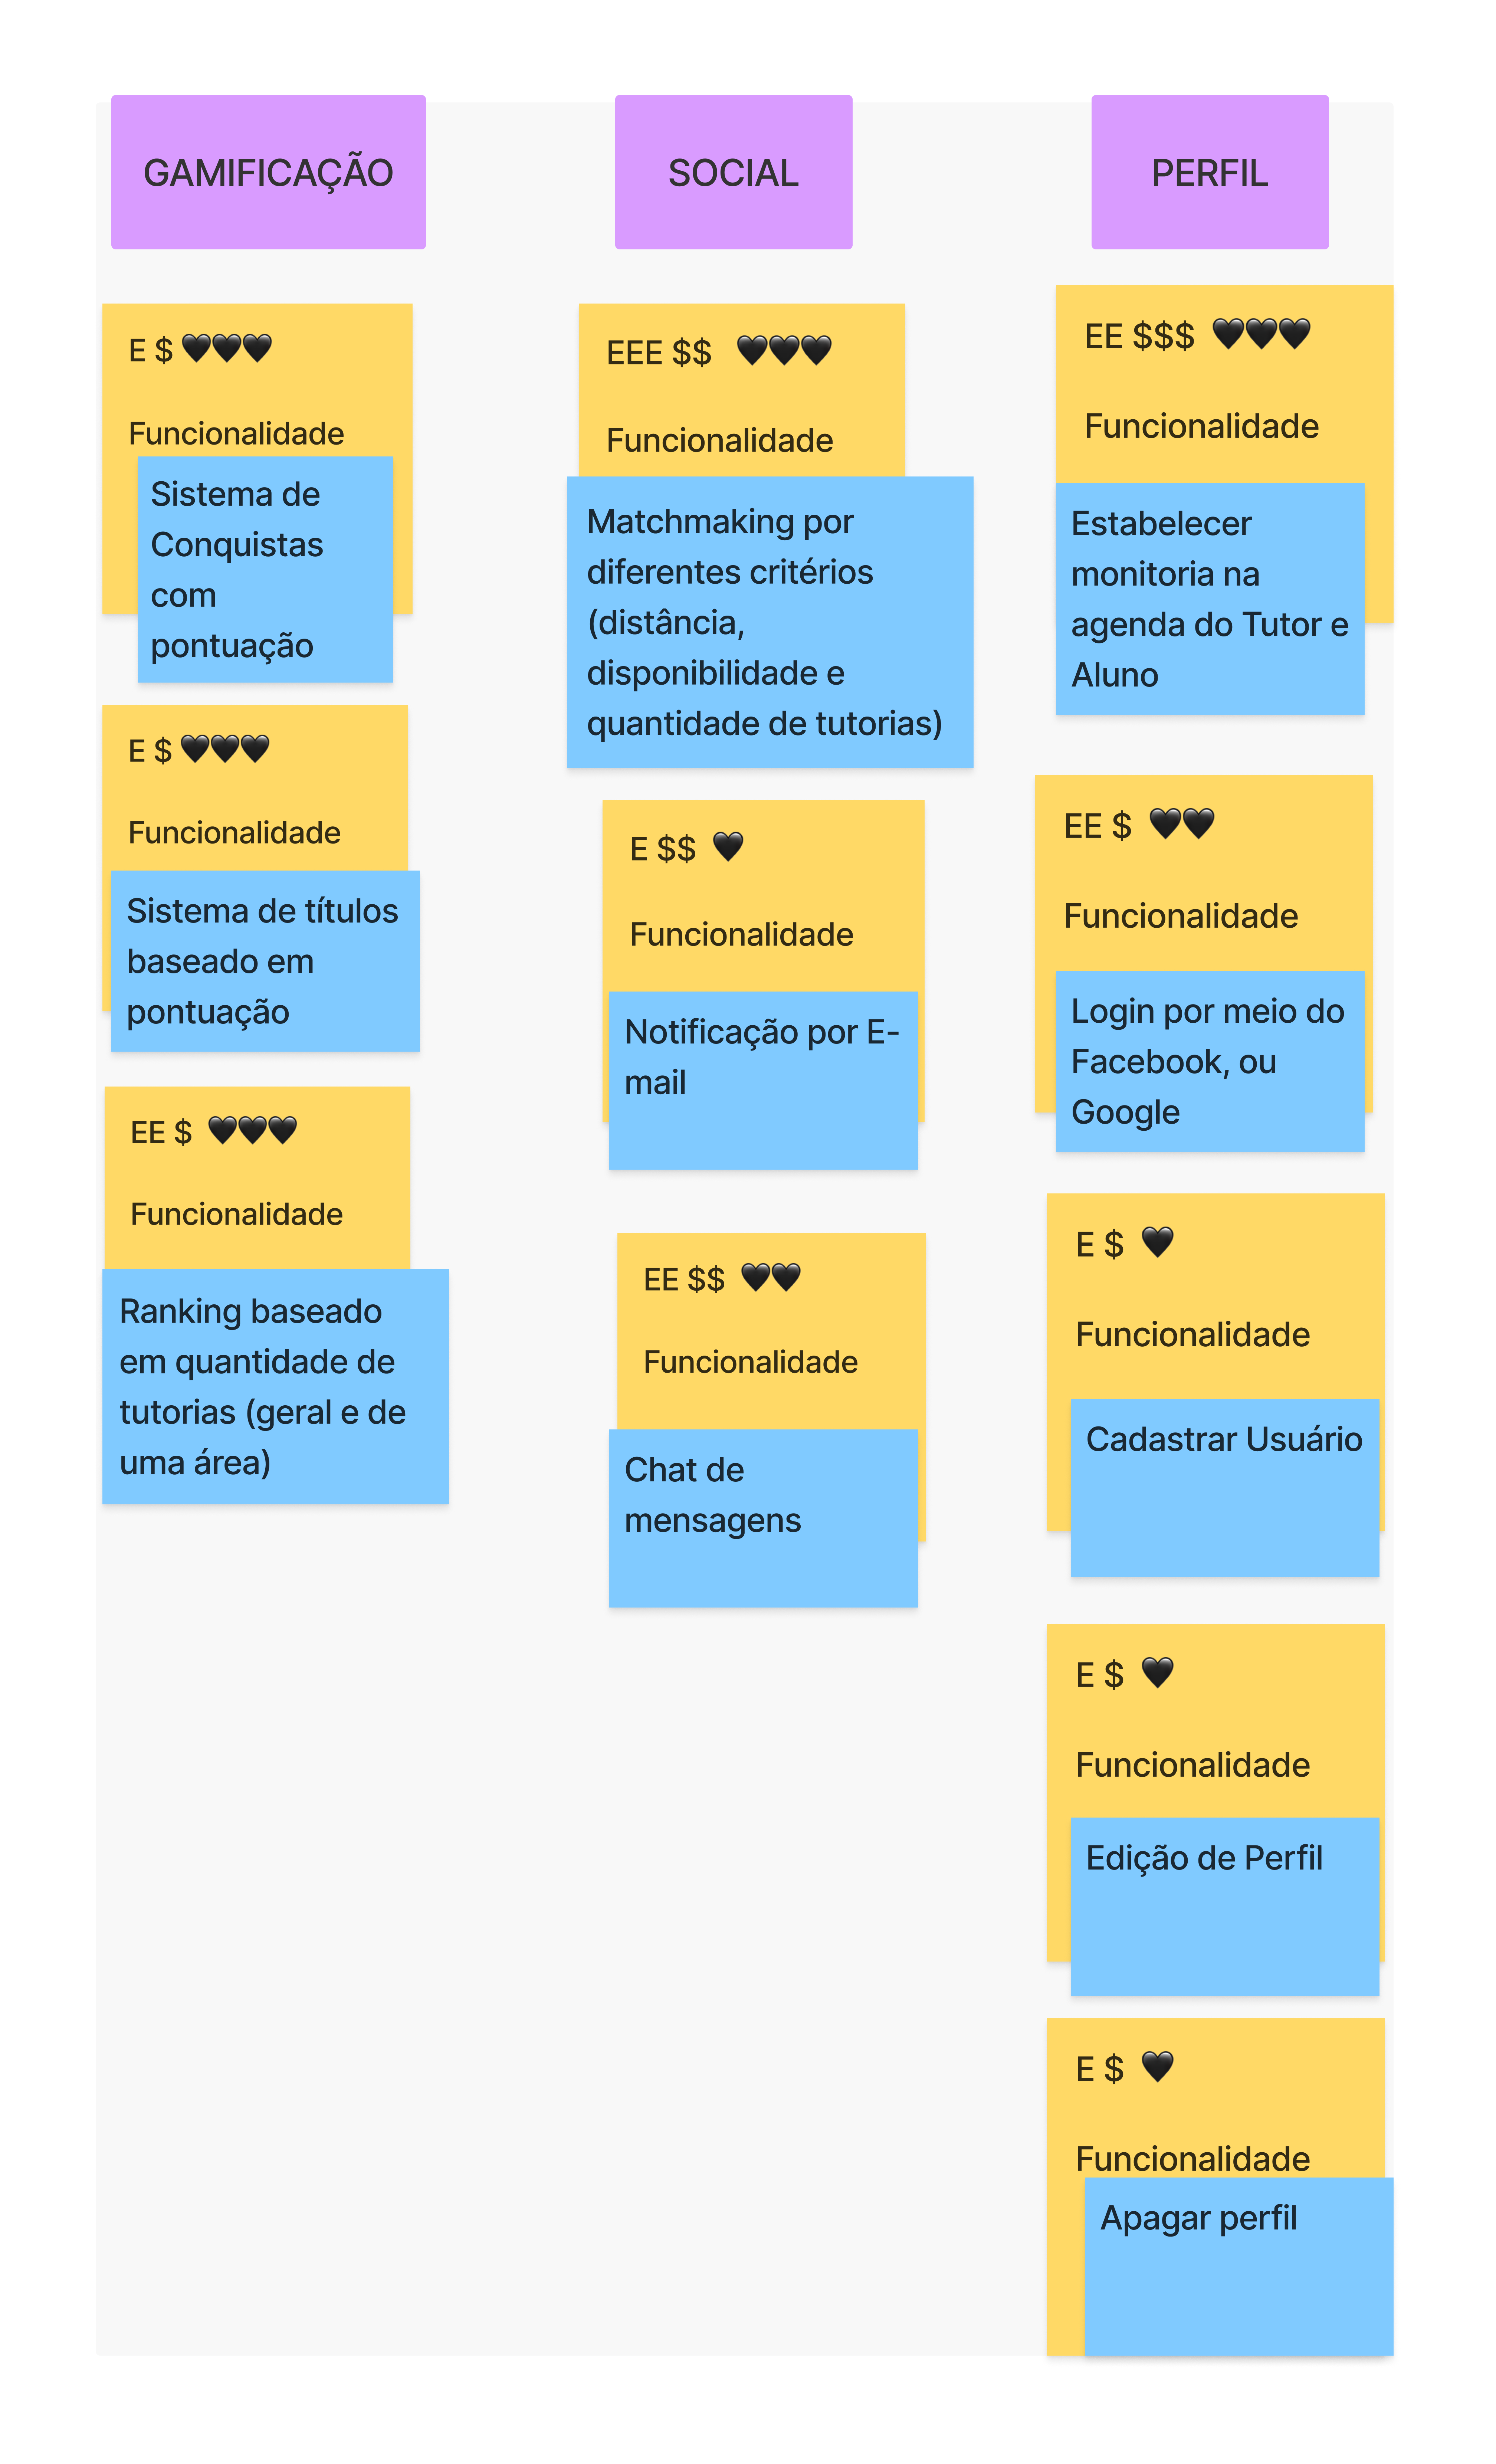
\includegraphics[width=0.7\textwidth]{figuras/Lean13Custos.png}

    Fonte: Adaptado a partir de caroli.org
    
    \vspace{0.2cm}
\end{figure}

\begin{figure}[h!]
    \centering
    \caption{Revisão técnica de negócio e de experiência de usuário (Aluno, Monitor e Opcional).} 
    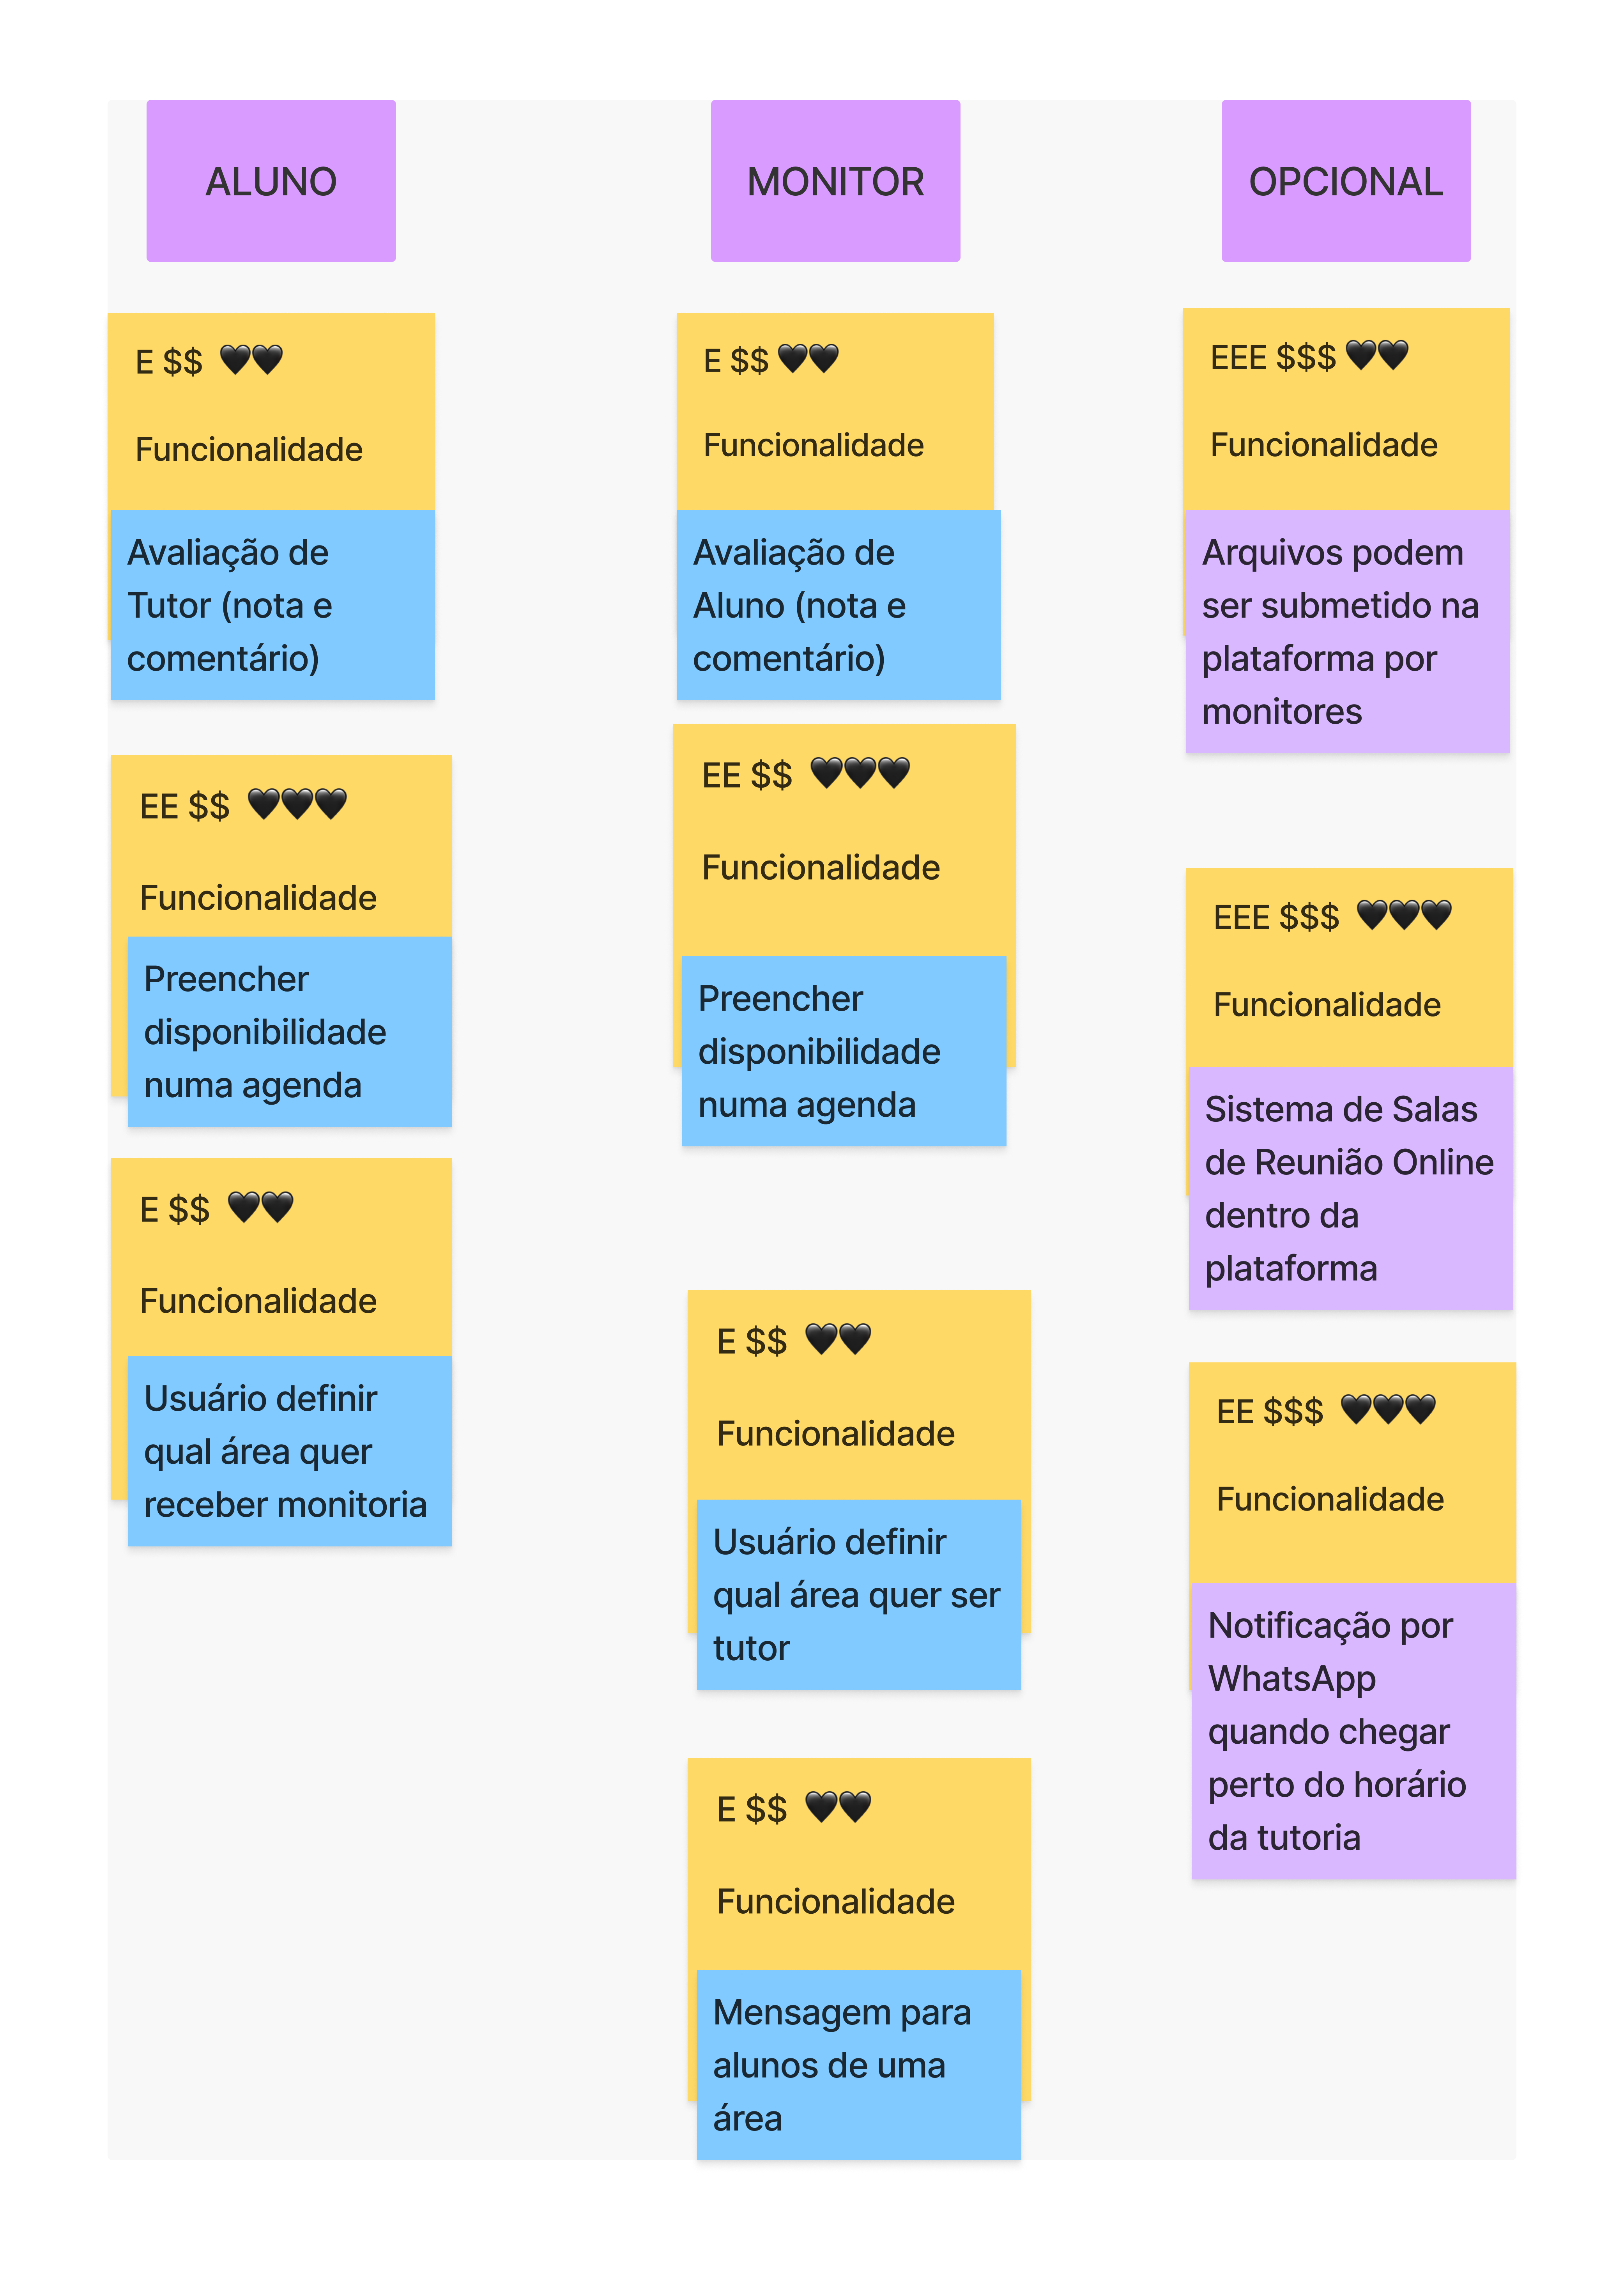
\includegraphics[width=0.7\textwidth]{figuras/Lean13Custos2.png}

    Fonte: Adaptado a partir de caroli.org
    
    \vspace{0.2cm}
\end{figure}

\begin{figure}[h!]
    \centering
    \caption{Sequenciador (quatro primeiros níveis).} 
    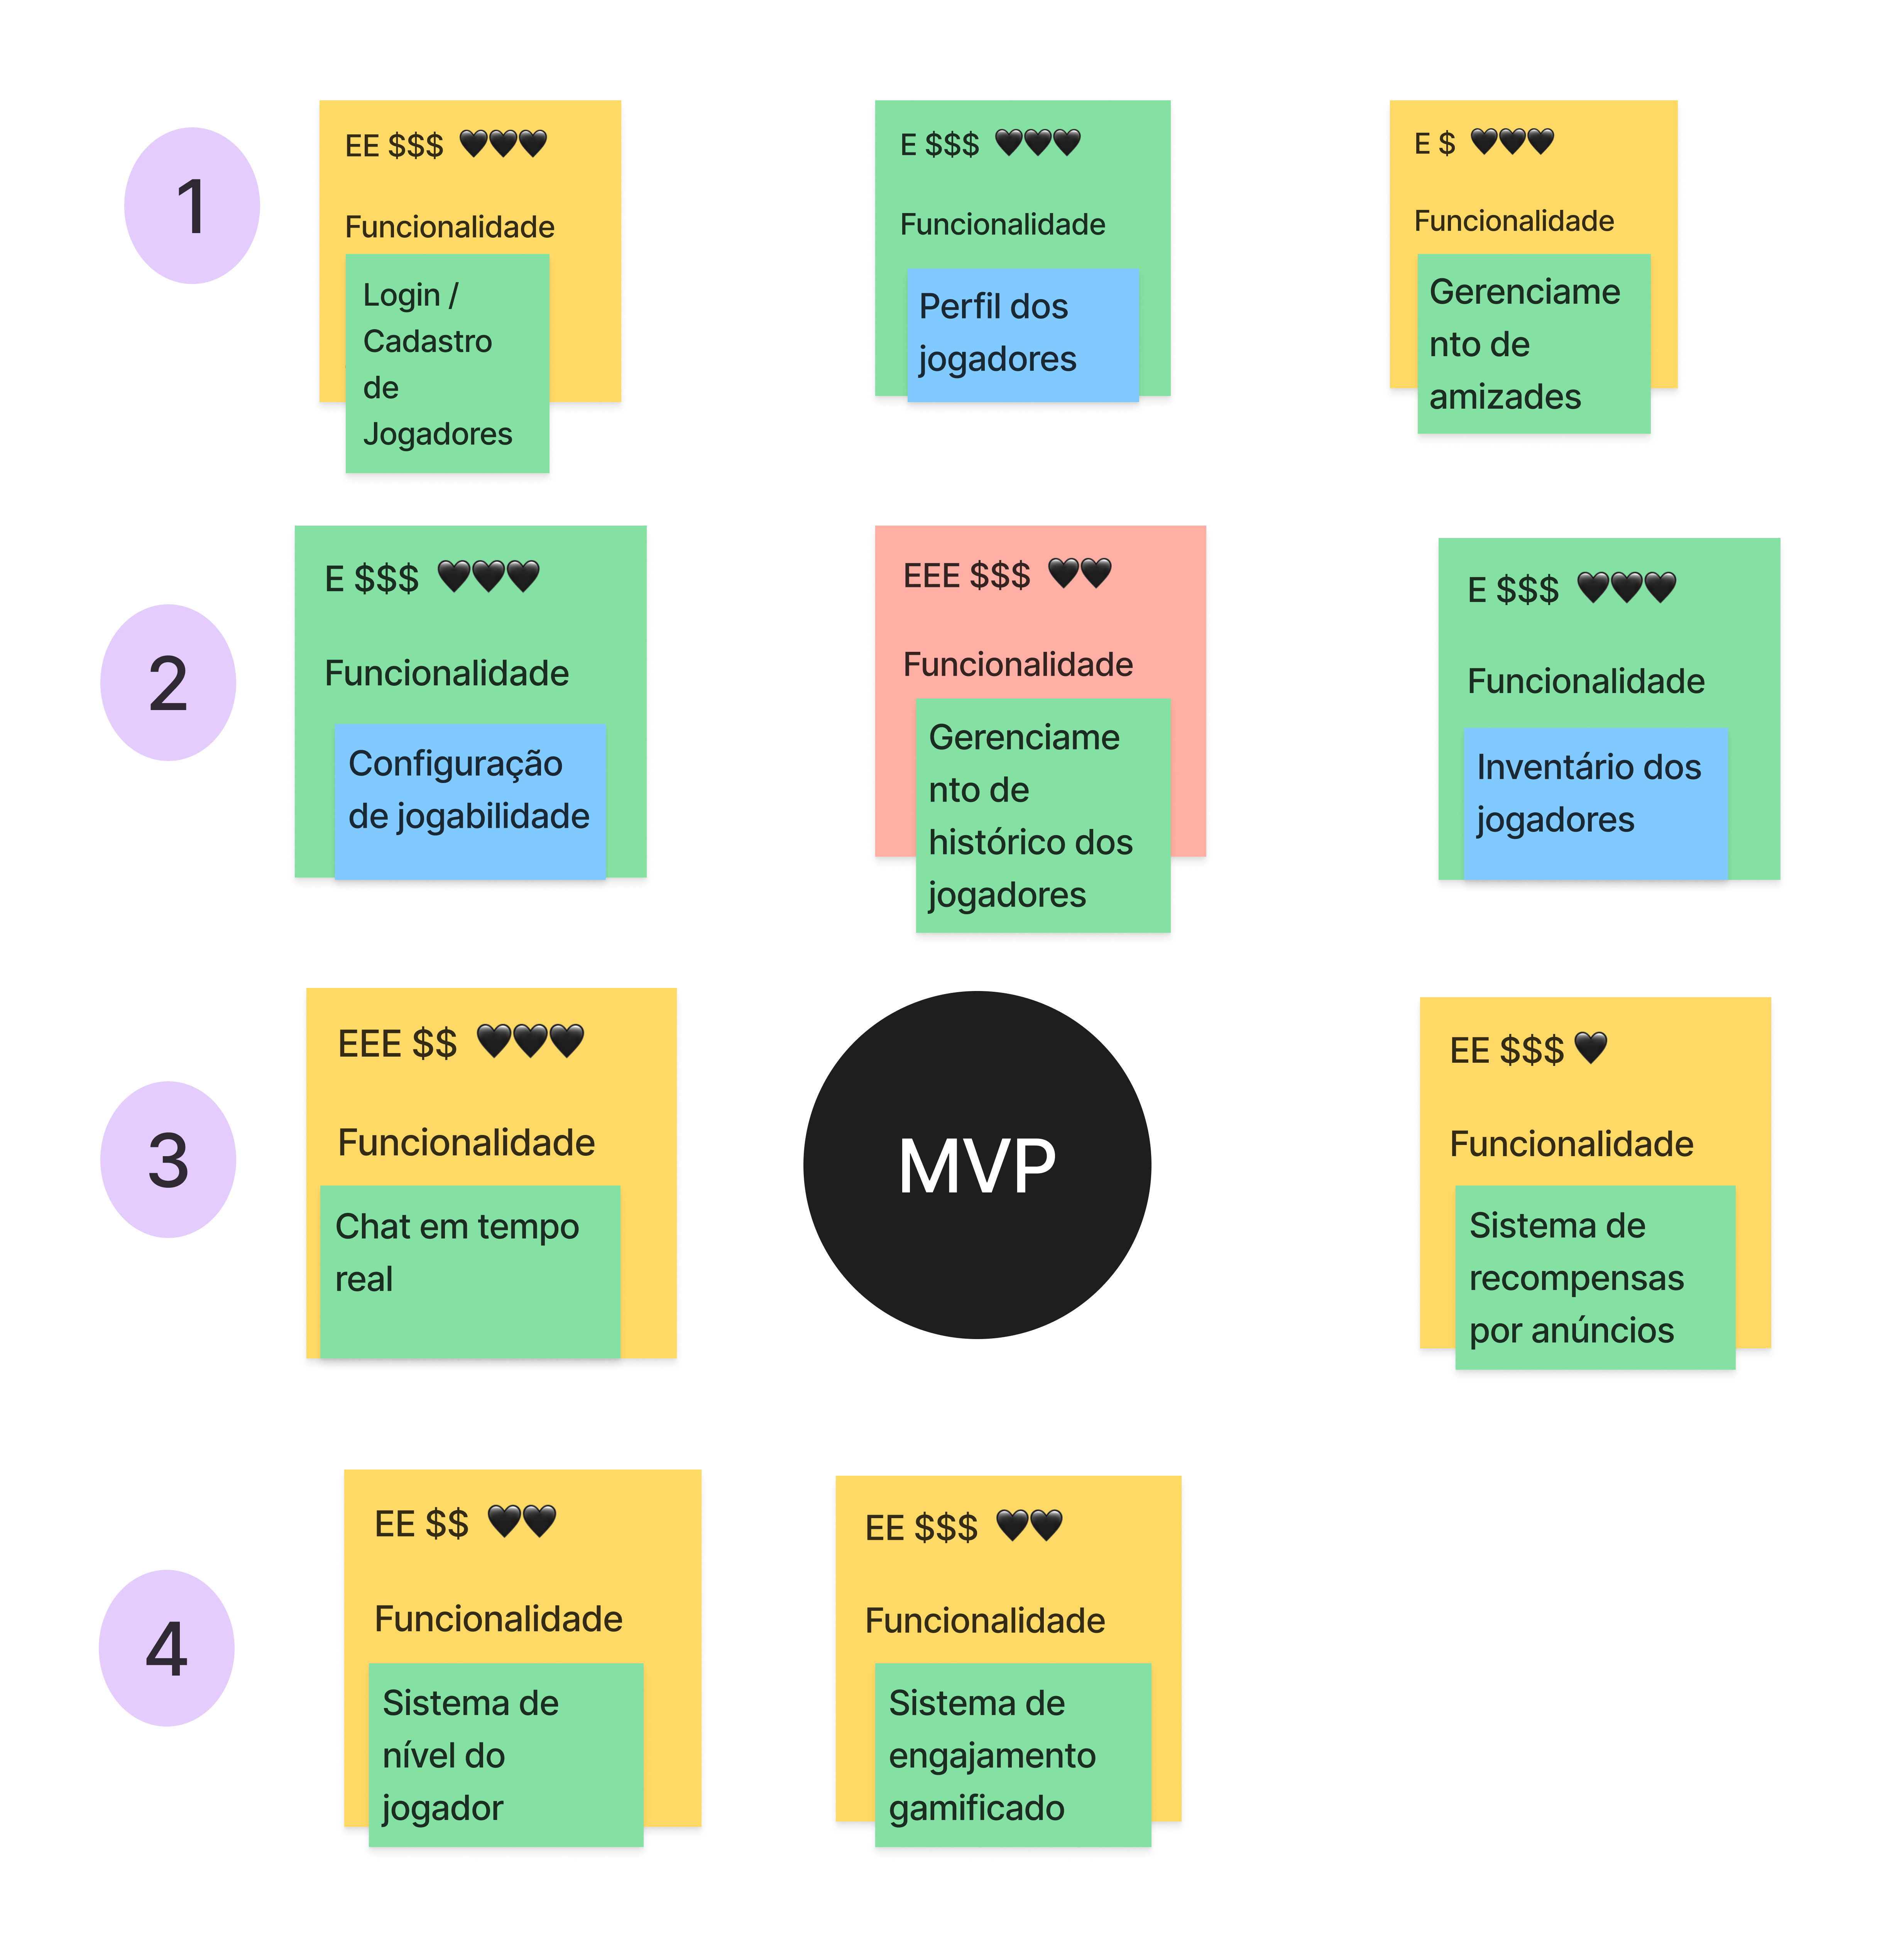
\includegraphics[width=0.9\textwidth]{figuras/Lean14Sequenciador.png}

    Fonte: Adaptado a partir de caroli.org
    
    \vspace{0.2cm}
\end{figure}

\begin{figure}[h!]
    \centering
    \caption{Sequenciador (últimos níveis).} 
    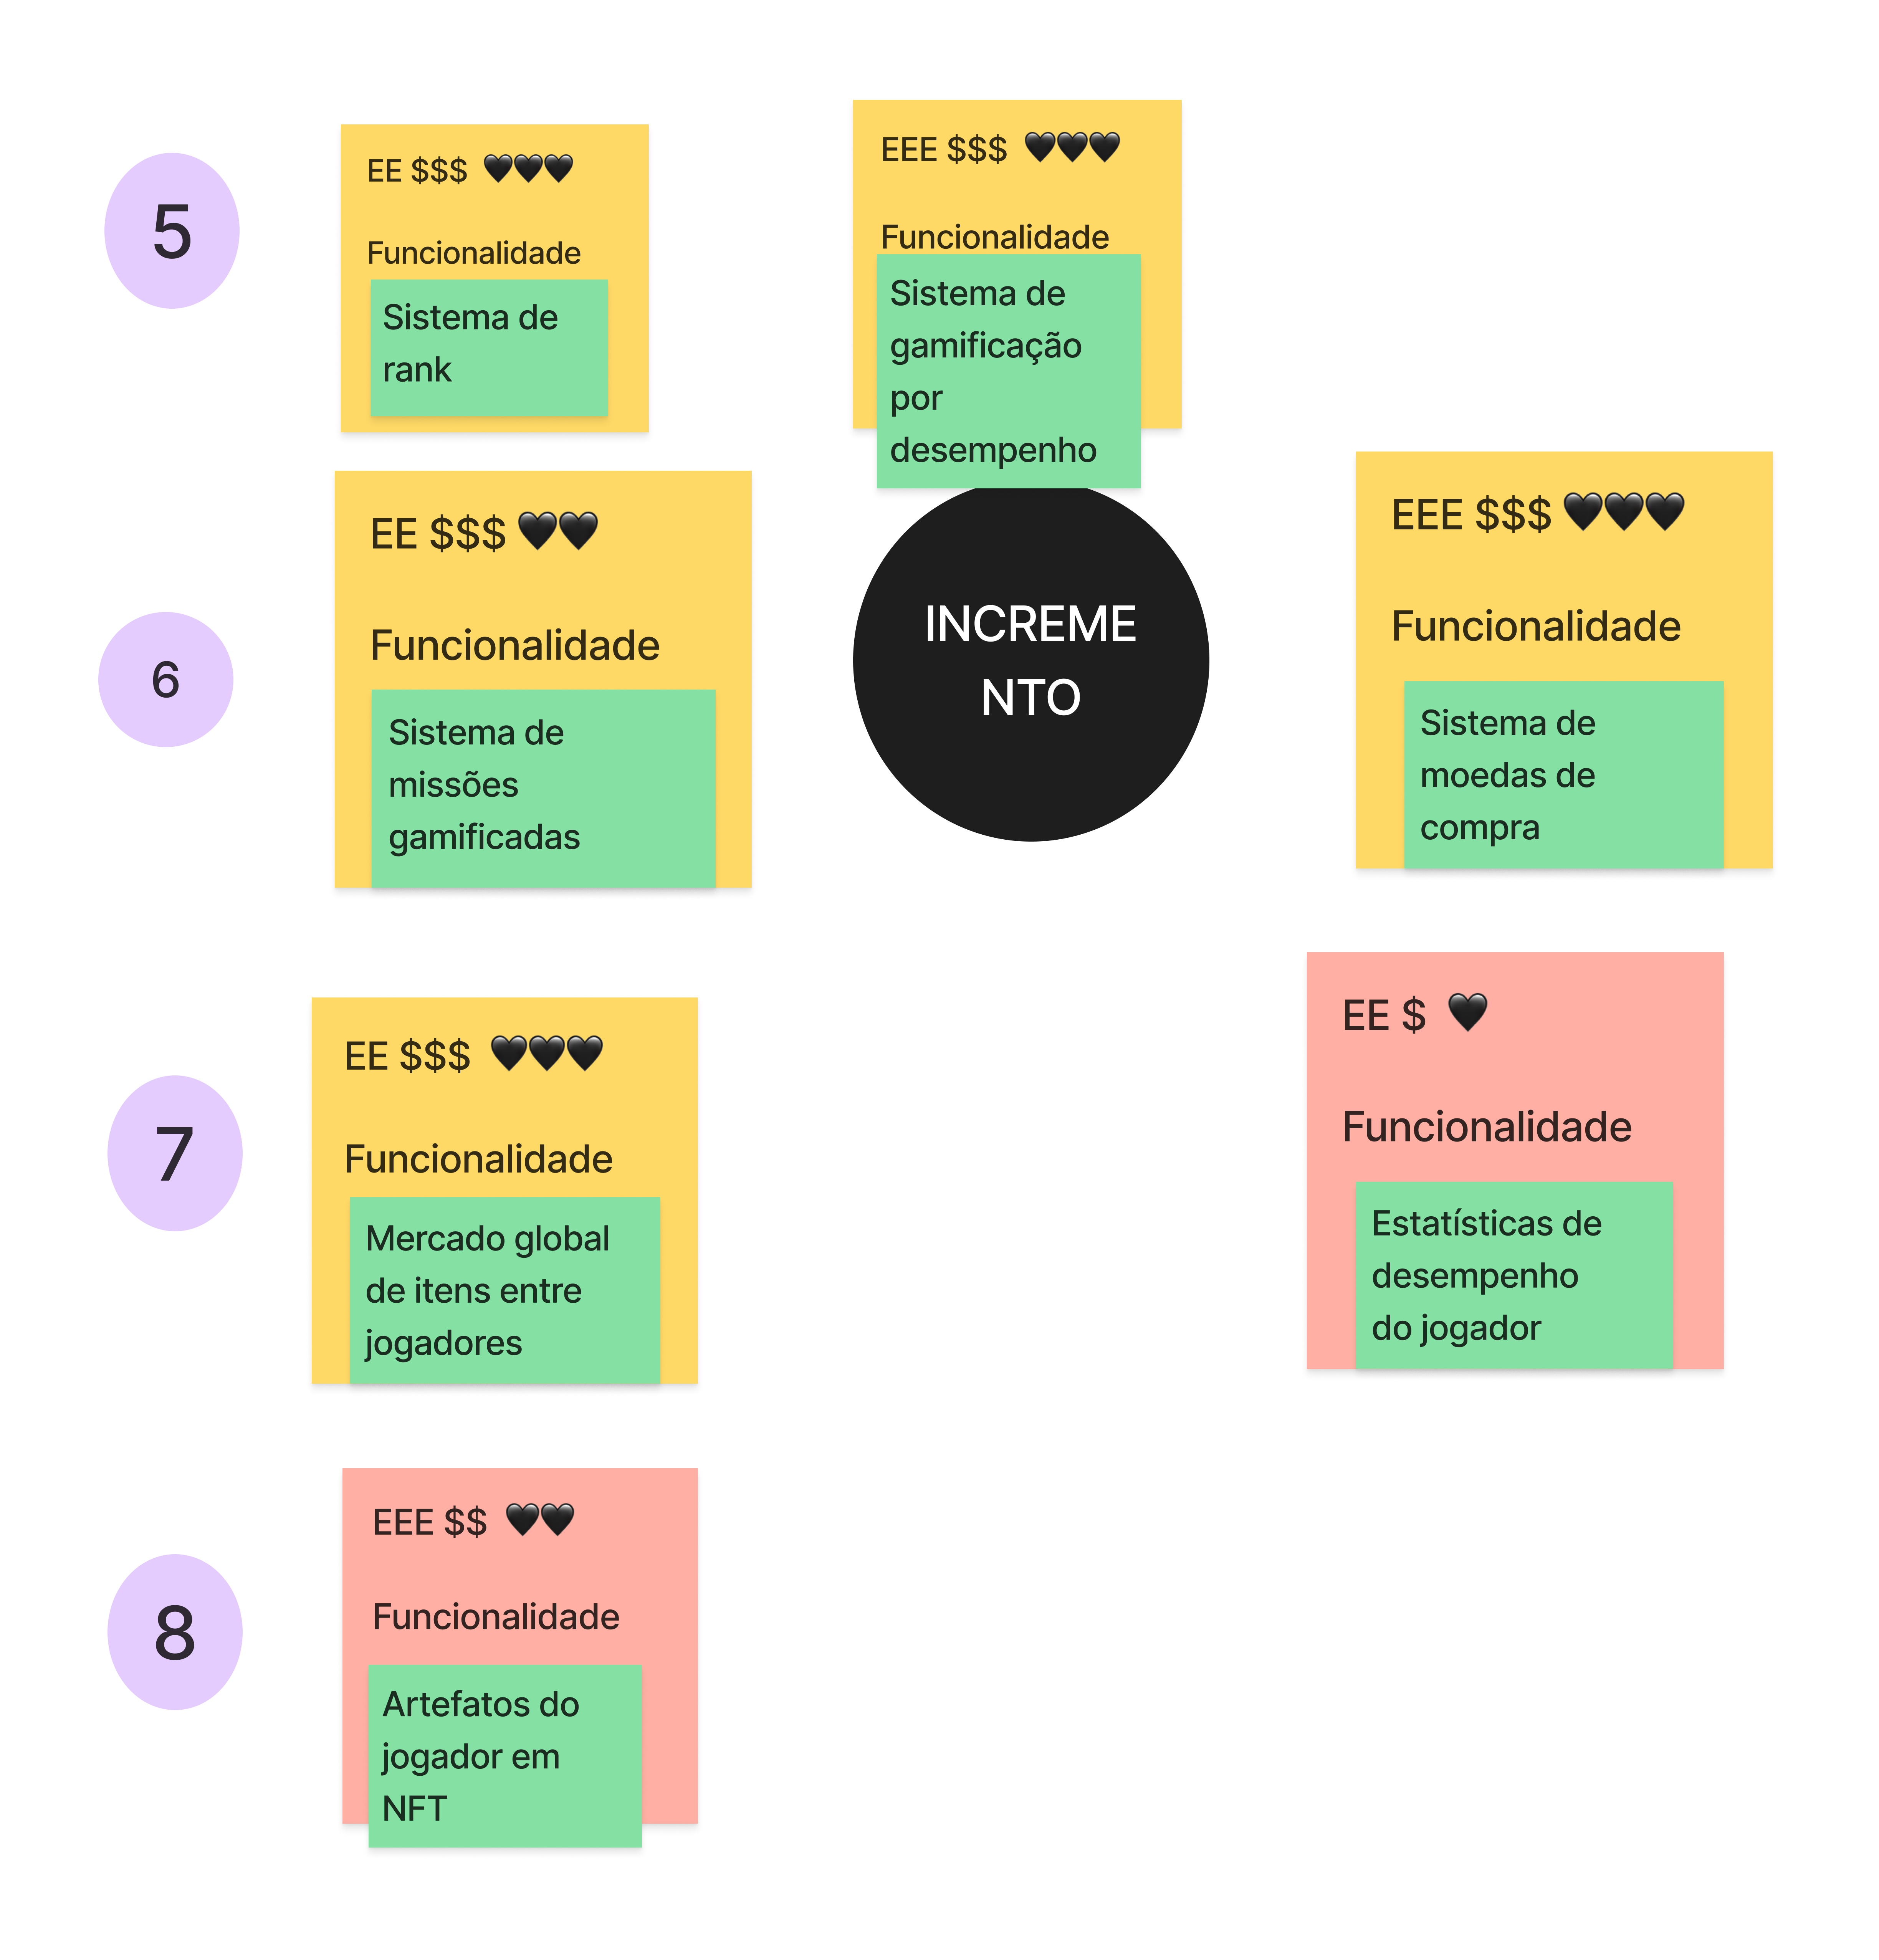
\includegraphics[width=0.9\textwidth]{figuras/Lean14Sequenciador2.png}

    Fonte: Adaptado a partir de caroli.org
    
    \vspace{0.2cm}
\end{figure}

\begin{figure}[h!]
    \centering
    \caption{Canvas MVP.} 
    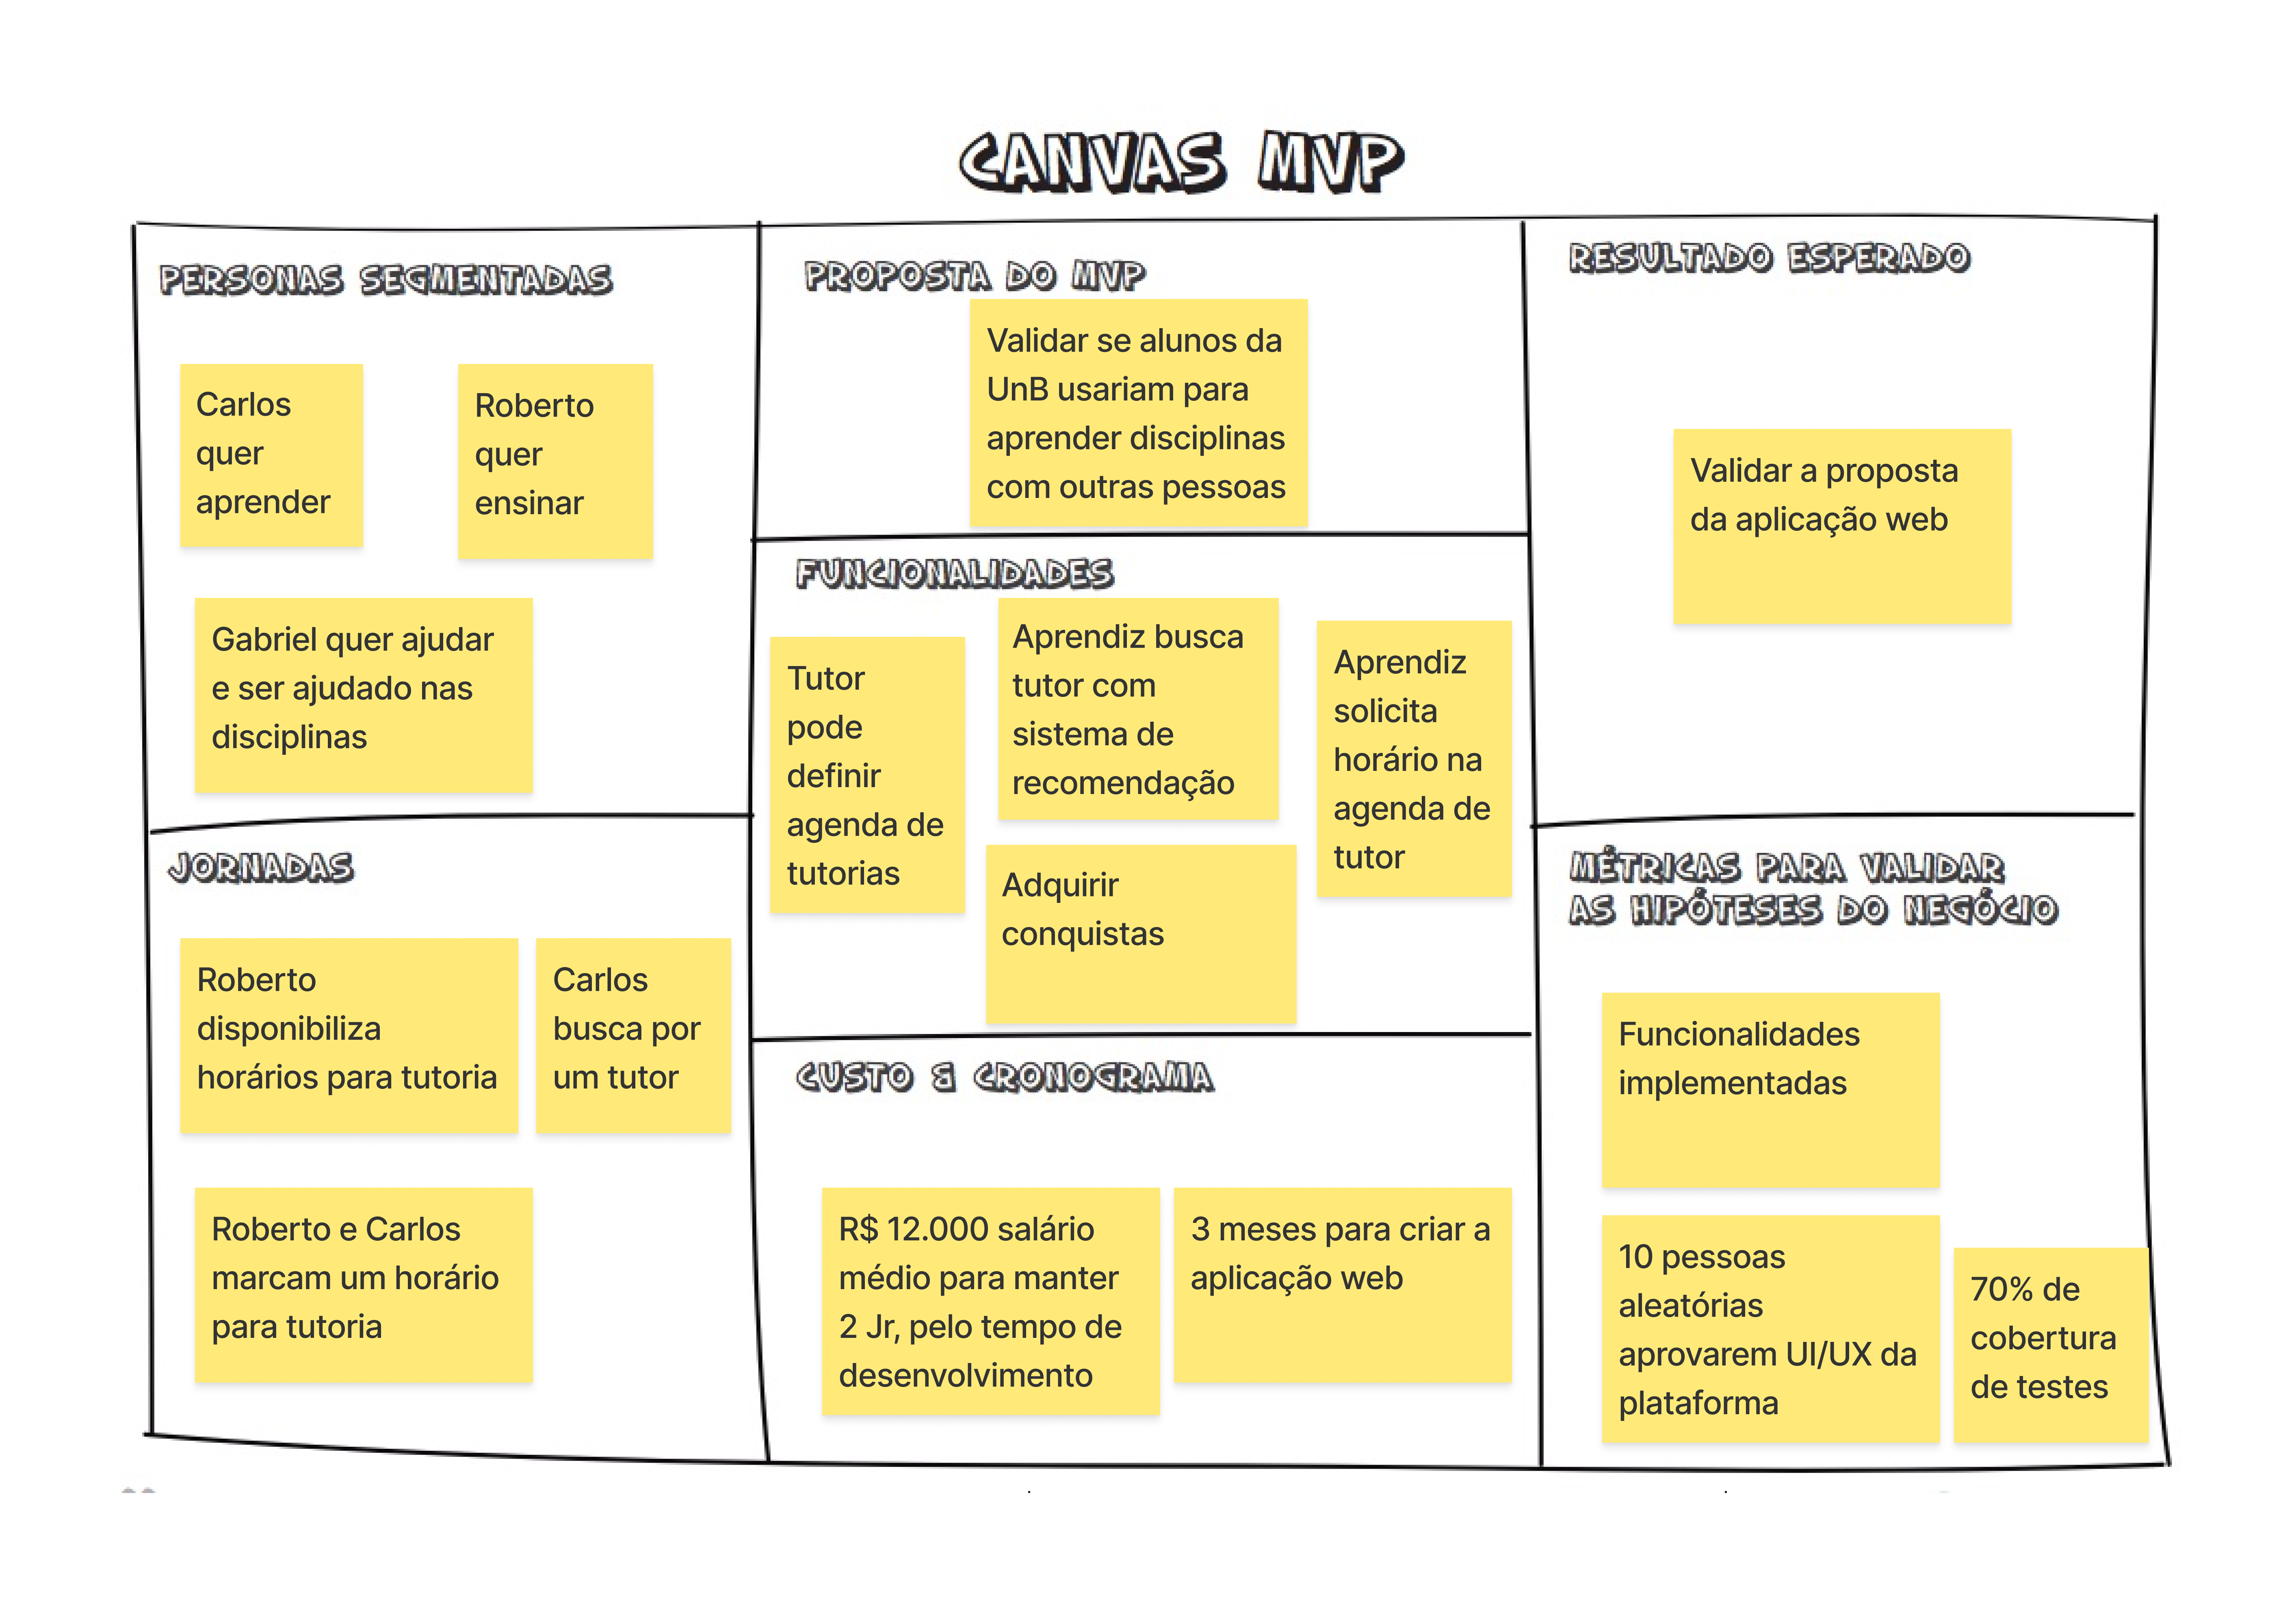
\includegraphics[width=1.1\textwidth]{figuras/Lean15Canvas.png}

    Fonte: Adaptado a partir de caroli.org
    
    \vspace{0.2cm}
\end{figure}

\chapter{Dicionário de Dados}
\label{dicionario-dados}

\section*{USUARIO}
\noindent\textbf{Esclarecimento Técnico:} Tabela proveniente de uma Entidade.\\
\textbf{Descrição:} Define os dados de um Usuário que será cadastrado. 

\begin{table}[h!]
    \centering
    \label{tab:usuario-apendice}
    \resizebox{\linewidth}{!}
    {% Redimensiona a tabela para caber na largura da página
    \begin{tabular}{|l|L{5.5cm}|l|l|L{4cm}|}
        \hline
        \textbf{Atributo} & \textbf{Propriedades do atributo} & \textbf{Tipo de dado} & \textbf{Tamanho} & \textbf{Descrição} \\
        \hline
        usuarioId & chave primária, obrigatório, autoincremento & int & & Número identificador do usuário \\
        \hline
        email & único, obrigatório & varchar & 254 & E-mail do usuário \\
        \hline
        senha & obrigatório & varchar & 256 & Senha criptografada do usuário \\
        \hline
        nomePerfil & obrigatório & varchar & 100 & Nome exibido no perfil do usuário \\
        \hline
        cidade & optativo & varchar & 80 & Cidade onde reside o usuário \\
        \hline
        estado & optativo & char & 2 & Estado onde reside o usuário \\
        \hline
        pontuacao & obrigatório & unsigned int & & Quantidade de pontos obtidos por conquistas do usuário \\
        \hline
        urlFoto & obrigatório & varchar & 256 & URL da foto exibida no perfil do usuário \\
        \hline
        mediaNotaAprendiz & \begin{tabular}[c]{@{}l@{}}derivado de valores na tabela \\ AVALIACAO\_APRENDIZ e \\ não é armazenado por 3ª \\ Forma Normal\end{tabular} & - & - & Média das avaliações do usuário como aprendiz \\
        \hline
    \end{tabular}%
    }
\end{table}

\section*{TUTOR}
\noindent\textbf{Esclarecimento Técnico:} Tabela proveniente de uma Entidade. \\
\textbf{Descrição:} Define os dados de um Tutor que será cadastrado. 

\begin{table}[h!]
\centering
\label{tab:tutor}
\resizebox{\linewidth}{!}{% Redimensiona a tabela para caber na largura da página
    \begin{tabular}{|l|L{3cm}|l|l|l|}
        \hline
        \textbf{Atributo} & \textbf{Propriedades do atributo} & \textbf{Tipo de dado} & \textbf{Tamanho} & \textbf{Descrição} \\
        \hline
        tutorId & chave primária, obrigatório, autoincremento & int & & Número identificador do tutor \\
        \hline
        usuarioId & chave estrangeira, obrigatório & int & & Número identificador do usuário \\
        \hline
    \end{tabular}
}
\end{table}

\section*{AVALIACAO\_APRENDIZ}
\noindent\textbf{Esclarecimento Técnico:} Tabela proveniente de uma Entidade. \\
\textbf{Descrição:} Define os dados de uma avaliação de um aprendiz que será cadastrada.

\begin{table}[h!]
\centering
\label{tab:avaliacao_aprendiz}
    \resizebox{\linewidth}{!}{% Redimensiona a tabela para caber na largura da página
    \begin{tabular}{|l|l|l|l|L{4.5cm}|}
        \hline
        \textbf{Atributo} & \textbf{Propriedades do atributo} & \textbf{Tipo de dado} & \textbf{Tamanho} & \textbf{Descrição} \\
        \hline
        usuarioId & chave estrangeira, obrigatório & int & & Número identificador do usuário \\
        \hline
        nota & obrigatório & int & 1 & Nota fornecida para a avaliação do aprendiz, de 1 a 5. \\
        \hline
        comentario & optativo & varchar & 200 & Comentário fornecido para a avaliação do aprendiz \\
        \hline
    \end{tabular}
    }
\end{table}

\section*{AVALIACAO\_TUTOR}
\noindent\textbf{Esclarecimento Técnico:} Tabela proveniente de uma Entidade. \\
\textbf{Descrição:} Define os dados de uma avaliação de um tutor que será cadastrada.

\begin{table}[h!]
\centering
\label{tab:avaliacao_tutor}
\resizebox{\linewidth}{!}{% Redimensiona a tabela para caber na largura da página
    \begin{tabular}{|l|l|l|l|L{4.5cm}|}
        \hline
        \textbf{Atributo} & \textbf{Propriedades do atributo} & \textbf{Tipo de dado} & \textbf{Tamanho} & \textbf{Descrição} \\
        \hline
        tutorId & chave estrangeira, obrigatório & int & & Número identificador do tutor \\
        \hline
        nota & obrigatório & int & 1 & Nota fornecida para a avaliação do aprendiz, de 1 a 5. \\
        \hline
        comentario & optativo & varchar & 200 & Comentário fornecido para a avaliação do aprendiz \\
        \hline
    \end{tabular}
    }
\end{table}

\section*{AREA}
\noindent\textbf{Esclarecimento Técnico:} Tabela proveniente de uma Entidade.\\
\textbf{Descrição:} Define os dados de uma área de conhecimento que será cadastrada. 
\begin{table}[h!]
\centering
\label{tab:area}
\resizebox{\linewidth}{!}{% Redimensiona a tabela para caber na largura da página
    \begin{tabular}{|l|L{3cm}|l|l|l|}
        \hline
        \textbf{Atributo} & \textbf{Propriedades do atributo} & \textbf{Tipo de dado} & \textbf{Tamanho} & \textbf{Descrição} \\
        \hline
        areaId & chave primária, obrigatório, autoincremento & int & & Número identificador da área \\
        \hline
        nomeArea & único, obrigatório & varchar & 60 & Nome da área de conhecimento \\
        \hline
    \end{tabular}
    }
\end{table}

\section*{ESPECIALIDADE}
\noindent\textbf{Esclarecimento Técnico:} Tabela proveniente de uma Entidade. \\
\textbf{Descrição:} Define os dados de uma especialidade de uma área de conhecimento que será cadastrada. 

\begin{table}[h!]
\centering
\label{tab:especialidade}
\resizebox{\linewidth}{!}{% Redimensiona a tabela para caber na largura da página
\begin{tabular}{|l|L{3.5cm}|l|l|L{4cm}|}
\hline
\textbf{Atributo} & \textbf{Propriedades do atributo} & \textbf{Tipo de dado} & \textbf{Tamanho} & \textbf{Descrição} \\
\hline
especialidadeId & chave primária, obrigatório, autoincremento & int & & Número identificador da especialidade \\
\hline
areaId & chave estrangeira, chave única composta, obrigatório & int & & Número identificador da área de conhecimento \\
\hline
nomeEspecialidade & chave única composta, obrigatório & varchar & 100 & Nome da especialidade \\
\hline
\end{tabular}
}
\end{table}

\section*{CONQUISTA}
\noindent\textbf{Esclarecimento Técnico:} Tabela proveniente de uma Entidade. \\
\textbf{Descrição:} Define os dados de uma conquista que será cadastrada.

\begin{table}[h!]
\centering
\label{tab:conquista}
\resizebox{\linewidth}{!}{% Redimensiona a tabela para caber na largura da página
\begin{tabular}{|l|L{3.5cm}|l|l|L{5cm}|}
\hline
\textbf{Atributo} & \textbf{Propriedades do atributo} & \textbf{Tipo de dado} & \textbf{Tamanho} & \textbf{Descrição} \\
\hline
conquistaId & chave primária, obrigatório, autoincremento & int & & Número identificador da conquista \\
\hline
titulo & único, obrigatório & varchar & 32 & Título da conquista \\
\hline
descricao & obrigatório & varchar & 64 & Descrição do que deve ser feito para conseguir a conquista \\
\hline
urlImagem & obrigatório & varchar & 256 & URL da imagem da conquista \\
\hline
pontos & obrigatório & int & & Quantidade de pontos que serão recompensados ao usuário que conseguir a conquista \\
\hline
\end{tabular}%
}
\end{table}

\section*{CHAT}
\noindent\textbf{Esclarecimento Técnico:} Tabela proveniente de uma Entidade. \\
\textbf{Descrição:} Define os dados de um chat de mensagens entre um tutor e um aprendiz que será cadastrado.

\newpage

\begin{table}[h!]
\centering
\label{tab:chat}
\resizebox{\linewidth}{!}{% Redimensiona a tabela para caber na largura da página
\begin{tabular}{|l|L{3cm}|l|l|l|}
\hline
\textbf{Atributo} & \textbf{Propriedades do atributo} & \textbf{Tipo de dado} & \textbf{Tamanho} & \textbf{Descrição} \\
\hline
chatId & chave primária, obrigatório, autoincremento & int & & Número identificador do chat \\
\hline
tutorId & chave estrangeira, chave única composta, obrigatório & int & & Número identificador do tutor \\
\hline
usuarioId & chave estrangeira, chave única composta, obrigatório & int & & Número identificador do aprendiz \\
\hline
\end{tabular}
}
\end{table}

\section*{MENSAGEM}
\noindent\textbf{Esclarecimento Técnico:} Tabela proveniente de uma Entidade. \\
\textbf{Descrição:} Define os dados de uma mensagem enviada para um chat de mensagens entre um tutor e um aprendiz que será cadastrada.

\begin{table}[h!]
\centering
\label{tab:mensagem}
\resizebox{\linewidth}{!}{% Redimensiona a tabela para caber na largura da página
\begin{tabular}{|l|l|L{3.5cm}|l|L{4cm}|}
\hline
\textbf{Atributo} & \textbf{Propriedades do atributo} & \textbf{Tipo de dado} & \textbf{Tamanho} & \textbf{Descrição} \\
\hline
chatId & chave estrangeira, obrigatório & int & & Número identificador do chat \\
\hline
conteudo & obrigatório & varchar & 200 & Conteúdo textual da mensagem \\
\hline
horario & obrigatório & datetime & & Data e horário de envio da mensagem \\
\hline
remetente & obrigatório & enum('TUTOR', 'APRENDIZ') & & Identificador de quem mandou a mensagem no chat \\
\hline
\end{tabular}
}
\end{table}

\section*{SESSAO}
\noindent\textbf{Esclarecimento Técnico:} Tabela proveniente de uma Entidade. \\
\textbf{Descrição:} Define os dados de uma sessão de tutoria disponível na agenda de um tutor que serão cadastrados.

\newpage

\begin{table}[h!]
\centering
\label{tab:sessao}
\resizebox{\linewidth}{!}{% Redimensiona a tabela para caber na largura da página
\begin{tabular}{|l|L{3cm}|L{3.5cm}|l|L{3.5cm}|}
\hline
\textbf{Atributo} & \textbf{Propriedades do atributo} & \textbf{Tipo de dado} & \textbf{Tamanho} & \textbf{Descrição} \\
\hline
sessaoId & chave primária, obrigatório, autoincremento & int & & Número identificador da sessão \\
\hline
tutorId & chave estrangeira, chave única composta, obrigatório & int & & Número identificador do tutor \\
\hline
dia & chave única composta, obrigatório & enum('SEG', 'TER', 'QUA', 'QUI', 'SEX', 'SAB', 'DOM') & & Dia disponível na agenda do tutor \\
\hline
horarioInicio & chave única composta, obrigatório & time & & Horário de início de uma sessão de tutoria disponível do tutor \\
\hline
horarioFim & obrigatório & time & & Horário de fim de uma sessão de tutoria disponível do tutor \\
\hline
\end{tabular}
}
\end{table}

\section*{SOLICITAÇÃO}
\noindent\textbf{Esclarecimento Técnico:} Tabela proveniente de uma Entidade. \\
\textbf{Descrição:} Define os dados de uma solicitação de sessão de tutoria realizada por um aprendiz que será cadastrada.

\begin{table}[h!]
\centering
\label{tab:solicitacao}
\resizebox{\linewidth}{!}{% Redimensiona a tabela para caber na largura da página
\begin{tabular}{|l|l|L{3cm}|l|L{3cm}|}
\hline
\textbf{Atributo} & \textbf{Propriedades do atributo} & \textbf{Tipo de dado} & \textbf{Tamanho} & \textbf{Descrição} \\
\hline
usuarioId & chave estrangeira, obrigatório & int & & Número identificador do aprendiz \\
\hline
sessaoId & chave estrangeira, obrigatório & int & & Número identificador da sessão \\
\hline
dataCriacao & obrigatório & datetime & & Data e horário da solicitação \\
\hline
validade & obrigatório & datetime & & Data e horário de validade da solicitação \\
\hline
estado & obrigatório & enum('ACEITO', 'PENDENTE', 'RECUSADO', 'RECORRENTE') & & Estado da solicitação \\
\hline
\end{tabular}
}
\end{table}

\section*{CONTEM}
\noindent\textbf{Esclarecimento Técnico:} Tabela proveniente de um Relacionamento.  \\
\textbf{Descrição:} Define relacionamento que corresponde a um relacionamento entre TUTOR e ESPECIALIDADE com cardinalidade \textbf{n:m}.

\begin{table}[h!]
\centering
\label{tab:contem}
\resizebox{\linewidth}{!}{% Redimensiona a tabela para caber na largura da página
\begin{tabular}{|l|L{3.5cm}|l|l|L{3cm}|}
\hline
\textbf{Atributo} & \textbf{Propriedades do atributo} & \textbf{Tipo de dado} & \textbf{Tamanho} & \textbf{Descrição} \\
\hline
especialidadeId & chave estrangeira, chave única composta, obrigatório & int & & Número identificador da especialidade \\
\hline
tutorId & chave estrangeira, chave única composta, obrigatório & int & & Número identificador do tutor \\
\hline
\end{tabular}
}
\end{table}

\section*{CONSEGUE}
\noindent\textbf{Esclarecimento Técnico:} Tabela proveniente de um Relacionamento. \\
\textbf{Descrição:} Define relacionamento que corresponde a um relacionamento entre USUARIO e CONQUISTA com cardinalidade \textbf{n:m}.

\begin{table}[h!]
\centering
\label{tab:consegue}
\resizebox{\linewidth}{!}{% Redimensiona a tabela para caber na largura da página
\begin{tabular}{|l|L{3.5cm}|l|l|l|}
\hline
\textbf{Atributo} & \textbf{Propriedades do atributo} & \textbf{Tipo de dado} & \textbf{Tamanho} & \textbf{Descrição} \\
\hline
usuarioId & chave estrangeira, chave única composta, obrigatório & int & & Número identificador do usuário \\
\hline
conquistaId & chave estrangeira, chave única composta, obrigatório & int & & Número identificador da conquista \\
\hline
\end{tabular}
}
\end{table}

% ----------------
% --- Tabelas geradas pelo Django
% ----------------

\section*{django\_migrations}
\noindent\textbf{Esclarecimento Técnico:} Tabela proveniente de uma Entidade. \\
\textbf{Descrição:} Define quais arquivos \textit{migrations} já foram aplicados na base de dados pelo Django.

\newpage

\begin{table}[h!]
\centering
\label{tab:django_migrations}
\resizebox{\linewidth}{!}{% Redimensiona a tabela para caber na largura da página
\begin{tabular}{|l|L{3.5cm}|l|l|L{3.5cm}|}
\hline
\textbf{Atributo} & \textbf{Propriedades do atributo} & \textbf{Tipo de dado} & \textbf{Tamanho} & \textbf{Descrição} \\
\hline
id & chave primária, obrigatório & bigint & & Número identificador do  django\_migrations\\
\hline
app & obrigatório & varchar & 255 & Define a qual aplicação django se refere \\
\hline
name & obrigatório & varchar & 255 & Define o nome do arquivo \textit{migrations} aplicado \\
\hline
applied & obrigatório & datetime & 6 & Define em que data foi aplicado o \textit{migrations} \\
\hline
\end{tabular}
}
\end{table}

\section*{django\_sessions}
\noindent\textbf{Esclarecimento Técnico:} Tabela proveniente de uma Entidade. \\
\textbf{Descrição:} Define dados relacionado à \textit{login} de sessão do USUARIO.

\begin{table}[h!]
\centering
\label{tab:django_sessions}
\resizebox{\linewidth}{!}{% Redimensiona a tabela para caber na largura da página
\begin{tabular}{|l|L{3.5cm}|l|l|L{3cm}|}
\hline
\textbf{Atributo} & \textbf{Propriedades do atributo} & \textbf{Tipo de dado} & \textbf{Tamanho} & \textbf{Descrição} \\
\hline
id & chave primária, obrigatório & varchar & 40 & Token identificador do  django\_sessions\\
\hline
session\_data & obrigatório & longtext & & Define metadados da sessão\\
\hline
expire\_date & obrigatória & datetime & 6 & Define quando expira a sesão\\
\hline
\end{tabular}
}
\end{table}

\section*{django\_content\_type}
\noindent\textbf{Esclarecimento Técnico:} Tabela proveniente de uma Entidade. \\
\textbf{Descrição:} Define os indíces dos \textit{models}, que foram definidos na aplicação Django.

\newpage

\begin{table}[h!]
\centering
\label{tab:django_content_types}
\resizebox{\linewidth}{!}{% Redimensiona a tabela para caber na largura da página
\begin{tabular}{|l|L{3cm}|l|l|L{4cm}|}
\hline
\textbf{Atributo} & \textbf{Propriedades do atributo} & \textbf{Tipo de dado} & \textbf{Tamanho} & \textbf{Descrição} \\
\hline
id & chave primária, obrigatório & int & & Número identificador do  django\_content\_type\\
\hline
app\_label & obrigatório & varchar & 100 & Define a qual aplicação Django se refere\\
\hline
model & obrigatório & varchar & 100 & Define qual o nome do modelo da aplicação Django se refere\\
\hline
\end{tabular}
}
\end{table}

\section*{django\_admin\_log}
\noindent\textbf{Esclarecimento Técnico:} Tabela proveniente de um Relacionamento. \\
\textbf{Descrição:} Define relacionamento que corresponde a um relacionamento entre USUARIO e django\_content\_type com cardinalidade \textbf{n:m}. É um registro de ações do usuário na página de admin, registra ações do usuário logado com algum \textit{model} da aplicação Django.

\begin{table}[h!]
\centering
\label{tab:django_admin_log}
\resizebox{\linewidth}{!}{% Redimensiona a tabela para caber na largura da página
\begin{tabular}{|l|L{3.5cm}|l|l|L{4cm}|}
\hline
\textbf{Atributo} & \textbf{Propriedades do atributo} & \textbf{Tipo de dado} & \textbf{Tamanho} & \textbf{Descrição} \\
\hline
id & chave primária, obrigatório & int & & Número identificador do  django\_admin\_log\\
\hline
usuarioId & chave estrangeira, obrigatória & int & & Número identificador do USUARIO\\
\hline
djngo\_content\_type & chave estrangeira, obrigatória & int & & Número identificador do django\_content\_type\\
\hline
action\_time & obrigatório & datetime & 6 & Define em que data ocorreu o registro\\
\hline
object\_id & obrigatório & longtext & & Define o id do objeto que foi alvo da ação do usuário\\
\hline
object\_repr & opcional & varchar & 200 & Define o nome do objeto que está sendo alterado\\
\hline
action\_flag & obriatório & smallint & & Define qual ação o usuário executou, sendo 1 criação, 2 modificação e 3 deleção do objeto\\
\hline
change\_message & opcional & longtext & & Define uma mensagem para este registro\\
\hline
\end{tabular}
}
\end{table}


\section*{auth\_permission}
\noindent\textbf{Esclarecimento Técnico:} Tabela proveniente de uma Entidade. \\
\textbf{Descrição:} Define permissão para um USUARIO autenticado em relação à um \textit{model}.

\begin{table}[h!]
\centering
\label{tab:auth_permission}
\resizebox{\linewidth}{!}{% Redimensiona a tabela para caber na largura da página
\begin{tabular}{|l|L{3.5cm}|l|l|L{4cm}|}
\hline
\textbf{Atributo} & \textbf{Propriedades do atributo} & \textbf{Tipo de dado} & \textbf{Tamanho} & \textbf{Descrição} \\
\hline
id & chave primária, obrigatório & int & & Número identificador do  auth\_permission\\
\hline
django\_content\_type & chave estrangeira, obrigatória & int & & Número identificador do django\_content\_type\\
\hline
name & obrigatório & varchar & 255 & Define uma descrição para esta permissão, Ex: Adicionar conquista ao usuário\\
\hline
codename & obrigatório & datetime & 6 & Define um nome curto para esta permissão, Ex: add\_conquista\\
\hline
\end{tabular}
}
\end{table}

\section*{auth\_group}
\noindent\textbf{Esclarecimento Técnico:} Tabela proveniente de uma Entidade. \\
\textbf{Descrição:} Define grupos para USUARIO. Estes grupos podem separar USUARIO por cargo, função ou papel.

\begin{table}[h!]
\centering
\label{tab:auth_group}
\resizebox{\linewidth}{!}{% Redimensiona a tabela para caber na largura da página
\begin{tabular}{|l|L{3.5cm}|l|l|l|}
\hline
\textbf{Atributo} & \textbf{Propriedades do atributo} & \textbf{Tipo de dado} & \textbf{Tamanho} & \textbf{Descrição} \\
\hline
id & chave primária, obrigatório & int & & Número identificador do  auth\_group\\
\hline
name & obrigatório & varchar & 150 & Define o nome do grupo\\
\hline
\end{tabular}
}
\end{table}

\section*{auth\_group\_permissions}
\noindent\textbf{Esclarecimento Técnico:} Tabela proveniente de um Relacionamento. \\
\textbf{Descrição:} Define relacionamento que corresponde a um relacionamento entre auth\_group e auth\_permission com cardinalidade \textbf{n:m}.

\begin{table}[h!]
\centering
\label{tab:auth_group_permissions}
\resizebox{\linewidth}{!}{% Redimensiona a tabela para caber na largura da página
\begin{tabular}{|l|L{3.5cm}|l|l|L{4.5cm}|}
\hline
\textbf{Atributo} & \textbf{Propriedades do atributo} & \textbf{Tipo de dado} & \textbf{Tamanho} & \textbf{Descrição} \\
\hline
id & chave primária, obrigatório & int & & Número identificador do  auth\_group\_permissions\\
\hline
auth\_permission\_id & chave estrangeira, obrigatório & int & & Número identificador do  auth\_permissions\\
\hline
auth\_group\_id & chave estrangeira, obrigatório & int & & Número identificador do  auth\_group\\
\hline
\end{tabular}
}
\end{table}

\section*{USUARIO\_groups}
\noindent\textbf{Esclarecimento Técnico:} Tabela proveniente de um Relacionamento. \\
\textbf{Descrição:} Define relacionamento que corresponde a um relacionamento entre USUARIO e auth\_group com cardinalidade \textbf{n:m}.

\begin{table}[h!]
\centering
\label{tab:USUARIO_groups}
\resizebox{\linewidth}{!}{% Redimensiona a tabela para caber na largura da página
\begin{tabular}{|l|L{3.5cm}|l|l|L{4cm}|}
\hline
\textbf{Atributo} & \textbf{Propriedades do atributo} & \textbf{Tipo de dado} & \textbf{Tamanho} & \textbf{Descrição} \\
\hline
id & chave primária, obrigatório & bigint & & Número identificador do  USUARIO\_groups\\
\hline
usuarioId & chave estrangeira, obrigatória & int & & Número identificador do USUARIO\\
\hline
auth\_group\_id & chave estrangeira, obrigatória & int & & Número identificador do auth\_group\\
\hline
\end{tabular}
}
\end{table}

\section*{USUARIO\_permissions}
\noindent\textbf{Esclarecimento Técnico:} Tabela proveniente de um Relacionamento. \\
\textbf{Descrição:} Define relacionamento que corresponde a um relacionamento entre USUARIO e auth\_group com cardinalidade \textbf{n:m}.

\begin{table}[H]
\centering
\label{tab:USUARIO_permissions}
\resizebox{\linewidth}{!}{% Redimensiona a tabela para caber na largura da página
\begin{tabular}{|l|L{3.5cm}|l|l|L{4cm}|}
\hline
\textbf{Atributo} & \textbf{Propriedades do atributo} & \textbf{Tipo de dado} & \textbf{Tamanho} & \textbf{Descrição} \\
\hline
id & chave primária, obrigatório & bigint & & Número identificador do  USUARIO\_groups\\
\hline
usuarioId & chave estrangeira, obrigatória & int & & Número identificador do USUARIO\\
\hline
auth\_group\_id & chave estrangeira, obrigatória & int & & Número identificador do auth\_group\\
\hline
\end{tabular}
}
\end{table}


% \chapter{Primeiro Anexo}

% Texto do primeiro anexo.

% \chapter{Segundo Anexo}

% Texto do segundo anexo.

% \partapendices
% \chapter{Primeiro Apêndice}

% Texto do primeiro apêndice.

% \chapter{Segundo Apêndice}

% Texto do segundo apêndice.

\end{apendicesenv}



% \input{editaveis/anexos}
\printindex

\end{document}

